\documentclass[a4paper]{article}
\usepackage[margin=1.0in]{geometry}
\usepackage{longtable}
\usepackage{graphicx}
\usepackage{grffile}

\title{Metabolomic Data Analysis with MetaboAnalyst 5.0}
\author{ Name: guest18358687840321369509 }
\usepackage{Sweave}
\begin{document}
\parskip=.3cm
\maketitle
\section{Background}
 The Pathway Analysis module combines results from powerful pathway  enrichment analysis with pathway topology analysis to help researchers identify the most relevant pathways involved in the conditions under study. 

 There are many commercial pathway analysis software tools such as Pathway Studio, MetaCore, or Ingenuity Pathway Analysis (IPA), etc. Compared to these commercial tools, the pathway analysis module was specifically developed  for metabolomics studies. It uses high-quality KEGG metabolic pathways as the backend knowledgebase.  This module integrates many well-established (i.e. univariate analysis, over-representation analysis) methods, as well as novel algorithms and concepts (i.e. Global Test, GlobalAncova, network topology analysis) into pathway analysis. Another feature is a Google-Map style interactive visualization system to deliver  the analysis results in an intuitive manner.
\section{Data Input}
 The Pathway Analysis module accepts either a list of compound labels (common names, HMDB IDs or KEGG IDs) with one compound per row,  or a compound concentration table with samples in rows and compounds in columns. The second column must be  phenotype labels (binary, multi-group, or continuous). The table is uploaded as comma separated values (.csv). 

\section{Compound Name Matching}

The first step is to standardize the compound labels used in user uploaded data. This is a necessary step since
these compounds will be subsequently compared with compounds contained in the pathway library.
There are three outcomes from the step - exact match, approximate match (for common names only), and no match.
Users should click the textbf{View} button from the approximate matched results to manually select the correct one.
Compounds without match will be excluded from the subsequently pathway analysis.



\textbf{Table 1} shows the conversion results. Note: \textit{1} indicates exact match, \textit{2}
indicates approximate match, and \textit{0} indicates no match. A text file contain the result can be
found the downloaded file \textit{name\_map.csv}


% latex table generated in R 4.1.3 by xtable 1.8-4 package
% Sat Feb 18 08:43:43 2023
\begingroup\scriptsize
\begin{longtable}{rlllllll}
\caption{Result from Compound Name Mapping} \\ 
  \hline
 & Query & Match & HMDB & PubChem & KEGG & SMILES & Comment \\ 
  \hline
1 & (-)-Camphanic acid & NA & NA & NA & NA & NA & 0 \\ 
  2 & (+)-Epicatechin & (+)-Epicatechin & HMDB0037954 & 182232 & C09728 & O[C@H]1CC2=C(O)C=C(O)C=C2O[C@H]1C1=CC(O)=C(O)C=C1 & 1 \\ 
  3 & (10E,15Z)-9,12,13-trihydroxyoctadeca-10,15-dienoic acid & NA & NA & NA & NA & NA & 0 \\ 
  4 & (1R,3R,4S,5R)-1,3,4-trihydroxy-5-[(E)-3-(4-hydroxy-3-methoxyphenyl)prop-2-enoyl]oxycyclohexane-1-carboxylic acid & NA & NA & NA & NA & NA & 0 \\ 
  5 & (1R,3R,4S,5R)-1,3,4-trihydroxy-5-[(E)-3-(4-hydroxyphenyl)prop-2-enoyl]oxycyclohexane-1-carboxylic acid & NA & NA & NA & NA & NA & 0 \\ 
  6 & (1r,3R,4s,5S)-4-\{[(2E)-3-(3,4-Dihydroxyphenyl)-2-propenoyl]oxy\}-1,3,5-trihydroxycyclohexanecarboxylic acid & NA & NA & NA & NA & NA & 0 \\ 
  7 & (1S,3R,4S,5R)-4-\{[(2E)-3-(3,4-dihydroxyphenyl)prop-2-enoyl]oxy\}-1,3,5-trihydroxycyclohexane-1-carboxylic acid & NA & NA & NA & NA & NA & 0 \\ 
  8 & (2R,3R,4S,5S,6R)-2-[[7-hydroxy-1-(4-hydroxy-3-methoxyphenyl)-3-(hydroxymethyl)-6-methoxy-1,2,3,4-tetrahydronaphthalen-2-yl]methoxy]-6-(hydroxymethyl)oxane-3,4,5-triol & NA & NA & NA & NA & NA & 0 \\ 
  9 & (2R,3S,4S,5R,6R)-2-(hydroxymethyl)-6-[4-(4-hydroxy-2,6,6-trimethylcyclohexen-1-yl)butan-2-yloxy]oxane-3,4,5-triol & NA & NA & NA & NA & NA & 0 \\ 
  10 & (2R,3S,4S,5R,6R)-2-[[(2R,3R,4R,5S)-3,4-dihydroxy-5-(hydroxymethyl)oxolan-2-yl]oxymethyl]-6-[(2E)-3,7-dimethylocta-2,6-dienoxy]oxane-3,4,5-triol & NA & NA & NA & NA & NA & 0 \\ 
  11 & (2R,3S,4S,5R,6S)-2-(hydroxymethyl)-6-[4-(hydroxymethyl)-1-propan-2-ylcyclohex-3-en-1-yl]oxyoxane-3,4,5-triol & NA & NA & NA & NA & NA & 0 \\ 
  12 & (2S,3R,4S,5R)-2-[(2R,3R,4S,5S,6R)-4,5-dihydroxy-6-(hydroxymethyl)-2-(2-phenylethoxy)oxan-3-yl]oxyoxane-3,4,5-triol & NA & NA & NA & NA & NA & 0 \\ 
  13 & (2S,3R,4S,5S,6R)-2-[3-hydroxy-5-[(Z)-2-(4-hydroxyphenyl)ethenyl]phenoxy]-6-(hydroxymethyl)oxane-3,4,5-triol & NA & NA & NA & NA & NA & 0 \\ 
  14 & (2S,3S,4S,5R,6R)-6-(3-benzoyloxy-2-hydroxypropoxy)-3,4,5-trihydroxyoxane-2-carboxylic acid & NA & NA & NA & NA & NA & 0 \\ 
  15 & (3aS,5R,5aS,8aS,9aR)-5,8a-dimethyl-1-methylidene-3a,4,5,5a,6,7,9,9a-octahydroazuleno[6,7-b]furan-2,8-dione & NA & NA & NA & NA & NA & 0 \\ 
  16 & (4S,5Z,6S)-4-(2-methoxy-2-oxoethyl)-5-[2-[(E)-3-phenylprop-2-enoyl]oxyethylidene]-6-[(2S,3R,4S,5S,6R)-3,4,5-trihydroxy-6-(hydroxymethyl)oxan-2-yl]oxy-4H-pyran-3-carboxylic acid & NA & NA & NA & NA & NA & 0 \\ 
  17 & (9Z,12E)-15,16-dihydroxyoctadeca-9,12-dienoic acid & NA & NA & NA & NA & NA & 0 \\ 
  18 & (E)-3-[4-[(2S,3R,4S,5S,6R)-3,4,5-trihydroxy-6-(hydroxymethyl)oxan-2-yl]oxyphenyl]prop-2-enoic acid & NA & NA & NA & NA & NA & 0 \\ 
  19 & (Z)-5,8,11-trihydroxyoctadec-9-enoic acid & NA & NA & NA & NA & NA & 0 \\ 
  20 & [(2R,3S,4S,5R,6R)-6-[(2S,3S,4S,5R)-3,4-dihydroxy-2,5-bis(hydroxymethyl)oxolan-2-yl]oxy-3,4,5-trihydroxyoxan-2-yl]methyl 4-hydroxybenzoate & NA & NA & NA & NA & NA & 0 \\ 
  21 & [(2S,3R,4S,5S,6R)-3,4,5-trihydroxy-6-(hydroxymethyl)oxan-2-yl] (2E,6E)-8-hydroxy-2,6-dimethylocta-2,6-dienoate & NA & NA & NA & NA & NA & 0 \\ 
  22 & [(4E)-7-acetyloxy-6-hydroxy-2-methyl-10-oxo-2,3,6,7,8,9-hexahydrooxecin-3-yl] (E)-but-2-enoate & NA & NA & NA & NA & NA & 0 \\ 
  23 & [3,4,5-trihydroxy-6-(3,4,5-trihydroxybenzoyl)oxyoxan-2-yl]methyl 3,4,5-trihydroxybenzoate & NA & NA & NA & NA & NA & 0 \\ 
  24 & [3,4,5-trihydroxy-6-[[3,4,5-trihydroxy-6-(hydroxymethyl)oxan-2-yl]oxymethyl]oxan-2-yl] 2,6,6-trimethylcyclohexene-1-carboxylate & NA & NA & NA & NA & NA & 0 \\ 
  25 & 1-(4-hydroxyphenyl)-3-[(2R,3R,4S,5S,6R)-3,4,5-trihydroxy-6-(hydroxymethyl)oxan-2-yl]oxypropan-1-one & NA & NA & NA & NA & NA & 0 \\ 
  26 & 1-[3-methoxy-4-[(2S,3R,4S,5S,6R)-3,4,5-trihydroxy-6-[[(2R,3R,4R,5R,6S)-3,4,5-trihydroxy-6-methyloxan-2-yl]oxymethyl]oxan-2-yl]oxyphenyl]ethanone & NA & NA & NA & NA & NA & 0 \\ 
  27 & 1,2-dihydroxyheptadec-16-en-4-yl acetate & NA & NA & NA & NA & NA & 0 \\ 
  28 & 1H-2-benzopyran-1-one, 6,8-dihydroxy-3-methyl- & NA & NA & NA & NA & NA & 0 \\ 
  29 & 2-(3-hydroxy-5-methoxyphenoxy)-6-(hydroxymethyl)oxane-3,4,5-triol & NA & NA & NA & NA & NA & 0 \\ 
  30 & 2-(3,4-dihydroxyphenyl)-5,7-dihydroxy-6,8-dimethoxychromen-4-one & NA & NA & NA & NA & NA & 0 \\ 
  31 & 2-[1-hydroxy-1-(4-methoxyphenyl)propan-2-yl]oxy-6-(hydroxymethyl)oxane-3,4,5-triol & NA & NA & NA & NA & NA & 0 \\ 
  32 & 2-[2-[(Z)-pent-2-enyl]-3-[3,4,5-trihydroxy-6-(hydroxymethyl)oxan-2-yl]oxycyclopentyl]acetic acid & NA & NA & NA & NA & NA & 0 \\ 
  33 & 2-[4-[4-[hydroxy-(4-hydroxy-3-methoxyphenyl)methyl]-3-(hydroxymethyl)oxolan-2-yl]-2-methoxyphenoxy]-6-(hydroxymethyl)oxane-3,4,5-triol & NA & NA & NA & NA & NA & 0 \\ 
  34 & 3-[4-methoxy-2-[(2S,3R,4S,5S,6R)-3,4,5-trihydroxy-6-(hydroxymethyl)oxan-2-yl]oxyphenyl]propanoic acid & NA & NA & NA & NA & NA & 0 \\ 
  35 & 3-[5,7-dihydroxy-2-(4-methoxyphenyl)-4-oxo-2,3-dihydrochromen-3-yl]-5,7-dihydroxy-2-(4-methoxyphenyl)-2,3-dihydrochromen-4-one & NA & NA & NA & NA & NA & 0 \\ 
  36 & 3-Hydroxycinnamic acid & m-Coumaric acid & HMDB0001713 & 637541 & C12621 & C1=CC(=CC(=C1)O)/C=C/C(=O)O & 1 \\ 
  37 & 3-methylquercetin & Isorhamnetin & HMDB0002655 & 5281654 & C10084 & COC1=C(C=CC(=C1)C2=C(C(=O)C3=C(C=C(C=C3O2)O)O)O)O & 1 \\ 
  38 & 3-O-Feruloylquinic acid & 3-O-Feruloylquinic acid & HMDB0030669 & 131751068 & C02572 & COC1=C(O)C=C($\backslash$C=C/C(=O)OC2CC(O)(CC(O)C2O)C(O)=O)C=C1 & 1 \\ 
  39 & 4-[2-(6,7-dihydroxy-1,2,4a-trimethylspiro[3,4,6,7,8,8a-hexahydro-2H-naphthalene-5,2-oxirane]-1-yl)ethyl]-2-hydroxy-2H-furan-5-one & NA & NA & NA & NA & NA & 0 \\ 
  40 & 4-O-Methylphloracetophenone & Phloretin & HMDB0003306 & 4788 & C00774 & C1=CC(=CC=C1CCC(=O)C2=C(C=C(C=C2O)O)O)O & 1 \\ 
  41 & 4,5,7-trihydroxy-3,6-dimethoxyflavone & NA & NA & NA & NA & NA & 0 \\ 
  42 & 6-Methoxy-7-hydroxycoumarin & Scopoletin & HMDB0034344 & 5280460 & C01752 & COC1=C(C=C2C(=C1)C=CC(=O)O2)O & 1 \\ 
  43 & 7-ethenyl-1,4a,7-trimethyl-6-oxo-2,3,4,8,8a,9,10,10a-octahydrophenanthrene-1-carboxylic acid & NA & NA & NA & NA & NA & 0 \\ 
  44 & 7-hydroxy-2-(4-hydroxy-3,5-dimethoxyphenyl)-5-[(2S,3R,4S,5S,6R)-3,4,5-trihydroxy-6-(hydroxymethyl)oxan-2-yl]oxychromen-4-one & NA & NA & NA & NA & NA & 0 \\ 
  45 & 7,8-Dihydroxycoumarin & NA & NA & NA & NA & NA & 0 \\ 
  46 & 8-[3-oxo-2-[(E)-pent-2-enyl]cyclopenten-1-yl]octanoic acid & NA & NA & NA & NA & NA & 0 \\ 
  47 & 9-hydroxy-10,12-octadecadienoic acid & Alpha-dimorphecolic acid & HMDB0004670 & 5312830 & C14767 & CCCCC/C=C$\backslash$C=C$\backslash$[C@H](CCCCCCCC(=O)O)O & 1 \\ 
  48 & afzelechin & Afzelechin & HMDB0030823 & 282014 & C09320 & C1C(C(OC2=CC(=CC(=C21)O)O)C3=CC=C(C=C3)O)O & 1 \\ 
  49 & Anhydrobrazilic Acid & NA & NA & NA & NA & NA & 0 \\ 
  50 & astilbin & Astilbin & HMDB0033850 & 119258 & C17449 & C[C@H]1[C@@H]([C@H]([C@H]([C@@H](O1)O[C@@H]2[C@H](OC3=CC(=CC(=C3C2=O)O)O)C4=CC(=C(C=C4)O)O)O)O)O & 1 \\ 
  51 & Biochanin A & Biochanin A & HMDB0002338 & 5280373 & C00814 & COC1=CC=C(C=C1)C2=COC3=CC(=CC(=C3C2=O)O)O & 1 \\ 
  52 & Brazilein & NA & NA & NA & NA & NA & 0 \\ 
  53 & Cholic Acid & Cholic acid & HMDB0000619 & 221493 & C00695 & C[C@H](CCC(=O)O)[C@H]1CC[C@@H]2[C@@]1([C@H](C[C@H]3[C@H]2[C@@H](C[C@H]4[C@@]3(CC[C@H](C4)O)C)O)O)C & 1 \\ 
  54 & Chrysin & Chrysin & HMDB0036619 & 5281607 & C10028 & OC1=CC(O)=C2C(=O)C=C(OC2=C1)C1=CC=CC=C1 & 1 \\ 
  55 & D-(-)-quinic acid & NA & NA & NA & NA & NA & 0 \\ 
  56 & Daidzein-8-C-glucoside & NA & NA & NA & NA & NA & 0 \\ 
  57 & Deoxycholic Acid & Deoxycholic acid & HMDB0000626 & 222528 & C04483 & C[C@H](CCC(=O)O)[C@H]1CC[C@@H]2[C@@]1([C@H](C[C@H]3[C@H]2CC[C@H]4[C@@]3(CC[C@H](C4)O)C)O)C & 1 \\ 
  58 & Dihydrokaempferol & Aromadendrin & HMDB0030847 & 662 & C00974 & C1=CC(=CC=C1C2C(C(=O)C3=C(C=C(C=C3O2)O)O)O)O & 1 \\ 
  59 & DIMETHYLCAFFEIC ACID & 3-(3,4-Dimethoxyphenyl)-2-propenoic acid & HMDB0034315 & 717531 &  & COC1=C(C=C(C=C1)/C=C/C(=O)O)OC & 1 \\ 
  60 & Emodin & Emodin & HMDB0035214 & 3220 & C10343 & CC1=CC(=C2C(=C1)C(=O)C3=CC(=CC(=C3C2=O)O)O)O & 1 \\ 
  61 & Emodin-8-Beta-D-Glucoside & NA & NA & NA & NA & NA & 0 \\ 
  62 & epicatechin gallate & 3-Galloylcatechin & HMDB0030661 & 367141 &  & C1C(C(OC2=CC(=CC(=C21)O)O)C3=CC(=C(C=C3)O)O)OC(=O)C4=CC(=C(C(=C4)O)O)O & 1 \\ 
  63 & Fallacinol & NA & NA & NA & NA & NA & 0 \\ 
  64 & Gedunol & NA & NA & NA & NA & NA & 0 \\ 
  65 & ginnalin A & NA & NA & NA & NA & NA & 0 \\ 
  66 & Hydrocotarnine & Hydrocotarnine & HMDB0033701 & 3646 & C13534 & CN1CCC2=CC3=C(C(=C2C1)OC)OCO3 & 1 \\ 
  67 & isokaempferide & Isokaempferide &  & 5280862 & C05902 & COc1c(-c2ccc(O)cc2)oc2cc(O)cc(O)c2c1=O & 1 \\ 
  68 & isoliquiritigenin & Isoliquiritigenin & HMDB0037316 & 638278 & C08650 & OC1=CC=C($\backslash$C=C$\backslash$C(=O)C2=C(O)C=C(O)C=C2)C=C1 & 1 \\ 
  69 & Isopeonol & NA & NA & NA & NA & NA & 0 \\ 
  70 & Isopimpinellin & Isopimpinellin & HMDB0034312 & 68079 & C02162 & COC1=C2C=COC2=C(C3=C1C=CC(=O)O3)OC & 1 \\ 
  71 & isorhamnetin & Isorhamnetin & HMDB0002655 & 5281654 & C10084 & COC1=C(C=CC(=C1)C2=C(C(=O)C3=C(C=C(C=C3O2)O)O)O)O & 1 \\ 
  72 & Isorhamnetin 3-galactoside & NA & NA & NA & NA & NA & 0 \\ 
  73 & isorhapontin & Isorhapontin &  & 5281716 & C10266 & COc1cc(/C=C/c2cc(O)cc(O3O(CO)(O)(O)3O)c2)ccc1O & 1 \\ 
  74 & Isovitexin(4) & NA & NA & NA & NA & NA & 0 \\ 
  75 & jaceidin & Jaceidin & HMDB0033819 & 5464461 &  & COC1=C(C=CC(=C1)C2=C(C(=O)C3=C(C(=C(C=C3O2)O)OC)O)OC)O & 1 \\ 
  76 & Kaempferol & Kaempferol & HMDB0005801 & 5280863 & C05903 & C1=CC(=CC=C1C2=C(C(=O)C3=C(C=C(C=C3O2)O)O)O)O & 1 \\ 
  77 & Kaempferol-3-O-arabinoside & NA & NA & NA & NA & NA & 0 \\ 
  78 & Kaempferol-3-O-rhamnoside & NA & NA & NA & NA & NA & 0 \\ 
  79 & Kaempferol-7-O-neohesperidoside & NA & NA & NA & NA & NA & 0 \\ 
  80 & Liquiritin & Liquiritin & HMDB0029520 & 503737 & C16989 & C1C(OC2=C(C1=O)C=CC(=C2)O)C3=CC=C(C=C3)OC4C(C(C(C(O4)CO)O)O)O & 1 \\ 
  81 & Luteolin-8-C-glucoside & NA & NA & NA & NA & NA & 0 \\ 
  82 & Luteolinidin & Luteolinidin & HMDB0029249 & 441701 & C08652 & C1=CC(=C(C=C1C2=[O+]C3=CC(=CC(=C3C=C2)O)O)O)O & 1 \\ 
  83 & maesopsin & NA & NA & NA & NA & NA & 0 \\ 
  84 & Matairesinol & Matairesinol & HMDB0035789 & 345761 &  & COC1=C(C=CC(=C1)CC2COC(=O)C2CC3=CC(=C(C=C3)O)OC)O & 1 \\ 
  85 & methyl chlorogenate & NA & NA & NA & NA & NA & 0 \\ 
  86 & N-Acetylmuramic Acid & N-Acetylmuramic acid & HMDB0060493 & 5462244 & C02713 & [H][C@](C)(O[C@@]1([H])[C@]([H])(O)[C@@]([H])(CO)OC([H])(O)[C@]1([H])N=C(C)O)C(O)=O & 1 \\ 
  87 & Naringenin & Naringenin & HMDB0002670 & 439246 & C00509 & C1[C@H](OC2=CC(=CC(=C2C1=O)O)O)C3=CC=C(C=C3)O & 1 \\ 
  88 & NP-000004(11) & NA & NA & NA & NA & NA & 0 \\ 
  89 & NP-006989(12) & NA & NA & NA & NA & NA & 0 \\ 
  90 & Paeonol & NA & NA & NA & NA & NA & 0 \\ 
  91 & Phlorhizin & NA & NA & NA & NA & NA & 0 \\ 
  92 & Procyanidin B1 & Procyanidin B1 & HMDB0029754 & 11250133 & C10221 & C1[C@@H]([C@H](OC2=C1C(=CC(=C2[C@@H]3[C@H]([C@H](OC4=CC(=CC(=C34)O)O)C5=CC(=C(C=C5)O)O)O)O)O)C6=CC(=C(C=C6)O)O)O & 1 \\ 
  93 & Procyanidin C1 & Procyanidin C1 & HMDB0038370 & 169853 & C17624 & [H][C@]1([C@@H](O)[C@H](OC2=CC(O)=CC(O)=C12)C1=CC(O)=C(O)C=C1)C1=C2O[C@@H]([C@H](O)[C@@]([H])(C3=C(O)C=C(O)C4=C3O[C@@H]([C@H](O)C4)C3=CC(O)=C(O)C=C3)C2=C(O)C=C1O)C1=CC(O)=C(O)C=C1 & 1 \\ 
  94 & Protopine & Protopine & HMDB0003920 & 4970 & C05189 & CN1CCC2=CC3=C(C=C2C(=O)CC4=C(C1)C5=C(C=C4)OCO5)OCO3 & 1 \\ 
  95 & Quercetin & Quercetin & HMDB0005794 & 5280343 & C00389 & C1=CC(=C(C=C1C2=C(C(=O)C3=C(C=C(C=C3O2)O)O)O)O)O & 1 \\ 
  96 & Quercetin 3-O-malonylglucoside & Quercetin 3-O-malonylglucoside & HMDB0037368 & 14730813 & C12638 & OC1C(O)C(COC(=O)CC(O)=O)OC(OC2=C(OC3=CC(O)=CC(O)=C3C2=O)C2=CC(O)=C(O)C=C2)C1O & 1 \\ 
  97 & Quercetin-3-O-rhamnoside & NA & NA & NA & NA & NA & 0 \\ 
  98 & Quercetin-3-O-rutinoside & NA & NA & NA & NA & NA & 0 \\ 
  99 & Quercetin-3-O-xyloside & NA & NA & NA & NA & NA & 0 \\ 
  100 & Quercetin-4-O-glucoside & NA & NA & NA & NA & NA & 0 \\ 
  101 & quercitrin & Quercitrin & HMDB0033751 & 5280459 & C01750 & C[C@H]1[C@@H]([C@H]([C@H]([C@@H](O1)OC2=C(OC3=CC(=CC(=C3C2=O)O)O)C4=CC(=C(C=C4)O)O)O)O)O & 1 \\ 
  102 & rhein & Rhein & HMDB0032876 & 10168 & C10401 & C1=CC2=C(C(=C1)O)C(=O)C3=C(C=C(C=C3C2=O)C(=O)O)O & 1 \\ 
  103 & Salidroside & Salidroside & METPA0744 &  & C06046 &  & 1 \\ 
  104 & Secoisolariciresinol & Secoisolariciresinol & HMDB0013692 & 65373 & C18167 & COC1=C(C=CC(=C1)C[C@@H](CO)[C@@H](CC2=CC(=C(C=C2)O)OC)CO)O & 1 \\ 
  105 & Securinine & NA & NA & NA & NA & NA & 0 \\ 
  106 & skimmin & NA & NA & NA & NA & NA & 0 \\ 
  107 & skullcapflavone II & Skullcapflavone II &  & 124211 & C10183 & COc1cccc(O)c1-c1cc(=O)c2c(O)c(OC)c(OC)c(OC)c2o1 & 1 \\ 
  108 & Tectorigenin & Tectorigenin & HMDB0042024 & 5281811 & C10534 & COc1c(O)cc2occ(-c3ccc(O)cc3)c(=O)c2c1O & 1 \\ 
  109 & trans-4-Coumaric acid & NA & NA & NA & NA & NA & 0 \\ 
  110 & TRYPTOPHAN & L-Tryptophan & HMDB0000929 & 6305 & C00078 & C1=CC=C2C(=C1)C(=CN2)C[C@@H](C(=O)O)N & 1 \\ 
  111 & Undulatoside A & NA & NA & NA & NA & NA & 0 \\ 
  112 & (-)-10-Methoxyvincamedine & NA & NA & NA & NA & NA & 0 \\ 
  113 & (-)-11-Methoxy-17-epivincamajine & NA & NA & NA & NA & NA & 0 \\ 
  114 & (-)-2,3-Dihydrocitromycetin & NA & NA & NA & NA & NA & 0 \\ 
  115 & (-)-5-demethylyatein & NA & NA & NA & NA & NA & 0 \\ 
  116 & (-)-8-(2-Carboxy-1-phenylethyl)-3,5,7-trihydroxyflavone delta-lactone(-)-9,10-Dihydro-3,5-dihydroxy-2,10-diphenyl-4H,8H-benzo[1,2-b:3,4-b]dipyran-4,8-dione & NA & NA & NA & NA & NA & 0 \\ 
  117 & (-)-AnabasineAnabasine & NA & NA & NA & NA & NA & 0 \\ 
  118 & (-)-Apicularen AApicularen AApicularene A & NA & NA & NA & NA & NA & 0 \\ 
  119 & (-)-ApparicineApparicine & NA & NA & NA & NA & NA & 0 \\ 
  120 & (-)-bursehernin & NA & NA & NA & NA & NA & 0 \\ 
  121 & (-)-Carvone & (R)-Carvone & HMDB0035089 & 439570 & C01767 & CC1=CC[C@H](CC1=O)C(=C)C & 1 \\ 
  122 & (-)-Catechin 3-O-gallate & (-)-Catechin 3-O-gallate & HMDB0029255 & 6419835 &  & C1[C@H]([C@@H](OC2=CC(=CC(=C21)O)O)C3=CC(=C(C=C3)O)O)OC(=O)C4=CC(=C(C(=C4)O)O)O & 1 \\ 
  123 & (-)-Columbianetin & NA & NA & NA & NA & NA & 0 \\ 
  124 & (-)-Cuanzine & NA & NA & NA & NA & NA & 0 \\ 
  125 & (-)-epicatechin-3-O-gallate & NA & NA & NA & NA & NA & 0 \\ 
  126 & (-)-GypsetinGypsetinGypsetine & NA & NA & NA & NA & NA & 0 \\ 
  127 & (-)-HydroxysugiresinolSequirin B & NA & NA & NA & NA & NA & 0 \\ 
  128 & (-)-Lankacidin CAntibiotic T 2636CBundlin ALankacidin CNSC 145118T 2636C & NA & NA & NA & NA & NA & 0 \\ 
  129 & (-)-Limacine 2-beta-N-oxideLimacine 2-beta-N-oxide & NA & NA & NA & NA & NA & 0 \\ 
  130 & (-)-Maackiain 3-sulfate & NA & NA & NA & NA & NA & 0 \\ 
  131 & (-)-medicarpin-3-O-glucoside & NA & NA & NA & NA & NA & 0 \\ 
  132 & (-)-Menthol & NA & NA & NA & NA & NA & 0 \\ 
  133 & (-)-Menthone & (-)-Menthone & HMDB0035162 & 26447 & C00843 & C[C@@H]1CC[C@H](C(=O)C1)C(C)C & 1 \\ 
  134 & (-)-Menthyl O-beta-D-glucoside & Menthyl pyrrolidone carboxylate & HMDB0032368 & 5459767 & C03962 & C[C@@H]1CC[C@H]([C@@H](C1)O[C@H]2[C@@H]([C@H]([C@@H]([C@H](O2)CO)O)O)O)C(C)C & 1 \\ 
  135 & (-)-Monascumic acid & NA & NA & NA & NA & NA & 0 \\ 
  136 & (-)-N-Acetylardeemin5-N-AcetylardeeminN-AcetylardeeminN-Acetylardeemine & NA & NA & NA & NA & NA & 0 \\ 
  137 & (-)-NitropeptinNitropeptin & NA & NA & NA & NA & NA & 0 \\ 
  138 & (-)-Notoamide T & NA & NA & NA & NA & NA & 0 \\ 
  139 & (-)-OlivilVladinol C & NA & NA & NA & NA & NA & 0 \\ 
  140 & (-)-Ormosanine & NA & NA & NA & NA & NA & 0 \\ 
  141 & (-)-S 15183aS 15183a & NA & NA & NA & NA & NA & 0 \\ 
  142 & (-)-Sonchuside ISonchuside I[3S-(3alpha,3aalpha,5abeta,6beta,9alpha,9aalpha,9bbeta)]-9-[(beta-D-Glucopyranosyloxy)methyl]decahydro-6-hydroxy-3,5a-dimethylnaphtho[1,2-b]furan-2(3H)-one & NA & NA & NA & NA & NA & 0 \\ 
  143 & (-)-Spirocalcaridine B & NA & NA & NA & NA & NA & 0 \\ 
  144 & (-)-Sympatol & NA & NA & NA & NA & NA & 0 \\ 
  145 & (-)-trans-carveol & (-)-trans-Carveol & HMDB0003450 & 94221 & C00964 & CC1=CC[C@H](C[C@@H]1O)C(=C)C & 1 \\ 
  146 & (-)-WoodinineWoodinine & NA & NA & NA & NA & NA & 0 \\ 
  147 & (-)-Xylariamide A & NA & NA & NA & NA & NA & 0 \\ 
  148 & (-)-yatein & NA & NA & NA & NA & NA & 0 \\ 
  149 & (+)-1,5-Dimethyl-6,8-dioxabicyclo[3.2.1]octane(R)-(+)-Frontalin & NA & NA & NA & NA & NA & 0 \\ 
  150 & (+)-7-epi-jasmonoyl-CoA & NA & NA & NA & NA & NA & 0 \\ 
  151 & (+)-9,10-Dihydro-7-iso-jasmonic acid & NA & NA & NA & NA & NA & 0 \\ 
  152 & (+)-Adlumine & NA & NA & NA & NA & NA & 0 \\ 
  153 & (+)-AltholactoneAltholactoneGoniothalenol & NA & NA & NA & NA & NA & 0 \\ 
  154 & (+)-Antibiotic K 252a(+)-Antibiotic SF 2370Protein kinase inhibitor K252aSF 2370 & NA & NA & NA & NA & NA & 0 \\ 
  155 & (+)-BisnorobamegineN,N-Didemethylobamegine & NA & NA & NA & NA & NA & 0 \\ 
  156 & (+)-Bornane-2,5-dione & (+)-Bornane-2,5-dione &  & 20218 & C03037 & CC12CC(=O)C(CC1=O)C2(C)C & 1 \\ 
  157 & (+)-ConageninConagenin & NA & NA & NA & NA & NA & 0 \\ 
  158 & (+)-Decarestrictin L(+)-Decarestrictine LDecarestrictin LSM 240 & NA & NA & NA & NA & NA & 0 \\ 
  159 & (+)-Dioxinoacrimarine A & NA & NA & NA & NA & NA & 0 \\ 
  160 & (+)-Duocarmycin C2Antibiotic SF 2582ADuocarmycin C2PyrindamycinPyrindamycin ASF 2582A & NA & NA & NA & NA & NA & 0 \\ 
  161 & (+)-EpolactaeneEpolactaene & NA & NA & NA & NA & NA & 0 \\ 
  162 & (+)-Ferruginol & NA & NA & NA & NA & NA & 0 \\ 
  163 & (+)-Geranin DGeranin D & NA & NA & NA & NA & NA & 0 \\ 
  164 & (+)-LeinamycinAntibiotic DC 107DC 107Leinamycin & NA & NA & NA & NA & NA & 0 \\ 
  165 & (+)-Mannostatin AMannostatinMannostatin A & NA & NA & NA & NA & NA & 0 \\ 
  166 & (+)-Neoacrimarine-G & Neoacrimarine G & HMDB0031135 & 131751141 &  & COC1=CC2=C(C(O)=C1)C(=O)C1=C(N2C)C(OC2C(O)C(C)(C)OC3=C2C2=C(C=CC(=O)O2)C=C3)=CC=C1 & 1 \\ 
  167 & (+)-Neomatatabiol & NA & NA & NA & NA & NA & 0 \\ 
  168 & (+)-O-MethylhamatineO-Methylhamatine & NA & NA & NA & NA & NA & 0 \\ 
  169 & (+)-PhomopsidinFungicidal TUF 95F47PhomopsidinTUF 95F47 & NA & NA & NA & NA & NA & 0 \\ 
  170 & (+)-Pinoresinol & (+)-Pinoresinol &  & 7741 & C05366 &  & 1 \\ 
  171 & (+)-Sandwicolidine & NA & NA & NA & NA & NA & 0 \\ 
  172 & (+)-secoisolariciresinol monoglucoside & NA & NA & NA & NA & NA & 0 \\ 
  173 & (+)-sesaminol 2-O-β-D-gentiobioside & NA & NA & NA & NA & NA & 0 \\ 
  174 & (+)-sesaminol 2-O-β-D-glucoside & NA & NA & NA & NA & NA & 0 \\ 
  175 & (+)-sesaminol 2-O-β-D-glucosyl (1-$>$2)-O-[β-D-glucosyl (1-$>$6)]-β-D-glucoside & NA & NA & NA & NA & NA & 0 \\ 
  176 & (+)-Sophorbenzamine & NA & NA & NA & NA & NA & 0 \\ 
  177 & (+)-Syringaresinol O-beta-D-glucoside & NA & NA & NA & NA & NA & 0 \\ 
  178 & (+)-Tulipalin B & NA & NA & NA & NA & NA & 0 \\ 
  179 & (+)-Vomalidine & NA & NA & NA & NA & NA & 0 \\ 
  180 & (+/-)-6-Acetonyldihydrochelerythrine & NA & NA & NA & NA & NA & 0 \\ 
  181 & (−)-Epicatechin & NA & NA & NA & NA & NA & 0 \\ 
  182 & (10S)-Juvenile hormone III acid diol & (10S)-Juvenile hormone III acid diol & METPA1793 &  & C16506 &  & 1 \\ 
  183 & (11Z,14Z,17Z,20Z)-Hexacosatetraenoic acid & NA & NA & NA & NA & NA & 0 \\ 
  184 & (12S,13S)-EOD(12S,13S)-Epoxylinolenic acid & NA & NA & NA & NA & NA & 0 \\ 
  185 & (13E)-8α-hydroxylabd-13-en-15-yl diphosphate & NA & NA & NA & NA & NA & 0 \\ 
  186 & (1alpha,3beta,5beta)-(-)-2-(3-Bromo-2,2,5-trimethylcyclopentyl)-5-methylphenol & NA & NA & NA & NA & NA & 0 \\ 
  187 & (1R,3R)-chrysanthemoyl CoA & NA & NA & NA & NA & NA & 0 \\ 
  188 & (1R,6R)-1,4,5,5a,6,9-Hexahydrophenazine-1,6-dicarboxylate & (1R,6R)-1,4,5,5a,6,9-Hexahydrophenazine-1,6-dicarboxylate &  & 328082951 & C21408 &  & 1 \\ 
  189 & (1R,6R)-6-hydroxy-2-succinylcyclohexa-2,4-diene-1-carboxylate & (1R,6R)-6-Hydroxy-2-succinylcyclohexa-2,4-diene-1-carboxylate & METPA0692 &  & C05817 &  & 1 \\ 
  190 & (1R)-Hydroxy-(2R)-glutathionyl-1,2-dihydronaphthalene & (1R)-Hydroxy-(2R)-glutathionyl-1,2-dihydronaphthalene & HMDB0060300 & 11954044 & C14791 & [H][C@](N)(CCC(O)=N[C@@]([H])(CS[C@]1([H])C=CC2=CC=CC=C2[C@@]1([H])O)C(O)=NCC(O)=O)C(O)=O & 1 \\ 
  191 & (1S,2S)-3-Oxo-2[(2Z)-pentenyl]cyclopentane-1-butyric acid & NA & NA & NA & NA & NA & 0 \\ 
  192 & (2-oxo-2,3-dihydro-1H-indol-3-yl)acetic acid & NA & NA & NA & NA & NA & 0 \\ 
  193 & (2S,3S,6R,8R)-Homononactoyl-(2R,3R,6S,S)-nonactic acidFeigrisolide C & NA & NA & NA & NA & NA & 0 \\ 
  194 & (2S)-Deoxymyxol 2-(2,4-di-O-methyl-alpha-L-fucoside) & NA & NA & NA & NA & NA & 0 \\ 
  195 & (2E,4E,6E)-7-hydroxy-4-methylhepta-2,4,6-trienal & NA & NA & NA & NA & NA & 0 \\ 
  196 & (2E,6E)-farnesyl diphosphate & Farnesyl pyrophosphate & HMDB0000961 & 445713 & C00448 & CC(=CCC/C(=C/CC/C(=C/COP(=O)(O)OP(=O)(O)O)/C)/C)C & 1 \\ 
  197 & (2E)-oct-2-enoyl-CoA & NA & NA & NA & NA & NA & 0 \\ 
  198 & (2R,3R)-3-Methylornithinyl-N6-lysine & (2R,3R)-3-Methylornithinyl-N6-lysine &  & 163312018 & C20278 &  & 1 \\ 
  199 & (2R,3S,4S)-leucodelphinidin & NA & NA & NA & NA & NA & 0 \\ 
  200 & (2S,3S)-2-Hydroxytridecane-1,2,3-tricarboxylate & Tridecane & HMDB0034284 & 12388 & C13834 & CCCCCCCCCCCCC & 1 \\ 
  201 & (2Z)-2-aminobut-2-enoate & NA & NA & NA & NA & NA & 0 \\ 
  202 & (3,4-Dimethoxyphenyl)methanol & NA & NA & NA & NA & NA & 0 \\ 
  203 & (3E)-4-(2-Carboxyphenyl)-2-oxobut-3-enoate & NA & NA & NA & NA & NA & 0 \\ 
  204 & (3E)-Dactomelyne & NA & NA & NA & NA & NA & 0 \\ 
  205 & (3Z,5E,10E)-7-Ethoxy-3,7,11,15-tetramethylhexadeca-1,3,5,10,14-pentaene & NA & NA & NA & NA & NA & 0 \\ 
  206 & (3Z)-hex-3-en-1-ol & (E)-3-Hexen-1-ol & HMDB0030003 & 5281167 & C08492 & CC/C=C$\backslash$CCO & 1 \\ 
  207 & (4-\{4-[2-(gamma-L-Glutamylamino)ethyl]phenoxymethyl\}furan-2-yl)methanamine & (4-\{4-[2-(gamma-L-Glutamylamino)ethyl]phenoxymethyl\}furan-2-yl)methanamine &  & 295369332 & C21070 &  & 1 \\ 
  208 & (5-L-Glutamyl)-L-glutamate & gamma-Glutamylglutamic acid & HMDB0011737 & 92865 & C05282 & C(CC(=O)N[C@@H](CCC(=O)O)C(=O)O)[C@@H](C(=O)O)N & 1 \\ 
  209 & (5-Phenyl-1,2,4-triazol-3-yl)urea & NA & NA & NA & NA & NA & 0 \\ 
  210 & (6S,9R)-Vomifoliol & NA & NA & NA & NA & NA & 0 \\ 
  211 & (6S)-6beta-Hydroxy-1,4,5,6-tetrahydronicotinamide-adenine dinucleotide & NA & NA & NA & NA & NA & 0 \\ 
  212 & (6Z,9Z,12Z)-Octadecatrienoic acid & Gamma-Linolenic acid & HMDB0003073 & 5280933 & C06426 & CCCCC/C=C$\backslash$C/C=C$\backslash$C/C=C$\backslash$CCCCC(=O)O & 1 \\ 
  213 & (7R,8S)-7-Deoxo-2-deoxy-2,3:7,8-diepoxy-7,5-(ethylideneoxy)verrucarin A7beta,8beta-2,3-Diepoxyroridin H & NA & NA & NA & NA & NA & 0 \\ 
  214 & (7Z)-Fusarin C & NA & NA & NA & NA & NA & 0 \\ 
  215 & (9Z,11E)-(13S)-13-Hydroperoxyoctadeca-9,11-dienoic acid & 13-L-Hydroperoxylinoleic acid & HMDB0003871 & 6437847 & C04717 & CCCCC[C@@H](/C=C/C=C$\backslash$CCCCCCCC(=O)O)OO & 1 \\ 
  216 & (9Z,12Z)-6-formyl-2,3,3a,4,5,8,9,11a-octahydro-10-(hydroxymethyl)-3-methylene-4-(2-methyl-1-oxobutoxy)-2-oxocyclodeca[b]furan-5-yl ester 9,12-Octadecadienoic acid & NA & NA & NA & NA & NA & 0 \\ 
  217 & (9Z,12Z)-hexadeca-9,12-dienoyl-CoA & NA & NA & NA & NA & NA & 0 \\ 
  218 & (9Z)-Hexadecenoic acid & Palmitoleic acid & HMDB0003229 & 5312427 & C08362 & CCCCCC/C=C$\backslash$CCCCCCCC(=O)O & 1 \\ 
  219 & (9Z)-Octadecenoic acid & Oleic acid & HMDB0000207 & 445639 & C00712 & CCCCCCCC/C=C$\backslash$CCCCCCCC(=O)O & 1 \\ 
  220 & (±)-Tryptophan & NA & NA & NA & NA & NA & 0 \\ 
  221 & (E,E)-(-)-11-Dimethyl-3-[(acetyloxy)methyl]-7 2,6,10-dodecatriene-1,5-diol 1-acetate & NA & NA & NA & NA & NA & 0 \\ 
  222 & (E,E)-12-Hydroxy-6,10-dimethyl-6,10-dodecadien-2-oneOxocrinol & NA & NA & NA & NA & NA & 0 \\ 
  223 & (E)-1-(glutathion-S-yl)-N-hydroxy-ω-(methylsulfanyl)butan-1-imine & NA & NA & NA & NA & NA & 0 \\ 
  224 & (E)-1-(glutathion-S-yl)-N-hydroxy-ω-(methylsulfanyl)nonan-1-imine & NA & NA & NA & NA & NA & 0 \\ 
  225 & (E)-1-(L-cystein-S-yl)-N-hydroxy-ω-(methylsulfanyl)nonan-1-imine & NA & NA & NA & NA & NA & 0 \\ 
  226 & (E)-1-(L-cystein-S-yl)-N-hydroxy-ω-(methylsulfanyl)pentan-1-imine & NA & NA & NA & NA & NA & 0 \\ 
  227 & (E)-1-(L-cysteinylglycin-S-yl)-N-hydroxy-ω-(methylsulfanyl)butan-1-imine & NA & NA & NA & NA & NA & 0 \\ 
  228 & (E)-1-(L-cysteinylglycin-S-yl)-N-hydroxy-ω-(methylsulfanyl)pentan-1-imine & NA & NA & NA & NA & NA & 0 \\ 
  229 & (E)-1-butenesulfenate & NA & NA & NA & NA & NA & 0 \\ 
  230 & (E)-2-Methylgeranyl diphosphate & NA & NA & NA & NA & NA & 0 \\ 
  231 & (E)-2-nonen-1-al & NA & NA & NA & NA & NA & 0 \\ 
  232 & (E)-4-(Trimethylammonio)but-2-enoyl-CoA & NA & NA & NA & NA & NA & 0 \\ 
  233 & (E)-glutaconate & Glutaconic acid & HMDB0000620 & 5280498 & C02214 & C(/C=C/C(=O)O)C(=O)O & 1 \\ 
  234 & (E)-IsorhapontinIsorhapontigenin 3-O-beta-D-glucopyranoside & NA & NA & NA & NA & NA & 0 \\ 
  235 & (E)-ω-(methylsulfanyl)nonyl-thiohydroximate & NA & NA & NA & NA & NA & 0 \\ 
  236 & (glutathion-S-yl)(1H-indol-3-yl)acetonitrile & NA & NA & NA & NA & NA & 0 \\ 
  237 & (indol-3-yl)acetyl-L-glutamine & NA & NA & NA & NA & NA & 0 \\ 
  238 & (L-Prolyl)adenylate & NA & NA & NA & NA & NA & 0 \\ 
  239 & (L-Seryl)adenylate & NA & NA & NA & NA & NA & 0 \\ 
  240 & (methylthio-methyl)sulfone & NA & NA & NA & NA & NA & 0 \\ 
  241 & (R)-(Homo)2-citrate & (R)-(Homo)2-citrate &  & 51090911 & C16583 &  & 1 \\ 
  242 & (R)-(Homo)3-citrate & (R)-(Homo)3-citrate &  & 51090925 & C16598 &  & 1 \\ 
  243 & (R)-1-Methyl-4-(1-methyl-5-hexenyl)-benzene & NA & NA & NA & NA & NA & 0 \\ 
  244 & (R)-2-Hydroxybutane-1,2,4-tricarboxylate & Homocitric acid & HMDB0003518 & 439459 & C01251 & C(C[C@@](CC(=O)O)(C(=O)O)O)C(=O)O & 1 \\ 
  245 & (R)-2-Hydroxystearate & NA & NA & NA & NA & NA & 0 \\ 
  246 & (R)-2-hydroxystearic acid & NA & NA & NA & NA & NA & 0 \\ 
  247 & (R)-3-((R)-3-Hydroxybutanoyloxy)butanoate & (R)-3-((R)-3-Hydroxybutanoyloxy)butanoate & METPA0509 &  & C04546 &  & 1 \\ 
  248 & (R)-3-Hydroxybutyric acid & (R)-3-Hydroxybutyric acid & HMDB0000011 & 92135 & C01089 & C[C@H](CC(=O)O)O & 1 \\ 
  249 & (R)-5-Diphosphomevalonate & (S)-5-Diphosphomevalonic acid & HMDB0001090 & 439418 & C01143 & C[C@@](CCOP(=O)(O)OP(=O)(O)O)(CC(=O)O)O & 1 \\ 
  250 & (R)-glycerate & Glyceric acid & HMDB0000139 & 439194 & C00258 & C([C@H](C(=O)O)O)O & 1 \\ 
  251 & (R)-lactate & D-Lactic acid & HMDB0001311 & 61503 & C00256 & C[C@H](C(=O)O)O & 1 \\ 
  252 & (R)-Pantoate & (R)-Pantoate & METPA0053 &  & C00522 &  & 1 \\ 
  253 & (R)-Ureidoglycolate & NA & NA & NA & NA & NA & 0 \\ 
  254 & (S)-1-Hydroxy-N-methylcanadine & (S)-1-Hydroxy-N-methylcanadine &  & 340125646 & C21586 &  & 1 \\ 
  255 & (S)-3-hydroxy-isobutanoate & NA & NA & NA & NA & NA & 0 \\ 
  256 & (S)-6-Gingerol(S)-(+)-[6]Gingerol[6]-Gingerol & NA & NA & NA & NA & NA & 0 \\ 
  257 & (S)-6-Hydroxynicotine & (S)-6-Hydroxynicotine & METPA0118 &  & C01056 &  & 1 \\ 
  258 & (S)-cis-Amino-5-chloro-4-pentenoic acid(Z)-2-Amino-5-chloro-4-pentenoic acid & NA & NA & NA & NA & NA & 0 \\ 
  259 & (S)-Furanopetasitin & NA & NA & NA & NA & NA & 0 \\ 
  260 & (S)-Hydroxyhexanoyl-CoA & (S)-Hydroxyhexanoyl-CoA & HMDB0003942 & 11966160 & C05268 & CCC[C@@H](CC(=O)SCCNC(=O)CCNC(=O)C(C(C)(C)COP(=O)(O)OP(=O)(O)OC[C@@H]1[C@H]([C@H]([C@@H](O1)N2C=NC3=C2N=CN=C3N)O)OP(=O)(O)O)O)O & 1 \\ 
  261 & (S)-Reticuline & (S)-Reticuline & HMDB0003601 & 439653 & C02105 & CN1CCC2=CC(=C(C=C2[C@@H]1CC3=CC(=C(C=C3)OC)O)O)OC & 1 \\ 
  262 & (Z,Z,Z)-3,6,9-Dodecatrien-1-ol & NA & NA & NA & NA & NA & 0 \\ 
  263 & (Z)-2-Nonen-1-ol & NA & NA & NA & NA & NA & 0 \\ 
  264 & (Z)-3-Hydroxyoctadec-7-enoic acid & NA & NA & NA & NA & NA & 0 \\ 
  265 & (Z)-But-1-ene-1,2,4-tricarboxylate & (Z)-But-1-ene-1,2,4-tricarboxylate & HMDB0060320 & 0 & C04002 & [H]$\backslash$C(C(O)=O)=C(/CCC(O)=O)C(O)=O & 1 \\ 
  266 & (Z)-Phytolcis-Phytol & NA & NA & NA & NA & NA & 0 \\ 
  267 & [1R-(1alpha,2beta,3alpha,4alpha)]-6-(hydroxymethyl)-3-(1-methylethyl)-5-Cyclohexene-1,2,4-triol & NA & NA & NA & NA & NA & 0 \\ 
  268 & [1R-(1alpha,2beta,4abeta,5beta,6beta,8aalpha)]-Decahydro-8a-methyl-4-methylene-6-(1-methylethyl)-1,2,5-naphthalenetriol 1,2-diacetate 5-benzoate & NA & NA & NA & NA & NA & 0 \\ 
  269 & [1R-(1alpha,4beta,4abeta,6alpha,8aalpha)]-6-(Acetyloxy)-4-ethoxy-1,2,3,4,4a,5,6,8a-octahydro-4,7-dimethyl-a-methylene-1-naphthaleneacetic acid methyl ester & NA & NA & NA & NA & NA & 0 \\ 
  270 & [1R-[1alpha,4alpha,4aalpha,5alpha(E),6alpha,8abeta]]-Decahydro-4,8a-dimethyl-6-(1-methylethyl)-1,4-epoxynaphthalen-5-yl ester 3-phenyl-2-propenoic acid & NA & NA & NA & NA & NA & 0 \\ 
  271 & [1S-(1R*,5E,7R*)]-4,10-bis(methylene)-7-(1-methylethyl)-5-Cyclodecen-1-ol acetate & NA & NA & NA & NA & NA & 0 \\ 
  272 & [3aR-[3aR*,4R*(E),6E,9S*,10Z,11aR*]]-9-(Acetyloxy)-2,3,3a,4,5,8,9,11a-octahydro-6,10-dimethyl-3-methylene-2-oxocyclodeca[b]furan-4-yl ester 4-(acetyloxy)-2-[(acetyloxy)methyl]-2-butenoic acidHiyodarilactone F & NA & NA & NA & NA & NA & 0 \\ 
  273 & [3aS-(3aR*,4S*,6R*,9S*,10R*,11aS*)]-9-Ethoxydodecahydro-6,10-dimethyl-3-methylene-2-oxo-6,9-epoxycyclodeca[b]furan-4-yl ester 2-methyl-propanoic acid & NA & NA & NA & NA & NA & 0 \\ 
  274 & [3R-[3alpha,5beta,5aalpha,6alpha(E),7alpha,9alpha,9aalpha]]-5,7-bis(Acetyloxy)octahydro-2,2,5a,9-tetramethyl-2H-3,9a-methano-1-benzoxepin-6-yl ester 3-phenyl-2-propenoic acid & NA & NA & NA & NA & NA & 0 \\ 
  275 & [3S-(3alpha,5alpha,5aalpha,6alpha,9beta,9aalpha,10S*)]-5,10-bis(Acetyloxy)-5a-[(acetyloxy)methyl]-6-(benzoyloxy)octahydro-9-hydroxy-2,2,9-trimethyl-4H-3,9a-methano-1-benzoxepin-4-one & NA & NA & NA & NA & NA & 0 \\ 
  276 & [5-(Aminomethyl)furan-3-yl]methyl diphosphate & [5-(Aminomethyl)furan-3-yl]methyl diphosphate &  & 295369331 & C21069 &  & 1 \\ 
  277 & [5,5]-Bisdihydroquercetin & NA & NA & NA & NA & NA & 0 \\ 
  278 & [6]-Shogaol & NA & NA & NA & NA & NA & 0 \\ 
  279 & [Gallocatechin-(4alpha-$>$8)]2-gallocatechin & NA & NA & NA & NA & NA & 0 \\ 
  280 & 0231AIndole alkaloid 0231A & NA & NA & NA & NA & NA & 0 \\ 
  281 & 1-(1-Oxopropyl)-1H-imidazole & NA & NA & NA & NA & NA & 0 \\ 
  282 & 1-(18-hydroxyoleoyl)-sn-glycrol 3-phosphate & NA & NA & NA & NA & NA & 0 \\ 
  283 & 1-(3-aminopropyl)-pyrrolinium & NA & NA & NA & NA & NA & 0 \\ 
  284 & 1-(3,4-dihydroxyphenyl)-3-(3-C-glucosyl-2,4,6-trihydroxyphenyl)propane-1,3-dione & NA & NA & NA & NA & NA & 0 \\ 
  285 & 1-(4-Amino-2-methylpyrimid-5-ylmethyl)-3-(beta-hydroxyethyl)-2-methylpyridinium bromide & NA & NA & NA & NA & NA & 0 \\ 
  286 & 1-Butene-4-isothiocyanate3-Butenyl isothiocyanate & NA & NA & NA & NA & NA & 0 \\ 
  287 & 1-Caffeoyl-4-deoxyquinic acid & NA & NA & NA & NA & NA & 0 \\ 
  288 & 1-Cyclohexenylcarboxylic acid & NA & NA & NA & NA & NA & 0 \\ 
  289 & 1-Deoxy-D-glucitol & NA & NA & NA & NA & NA & 0 \\ 
  290 & 1-Dodecanoyl-sn-glycerol & NA & NA & NA & NA & NA & 0 \\ 
  291 & 1-Epidactimicin & NA & NA & NA & NA & NA & 0 \\ 
  292 & 1-Guanidino-1-deoxy-scyllo-inositol 4-phosphate & NA & NA & NA & NA & NA & 0 \\ 
  293 & 1-Hydroxycrisamicin A & NA & NA & NA & NA & NA & 0 \\ 
  294 & 1-Hydroxyuracil & NA & NA & NA & NA & NA & 0 \\ 
  295 & 1-Kestose & 1-Kestose & HMDB0011729 & 440080 & C03661 & C([C@@H]1[C@H]([C@@H]([C@H]([C@H](O1)O[C@]2([C@H]([C@@H]([C@H](O2)CO)O)O)CO[C@]3([C@H]([C@@H]([C@H](O3)CO)O)O)CO)O)O)O)O & 1 \\ 
  296 & 1-Methyladenosine & 1-Methyladenosine & HMDB0003331 & 27476 & C02494 & CN1C=NC2=C(C1=N)N=CN2[C@H]3[C@@H]([C@@H]([C@H](O3)CO)O)O & 1 \\ 
  297 & 1-methylpyrrolidine-2-acetyl-CoA & NA & NA & NA & NA & NA & 0 \\ 
  298 & 1-Naphthalenesulfonic acid & 1-Naphthalenesulfonic acid &  & 47205509 & C16201 &  & 1 \\ 
  299 & 1-Naphthylamine & 1-Naphthylamine & METPA1135 &  & C14790 &  & 1 \\ 
  300 & 1-O-(2-Acetamido-2-deoxy-alpha-D-glucopyranosyl)-1D-myo-inositol 3-phosphate & NA & NA & NA & NA & NA & 0 \\ 
  301 & 1-O-4-hydroxybenzoyl-β-D-glucose & NA & NA & NA & NA & NA & 0 \\ 
  302 & 1-O-Sinapoyl-beta-D-glucose & 1-O-Sinapoyl-beta-D-glucose & METPA1696 &  & C01175 &  & 1 \\ 
  303 & 1-O,6-O-digalloyl-β-D-glucose & NA & NA & NA & NA & NA & 0 \\ 
  304 & 1-Octadecanoyl-sn-glycero-3-phosphoethanolamine & LysoPE(18:0/0:0) & HMDB0011130 & 9547068 & C21484 & CCCCCCCCCCCCCCCCCC(=O)OC[C@H](COP(=O)(O)OCCN)O & 1 \\ 
  305 & 1-Octen-3-ol-3-o-beta-D-xylopyranosyl(1-$>$6)-beta-D-glucopyranoside & NA & NA & NA & NA & NA & 0 \\ 
  306 & 1-Peroxyferolide & NA & NA & NA & NA & NA & 0 \\ 
  307 & 1-Phenyl-3-(phenylsulfonyl)-2-propen-1-one & NA & NA & NA & NA & NA & 0 \\ 
  308 & 1-phenyl-7-(3,4-dihydroxyphenyl)-hepta-1,3-dien-5-one & NA & NA & NA & NA & NA & 0 \\ 
  309 & 1-piperideine 6-carboxylate & NA & NA & NA & NA & NA & 0 \\ 
  310 & 1,1-Dibromo-1-chloro-2-propanone & NA & NA & NA & NA & NA & 0 \\ 
  311 & 1,1-Dichloro-2-(dihydroxy-4-chlorophenyl)-2-(4-chlorophenyl)ethylene & NA & NA & NA & NA & NA & 0 \\ 
  312 & 1,1-Diethyl-2-hydroxy-2-nitrosohydrazine & NA & NA & NA & NA & NA & 0 \\ 
  313 & 1,1,7-Tribromo-2,6,8-trichloro-3,7-dimethyl-3-octene & NA & NA & NA & NA & NA & 0 \\ 
  314 & 1,2-Bis-O-sinapoyl-beta-D-glucose & NA & NA & NA & NA & NA & 0 \\ 
  315 & 1,2-di-O-sinapoyl-β-D-glucose & NA & NA & NA & NA & NA & 0 \\ 
  316 & 1,2-Diamino-1-(2-hydroxyphenyl)propene & 2-(1,2-Diamino-1-propenyl)phenol & HMDB0034900 & 101690107 &  & C$\backslash$C(N)=C($\backslash$N)C1=CC=CC=C1O & 1 \\ 
  317 & 1,2-Dichloropropane & NA & NA & NA & NA & NA & 0 \\ 
  318 & 1,2-Dihydroxymint lactone & NA & NA & NA & NA & NA & 0 \\ 
  319 & 1,2-Epoxyhexadecane & Hexadecane & HMDB0033792 & 11006 & C14499 & CCCCCCCCCCCCCCCC & 1 \\ 
  320 & 1,2,3-Trihydroxybenzene & 1,2,3-Trihydroxybenzene & HMDB0013674 & 3446 & C01108 & C1=CC(=C(C(=C1)O)O)O & 1 \\ 
  321 & 1,2,3,4-Tetragalloyl-alpha-D-glucose & NA & NA & NA & NA & NA & 0 \\ 
  322 & 1,2,3,4-Tetrahydro-alpha,7-dihydroxy-beta-(hydroxymethyl)-9-methoxy-3,4-dioxocyclopenta[c][1]benzopyran-6-propanal & 1,2,3,4-Tetrahydro-alpha,7-dihydroxy-beta-(hydroxymethyl)-9-methoxy-3,4-dioxocyclopenta[c][1]benzopyran-6-propanal &  & 124490263 & C19591 &  & 1 \\ 
  323 & 1,2,3,6-Tetra-O-galloyl-beta-D-glucose1,2,3,6-tetra-O-Galloyl-beta-D-glucose & NA & NA & NA & NA & NA & 0 \\ 
  324 & 1,2,3,7,8-Pentachlorodibenzofuran & 1,2,3,7,8-Pentachlorodibenzofuran &  & 96024322 & C18105 &  & 1 \\ 
  325 & 1,2,4-Trithiacyclopentane & NA & NA & NA & NA & NA & 0 \\ 
  326 & 1,24-Tetracosane dioic acid & NA & NA & NA & NA & NA & 0 \\ 
  327 & 1,3-alpha-D-Mannosyl-(1,2-N-acetyl-alpha-D-glucosaminyl)-1,2-alpha-D-mannosyl-1,2-alpha-D-mannosyl-D-mannose & NA & NA & NA & NA & NA & 0 \\ 
  328 & 1,3-Butadiene & 1,3-Butadiene & HMDB0041792 & 7845 & C16450 & C=CC=C & 1 \\ 
  329 & 1,3-Diphenyltetramethyldisiloxane & NA & NA & NA & NA & NA & 0 \\ 
  330 & 1,3,4,5-Tetracaffeoylquinic acid & NA & NA & NA & NA & NA & 0 \\ 
  331 & 1,4-Bis(chloromethoxymethyl)benzene & NA & NA & NA & NA & NA & 0 \\ 
  332 & 1,4-Butynediol & NA & NA & NA & NA & NA & 0 \\ 
  333 & 1,4-Cyclohexanedicarboxylic acid & NA & NA & NA & NA & NA & 0 \\ 
  334 & 1,4-Dihydroxy-2-naphthoate & 1,4-Dihydroxy-2-naphthoate & METPA0422 &  & C03657 &  & 1 \\ 
  335 & 1,4-naphthoquinone & 1,4-Naphthoquinone & METPA0310 &  & C02617 &  & 1 \\ 
  336 & 1,6-Dimethoxypyrene & 1,6-Dimethoxypyrene & HMDB0060337 & 9543291 & C18260 & COC1=C2C=CC3=C4C(C=CC(C=C1)=C24)=C(OC)C=C3 & 1 \\ 
  337 & 1,7-Dihydroxy-2,3-methylenedioxyxanthone & NA & NA & NA & NA & NA & 0 \\ 
  338 & 1,7-Dimethyluric acid & 1,7-Dimethyluric acid & HMDB0011103 & 91611 & C16356 & CN1C2=C(NC1=O)NC(=O)N(C2=O)C & 1 \\ 
  339 & 1,7,16-Hexadecanetriol & NA & NA & NA & NA & NA & 0 \\ 
  340 & 1,8-Dinitropyrene & NA & NA & NA & NA & NA & 0 \\ 
  341 & 10-(Methylsulfonyl)decyl glucosinolate & NA & NA & NA & NA & NA & 0 \\ 
  342 & 10-(Methylthio)decyl glucosinolate & NA & NA & NA & NA & NA & 0 \\ 
  343 & 10-Chloro-1-heptadecene-4,6-diyne-3,8,9-triol(+)-10-Chloro-1-heptadecene-4,6-diyne-3,8,9-triol & NA & NA & NA & NA & NA & 0 \\ 
  344 & 10-Demethoxykopsidasinine & NA & NA & NA & NA & NA & 0 \\ 
  345 & 10-Deoxyeucommiol & NA & NA & NA & NA & NA & 0 \\ 
  346 & 10-Deoxygeniposide tetraacetate & NA & NA & NA & NA & NA & 0 \\ 
  347 & 10-Hydroxyloganin & 10-Hydroxyloganin &  & 443340 & C11659 & COC(=O)C1=CO(O2O(CO)(O)(O)2O)21C(O)2CO & 1 \\ 
  348 & 10-Isovaleryl kanokoside C & NA & NA & NA & NA & NA & 0 \\ 
  349 & 10-Oxodecanoate & NA & NA & NA & NA & NA & 0 \\ 
  350 & 10,11-Didehydroepothilone DEpothilone 490 & NA & NA & NA & NA & NA & 0 \\ 
  351 & 10,16-Dihydroxyhexadecanoic acid & Wax ester &  & 4779 & C01629 &  & 1 \\ 
  352 & 100-2 & 100-2 &  & 582798 & C12408 &  & 1 \\ 
  353 & 104-1 & NA & NA & NA & NA & NA & 0 \\ 
  354 & 11-(Methylsulfinyl)undecyl glucosinolate & NA & NA & NA & NA & NA & 0 \\ 
  355 & 11-Hydroxycamptothecin & NA & NA & NA & NA & NA & 0 \\ 
  356 & 11-Hydroxyiridodial glucoside pentaacetate & 11-Hydroxyiridodial glucoside pentaacetate &  & 443347 & C11666 & CC(=O)OCC1=CO(O2O(COC(C)=O)(OC(C)=O)(OC(C)=O)2OC(C)=O)2(C)CC12 & 1 \\ 
  357 & 11-O-Demethyl-7-methoxypradimicinone II & NA & NA & NA & NA & NA & 0 \\ 
  358 & 11-O-Demethyl-7-O-methylpradinone II11-O-Demethyl-7-methoxypradinone II & NA & NA & NA & NA & NA & 0 \\ 
  359 & 11-O-Demethylpradinone I & NA & NA & NA & NA & NA & 0 \\ 
  360 & 11,11-Dideoxyverticillin A(+)-11,11-Dideoxyverticillin A 11,11-Dideoxyverticillin ZH 4B & NA & NA & NA & NA & NA & 0 \\ 
  361 & 11,13-Dihydro-13-prolyllactupicrin & NA & NA & NA & NA & NA & 0 \\ 
  362 & 11,13-O-Diacetylglanduline(+)-11,13-O-Diacetylglanduline & NA & NA & NA & NA & NA & 0 \\ 
  363 & 11a-Hydroxyprogesterone & 11a-Hydroxyprogesterone & HMDB0000920 & 440105 & C03747 & CC(=O)C1CC[C@@H]2[C@@]1(C[C@H]([C@H]3[C@H]2CCC4=CC(=O)CC[C@]34C)O)C & 1 \\ 
  364 & 11beta,21-Dihydroxy-5beta-pregnane-3,20-dione & 11beta,21-Dihydroxy-5beta-pregnane-3,20-dione & HMDB0006757 & 7835 & C05475 & [H][C@@]12CCC(C(=O)CO)[C@@]1(C)C[C@H](O)[C@@]1([H])[C@@]2([H])CC[C@]2([H])CC(=O)CC[C@]12C & 1 \\ 
  365 & 11beta,21-Dihydroxypregn-4-ene-3,20-dione 21-acetate & NA & NA & NA & NA & NA & 0 \\ 
  366 & 12-Cytisineacetamide & NA & NA & NA & NA & NA & 0 \\ 
  367 & 12-Hydroxydihydrochelirubine & 12-Hydroxydihydrochelirubine & METPA0569 &  & C05193 &  & 1 \\ 
  368 & 12-Hydroxysolasonine & NA & NA & NA & NA & NA & 0 \\ 
  369 & 12,13-Didehydrocarpaine & NA & NA & NA & NA & NA & 0 \\ 
  370 & 13-Deoxycarminomycin & 13-Deoxycarminomycin &  & 582818 & C12428 &  & 1 \\ 
  371 & 13-Deoxytedanolide & NA & NA & NA & NA & NA & 0 \\ 
  372 & 13-Dihydrocarminomycin & 13-Dihydrocarminomycin &  & 582821 & C12431 &  & 1 \\ 
  373 & 13-Hydroxylupanine(+)-13-Hydroxylupanine(+)-13alpha-Hydroxylupanine & NA & NA & NA & NA & NA & 0 \\ 
  374 & 13-O-AcetylglandulineGlanduline 13-acetate & NA & NA & NA & NA & NA & 0 \\ 
  375 & 13-O-Methylvernojalcanolide 8-O-acetate & NA & NA & NA & NA & NA & 0 \\ 
  376 & 13,16,19-Docosatrienoic acid & 13,16,19-docosatrienoic acid & HMDB02823 & 5312556 & C16534 & CC/C=C/C/C=C/C/C=C/CCCCCCCCCCCC(=O)O & 1 \\ 
  377 & 13(S)-Hydroperoxylinolenic acid(13S)-Hydroperoxy-cis-9,15-trans-11-octadecatrienoic acid(13S)-HPLA13(S)-hydroperoxy-9(Z),11(E),15(Z)-octadecatrienoic acid & NA & NA & NA & NA & NA & 0 \\ 
  378 & 14-Demethyltuguaconitine(+)-14-Demethyltuguaconitine & NA & NA & NA & NA & NA & 0 \\ 
  379 & 14-Deoxy-N-norparaherquamide30-Demethyl-14-deoxyparaherquamideSB 200437UK 109692 & NA & NA & NA & NA & NA & 0 \\ 
  380 & 14-DihydroxycornestinCornexistin & NA & NA & NA & NA & NA & 0 \\ 
  381 & 14alpha-Methylsteroid & NA & NA & NA & NA & NA & 0 \\ 
  382 & 15-(Dimethylarsinoyl)pentadecanoic acid & NA & NA & NA & NA & NA & 0 \\ 
  383 & 15-Epileoheteronone E & NA & NA & NA & NA & NA & 0 \\ 
  384 & 16-Diacetoxy-7alpha-hydroxy-18-malonyloxy-ent-cleroda-3-ene & NA & NA & NA & NA & NA & 0 \\ 
  385 & 16-epi-Latrunculin B & NA & NA & NA & NA & NA & 0 \\ 
  386 & 16-Hydroxyhexadecanoic acid & 16-Hydroxy hexadecanoic acid & HMDB0006294 & 7058075 & C18218 & C(CCCCCCCC(=O)[O-])CCCCCCCO & 1 \\ 
  387 & 16-Ketoestrone & 16-Oxoestrone & HMDB0000372 & 53477688 & C14441 & C[C@]12CCC3C(C1CC(=O)C2=O)CCC4=C3C=CC(=C4)O & 1 \\ 
  388 & 16-Oxonapyradiomycin A2 & NA & NA & NA & NA & NA & 0 \\ 
  389 & 16-Oxopalmitate & 16-Oxopalmitate &  & 124490282 & C19614 &  & 1 \\ 
  390 & 16,17,18,20-Tetrahydroxy-10,11,14,15-tetrahydronerylgeraniol & NA & NA & NA & NA & NA & 0 \\ 
  391 & 16,23,24-Triketomelianin B(-)-16,23,24-Triketomelianin B16-epi-Scalarolbutenolide & NA & NA & NA & NA & NA & 0 \\ 
  392 & 16alpha-Acetoxyasclepin & NA & NA & NA & NA & NA & 0 \\ 
  393 & 16alpha-Hydroxydehydroepiandrosterone & NA & NA & NA & NA & NA & 0 \\ 
  394 & 17-(Dimethylarsinoyl)heptadecanoic acid & NA & NA & NA & NA & NA & 0 \\ 
  395 & 17-O-Acetyltetraphyllicine & NA & NA & NA & NA & NA & 0 \\ 
  396 & 17-Propyl-5alpha-androst-2-en-17beta-ol & NA & NA & NA & NA & NA & 0 \\ 
  397 & 17alpha,20alpha-Dihydroxypregn-4-en-3-one & 17-alpha,20-alpha-Dihydroxypregn-4-en-3-one & HMDB0011653 & 440368 & C04518 & C[C@@H]([C@]1(CC[C@@H]2[C@@]1(CC[C@H]3[C@H]2CCC4=CC(=O)CC[C@]34C)C)O)O & 1 \\ 
  398 & 17beta-(1H-Imidazol-4-yl)androst-5-en-3beta-ol & NA & NA & NA & NA & NA & 0 \\ 
  399 & 17beta-Hydroxy-4-mercaptoandrost-4-en-3-one 4-acetate 17-propionate & NA & NA & NA & NA & NA & 0 \\ 
  400 & 18-Oxohaplocidine & NA & NA & NA & NA & NA & 0 \\ 
  401 & 18beta-glycyrrhetinic acidGlycyrrhetinic acidGlycyrrhitinic acid & NA & NA & NA & NA & NA & 0 \\ 
  402 & 19-(4-Hydroxyphenyl)nonadecanoyl adenylate & NA & NA & NA & NA & NA & 0 \\ 
  403 & 19-DemethoxylebstatinAutolytimycin & NA & NA & NA & NA & NA & 0 \\ 
  404 & 19-Hydroxy-19,20-Dihydrovincamajine & NA & NA & NA & NA & NA & 0 \\ 
  405 & 19-Hydroxy-8-O-methyltetrangulol & NA & NA & NA & NA & NA & 0 \\ 
  406 & 1S-Acetoxy-3-myodesertene & NA & NA & NA & NA & NA & 0 \\ 
  407 & 1S-Hydroxy-1,2-dihydrosphaerococcenol A & NA & NA & NA & NA & NA & 0 \\ 
  408 & 2-(2,3-Epoxy-3-methylbutyl)-3,5-dihydroxybibenzyl & NA & NA & NA & NA & NA & 0 \\ 
  409 & 2-(4-Methoxyphenethyl)chromone & NA & NA & NA & NA & NA & 0 \\ 
  410 & 2-(6-oxo-1-oxaspiro[2.5]octa-4-glucosyl)-6-hydroxy-1-benzofuran-3-one & NA & NA & NA & NA & NA & 0 \\ 
  411 & 2-(6-Methylthio)hexylmalic acid & NA & NA & NA & NA & NA & 0 \\ 
  412 & 2-(alpha-D-Mannosyl)-3-phosphoglycerate & 2-(alpha-D-Mannosyl)-3-phosphoglycerate & METPA1033 &  & C11516 &  & 1 \\ 
  413 & 2-(alpha-Hydroxypropyl)thiamine diphosphate & 2-(alpha-Hydroxypropyl)thiamine diphosphate &  & 254741471 & C21017 &  & 1 \\ 
  414 & 2-(alpha-L-Arabinopyranosyloxyl)-2-phenylethyl glucosinolate & NA & NA & NA & NA & NA & 0 \\ 
  415 & 2-(Bromochloromethyl)-1,5,6-trichloro-6-methyl-1,3,7-octatriene & NA & NA & NA & NA & NA & 0 \\ 
  416 & 2-(Formamido)-N1-(5-phosphoribosyl)acetamidine & NA & NA & NA & NA & NA & 0 \\ 
  417 & 2-(Glutathion-S-yl)-2-methylbut-3-en-1-ol & NA & NA & NA & NA & NA & 0 \\ 
  418 & 2-(Methylsulfanyl)-1,3-benzothiazole & NA & NA & NA & NA & NA & 0 \\ 
  419 & 2-(Methylthio)phenol & NA & NA & NA & NA & NA & 0 \\ 
  420 & 2-(p-Methoxyphenyl)-3-(m-chlorophenyl)acrylonitrile & NA & NA & NA & NA & NA & 0 \\ 
  421 & 2-(S-Glutathionyl)acetyl glutathione & 2-(S-Glutathionyl)acetyl glutathione & HMDB0060343 & 11954072 & C14863 & [H][C@](N)(CCC(O)=N[C@@]([H])(CSCC(=O)SC[C@]([H])(N=C(O)CC[C@]([H])(N)C(O)=O)C(O)=NCC(O)=O)C(O)=NCC(O)=O)C(O)=O & 1 \\ 
  422 & 2-[(2-methylsulfanyl)hexyl]maleate & NA & NA & NA & NA & NA & 0 \\ 
  423 & 2-[(2R,5Z)-2-Carboxy-4-methylthiazol-5(2H)-ylidene]ethyl phosphate & 2-[(2R,5Z)-2-Carboxy-4-methylthiazol-5(2H)-ylidene]ethyl phosphate & MA3TEM069 & 163311989 & C20246 &  & 1 \\ 
  424 & 2-[(beta-D-glucopyranosyloxy)methyl]-5-hydroxymethylfuran & NA & NA & NA & NA & NA & 0 \\ 
  425 & 2-[hydroperoxy-(4-glucosyl-hydroxyphenyl)methyl]-6-hydroxy-1-benzofuran-3-one & NA & NA & NA & NA & NA & 0 \\ 
  426 & 2-Aceto-2-hydroxybutanoate & NA & NA & NA & NA & NA & 0 \\ 
  427 & 2-Acetoxy-4,5-dihydroxykleinifulgin & NA & NA & NA & NA & NA & 0 \\ 
  428 & 2-acetyl-3-isobutanoyl-3,4-di(3-methylbutanoyl)sucrose & NA & NA & NA & NA & NA & 0 \\ 
  429 & 2-Acetylfuro-1,4-naphthoquinone & NA & NA & NA & NA & NA & 0 \\ 
  430 & 2-Amino-1,5-anhydro-2-deoxyglucitol & NA & NA & NA & NA & NA & 0 \\ 
  431 & 2-Amino-3-nitraminopropionic acid & (3-Nitroamino)alanine & HMDB0029398 & 55288987 &  & C(C(C(=O)O)N)N[N+](=O)[O-] & 1 \\ 
  432 & 2-Amino-4-hydroxy-6-(hydroxymethyl)-7,8-dihydropteridine & NA & NA & NA & NA & NA & 0 \\ 
  433 & 2-Amino-5-phosphopentanoic acid & NA & NA & NA & NA & NA & 0 \\ 
  434 & 2-Amino-6-(benzylthio)purine & NA & NA & NA & NA & NA & 0 \\ 
  435 & 2-AminoAMP & NA & NA & NA & NA & NA & 0 \\ 
  436 & 2-Aminoethylphosphonate & Ciliatine & HMDB0011747 & 339 & C03557 & C(CP(=O)(O)O)N & 1 \\ 
  437 & 2-Aminomuconate semialdehyde & 2-Aminomuconic acid semialdehyde & HMDB0001280 & 5280625 & C03824 & C(=C$\backslash$C=O)$\backslash$C=C(/C(=O)O)$\backslash$N & 1 \\ 
  438 & 2-Benzylmalic acid & 2-Benzylmalic acid &  & 172232376 & C20653 &  & 1 \\ 
  439 & 2-Bromo-5-hydroxy-N-[2-(4-hydroxyphenyl)ethyl]-4-methoxy-N-methylbenzamide & NA & NA & NA & NA & NA & 0 \\ 
  440 & 2-Bromomaleylacetate & 2-Bromomaleylacetate &  & 47205557 & C16249 &  & 1 \\ 
  441 & 2-Butoxyethanol & 2-Butoxyethanol & HMDB0031327 & 8133 & C19355 & CCCCOCCO & 1 \\ 
  442 & 2-Carboxy-2-hydroxy-8-carboxychromene & NA & NA & NA & NA & NA & 0 \\ 
  443 & 2-Chloro-1,1,1-trifluoroethane & NA & NA & NA & NA & NA & 0 \\ 
  444 & 2-Chlorobenzoate & 2-Chlorobenzoate &  & 5404 & C02357 &  & 1 \\ 
  445 & 2-Chloromaleylacetate & 2-Chloromaleylacetate & HMDB0060347 & 9776838 & C06329 & OC(=O)CC(=O)$\backslash$C=C($\backslash$Cl)C(O)=O & 1 \\ 
  446 & 2-Dehydro-D-xylonate & NA & NA & NA & NA & NA & 0 \\ 
  447 & 2-dehydropantolactone & NA & NA & NA & NA & NA & 0 \\ 
  448 & 2-Deoxystreptidine & NA & NA & NA & NA & NA & 0 \\ 
  449 & 2-descarboxy-betanidin & 2-Descarboxy-betanidin &  & 96024084 & C17757 &  & 1 \\ 
  450 & 2-Furoic acid & 2-Furoic acid & HMDB0000617 & 6919 & C01546 & C1=COC(=C1)C(=O)O & 1 \\ 
  451 & 2-Heptanone & 2-Heptanone & HMDB0003671 & 8051 & C08380 & CCCCCC(=O)C & 1 \\ 
  452 & 2-Hydroxy-1,4-benzoquinone & 2-Hydroxy-1,4-benzoquinone & METPA0908 &  & C07103 &  & 1 \\ 
  453 & 2-Hydroxy-3-carboxy-6-oxo-7-methylocta-2,4-dienoate & 2-Hydroxy-3-carboxy-6-oxo-7-methylocta-2,4-dienoate &  & 8810 & C06581 &  & 1 \\ 
  454 & 2-Hydroxy-6-oxo-6-(2-hydroxyphenyl)-hexa-2,4-dienoate & 2-Hydroxy-6-oxo-6-(2-hydroxyphenyl)-hexa-2,4-dienoate & METPA0949 &  & C07731 &  & 1 \\ 
  455 & 2-Hydroxy-6-oxonona-2,4-diene-1,9-dioate & 2-Hydroxy-6-oxonona-2,4-diene-1,9-dioate & METPA0501 &  & C04479 &  & 1 \\ 
  456 & 2-Hydroxycampholonic acid & NA & NA & NA & NA & NA & 0 \\ 
  457 & 2-Hydroxycyclohexan-1-one & NA & NA & NA & NA & NA & 0 \\ 
  458 & 2-Hydroxycyclohexane-1-carboxyl-CoA & 2-Hydroxycyclohexane-1-carboxyl-CoA &  & 12000 & C09812 &  & 1 \\ 
  459 & 2-Hydroxypentyl glucosinolate & NA & NA & NA & NA & NA & 0 \\ 
  460 & 2-Hydroxypseudobaptigenin2,7-Dihydroxy-4,5-methylenedioxyisoflavone & NA & NA & NA & NA & NA & 0 \\ 
  461 & 2-Hydroxyquinoline & NA & NA & NA & NA & NA & 0 \\ 
  462 & 2-Hydroxyxanthone & 2-Hydroxyxanthone & HMDB0032997 & 74708 &  & C1=CC=C2C(=C1)C(=O)C3=C(O2)C=CC(=C3)O & 1 \\ 
  463 & 2-iminosuccinate & NA & NA & NA & NA & NA & 0 \\ 
  464 & 2-Isobutyryl-14-hydroxyhetisineGuan-fu base Z & NA & NA & NA & NA & NA & 0 \\ 
  465 & 2-Isopropylmaleate & Isopropylmaleate & HMDB0012241 & 5280533 & C02631 & CC(C)/C(=C/C(=O)O)/C(=O)O & 1 \\ 
  466 & 2-Isopropylmalic acid & 2-Isopropylmalic acid & HMDB0000402 & 5280523 & C02504 & CC(C)[C@@](CC(=O)O)(C(=O)O)O & 1 \\ 
  467 & 2-Isovaleroyl-4-[1-hydroxyethyl]-phenol & NA & NA & NA & NA & NA & 0 \\ 
  468 & 2-keto-3-Deoxy-6-phosphogluconic acid & 2-Keto-3-deoxy-6-phosphogluconic acid & HMDB0001376 & 3080745 & C04442 & C([C@@H]([C@@H](COP(=O)(O)O)O)O)C(=O)C(=O)O & 1 \\ 
  469 & 2-Methoxybenzoic acid & 2-Methoxybenzoic acid & HMDB0032604 & 11370 &  & COC1=CC=CC=C1C(=O)O & 1 \\ 
  470 & 2-Methoxyestrone 3-sulfate & 2-Methoxyestrone 3-sulfate & METPA0960 &  & C08358 &  & 1 \\ 
  471 & 2-Methyl-1-hydroxypropyl-ThPP & 2-Methyl-1-hydroxypropyl-ThPP & HMDB0006866 & 23724626 & C15976 & CC1=C(SC(=[N+]1CC2=CN=C(N=C2N)C)C(C(C)C)O)CCOP(=O)(O)OP(=O)(O)O & 1 \\ 
  472 & 2-Methyl-2-butene & NA & NA & NA & NA & NA & 0 \\ 
  473 & 2-Methyl-2-butenoic acid & Tiglic acid & HMDB0001470 & 125468 & C08279 & C/C=C($\backslash$C)/C(=O)O & 1 \\ 
  474 & 2-methylbutanoyl-CoA & 2-Methylbutyryl-CoA & HMDB0001041 & 439371 & C15980 & CCC(C)C(=O)SCCNC(=O)CCNC(=O)C(C(C)(C)COP(=O)(O)OP(=O)(O)OC[C@@H]1[C@H]([C@H]([C@@H](O1)N2C=NC3=C2N=CN=C3N)O)OP(=O)(O)O)O & 1 \\ 
  475 & 2-Methylcitrate & 2-Methylcitric acid & HMDB0000379 & 5290 & C02225 & CC(C(=O)O)C(CC(=O)O)(C(=O)O)O & 1 \\ 
  476 & 2-Methylfuran & 2-Methylfuran & HMDB0013749 & 10797 &  & CC1=CC=CO1 & 1 \\ 
  477 & 2-Methylindole & NA & NA & NA & NA & NA & 0 \\ 
  478 & 2-Methylisoborneol & NA & NA & NA & NA & NA & 0 \\ 
  479 & 2-naphthol glucoside & NA & NA & NA & NA & NA & 0 \\ 
  480 & 2-O-(beta-D-Mannosyl-(1-$>$2)-beta-D-mannosyl)-bis(myo-inositol) 1,3-phosphate & NA & NA & NA & NA & NA & 0 \\ 
  481 & 2-O-(beta-D-Mannosyl)-bis(myo-inositol) 1,3-phosphate & NA & NA & NA & NA & NA & 0 \\ 
  482 & 2-O-[2-O-(alpha-D-Mannopyranosyl)-alpha-D-glucopyranosyl]-3-phospho-D-glycerate & NA & NA & NA & NA & NA & 0 \\ 
  483 & 2-O-[alpha-D-Glucopyranosyl-(1-$>$6)-alpha-D-glucopyranosyl]-D-glycerate & NA & NA & NA & NA & NA & 0 \\ 
  484 & 2-O-acetyl-3-O-trans-coutarate & NA & NA & NA & NA & NA & 0 \\ 
  485 & 2-O-Caffeoyl-maslinic acid & NA & NA & NA & NA & NA & 0 \\ 
  486 & 2-O-L-Tyrosylsucrose & NA & NA & NA & NA & NA & 0 \\ 
  487 & 2-O-p-Coumaroylhydroxycitric acid & NA & NA & NA & NA & NA & 0 \\ 
  488 & 2-Oxo-10-methylthiodecanoic acid & 2-Oxo-10-methylthiodecanoic acid & METPA1752 &  & C17232 &  & 1 \\ 
  489 & 2-Oxo-3-(5-oxofuran-2-ylidene)propanoate & NA & NA & NA & NA & NA & 0 \\ 
  490 & 2-Oxo-3-hydroxy-4-phosphobutanoate & 2-Oxo-3-hydroxy-4-phosphobutanoic acid & HMDB0006801 & 21145142 & C06054 & C([C@H](C(=O)C(=O)O)O)OP(=O)(O)O & 1 \\ 
  491 & 2-Oxo-4-hydroxy-4-carboxy-5-ureidoimidazoleOHCU & NA & NA & NA & NA & NA & 0 \\ 
  492 & 2-Oxo-7-methylthioheptanoic acid & 2-Oxo-7-methylthioheptanoic acid & METPA1749 &  & C17220 &  & 1 \\ 
  493 & 2-Oxo-8-methylthiooctanoic acid & 2-Oxo-8-methylthiooctanoic acid & METPA1750 &  & C17224 &  & 1 \\ 
  494 & 2-Oxobutanoate & 2-Ketobutyric acid & HMDB0000005 & 58 & C00109 & CCC(=O)C(=O)O & 1 \\ 
  495 & 2-Oxoglutarate & Oxoglutaric acid & HMDB0000208 & 51 & C00026 & C(CC(=O)O)C(=O)C(=O)O & 1 \\ 
  496 & 2-Pentyl-1,2,3,4-tetrahydroquinoline & NA & NA & NA & NA & NA & 0 \\ 
  497 & 2-Phenylacetamide & 2-Phenylacetamide & HMDB0010715 & 7680 & C02505 & C1=CC=C(C=C1)CC(=O)N & 1 \\ 
  498 & 2-phenylethyl 6-O-β-D-xylopyranosyl-β-D-glucopyranoside & NA & NA & NA & NA & NA & 0 \\ 
  499 & 2-phenylethyl β-D-glucopyranoside & NA & NA & NA & NA & NA & 0 \\ 
  500 & 2-Phenylethyl-2,6-diacetyl beta-D-glucopyranoside & NA & NA & NA & NA & NA & 0 \\ 
  501 & 2-Phosphinomethylmalate & 2-Phosphinomethylmalate &  & 96024168 & C17947 &  & 1 \\ 
  502 & 2-Propynal & NA & NA & NA & NA & NA & 0 \\ 
  503 & 2-Protocatechoylphloroglucinolcarboxylate & NA & NA & NA & NA & NA & 0 \\ 
  504 & 2-Quinolinecarboxylic acid & Quinaldic acid & HMDB0000842 & 7124 & C06325 & C1=CC=C2C(=C1)C=CC(=N2)C(=O)O & 1 \\ 
  505 & 2-Undecanone & 2-Undecanone & HMDB0033713 & 8163 & C01875 & CCCCCCCCCC(=O)C & 1 \\ 
  506 & 2,2-Dimethyl-3-(4-methoxyphenyl)-4-ethyl-2H-1-benzopyran-7-ol acetate & NA & NA & NA & NA & NA & 0 \\ 
  507 & 2,2-Dithiobis(pyridine N-oxide) & NA & NA & NA & NA & NA & 0 \\ 
  508 & 2,3-Di-O-phytanyl-sn-glycerol & NA & NA & NA & NA & NA & 0 \\ 
  509 & 2,3-Dihydro-3-hydroxy-3-methylthiazolo[3,2-a]indole-9-carboxaldehydeBrassicanal B & NA & NA & NA & NA & NA & 0 \\ 
  510 & 2,3-Dihydroxycyclopentaneundecanoic acid & NA & NA & NA & NA & NA & 0 \\ 
  511 & 2,3-Dimethylmaleate & NA & NA & NA & NA & NA & 0 \\ 
  512 & 2,3-Dinor-8-iso prostaglandin F1alpha & 2,3-Dinor-8-iso prostaglandin F1alpha &  & 17395793 & C14795 &  & 1 \\ 
  513 & 2,3,4-trihydroxybenzoic acid & NA & NA & NA & NA & NA & 0 \\ 
  514 & 2,3,4,5-Tetrachloro-4-biphenylol & NA & NA & NA & NA & NA & 0 \\ 
  515 & 2,3,4,5-Tetrahydrodipicolinate & Tetrahydrodipicolinate & HMDB0012289 & 632 & C03972 & C1CC(N=C(C1)C(=O)O)C(=O)O & 1 \\ 
  516 & 2,3,5-Trichloromaleylacetate & 2,3,5-Trichloromaleylacetate & HMDB0060361 & 9543107 & C18243 & OC(=O)C(Cl)C(=O)C($\backslash$Cl)=C($\backslash$Cl)C(O)=O & 1 \\ 
  517 & 2,3,4,5-TetrahydroxystilbeneDihydrooxyresveratrol & NA & NA & NA & NA & NA & 0 \\ 
  518 & 2,3,4,6-tetrahydroxybenzophenone & NA & NA & NA & NA & NA & 0 \\ 
  519 & 2,4-Diamino-6-nitrotoluene & 2,4-Diamino-6-nitrotoluene & HMDB0060362 & 96177 & C16396 & CC1=C(N)C=C(N)C=C1N(=O)=O & 1 \\ 
  520 & 2,4-Dichloro-cis,cis-muconate & 2,4-Dichloro-cis,cis-muconate &  & 6647 & C03918 &  & 1 \\ 
  521 & 2,4-Dichlorobenzoic acid & NA & NA & NA & NA & NA & 0 \\ 
  522 & 2,4-Dichlorotoluene & 2,4-Dichlorotoluene &  & 103061482 & C18300 &  & 1 \\ 
  523 & 2,4-Dihydroxy-6,4-dimethoxychalcone & NA & NA & NA & NA & NA & 0 \\ 
  524 & 2,4-Dihydroxypteridine & NA & NA & NA & NA & NA & 0 \\ 
  525 & 2,4-Dioxotetrahydropyrimidine D-ribonucleotide & NA & NA & NA & NA & NA & 0 \\ 
  526 & 2,5-Diamino-6-(5-phospho-D-ribosylamino)pyrimidin-4(3H)-one & NA & NA & NA & NA & NA & 0 \\ 
  527 & 2,5-Dichloro-2,5-cyclohexadiene-1,4-diol & 2,5-Dichloro-2,5-cyclohexadiene-1,4-diol & METPA0846 &  & C06599 &  & 1 \\ 
  528 & 2,5-Dichloro-4-oxohex-2-enedioate & 2,5-Dichloro-4-oxohex-2-enedioate & HMDB0060363 & 5282172 & C12835 &  & 1 \\ 
  529 & 2,5-dihydroxybenzoate 2-O-β-D-glucoside & NA & NA & NA & NA & NA & 0 \\ 
  530 & 2,5,7-trihydroxyflavanone & NA & NA & NA & NA & NA & 0 \\ 
  531 & 2,6-Diamino-4-hydroxy-5-(N-methyl)formamidopyrimidine & 2,6-Diamino-4-hydroxy-5-N-methylformamidopyrimidine & HMDB0011657 & 135398708 & C04744 & CN(C=O)C1=C(NC(=NC1=O)N)N & 1 \\ 
  532 & 2,6-Dichloro-p-benzohydroquinone & NA & NA & NA & NA & NA & 0 \\ 
  533 & 2,6-Dimethoxy-1,4-benzoquinone2,6-Dimethoxy-p-benzoquinone & NA & NA & NA & NA & NA & 0 \\ 
  534 & 2,8-Quinolinediol & 2,8-Quinolinediol & HMDB0240311 &  & C06342 & OC1=C2NC(=O)C=CC2=CC=C1 & 1 \\ 
  535 & 2-Acetyl-epi-taxol(-)-2-Acetyl-epi-taxol & NA & NA & NA & NA & NA & 0 \\ 
  536 & 2-Carboxy-4-[bis(2-chloroethyl)amino]-2-methylazobenzene & NA & NA & NA & NA & NA & 0 \\ 
  537 & 2-Deamino-2-hydroxy-6-dehydroparomamine & NA & NA & NA & NA & NA & 0 \\ 
  538 & 2-Deoxyadenosine & Deoxyadenosine & HMDB0000101 & 13730 & C00559 & C1[C@@H]([C@H](O[C@H]1N2C=NC3=C2N=CN=C3N)CO)O & 1 \\ 
  539 & 2-Deoxymugineic acid & NA & NA & NA & NA & NA & 0 \\ 
  540 & 2-hydroxy 3,6,7,4-tetramethylquercetagetin & NA & NA & NA & NA & NA & 0 \\ 
  541 & 2-hydroxy 3,6,7,4-tetramethylquercetagetin 3-O-β-D-glucoside & NA & NA & NA & NA & NA & 0 \\ 
  542 & 2-O-Acetyl-ADP-ribose & NA & NA & NA & NA & NA & 0 \\ 
  543 & 2,4-Dihydroxydihydrochalcone & NA & NA & NA & NA & NA & 0 \\ 
  544 & 2,6-Dihydroxy-4-methoxy-3-(2-hydroxybenzyl)dihydrochalcone & NA & NA & NA & NA & NA & 0 \\ 
  545 & 2-o-p-Coumaroylaloesin & NA & NA & NA & NA & NA & 0 \\ 
  546 & 20-Hydroxyecdysone 2-acetate & NA & NA & NA & NA & NA & 0 \\ 
  547 & 22-Oxodocosanoate & 22-Oxodocosanoate &  & 135626112 & C19624 &  & 1 \\ 
  548 & 25R-Spirostan-4-ene-3,6,12-trione & NA & NA & NA & NA & NA & 0 \\ 
  549 & 27-Hydroxywithanone & NA & NA & NA & NA & NA & 0 \\ 
  550 & 28-Norbrassinolide & NA & NA & NA & NA & NA & 0 \\ 
  551 & 2alpha,3beta,4alpha-Trihydroxynortropane & NA & NA & NA & NA & NA & 0 \\ 
  552 & 2S-Hydroxytetradecanoic acid & NA & NA & NA & NA & NA & 0 \\ 
  553 & 3-(2-Hydroxyphenyl)propanoate & 3-(2-Hydroxyphenyl)propanoic acid & HMDB0033752 & 873 & C01198 & C1=CC=C(C(=C1)CCC(=O)O)O & 1 \\ 
  554 & 3-(2-methylbutanoyl)-4-(3-methylbutanoyl)sucrose & NA & NA & NA & NA & NA & 0 \\ 
  555 & 3-(3-Indolyl)propane-1,2,3-triol & NA & NA & NA & NA & NA & 0 \\ 
  556 & 3-(3-Methylbutyl)tricetin 5-neohesperidoside & NA & NA & NA & NA & NA & 0 \\ 
  557 & 3-(3,4-Dihydroxyphenyl)lactate & 3-(3,4-Dihydroxyphenyl)lactic acid & HMDB0003503 & 439435 & C01207 & C1=CC(=C(C=C1CC(C(=O)O)O)O)O & 1 \\ 
  558 & 3-(3,4-Dimethoxyphenyl)-2-propenoic acid & 3-(3,4-Dimethoxyphenyl)-2-propenoic acid & HMDB0034315 & 717531 &  & COC1=C(C=C(C=C1)/C=C/C(=O)O)OC & 1 \\ 
  559 & 3-(4-Hydroxyphenyl)pyruvate & 4-Hydroxyphenylpyruvic acid & HMDB0000707 & 979 & C01179 & C1=CC(=CC=C1CC(=O)C(=O)O)O & 1 \\ 
  560 & 3-(beta-D-Glucopyranosyloxymethyl)-2-(4-hydroxy-3-methoxyphenyl)-5-(3-hydroxypropyl)-7-methoxy-(2R,3S)-dihydrobenzofurantrans-Dihydrodehydrodiconiferyl alcohol-9-O-beta-D-glucoside & NA & NA & NA & NA & NA & 0 \\ 
  561 & 3-(Hydroxyacetyl)indole & NA & NA & NA & NA & NA & 0 \\ 
  562 & 3-(Methylthio)alanine & NA & NA & NA & NA & NA & 0 \\ 
  563 & 3-(N-Nitrosomethylamino)propionitrile & NA & NA & NA & NA & NA & 0 \\ 
  564 & 3-(O-β-glucosyl)-(2-oxindol-3-yl)acetyl-L-aspartate & NA & NA & NA & NA & NA & 0 \\ 
  565 & 3-[(1R,2S,5R,6S)-5-Hydroxy-7-oxabicyclo[4.1.0]heptan-2-yl]-2-oxopropanoate & 3-[(1R,2S,5R,6S)-5-Hydroxy-7-oxabicyclo[4.1.0]heptan-2-yl]-2-oxopropanoate &  & 310920468 & C21087 &  & 1 \\ 
  566 & 3-[(2-Chlorobenzylidene)amino]-6H-dibenzo[b,d]pyran-6-one & NA & NA & NA & NA & NA & 0 \\ 
  567 & 3-[4-[1-(4-Hydroxy-3-methoxyphenyl)-1,3-dihydroxyisopropoxy]-2-hydroxyphenyl]propyl alpha-L-rhamnopyranoside & NA & NA & NA & NA & NA & 0 \\ 
  568 & 3-Acetoxy-13-hydroxy-1(10),4,7(11)-germacratrien-12,6-olide & NA & NA & NA & NA & NA & 0 \\ 
  569 & 3-Acetylindole & NA & NA & NA & NA & NA & 0 \\ 
  570 & 3-Bromo-4-methoxyphenylacetonitrile & NA & NA & NA & NA & NA & 0 \\ 
  571 & 3-Bromo-4,5-dihydroxybenzaldehyde & NA & NA & NA & NA & NA & 0 \\ 
  572 & 3-Butylidene-7-hydroxyphthalide & Phthalide & HMDB0032469 & 6885 & C09921 & C1C2=CC=CC=C2C(=O)O1 & 1 \\ 
  573 & 3-Butyn-1-ol & 3-Butyn-1-ol & METPA0767 &  & C06146 &  & 1 \\ 
  574 & 3-Chloro-2-oxo-1(10),3,7(11),8-guiatetraen-12,6-olide & NA & NA & NA & NA & NA & 0 \\ 
  575 & 3-Chloro-4-(dichloromethyl)-5-hydroxy-2(5H)-furanone & NA & NA & NA & NA & NA & 0 \\ 
  576 & 3-Chloro-8beta-(5-acetoxy-tiglinoyloxy)-dehydroleucodin & NA & NA & NA & NA & NA & 0 \\ 
  577 & 3-decanoyl-4-(3-methylbutanoyl)sucrose & NA & NA & NA & NA & NA & 0 \\ 
  578 & 3-demethylubiquinol-10 & NA & NA & NA & NA & NA & 0 \\ 
  579 & 3-Deoxy-D-manno-octulosonate & 3-Deoxy-D-manno-octulosonate & METPA0140 &  & C01187 &  & 1 \\ 
  580 & 3-Deoxy-lyxo-heptulosaric acid & NA & NA & NA & NA & NA & 0 \\ 
  581 & 3-Dimethylallyl-4-hydroxyphenylpyruvate & NA & NA & NA & NA & NA & 0 \\ 
  582 & 3-Epilitsenolide D1(-)-3-Epilitsenolide D1 & NA & NA & NA & NA & NA & 0 \\ 
  583 & 3-Hydroxy-3-(4-methylpent-3-en-1-yl)glutaryl-CoA & 3-Hydroxy-3-(4-methylpent-3-en-1-yl)glutaryl-CoA & HMDB0060372 & 11966138 & C04675 & CC(C)=CCCC(O)(CC(O)=O)CC(=O)SCCN=C(O)CCN=C(O)[C@H](O)C(C)(C)COP(O)(=O)OP(O)(=O)OC[C@H]1O[C@H]([C@H](O)[C@@H]1OP(O)(O)=O)N1C=NC2=C(N)N=CN=C12 & 1 \\ 
  584 & 3-Hydroxy-3-methylglutaric acid & 3-Hydroxymethylglutaric acid & HMDB0000355 & 1662 & C03761 & CC(CC(=O)O)(CC(=O)O)O & 1 \\ 
  585 & 3-Hydroxy-5,6-epoxy-beta-ionol 9-O-beta-D-glucopyranoside & NA & NA & NA & NA & NA & 0 \\ 
  586 & 3-Hydroxy-6,7,8-trimethoxy-2-naphthoate & 3-Hydroxy-6,7,8-trimethoxy-2-naphthoate &  & 319902569 & C21322 &  & 1 \\ 
  587 & 3-Hydroxy-beta-lapachone & NA & NA & NA & NA & NA & 0 \\ 
  588 & 3-Hydroxy-OPC6-CoA & NA & NA & NA & NA & NA & 0 \\ 
  589 & 3-Hydroxybenzoate & 3-Hydroxybenzoic acid & HMDB0002466 & 7420 & C00587 & C1=CC(=CC(=C1)O)C(=O)O & 1 \\ 
  590 & 3-Hydroxybenzoic acid & 3-Hydroxybenzoic acid & HMDB0002466 & 7420 & C00587 & C1=CC(=CC(=C1)O)C(=O)O & 1 \\ 
  591 & 3-Hydroxybibenzyl & NA & NA & NA & NA & NA & 0 \\ 
  592 & 3-Hydroxykynurenamine & 3-Hydroxykynurenamine & HMDB0060281 & 440736 & C05636 & NCCC(=O)C1=C(N)C(O)=CC=C1 & 1 \\ 
  593 & 3-Hydroxykynurenine & Hydroxykynurenine & HMDB0000732 & 89 & C02794 & C1=CC(=C(C(=C1)O)N)C(=O)CC(C(=O)O)N & 1 \\ 
  594 & 3-hydroxylubimin & NA & NA & NA & NA & NA & 0 \\ 
  595 & 3-Hydroxyuridine & NA & NA & NA & NA & NA & 0 \\ 
  596 & 3-Indolepropionic acid & Indole-3-propionic acid & HMDB0002302 & 3744 &  & C1=CC=C2C(=C1)C(=CN2)CCC(=O)O & 1 \\ 
  597 & 3-Indolylmethyldesulfoglucosinolate & NA & NA & NA & NA & NA & 0 \\ 
  598 & 3-Indolylmethylthiohydroximate & NA & NA & NA & NA & NA & 0 \\ 
  599 & 3-Isopentadienyl-3,4,5-trihydroxystilbene & NA & NA & NA & NA & NA & 0 \\ 
  600 & 3-Mercaptolactate & 3-Mercaptolactic acid & HMDB0002127 & 160645 & C05823 & C(C(C(=O)O)O)S & 1 \\ 
  601 & 3-Methoxybenzyl alcohol & NA & NA & NA & NA & NA & 0 \\ 
  602 & 3-Methyl-2-butenoic acid & Senecioic acid & HMDB0000509 & 10931 &  & CC(=CC(=O)O)C & 1 \\ 
  603 & 3-Methyl-2-butenyl 6-O-alpha-L-arabinopyranosyl-beta-D-glucopyranoside & NA & NA & NA & NA & NA & 0 \\ 
  604 & 3-methyl-2-oxobutanoate & Alpha-ketoisovaleric acid & HMDB0000019 & 49 & C00141 & CC(C)C(=O)C(=O)O & 1 \\ 
  605 & 3-Methyleneoxindole & NA & NA & NA & NA & NA & 0 \\ 
  606 & 3-Methylindolepyruvate & 3-Methylindolepyruvate & METPA0632 &  & C05644 &  & 1 \\ 
  607 & 3-Methylthiopropanamine & NA & NA & NA & NA & NA & 0 \\ 
  608 & 3-Metyl-3-butenyl glucosinolate & NA & NA & NA & NA & NA & 0 \\ 
  609 & 3-Nitro-propionic acidBNPBovinocidinHiptagenic acidNSC 64266 & NA & NA & NA & NA & NA & 0 \\ 
  610 & 3-O-beta-D-Galactopyranosyl-ent-epicatechin-(2alpha-$>$7,4alpha-$>$8)-epicatechin & NA & NA & NA & NA & NA & 0 \\ 
  611 & 3-O-beta-D-Xylopyranosylstrophanthidin & NA & NA & NA & NA & NA & 0 \\ 
  612 & 3-O-Galloylepiafzelechin-(4beta-$>$6)-epigallocatechin-3-O-gallate & NA & NA & NA & NA & NA & 0 \\ 
  613 & 3-O-Galloylepicatechin-(4beta-$>$6)-catechin & NA & NA & NA & NA & NA & 0 \\ 
  614 & 3-O-Methylquercetin & Isorhamnetin & HMDB0002655 & 5281654 & C10084 & COC1=C(C=CC(=C1)C2=C(C(=O)C3=C(C=C(C=C3O2)O)O)O)O & 1 \\ 
  615 & 3-oxo-2-(cis-2-pentenyl)-cyclopentane-1-(3-oxobutanoyl)-CoA & NA & NA & NA & NA & NA & 0 \\ 
  616 & 3-oxo-2-(cis-2-pentenyl)-cyclopentane-1-(3-oxohexanoyl)-CoA & NA & NA & NA & NA & NA & 0 \\ 
  617 & 3-oxo-2-(cis-2-pentenyl)-cyclopentane-1-(3R-hydroxybutanoyl)-CoA & NA & NA & NA & NA & NA & 0 \\ 
  618 & 3-Oxo-OPC6-CoA & 3-Oxo-OPC6-CoA & HMDB0060376 & 71448915 & C16334 & CC$\backslash$C=C/C[C@H]1[C@@H](CCCC(=O)CC(=O)SCCN=C(O)CCN=C(O)[C@H](O)C(C)(C)COP(O)(=O)OP(O)(=O)OC[C@H]2O[C@H]([C@H](O)[C@@H]2OP(O)(O)=O)N2C=NC3=C(N)N=CN=C23)CCC1=O & 1 \\ 
  619 & 3-oxodihomo γ-linolenoyl-CoA & NA & NA & NA & NA & NA & 0 \\ 
  620 & 3-Oxododecanoic acid & 3-Oxododecanoic acid & HMDB0010727 & 439717 & C02367 & CCCCCCCCCC(=O)CC(=O)O & 1 \\ 
  621 & 3-Oxododecanoyl-CoA & 3-Oxododecanoyl-CoA & HMDB0003937 & 440604 & C05263 & CCCCCCCCCC(=O)CC(=O)SCCNC(=O)CCNC(=O)C(C(C)(C)COP(=O)(O)OP(=O)(O)OC[C@@H]1[C@H]([C@H]([C@@H](O1)N2C=NC3=C2N=CN=C3N)O)OP(=O)(O)O)O & 1 \\ 
  622 & 3-Oxohexanoyl-CoA & 3-Oxohexanoyl-CoA & HMDB0003943 & 440610 & C05269 & CCCC(=O)CC(=O)SCCNC(=O)CCNC(=O)C(C(C)(C)COP(=O)(O)OP(=O)(O)OC[C@@H]1[C@H]([C@H]([C@@H](O1)N2C=NC3=C2N=CN=C3N)O)OP(=O)(O)O)O & 1 \\ 
  623 & 3-oxooctanoyl-CoA & 3-Oxooctanoyl-CoA & HMDB0003941 & 440608 & C05267 & CCCCCC(=O)CC(=O)SCCNC(=O)CCNC(=O)C(C(C)(C)COP(=O)(O)OP(=O)(O)OC[C@@H]1[C@H]([C@H]([C@@H](O1)N2C=NC3=C2N=CN=C3N)O)OP(=O)(O)O)O & 1 \\ 
  624 & 3-Oxopropanoate & Malonic semialdehyde & HMDB0011111 & 868 & C00222 & C(C=O)C(=O)O & 1 \\ 
  625 & 3-Phenylpropyl glucosinolate & NA & NA & NA & NA & NA & 0 \\ 
  626 & 3-Phosphoglycerol-glutathione & NA & NA & NA & NA & NA & 0 \\ 
  627 & 3-Propylmalate & 3-Propylmalate & METPA0250 &  & C02123 &  & 1 \\ 
  628 & 3-Sulfino-L-alanine & 3-Sulfinoalanine & HMDB0000996 & 439270 & C00606 & C([C@@H](C(=O)O)N)S(=O)=O & 1 \\ 
  629 & 3-Sulfinylpyruvate & 3-Sulfinylpyruvic acid & HMDB0001405 & 6398963 & C05527 & C(C(=O)C(=O)O)S(=O)[O-] & 1 \\ 
  630 & 3-α(S)-strictosidine & NA & NA & NA & NA & NA & 0 \\ 
  631 & 3,3-Dimethoxybenzidine-4,4-diisocyanate & NA & NA & NA & NA & NA & 0 \\ 
  632 & 3,3,4,5-Tetrahydroxystilbene 3-O-beta-D-(6-O-galloylglucopyranoside) & NA & NA & NA & NA & NA & 0 \\ 
  633 & 3,3,4-tri-O-methylellagic acidNasutin B & NA & NA & NA & NA & NA & 0 \\ 
  634 & 3,3,4,5,7-pentahydroxy-8-methoxyflavone & NA & NA & NA & NA & NA & 0 \\ 
  635 & 3,3,4,5,7-pentahydroxyflavone & NA & NA & NA & NA & NA & 0 \\ 
  636 & 3,4-Dicaffeoylquinic acidIsochlorogenic acid  b & NA & NA & NA & NA & NA & 0 \\ 
  637 & 3,4-Dihydroxy-L-phenylalanine & L-Dopa & HMDB0000181 & 6047 & C00355 & C1=CC(=C(C=C1C[C@@H](C(=O)O)N)O)O & 1 \\ 
  638 & 3,4-dihydroxybenzaldehyde & 3,4-Dihydroxybenzaldehyde & HMDB0059965 & 8768 & C16700 & OC1=CC=C(C=O)C=C1O & 1 \\ 
  639 & 3,4-DihydroxybenzaldehydeProtocatechualdehydeCatechaldehyde & NA & NA & NA & NA & NA & 0 \\ 
  640 & 3,4-Dihydroxybenzeneacetic acid & 3,4-Dihydroxybenzeneacetic acid & HMDB0001336 & 547 & C01161 & C1=CC(=C(C=C1CC(=O)O)O)O & 1 \\ 
  641 & 3,4-Dihydroxybenzoic acid & Protocatechuic acid & HMDB0001856 & 72 & C00230 & C1=CC(=C(C=C1C(=O)O)O)O & 1 \\ 
  642 & 3,4-Dihydroxybenzoyl beta-D-xylopyranoside & NA & NA & NA & NA & NA & 0 \\ 
  643 & 3,4-Dihydroxymandelate & 3,4-Dihydroxymandelic acid & HMDB0001866 & 85782 & C05580 & C1=CC(=C(C=C1C(C(=O)O)O)O)O & 1 \\ 
  644 & 3,4-Dihydroxyphenylacetate & 3,4-Dihydroxybenzeneacetic acid & HMDB0001336 & 547 & C01161 & C1=CC(=C(C=C1CC(=O)O)O)O & 1 \\ 
  645 & 3,4-Dihydroxyphenylethyleneglycol & 3,4-Dihydroxyphenylglycol & HMDB0000318 & 91528 & C05576 & C1=CC(=C(C=C1C(CO)O)O)O & 1 \\ 
  646 & 3,4-Dihydroxyphthalate & 3,4-Dihydroxyphthalate &  & 6095 & C03223 &  & 1 \\ 
  647 & 3,4-Dimethoxycinnamic acid & 3-(3,4-Dimethoxyphenyl)-2-propenoic acid & HMDB0034315 & 717531 &  & COC1=C(C=C(C=C1)/C=C/C(=O)O)OC & 1 \\ 
  648 & 3,4-Dimethyl heptane & NA & NA & NA & NA & NA & 0 \\ 
  649 & 3,4-Dioxosarcocapnidine & NA & NA & NA & NA & NA & 0 \\ 
  650 & 3,4,2,3,4,6,alpha-Heptahydroxychalcone 2-glucoside & NA & NA & NA & NA & NA & 0 \\ 
  651 & 3,4,5-Trimethoxybenzyl glucosinolate & NA & NA & NA & NA & NA & 0 \\ 
  652 & 3,4,5-Trimethoxycinnamic acid & 3,4,5-Trimethoxycinnamic acid & HMDB0002511 & 735755 &  & COC1=CC(=CC(=C1OC)OC)/C=C/C(=O)O & 1 \\ 
  653 & 3,4,6-Trichloro-2,5-dimethoxyphenol & NA & NA & NA & NA & NA & 0 \\ 
  654 & 3,5-di-O-(beta-Glucopyranosyl) pelargonidin 6-O-4, 6-O-1-cyclic malate & NA & NA & NA & NA & NA & 0 \\ 
  655 & 3,5-Dibromo-4-hydroxyphenylpyruvate & NA & NA & NA & NA & NA & 0 \\ 
  656 & 3,5-Dicaffeoyl-4-succinoylquinic acid & 3,5-Dicaffeoyl-4-succinoylquinic acid & HMDB0029903 & 10603854 &  & C1C(CC(C(C1OC(=O)/C=C/C2=CC(=C(C=C2)O)O)OC(=O)CCC(=O)O)OC(=O)/C=C/C3=CC(=C(C=C3)O)O)(O)C(=O)O & 1 \\ 
  657 & 3,5,7-Trihydroxy-6-prenylflavanone 3-acetate & NA & NA & NA & NA & NA & 0 \\ 
  658 & 3,5,7-Tris(acetyloxy)-2-[4-(acetyloxy)-3-hydroxyphenyl]-4H-1-benzopyran-4-one & NA & NA & NA & NA & NA & 0 \\ 
  659 & 3,5,7,4,3,5,7,3,4-Nonahydroxy-3,6-biflavonone & NA & NA & NA & NA & NA & 0 \\ 
  660 & 3,6-Dihydropyridine & 3,6-Dihydropyridine &  & 96023425 & C16933 &  & 1 \\ 
  661 & 3,7-Di-O-methylquercetin & 3,7-Dimethylquercetin & HMDB0029263 & 5280417 & C01265 & COC1=CC(=C2C(=C1)OC(=C(C2=O)OC)C3=CC(=C(C=C3)O)O)O & 1 \\ 
  662 & 3,7,3,4-tetramethylquercetin & NA & NA & NA & NA & NA & 0 \\ 
  663 & 3,7,4-Tri-O-methylquercetin & NA & NA & NA & NA & NA & 0 \\ 
  664 & 3,7,4-trimethylquercetin 2-O-β-D-glucoside & NA & NA & NA & NA & NA & 0 \\ 
  665 & 3,9-Dihydroxypterocarpan & 3,9-Dihydroxypterocarpan &  & 6934 & C04271 &  & 1 \\ 
  666 & 3-Dephospho-CoA & NA & NA & NA & NA & NA & 0 \\ 
  667 & 3-epi-RK-286CRK 1409B & NA & NA & NA & NA & NA & 0 \\ 
  668 & 3-N-Acetyl-4-O-(14-methylpentadecanoyl)fusarochromanone & NA & NA & NA & NA & NA & 0 \\ 
  669 & 3-O-(4-Benzoyl)benzoyl ATP & NA & NA & NA & NA & NA & 0 \\ 
  670 & 3,4,5,7-tetrahydroxyflavanone & NA & NA & NA & NA & NA & 0 \\ 
  671 & 3,5-di-C-glucosylphloretin & NA & NA & NA & NA & NA & 0 \\ 
  672 & 3-deamino-3-oxonicotianamine & NA & NA & NA & NA & NA & 0 \\ 
  673 & 3-O-Methylfukugetin & NA & NA & NA & NA & NA & 0 \\ 
  674 & 3097C2 & NA & NA & NA & NA & NA & 0 \\ 
  675 & 34N & NA & NA & NA & NA & NA & 0 \\ 
  676 & 3beta-AcetoxytropaneO-Acetylpseudotropine & NA & NA & NA & NA & NA & 0 \\ 
  677 & 3beta-Hydroxypregn-5-en-20-one sulfate & NA & NA & NA & NA & NA & 0 \\ 
  678 & 4-(1-methyl-2-pyrrolidinyl)-3-oxobutanoyl-CoA & NA & NA & NA & NA & NA & 0 \\ 
  679 & 4-(2-Aminophenyl)-2,4-dioxobutanoate & 4-(2-Aminophenyl)-2,4-dioxobutanoic acid & HMDB0000978 & 472 & C01252 & C1=CC=C(C(=C1)C(=O)CC(=O)C(=O)O)N & 1 \\ 
  680 & 4-(3-methylbutanoyl)sucrose & NA & NA & NA & NA & NA & 0 \\ 
  681 & 4-(4-O-Acetyl-alpha-L-rhamnopyranosyloxyl)benzyl glucosinolate & NA & NA & NA & NA & NA & 0 \\ 
  682 & 4-(beta-Acetylaminoethyl)imidazole & N-Acetylhistamine & HMDB0013253 & 69602 & C05135 & CC(=O)NCCC1=CN=CN1 & 1 \\ 
  683 & 4-(beta-D-glucosyloxy)-3-hydroxy-benzoic acidProtocatechuic acid 4-O-beta-glucoside & NA & NA & NA & NA & NA & 0 \\ 
  684 & 4-(beta-D-Glucosyloxy)benzoate & 4-(beta-D-Glucosyloxy)benzoate &  & 6706 & C03993 &  & 1 \\ 
  685 & 4-(Cytidine 5-diphospho)-2-C-methyl-D-erythritol & NA & NA & NA & NA & NA & 0 \\ 
  686 & 4-(isobutanoyl)sucrose & NA & NA & NA & NA & NA & 0 \\ 
  687 & 4-[2,2-Dichloro-1-(4-methoxyphenyl)ethenyl]phenol & NA & NA & NA & NA & NA & 0 \\ 
  688 & 4-[6-[(6-O-Acetyl-beta-D-glucopyranosyl)oxy]-3-methyl-2-oxohexyl]dihydro-3-methylene-5-(2-oxopropyl)-2(3H)-furanone & NA & NA & NA & NA & NA & 0 \\ 
  689 & 4-Acetamidobutanoyl-CoA & NA & NA & NA & NA & NA & 0 \\ 
  690 & 4-amino-2-methyl-5-(diphosphooxymethyl)pyrimidine & NA & NA & NA & NA & NA & 0 \\ 
  691 & 4-Amino-2-methyl-5-phosphomethylpyrimidine4-Amino-5-phosphomethyl-2-methylpyrimidine & NA & NA & NA & NA & NA & 0 \\ 
  692 & 4-Amino-4-deoxychorismate & 4-Amino-4-deoxychorismate & METPA0993 &  & C11355 &  & 1 \\ 
  693 & 4-Amino-anhydrotetracycline & 4-Amino-anhydrotetracycline &  & 8879 & C06654 &  & 1 \\ 
  694 & 4-aminobenzoate & p-Aminobenzoic acid & HMDB0001392 & 978 & C00568 & C1=CC(=CC=C1C(=O)O)N & 1 \\ 
  695 & 4-Aminobutanalgamma-Aminobutyraldehyde & NA & NA & NA & NA & NA & 0 \\ 
  696 & 4-Aminobutanoate & Gamma-Aminobutyric acid & HMDB0000112 & 223130 & C00334 & C(CC(=O)O)CN & 1 \\ 
  697 & 4-Aminopyridine & NA & NA & NA & NA & NA & 0 \\ 
  698 & 4-Benzoyloxybutyl glucosinolate & NA & NA & NA & NA & NA & 0 \\ 
  699 & 4-benzoyloxybutylglucosinolate & NA & NA & NA & NA & NA & 0 \\ 
  700 & 4-Bromophenylacetate & NA & NA & NA & NA & NA & 0 \\ 
  701 & 4-Chloro-3,5-dimethoxybenzaldehyde & NA & NA & NA & NA & NA & 0 \\ 
  702 & 4-Chloro-4-biphenylol & NA & NA & NA & NA & NA & 0 \\ 
  703 & 4-Chloroacetanilide & NA & NA & NA & NA & NA & 0 \\ 
  704 & 4-Chloroindole-3-acetic acid methyl ester & Methyl 4-chloro-1H-indole-3-acetate & HMDB0032937 & 161268 &  & COC(=O)CC1=CNC2=C1C(=CC=C2)Cl & 1 \\ 
  705 & 4-Chlorophenylacetonitrile & NA & NA & NA & NA & NA & 0 \\ 
  706 & 4-Coumaroyl CoAD-Coenzyme ACoenzyme ASHDihydroxycinnamoyl CoA & NA & NA & NA & NA & NA & 0 \\ 
  707 & 4-Demethylpremithramycinone & NA & NA & NA & NA & NA & 0 \\ 
  708 & 4-Deoxy-4-thio-alpha-D-digitoxosyl-calicheamicin T0 & 4-Deoxy-4-thio-alpha-D-digitoxosyl-calicheamicin T0 &  & 319902578 & C21339 &  & 1 \\ 
  709 & 4-Deoxy-beta-D-gluc-4-enuronosyl-(1,3)-N-acetyl-D-galactosamine & NA & NA & NA & NA & NA & 0 \\ 
  710 & 4-Deoxy-beta-D-gluc-4-enuronosyl-(1,3)-N-acetyl-D-galactosamine 4-sulfate & NA & NA & NA & NA & NA & 0 \\ 
  711 & 4-dodecanoylsucrose & NA & NA & NA & NA & NA & 0 \\ 
  712 & 4-formyl Indole(1) & NA & NA & NA & NA & NA & 0 \\ 
  713 & 4-Glutathionyl cyclophosphamide & 4-Glutathionyl cyclophosphamide & HMDB0060387 & 0 & C11583 & NC(CCC(O)=NC(CSC1CCOP(=O)(N1)N(CCCl)CCCl)C(O)=NCC(O)=O)C(O)=O & 1 \\ 
  714 & 4-Heptyloxybenzoic acid & NA & NA & NA & NA & NA & 0 \\ 
  715 & 4-Heptyloxyphenol & NA & NA & NA & NA & NA & 0 \\ 
  716 & 4-Hexyloxyphenol & NA & NA & NA & NA & NA & 0 \\ 
  717 & 4-Hydrocinnamoyl-2,2,5-trimethyl-4-cyclopentene-1,3-dione & NA & NA & NA & NA & NA & 0 \\ 
  718 & 4-Hydroxy-2-oxoglutarate & 4-Hydroxy-2-oxoglutaric acid & HMDB0002070 & 599 & C01127 & C(C(C(=O)O)O)C(=O)C(=O)O & 1 \\ 
  719 & 4-Hydroxy-2E-nonenal & NA & NA & NA & NA & NA & 0 \\ 
  720 & 4-Hydroxy-3-nitrosobenzamide & NA & NA & NA & NA & NA & 0 \\ 
  721 & 4-Hydroxyaminoquinoline N-oxide & NA & NA & NA & NA & NA & 0 \\ 
  722 & 4-hydroxybenzoate & 4-Hydroxybenzoic acid & HMDB0000500 & 135 & C00156 & C1=CC(=CC=C1C(=O)O)O & 1 \\ 
  723 & 4-Hydroxybenzoyl-adenylate & NA & NA & NA & NA & NA & 0 \\ 
  724 & 4-Hydroxycinnamic acid & 4-Hydroxycinnamic acid & HMDB0002035 & 637542 & C00811 & C1=CC(=CC=C1/C=C/C(=O)O)O & 1 \\ 
  725 & 4-Hydroxycinnamyl alcohol 4-D-glucoside & 4-Hydroxycinnamyl alcohol 4-D-glucoside & METPA1706 &  & C05855 &  & 1 \\ 
  726 & 4-hydroxyglucobrassicin & NA & NA & NA & NA & NA & 0 \\ 
  727 & 4-Hydroxylamino-2,6-dinitrotoluene & 4-Hydroxylamino-2,6-dinitrotoluene & METPA1824 &  & C16392 &  & 1 \\ 
  728 & 4-Hydroxymandelonitrile & NA & NA & NA & NA & NA & 0 \\ 
  729 & 4-Hydroxyphenylpyruvate4-HPP & NA & NA & NA & NA & NA & 0 \\ 
  730 & 4-Keto-2-undecylpyrroline & 4-Keto-2-undecylpyrroline &  & 340076554 & C21573 &  & 1 \\ 
  731 & 4-Keto-anhydrotetracycline & 4-Keto-anhydrotetracycline &  & 8853 & C06627 &  & 1 \\ 
  732 & 4-Keto-clonostachydiol(+)-4-Keto-clonostachydiol & NA & NA & NA & NA & NA & 0 \\ 
  733 & 4-Maleylacetoacetate & Maleylacetoacetic acid & HMDB0002052 & 5280398 & C01036 & C(C(=O)CC(=O)O)C(=O)/C=C$\backslash$C(=O)O & 1 \\ 
  734 & 4-Mercaptobutyl glucosinolate & NA & NA & NA & NA & NA & 0 \\ 
  735 & 4-Methoxybrassinin & NA & NA & NA & NA & NA & 0 \\ 
  736 & 4-Methyl-2-oxopentanoate & Ketoleucine & HMDB0000695 & 70 & C00233 & CC(C)CC(=O)C(=O)O & 1 \\ 
  737 & 4-Methyl-2-oxopentanoic acid2-Oxoisocaproate & NA & NA & NA & NA & NA & 0 \\ 
  738 & 4-Methylbenzyl alcohol & 4-Methylbenzyl alcohol & HMDB0041609 & 11505 & C06757 & CC1=CC=C(CO)C=C1 & 1 \\ 
  739 & 4-Methylene-L-glutamate & L-2-Amino-4-methylenepentanedioic acid & HMDB0029433 & 96407 & C00651 & C=C(CC(C(=O)O)N)C(=O)O & 1 \\ 
  740 & 4-Methylphenyl beta-D-glucopyranoside & NA & NA & NA & NA & NA & 0 \\ 
  741 & 4-Methylsulfonyl-3-butenyl glucosinolate & NA & NA & NA & NA & NA & 0 \\ 
  742 & 4-Methylthio-2-oxobutanoic acid & 2-Oxo-4-methylthiobutanoic acid & HMDB0001553 & 473 & C01180 & CSCCC(=O)C(=O)O & 1 \\ 
  743 & 4-Methylthio-3-butenyl glucosinolate & NA & NA & NA & NA & NA & 0 \\ 
  744 & 4-methylumbelliferone 6-O-malonylglucoside & NA & NA & NA & NA & NA & 0 \\ 
  745 & 4-Methylumbelliferone glucuronide & 4-Methylumbelliferone glucuronide & HMDB0240464 & 91553 & C11584 & [H][C@@]1(OC2=CC3=C(C=C2)C(C)=CC(=O)O3)O[C@]([H])(C(O)=O)[C@@]([H])(O)[C@]([H])(O)[C@@]1([H])O & 1 \\ 
  746 & 4-Methylumbelliferyl acetate & 4-Methylumbelliferyl acetate & HMDB0032989 & 366 & C03837 & CC1=CC(=O)OC2=C1C=CC(=C2)OC(=O)C & 1 \\ 
  747 & 4-Nitro-3-(trifluoromethyl)phenol & NA & NA & NA & NA & NA & 0 \\ 
  748 & 4-Nitrophenol-alpha-D-galactopyranoside & NA & NA & NA & NA & NA & 0 \\ 
  749 & 4-Nitroquinoline N-oxide & NA & NA & NA & NA & NA & 0 \\ 
  750 & 4-O-beta-D-Glucosyl-4-hydroxycinnamate & NA & NA & NA & NA & NA & 0 \\ 
  751 & 4-Phenylbutyl glucosinolate & NA & NA & NA & NA & NA & 0 \\ 
  752 & 4-Phospho-L-aspartate & L-Aspartyl-4-phosphate & HMDB0012250 & 832 & C03082 & C(C(C(=O)O)N)C(=O)OP(=O)(O)O & 1 \\ 
  753 & 4-Pyridoxolactone & 4-Pyridoxolactone & HMDB0003454 & 151228 & C00971 & CC1=NC=C2COC(=O)C2=C1O & 1 \\ 
  754 & 4-sinapoyloxybutylglucosinolate & NA & NA & NA & NA & NA & 0 \\ 
  755 & 4-Sulfobenzyl alcohol & 4-Sulfobenzyl alcohol &  & 8903 & C06678 &  & 1 \\ 
  756 & 4-Thiazolidinecarboxylic acid & NA & NA & NA & NA & NA & 0 \\ 
  757 & 4-Trimethylammoniobutanoyl-CoA & NA & NA & NA & NA & NA & 0 \\ 
  758 & 4,2,6-Trihydroxy-3,4-dimethoxychalcone & NA & NA & NA & NA & NA & 0 \\ 
  759 & 4,4-Diapo-zeta-carotene & NA & NA & NA & NA & NA & 0 \\ 
  760 & 4,4-Dihydroxy-3,5-dimethoxybibenzyl & NA & NA & NA & NA & NA & 0 \\ 
  761 & 4,4-Disulfanediyldibutanoate & NA & NA & NA & NA & NA & 0 \\ 
  762 & 4,4-Methylenebis(N,N-dimethylaniline) & NA & NA & NA & NA & NA & 0 \\ 
  763 & 4,4-Stilbenedicarboxamidine dihydrochloride & NA & NA & NA & NA & NA & 0 \\ 
  764 & 4,4,6,6-Tetranitro-2,2-azoxytoluene & NA & NA & NA & NA & NA & 0 \\ 
  765 & 4,5-Dichloronorlichexanthone & NA & NA & NA & NA & NA & 0 \\ 
  766 & 4,5-Dihydro-4-hydroxy-5-S-glutathionyl-benzo[a]pyrene & 4,5-Dihydro-4-hydroxy-5-S-glutathionyl-benzo[a]pyrene & HMDB0060391 & 11954068 & C14855 & [H][C@](N)(CCC(O)=N[C@@]([H])(CSC1([H])C2=CC3=CC=CC=C3C3=C2C2=C(C=CC=C2C1([H])O)C=C3)C(O)=NCC(O)=O)C(O)=O & 1 \\ 
  767 & 4,5-Dihydroxykleinifulgin & NA & NA & NA & NA & NA & 0 \\ 
  768 & 4,5,6,7-Tetrahydroxydecyl glucosinolate & NA & NA & NA & NA & NA & 0 \\ 
  769 & 4,5,7-Trihydroxyisoflavone & NA & NA & NA & NA & NA & 0 \\ 
  770 & 4,6-Dibromo-2-(methylthio)indole & NA & NA & NA & NA & NA & 0 \\ 
  771 & 4,6-Dichloro-3-methyl-cis-1,2-dihydroxycyclohexa-3,5-diene & 4,6-Dichloro-3-methyl-cis-1,2-dihydroxycyclohexa-3,5-diene &  & 103061483 & C18301 &  & 1 \\ 
  772 & 4,6-Diethyl-1,2,3,5-tetrathiolane & NA & NA & NA & NA & NA & 0 \\ 
  773 & 4,8-Dihydroxyquinoline & NA & NA & NA & NA & NA & 0 \\ 
  774 & 4-Demethylpodophyllotoxin4-Demethyl-podophyllotoxin & NA & NA & NA & NA & NA & 0 \\ 
  775 & 4-Demethylsordarin4-O-Demethylsordarin4-O-Demethylsordarin & NA & NA & NA & NA & NA & 0 \\ 
  776 & 4-Hydroxy-3,6-dimethoxy-6,6-dimethylpyrano[2,3:7,8]flavone & NA & NA & NA & NA & NA & 0 \\ 
  777 & 4-Hydroxy-3-phenylacetophenone & NA & NA & NA & NA & NA & 0 \\ 
  778 & 4-O-Methylcarthamidin 7-(2-p-coumaroylglucoside)5,6,7-Trihydroxy-4-methoxyflavanone 7-(2-p-coumaroylglucoside) & NA & NA & NA & NA & NA & 0 \\ 
  779 & 4-O-methylirenolone & NA & NA & NA & NA & NA & 0 \\ 
  780 & 4-Phospho-D-pantothenic acid & NA & NA & NA & NA & NA & 0 \\ 
  781 & 4-PhosphopantetheineD-Panthteine 4-phosphate & NA & NA & NA & NA & NA & 0 \\ 
  782 & 4,5,6,7-Tetramethoxyflavone & NA & NA & NA & NA & NA & 0 \\ 
  783 & 4,5-Dihydropsoralen & NA & NA & NA & NA & NA & 0 \\ 
  784 & 4,6-O-(S)-hexahydroxydiphenoylsalicin & NA & NA & NA & NA & NA & 0 \\ 
  785 & 4-Deisopentanoylcarbomycin ADeisovaleryl magnamycin ADeltamycin X4-Deacyl-deltamycin & NA & NA & NA & NA & NA & 0 \\ 
  786 & 5-(3-Hydroxy-4-acetoxybut-1-ynyl)-2,2-bithiophene & NA & NA & NA & NA & NA & 0 \\ 
  787 & 5-(3,4-Diacetoxybut-1-ynyl)-2,2-bithiophene & NA & NA & NA & NA & NA & 0 \\ 
  788 & 5-(Methylthio)-2-oxo-pentanoic acid & 2-Oxo-5-methylthiopentanoic acid & METPA1745 &  & C17211 &  & 1 \\ 
  789 & 5-[[(4,7-Dihydroxy-2-oxo-2H-1-benzopyran-3-yl)amino]carbonyl]-4-methyl-1H-pyrrole-3-carboxylate & 5-[[(4,7-Dihydroxy-2-oxo-2H-1-benzopyran-3-yl)amino]carbonyl]-4-methyl-1H-pyrrole-3-carboxylate &  & 172232361 & C20637 &  & 1 \\ 
  790 & 5-Amino-4-chloro-2-(2,3-dihydroxyphenyl)-3(2H)-pyridazinone & NA & NA & NA & NA & NA & 0 \\ 
  791 & 5-Amino-4-imidazole carboxylate & 5-Amino-4-imidazole carboxylate & METPA0605 &  & C05516 &  & 1 \\ 
  792 & 5-Aminovaleric acid & 5-Aminopentanoic acid & HMDB0003355 & 138 & C00431 & C(CCN)CC(=O)O & 1 \\ 
  793 & 5-Carboxy-2-oxohept-3-enedioate & 5-Carboxy-2-oxohept-3-enedioate & METPA0463 &  & C04052 &  & 1 \\ 
  794 & 5-Carboxypyranocyanidin 3-O-(6-O-malonyl-beta-glucopyranoside) & NA & NA & NA & NA & NA & 0 \\ 
  795 & 5-Carboxypyranopelargonidin 3-O-beta-glucopyranoside & NA & NA & NA & NA & NA & 0 \\ 
  796 & 5-Chloro-2-hydroxy-p-benzoquinone & 5-Chloro-2-hydroxy-p-benzoquinone &  & 312642074 & C21105 &  & 1 \\ 
  797 & 5-Hexyltetrahydro-2-thiopheneoctanoic acid & NA & NA & NA & NA & NA & 0 \\ 
  798 & 5-Hydroxy-3,4,7-triphenyl-2,6-benzofurandione & NA & NA & NA & NA & NA & 0 \\ 
  799 & 5-Hydroxy-6,6-dimethylpyrano[2,3:7,8]flavone & NA & NA & NA & NA & NA & 0 \\ 
  800 & 5-Hydroxy-L-tryptophan5-Hydroxy-L-Tryptophan & NA & NA & NA & NA & NA & 0 \\ 
  801 & 5-Hydroxyferulic acid methyl ester & NA & NA & NA & NA & NA & 0 \\ 
  802 & 5-Hydroxyindoleacetic acid & 5-Hydroxyindoleacetic acid & HMDB0000763 & 1826 & C05635 & C1=CC2=C(C=C1O)C(=CN2)CC(=O)O & 1 \\ 
  803 & 5-Hydroxymethyl-2-furaldehyde5-(Hydroxymethyl)-2-furaldehyde5-Hydroxymethyl-2-furfural5-Hydroxymethylfuraldehyde & NA & NA & NA & NA & NA & 0 \\ 
  804 & 5-Hydroxymethyldeoxycytidylate & 5-Hydroxymethyldeoxycytidylate & METPA0454 &  & C03997 &  & 1 \\ 
  805 & 5-Hydroxypyrrolidin-2-one & NA & NA & NA & NA & NA & 0 \\ 
  806 & 5-Ketomilbemycin A35-Oxo-5-deoxymilbemycin A35-Oxomilbemycin A3Milbemycin J & NA & NA & NA & NA & NA & 0 \\ 
  807 & 5-Ketomilbemycin A45-Oxo-5-deoxymilbemycin A45-Oxomilbemycin A4Milbemycin K & NA & NA & NA & NA & NA & 0 \\ 
  808 & 5-Methyl-2-deoxycytidine & NA & NA & NA & NA & NA & 0 \\ 
  809 & 5-Methylchrysene & NA & NA & NA & NA & NA & 0 \\ 
  810 & 5-Methylcyanidin 3-glucoside & NA & NA & NA & NA & NA & 0 \\ 
  811 & 5-Methyluridine & Ribothymidine & HMDB0000884 & 445408 &  & CC1=CN(C(=O)NC1=O)[C@H]2[C@@H]([C@@H]([C@H](O2)CO)O)O & 1 \\ 
  812 & 5-O-(3-Chloro-2-hydroxy-3-methylbutyl)-8-methoxypsoralen & NA & NA & NA & NA & NA & 0 \\ 
  813 & 5-O-(Indol-3-ylacetyl-myo-inositol) D-galactoside & NA & NA & NA & NA & NA & 0 \\ 
  814 & 5-O-caffeoylshikimate & NA & NA & NA & NA & NA & 0 \\ 
  815 & 5-O-Desosaminyl-14-hydroxyplatenolide I5-O-Desosaminyl-14-hydroxyplatenolide I & NA & NA & NA & NA & NA & 0 \\ 
  816 & 5-O-Methyl-myo-inositol & NA & NA & NA & NA & NA & 0 \\ 
  817 & 5-O-Methylchamanetin & NA & NA & NA & NA & NA & 0 \\ 
  818 & 5-O-Methylvisamminol & 5-O-Methylvisamminol &  & 441970 & C09016 & COc1c2c(cc3oc(C)cc(=O)c13)O(C(C)(C)O)C2 & 1 \\ 
  819 & 5-O-trans-Caffeoylgalactaric acid & NA & NA & NA & NA & NA & 0 \\ 
  820 & 5-Oxooctyl glucosinolateGlucocappasalin & NA & NA & NA & NA & NA & 0 \\ 
  821 & 5-Phosphooxy-L-lysine & NA & NA & NA & NA & NA & 0 \\ 
  822 & 5-Ureido-4-imidazole carboxylate & 5-Ureido-4-imidazole carboxylate & METPA0604 &  & C05515 &  & 1 \\ 
  823 & 5-Valerolactone & NA & NA & NA & NA & NA & 0 \\ 
  824 & 5,10-Methenyltetrahydrofolate & 5,10-Methenyltetrahydrofolic acid & HMDB0001354 & 644350 & C00445 & C1[C@@H]2CN(C=[N+]2C3=C(N1)NC(=NC3=O)N)C4=CC=C(C=C4)C(=O)N[C@@H](CCC(=O)O)C(=O)[O-] & 1 \\ 
  825 & 5,12-Dihydroxanthommatin & NA & NA & NA & NA & NA & 0 \\ 
  826 & 5,4-Dihidroxy-6,7,8,3-tetramethoxyflavone7-Methylsudachitin8-Methoxycirsilineol5-Hydroxy-2-(4-hydroxy-3-methoxyphenyl)-6,7,8-trimethoxy-4H-1-benzopyran-4-one & NA & NA & NA & NA & NA & 0 \\ 
  827 & 5,4,5-Trihydroxy-3,6,7,8,2-pentamethoxyflavone & NA & NA & NA & NA & NA & 0 \\ 
  828 & 5,6-Dehydro-alpha-isolupanine & NA & NA & NA & NA & NA & 0 \\ 
  829 & 5,6,7-Trimethoxycoumarin & NA & NA & NA & NA & NA & 0 \\ 
  830 & 5,7-Dihydroxy-4-methoxy-6,8-di-C-methylflavanone 7-(4,6-digalloylglucoside)Matteucinol-7-O-[4,6-di-O-galloyl]-beta-D-glucopyranoside & NA & NA & NA & NA & NA & 0 \\ 
  831 & 5,7-Dihydroxy-6,8-di-C-methyl-3-methyoxflavone 7-galactosyl-(1-$>$2)-rhamnoside7-[(6-Deoxy-2-O-beta-D-galactopyranosyl-alpha-L-mannopyranosyl)oxy]-5-hydroxy-3-methoxy-6,8-dimethyl-2-phenyl-4H-1-benzopyran-4-one & NA & NA & NA & NA & NA & 0 \\ 
  832 & 5,8-Dihydroxy-6,7-dimethoxyflavone5,8-Dihydroxy-6,7-dimethoxy-2-phenyl-4H-1-benzopyran-4-one & NA & NA & NA & NA & NA & 0 \\ 
  833 & 5-CHOLANIC ACID-3\_ 6\_7-TRIOL & NA & NA & NA & NA & NA & 0 \\ 
  834 & 5-Butyrylphosphouridine & NA & NA & NA & NA & NA & 0 \\ 
  835 & 5-Dehydroadenosine & NA & NA & NA & NA & NA & 0 \\ 
  836 & 5-Hydroxystaurosporine & NA & NA & NA & NA & NA & 0 \\ 
  837 & 5-Methylthioadenosine & 5'-Methylthioadenosine & HMDB0001173 & 439176 & C00170 & CSC[C@@H]1[C@H]([C@H]([C@@H](O1)N2C=NC3=C2N=CN=C3N)O)O & 1 \\ 
  838 & 5-Oxoinosine & NA & NA & NA & NA & NA & 0 \\ 
  839 & 5-phosphoribosyl-4-(N-succinocarboxamide)-5-aminoimidazole & NA & NA & NA & NA & NA & 0 \\ 
  840 & 5-Phosphoribosyl-N-formylglycinamide & NA & NA & NA & NA & NA & 0 \\ 
  841 & 5-Phosphoribosylglycinamide & NA & NA & NA & NA & NA & 0 \\ 
  842 & 5-S-Methyl-5-thioinosine & NA & NA & NA & NA & NA & 0 \\ 
  843 & 5-Phosphoribostamycin & NA & NA & NA & NA & NA & 0 \\ 
  844 & 5-Phosphoribosylparomamine & NA & NA & NA & NA & NA & 0 \\ 
  845 & 5(S)-HETE & 5-HETE & HMDB0011134 & 5280733 & C04805 & CCCCC/C=C$\backslash$C/C=C$\backslash$C/C=C$\backslash$C=C$\backslash$[C@H](CCCC(=O)O)O & 1 \\ 
  846 & 5a,11a-Dehydrochlortetracycline & NA & NA & NA & NA & NA & 0 \\ 
  847 & 5a,11a-Dehydrooxytetracycline & 5a,11a-Dehydrooxytetracycline &  & 103061478 & C18296 &  & 1 \\ 
  848 & 5alpha-Cholane & NA & NA & NA & NA & NA & 0 \\ 
  849 & 5beta-Cyprinolsulfate & 5b-Cyprinol sulfate & HMDB0006888 & 53477904 & C05468 & CC(CCCC(CO)COS(=O)(=O)O)C1CCC2[C@@]1([C@@H](CC3C2[C@@H](CC4[C@@]3(CC[C@H](C4)O)C)O)O)C & 1 \\ 
  850 & 6-(3,4-Dihydroxyphenyl)-6a,12b-dihydro-3,10,11,12-tetrahydroxy-[2]benzopyrano[3,4-c]benzopyran-8(6H)-one & NA & NA & NA & NA & NA & 0 \\ 
  851 & 6-(Hydroxymethyl)-7,8-dihydropterin & NA & NA & NA & NA & NA & 0 \\ 
  852 & 6-(Methylthio)hexyl glucosinolateGlucolesquerellin & NA & NA & NA & NA & NA & 0 \\ 
  853 & 6-[2,3-Dihydroxy-1-(hydroxymethyl)propyl]-1,2-dihydro-7-hydroxy-9-methoxy-cyclopenta[c][1]benzopyran-3,4-dione & 6-[2,3-Dihydroxy-1-(hydroxymethyl)propyl]-1,2-dihydro-7-hydroxy-9-methoxy-cyclopenta[c][1]benzopyran-3,4-dione & HMDB0062427 & 53297445 & C19590 & COC1=C2C3=C(C(=O)CC3)C(=O)OC2=C(C(CO)C(O)CO)C(O)=C1 & 1 \\ 
  854 & 6-Acetamido-3-oxohexanoate & NA & NA & NA & NA & NA & 0 \\ 
  855 & 6-Acetyl-D-glucose & NA & NA & NA & NA & NA & 0 \\ 
  856 & 6-Bromo-1,8-dihydroaplysinopsin & NA & NA & NA & NA & NA & 0 \\ 
  857 & 6-Bromoaplysinopsin & NA & NA & NA & NA & NA & 0 \\ 
  858 & 6-Butyryl-5-hydroxy-4-phenylseselin & NA & NA & NA & NA & NA & 0 \\ 
  859 & 6-C-Glucopyranosyldihydroquercetin & NA & NA & NA & NA & NA & 0 \\ 
  860 & 6-C-glucosyl chrysin & NA & NA & NA & NA & NA & 0 \\ 
  861 & 6-chloro-2-methyl-9H-pyrido[3,4-b]indol-2-iumNostocarboline & NA & NA & NA & NA & NA & 0 \\ 
  862 & 6-Chloro-3,5-diaminopyrazine-3-carboxamide & NA & NA & NA & NA & NA & 0 \\ 
  863 & 6-Chloroapigenin & NA & NA & NA & NA & NA & 0 \\ 
  864 & 6-Deoxocastasterone & 6-Deoxocastasterone & HMDB0033984 & 13870433 & C15802 & C[C@@H]([C@H]1CC[C@@H]2[C@@]1(CC[C@H]3[C@H]2CC[C@@H]4[C@@]3(C[C@H]([C@H](C4)O)O)C)C)[C@H]([C@@H]([C@@H](C)C(C)C)O)O & 1 \\ 
  865 & 6-Deoxy-6-sulfo-D-glucono-1,5-lactone & NA & NA & NA & NA & NA & 0 \\ 
  866 & 6-Deoxyerythronolide B & 6-deoxyerythronolide B &  & 121904 & C03240 & CC1OC(=O)(C)(O)(C)(O)(C)C(C)C(=O)(C)(O)1C & 1 \\ 
  867 & 6-Deoxyjacareubin & NA & NA & NA & NA & NA & 0 \\ 
  868 & 6-Deoxylamioside & NA & NA & NA & NA & NA & 0 \\ 
  869 & 6-Desmethylmonacolin JCompactin diol lactoneML 236A & NA & NA & NA & NA & NA & 0 \\ 
  870 & 6-endo-Hydroxycineole & 6-endo-Hydroxycineole & HMDB0059610 & 6857383 & C03092 & CC1(C)O2(C)CC1C2O & 1 \\ 
  871 & 6-Hydroxy-2-(4-methoxyphenyl)-5,7-dimethoxy-4H-1-benzopyran-4-one & NA & NA & NA & NA & NA & 0 \\ 
  872 & 6-Hydroxy-6a,12a-dehydro-alpha-toxicarol & NA & NA & NA & NA & NA & 0 \\ 
  873 & 6-Hydroxy-7-methoxy-1,2-dimethylphenanthreneMicrandrol E & NA & NA & NA & NA & NA & 0 \\ 
  874 & 6-Hydroxycyanidin 3-glucoside & NA & NA & NA & NA & NA & 0 \\ 
  875 & 6-Hydroxydelphinidin 3-(6-malonylglucoside) & NA & NA & NA & NA & NA & 0 \\ 
  876 & 6-Hydroxykaempferol 3,6,7-triglucoside & NA & NA & NA & NA & NA & 0 \\ 
  877 & 6-Hydroxyluteoin-7-(6-caffeylsophoroside) & NA & NA & NA & NA & NA & 0 \\ 
  878 & 6-Hydroxyluteolin 6-xyloside & NA & NA & NA & NA & NA & 0 \\ 
  879 & 6-Hydroxyluteolin 6,7-dimethyl ether 4-glucoside & NA & NA & NA & NA & NA & 0 \\ 
  880 & 6-Hydroxyluteolin 6,7,3-trimethyl ether 4-glucoside & NA & NA & NA & NA & NA & 0 \\ 
  881 & 6-Hydroxyluteolin 7-(6-malonylglucoside) & NA & NA & NA & NA & NA & 0 \\ 
  882 & 6-Hydroxymethyl-7,8-dihydropterin diphosphate & NA & NA & NA & NA & NA & 0 \\ 
  883 & 6-Keto-prostaglandin F1alpha & 6-Keto-prostaglandin F1a & HMDB0002886 & 5280888 & C05961 & CCCCC[C@@H](/C=C/[C@H]1[C@@H](C[C@@H]([C@@H]1CC(=O)CCCCC(=O)O)O)O)O & 1 \\ 
  884 & 6-Mercaptoguanine6-ThioguanineNSC 752NSC 76504TabloidThioguanineTioguaninTioguanine & NA & NA & NA & NA & NA & 0 \\ 
  885 & 6-Mercaptopurine & Mercaptopurine & HMDB0015167 & 667490 & C02380 & C1=NC2=C(N1)C(=S)N=CN2 & 1 \\ 
  886 & 6-Methoxyindoline-2,3-dione & NA & NA & NA & NA & NA & 0 \\ 
  887 & 6-methoxypodophyllotoxin 7-glucoside & NA & NA & NA & NA & NA & 0 \\ 
  888 & 6-Methoxytaxifolin & NA & NA & NA & NA & NA & 0 \\ 
  889 & 6-Methylmercaptopurine & 6-Mercaptopurine ribonucleoside triphosphate & HMDB0060411 & 3036942 & C16617 & O[C@@H]1[C@@H](COP(O)(=O)OP(O)(=O)OP(O)(O)=O)O[C@H]([C@@H]1O)N1C=NC2=C1N=CN=C2S & 1 \\ 
  890 & 6-Methylthioguanosine monophosphate & 6-Methylthioguanosine monophosphate & HMDB0060413 & 21820757 & C16620 & CSC1=NC(=N)NC2=C1N=CN2[C@@H]1O[C@H](COP(O)(O)=O)[C@@H](O)[C@H]1O & 1 \\ 
  891 & 6-Nitrochrysene & NA & NA & NA & NA & NA & 0 \\ 
  892 & 6-O-methyl-N-deacetylisoipecoside aglycon & 6-O-Methyl-N-deacetylisoipecoside aglycon &  & 340125644 & C21583 &  & 1 \\ 
  893 & 6-Oxo-2-hydroxy-7-(4-chlorophenyl)-3,8,8-trichloroocta-2E,4E,7E-trienoate & NA & NA & NA & NA & NA & 0 \\ 
  894 & 6-Paradol & 1-(4-Hydroxy-3-methoxyphenyl)-3-decanone & HMDB0030801 & 94378 & C10482 & CCCCCCCC(=O)CCC1=CC(=C(C=C1)O)OC & 1 \\ 
  895 & 6,7-Dimethyl-8-(D-ribityl)lumazine & NA & NA & NA & NA & NA & 0 \\ 
  896 & 6,7-seco-Agroclavine & NA & NA & NA & NA & NA & 0 \\ 
  897 & 6,7,3,4-Tetrahydroxyaurone 6-(2,4,6-triacetylglucoside) & NA & NA & NA & NA & NA & 0 \\ 
  898 & 6,8-Di-DMA-chrysin & NA & NA & NA & NA & NA & 0 \\ 
  899 & 6,8-Dihydroxykaempferol 3,6,7,4-tetramethyl ether 8-neohesperidoside8-[[2-O-(6-Deoxy-alpha-L-mannopyranosyl)-beta-D-glucopyranosyl]oxy]-5-hydroxy-3,6,7-trimethoxy-2-(4-methoxyphenyl)-4H-1-benzopyran-4-one & NA & NA & NA & NA & NA & 0 \\ 
  900 & 6,8-Dimethyl-4-hydroxycoumarin & NA & NA & NA & NA & NA & 0 \\ 
  901 & 6-N-Methylbutirosin A & NA & NA & NA & NA & NA & 0 \\ 
  902 & 6-Vanilloyliridin & NA & NA & NA & NA & NA & 0 \\ 
  903 & 6,6-Dimethylpyraono[2,3:7,8]kaempferol 4-methyl ether 3-rhamnoside & NA & NA & NA & NA & NA & 0 \\ 
  904 & 6-Hydroxylophirone B 4-O-glucoside(2S,3R)-Naringenin-(3beta,3)-4,2,4-trihydroxychalcone 4-O-glucoside & NA & NA & NA & NA & NA & 0 \\ 
  905 & 6alpha-Fluoro-17-hydroxypregn-4-ene-3,20-dione acetate & NA & NA & NA & NA & NA & 0 \\ 
  906 & 6alpha-Glucuronosylhyodeoxycholate & 6alpha-Glucuronosylhyodeoxycholate &  & 443097 & C11246 & C(CCC(=O)O)1CC23C(O4O(C(=O)O)(O)(O)4O)4C(O)CC4(C)3CC21C & 1 \\ 
  907 & 7-(10-Hydroxygeranyl)scopoletin 10-O-beta-D-fucopyranosyl-(6-$>$1)-beta-D-glucopyranoside & NA & NA & NA & NA & NA & 0 \\ 
  908 & 7-(methylsulfanyl)heptyl-desulfoglucosinolate & NA & NA & NA & NA & NA & 0 \\ 
  909 & 7-(methylsulfanyl)heptyl-glucosinolate & NA & NA & NA & NA & NA & 0 \\ 
  910 & 7-(Methylsulfinyl)heptyl glucosinolateGlucoibarin & NA & NA & NA & NA & NA & 0 \\ 
  911 & 7-Aminomethyl-7-carbaguanine & 7-Aminomethyl-7-carbaguanine & HMDB0011690 & 171 & C16675 & C1=C(C2=C(N1)NC(=NC2=O)N)CN & 1 \\ 
  912 & 7-Cyano-7-carbaguanine & 7-Cyano-7-carbaguanine & MA3TEM072 & 47205307 & C15996 & C1COC2=C1C=C(C=C2)C(=O)NCC3=CC=NN3 & 1 \\ 
  913 & 7-Dehydrologanin tetraacetate & 7-Dehydrologanin tetraacetate &  & 443349 & C11668 & COC(=O)C1=CO(O2O(COC(C)=O)(OC(C)=O)(OC(C)=O)2OC(C)=O)21CC(=O)2C & 1 \\ 
  914 & 7-Deoxyloganate & 7-Deoxyloganate &  & 13801 & C11636 &  & 1 \\ 
  915 & 7-epi-Cylindrospermopsin(-)-Epicyclindrospermopsin & NA & NA & NA & NA & NA & 0 \\ 
  916 & 7-Epiloganin tetraacetate & 7-Epiloganin tetraacetate &  & 443343 & C11662 & COC(=O)C1=CO(O2O(COC(C)=O)(OC(C)=O)(OC(C)=O)2OC(C)=O)21C(O)2C & 1 \\ 
  917 & 7-Hydroxy-5-methoxy-6-methylflavan-(2beta-$>$7,4beta-$>$8)-7-hydroxy-5-methoxyflavan & NA & NA & NA & NA & NA & 0 \\ 
  918 & 7-Hydroxy-5,6,8,3-tetramethoxy-4,5-methylenedioxyflavone & NA & NA & NA & NA & NA & 0 \\ 
  919 & 7-Hydroxy-6-methyl-8-ribityllumazine & NA & NA & NA & NA & NA & 0 \\ 
  920 & 7-hydroxylauroyl-CoA & NA & NA & NA & NA & NA & 0 \\ 
  921 & 7-Hydroxyperoxy-1-hydroxy-3,7-dimethyl-2E,5E-octadien-4-one2,3-Dioxooctyl acetate & NA & NA & NA & NA & NA & 0 \\ 
  922 & 7-Mercaptoheptanoic acid7-Thioheptanoic acid & NA & NA & NA & NA & NA & 0 \\ 
  923 & 7-methoxy-4-methylcoumarin & NA & NA & NA & NA & NA & 0 \\ 
  924 & 7-Methoxypradimicinone II & NA & NA & NA & NA & NA & 0 \\ 
  925 & 7-Methyl-2-hydroxy-6-oxoocta-2,4-dienoate & NA & NA & NA & NA & NA & 0 \\ 
  926 & 7-Methylguanosine 5-phosphate & NA & NA & NA & NA & NA & 0 \\ 
  927 & 7-Methylthioheptanaldoxime & 7-Methylthioheptanaldoxime & METPA1775 &  & C17249 &  & 1 \\ 
  928 & 7-Methylthioheptyl glucosinolate & 7-Methylthioheptyl glucosinolate &  & 96023659 & C17252 &  & 1 \\ 
  929 & 7-O-Methyl-ganoderic acid O & NA & NA & NA & NA & NA & 0 \\ 
  930 & 7-phenyl-3H-benzo[de]isochromen-1-one & NA & NA & NA & NA & NA & 0 \\ 
  931 & 7,3-Dihydroxy-4-methoxy-8-methylflavan & NA & NA & NA & NA & NA & 0 \\ 
  932 & 7,4-Dihydroxy-5-methoxyflavanone 7-neohesperidoside-4-glucoside & NA & NA & NA & NA & NA & 0 \\ 
  933 & 7,8-Diaminononanoate & 7,8-Diaminononanoate & METPA0113 &  & C01037 &  & 1 \\ 
  934 & 7,8-Dihydropteroate & 7,8-Dihydropteroic acid & HMDB0001412 & 170 & C00921 & C1C(=NC2=C(N1)NC(=NC2=O)N)CNC3=CC=C(C=C3)C(=O)O & 1 \\ 
  935 & 7,8,3,4-Tetramethoxy-6,6-dimethylpyrano[2,3:5,6]flavone & NA & NA & NA & NA & NA & 0 \\ 
  936 & 7-hydroxyabscisate & NA & NA & NA & NA & NA & 0 \\ 
  937 & 7-O-Phosphohygromycin & NA & NA & NA & NA & NA & 0 \\ 
  938 & 7a-Hydroxy-O-carbamoyl-deacetylcephalosporin C & 7a-Hydroxy-O-carbamoyl-deacetylcephalosporin C &  & 8798 & C06569 &  & 1 \\ 
  939 & 7alpha-Hydroxycatuabine H(-)-7alpha-Hydroxycatuabine H(-)- & NA & NA & NA & NA & NA & 0 \\ 
  940 & 8-(4-Hydroxybenzyl)-4,5-Dimethoxy-2,2,7,7-tetrahydroxy-9,9,10,10-tetrahydro-[1,3-biphenanthrene]Blestrianol B & NA & NA & NA & NA & NA & 0 \\ 
  941 & 8-(methylsulfanyl)octyl-desulfoglucosinolate & NA & NA & NA & NA & NA & 0 \\ 
  942 & 8-(Methylsulfonyl)octyl glucosinolate & NA & NA & NA & NA & NA & 0 \\ 
  943 & 8-Anilino-1-naphthalene sulfonic acid & NA & NA & NA & NA & NA & 0 \\ 
  944 & 8-Aza-9-deazaadenosineFormycinFormycin ANSC 102811 & NA & NA & NA & NA & NA & 0 \\ 
  945 & 8-AzaguanineAzaguanineAzanGuanazolGuanazoloNSC 151069NSC 223526NSC 749PathocidinPathocidine & NA & NA & NA & NA & NA & 0 \\ 
  946 & 8-C-glucosyl chrysin & NA & NA & NA & NA & NA & 0 \\ 
  947 & 8-Caffeoyl-3,4-dihydro-5,7-dihydroxy-4-phenylcoumarin & NA & NA & NA & NA & NA & 0 \\ 
  948 & 8-Chloro-5,7,4-trihydroxy-3-C-methylflavanone & NA & NA & NA & NA & NA & 0 \\ 
  949 & 8-Dehydro-3-deoxy-D-manno-octulosonate & NA & NA & NA & NA & NA & 0 \\ 
  950 & 8-Demethyl-8-(2-O-methyl-alpha-L-rhamnosyl)tetracenomycin C & 8-Demethyl-8-(2-O-methyl-alpha-L-rhamnosyl)tetracenomycin C &  & 254741434 & C20975 &  & 1 \\ 
  951 & 8-Demethyl-8-(2,3-di-O-methyl-alpha-L-rhamnosyl)tetracenomycin C & 8-Demethyl-8-(2,3-di-O-methyl-alpha-L-rhamnosyl)tetracenomycin C &  & 254741435 & C20976 &  & 1 \\ 
  952 & 8-Demethyl-8-(2,3,4-tri-O-methyl-alpha-L-rhamnosyl)tetracenomycin C & 8-Demethyl-8-(2,3,4-tri-O-methyl-alpha-L-rhamnosyl)tetracenomycin C &  & 254741436 & C20977 &  & 1 \\ 
  953 & 8-Demethyl-8-alpha-L-rhamnosyltetracenomycin C & 8-Demethyl-8-alpha-L-rhamnosyltetracenomycin C &  & 254741433 & C20974 &  & 1 \\ 
  954 & 8-Hydroxy-2-chlorodibenzofuran & NA & NA & NA & NA & NA & 0 \\ 
  955 & 8-Hydroxy-2,6-dimethyl-2,6-octadienoic acid & NA & NA & NA & NA & NA & 0 \\ 
  956 & 8-Hydroxy-5,6,7-trimethoxyflavone & NA & NA & NA & NA & NA & 0 \\ 
  957 & 8-Hydroxyadenosine & NA & NA & NA & NA & NA & 0 \\ 
  958 & 8-Hydroxyalanylclavam & 8-Hydroxyalanylclavam &  & 96023712 & C17359 &  & 1 \\ 
  959 & 8-Hydroxykaempferol & NA & NA & NA & NA & NA & 0 \\ 
  960 & 8-Hydroxyluteolin 4-methyl ether 7-(6-acetylallosyl)(1-$>$2)(6-acetylglucoside) & NA & NA & NA & NA & NA & 0 \\ 
  961 & 8-Hydroxyluteolin 4-methyl ether 8-glucuronide & NA & NA & NA & NA & NA & 0 \\ 
  962 & 8-Hydroxyluteolin 8,4-diglucuronide & NA & NA & NA & NA & NA & 0 \\ 
  963 & 8-Hydroxytricetin 7-glucuronide & NA & NA & NA & NA & NA & 0 \\ 
  964 & 8-Methyl-6-nonenoyl-CoA & NA & NA & NA & NA & NA & 0 \\ 
  965 & 8-Methylsulfinyl-3-oxooctyl glucosinolate & NA & NA & NA & NA & NA & 0 \\ 
  966 & 8-Methylthio-octyl glucosinolate & NA & NA & NA & NA & NA & 0 \\ 
  967 & 8-Methylthiooctanaldoxime & 8-Methylthiooctanaldoxime & METPA1776 &  & C17251 &  & 1 \\ 
  968 & 8-Methylthiooctyl glucosinolate & 8-Methylthiooctyl glucosinolate &  & 96023661 & C17254 &  & 1 \\ 
  969 & 8-Oxocoformycin & NA & NA & NA & NA & NA & 0 \\ 
  970 & 8-OxopalmatineOxypalmatine & NA & NA & NA & NA & NA & 0 \\ 
  971 & 8,9-Dihydrobarettin & NA & NA & NA & NA & NA & 0 \\ 
  972 & 8R-Hydroxylinoleic acidLaetisaric acid & NA & NA & NA & NA & NA & 0 \\ 
  973 & 8S-Hydroxyhexadecanoic acid & NA & NA & NA & NA & NA & 0 \\ 
  974 & 9-(Methylsulfonyl)nonyl glucosinolate & NA & NA & NA & NA & NA & 0 \\ 
  975 & 9-Aminocamptothecin & NA & NA & NA & NA & NA & 0 \\ 
  976 & 9-beta-D-Psicofuranosyl-adenine9-D-Psicofuranosyl-6-aminopurineAngustmycin CNSC 53104PsicofuraninePsicofuranosyladenine & NA & NA & NA & NA & NA & 0 \\ 
  977 & 9-Hydroxy-2-nitrofluorene & NA & NA & NA & NA & NA & 0 \\ 
  978 & 9-Hydroxybenzo[a]pyrene-4,5-oxide & 9-Hydroxybenzo[a]pyrene-4,5-oxide & HMDB0062439 & 115064 & C14854 & OC1=CC2=C3C=CC4=C5C(=CC=C4)C4OC4C(C=C2C=C1)=C35 & 1 \\ 
  979 & 9-Methyl-7-bromoeudistomin D & NA & NA & NA & NA & NA & 0 \\ 
  980 & 9-Methylthiononyl glucosinolate & NA & NA & NA & NA & NA & 0 \\ 
  981 & 9-Oxo-2beta-methoxyclovane(-)-9-Oxo-2beta-methoxyclovane & NA & NA & NA & NA & NA & 0 \\ 
  982 & 9-Riburonosyladenine & NA & NA & NA & NA & NA & 0 \\ 
  983 & 9,10-Dihydrojasmonic acid & Dihydrojasmonic acid & HMDB0033601 & 107126 &  & CCCCCC1C(CCC1=O)CC(=O)O & 1 \\ 
  984 & 9,10-epoxy-18-hydroxystearate & 9,10-Epoxy-18-hydroxystearate &  & 135626108 & C19620 &  & 1 \\ 
  985 & A 75943 & NA & NA & NA & NA & NA & 0 \\ 
  986 & A factor & NA & NA & NA & NA & NA & 0 \\ 
  987 & Abietate & Abietate &  & 8353 & C06087 &  & 1 \\ 
  988 & Abscisate & (S)-Abscisic acid & HMDB0035140 & 5702609 & C06082 & CC1=CC(=O)CC([C@]1(/C=C/C(=C/C(=O)O)/C)O)(C)C & 1 \\ 
  989 & Abscisic acid & (S)-Abscisic acid & HMDB0035140 & 5702609 & C06082 & CC1=CC(=O)CC([C@]1(/C=C/C(=C/C(=O)O)/C)O)(C)C & 1 \\ 
  990 & Abscisic acid glucose ester & Abscisic acid glucose ester & METPA1229 &  & C15970 &  & 1 \\ 
  991 & Acacetin 7-(2G-rhamnosyl)-rutinosideApigenin 4-methyl ether 7-(2G-rhamnosyl)-rutinosideNeobudofficide7-[(O-6-deoxy-alpha-L-mannopyranosyl-(1-$>$2)-O-[6-deoxy-alpha-L-mannopyranosyl-(1-$>$6)]-beta-D-glucopyranosyl]oxy)-5-hydroxy-2-(4-methoxyphenyl)-4H-1-benzopyran-4-one & NA & NA & NA & NA & NA & 0 \\ 
  992 & Acacetin 7-glucuronosyl-(1-$>$2)-glucuronide & NA & NA & NA & NA & NA & 0 \\ 
  993 & Acanthacerebroside B & NA & NA & NA & NA & NA & 0 \\ 
  994 & Acarbose 7IV-phosphate & Acarbose 7IV-phosphate &  & 313369416 & C21156 &  & 1 \\ 
  995 & Acebutolol & Acebutolol & HMDB0015324 & 441307 & C06803 & CCCC(=O)NC1=CC(=C(C=C1)OCC(CNC(C)C)O)C(=O)C & 1 \\ 
  996 & Acetaminophen sulfate & L-Xylonate & HMDB0060256 & 6971043 & C05411 & OC[C@H](O)[C@@H](O)[C@H](O)C(O)=O & 1 \\ 
  997 & Acetoacetic acid & Acetoacetic acid & HMDB0000060 & 96 & C00164 & CC(=O)CC(=O)O & 1 \\ 
  998 & Acetone cyanohydrin & Acetone cyanhydri & MA3TEM059 & 5632 & C02659 & CCCCOC(=O)C1=CC=CC=C1NC2=CC=CC(=C2)C(F)(F)F & 1 \\ 
  999 & Acetosyringone & NA & NA & NA & NA & NA & 0 \\ 
  1000 & Acetylcholine chloride & Acetylcholine & HMDB0000895 & 6060 & C01996 & CC(=O)OCC[N+](C)(C)C & 1 \\ 
  1001 & Acetylene & Acetylene &  & 4707 & C01548 &  & 1 \\ 
  1002 & Acetylleucyl-leucyl-norleucinal & NA & NA & NA & NA & NA & 0 \\ 
  1003 & AcetylmalonylawobaninDelphinidin 3-O-[6-O-(p-coumaroyl)-beta-D-glucopyranoside]-5-O-[4-O-acetyl-6-O-malonyl-beta-D-glucopyranoside] & NA & NA & NA & NA & NA & 0 \\ 
  1004 & Acetyltropine & Acetyltropine &  & 582842 & C12452 &  & 1 \\ 
  1005 & AcevaltrateAcetoxyvaltrateAcetovaltrate & NA & NA & NA & NA & NA & 0 \\ 
  1006 & Achillin & NA & NA & NA & NA & NA & 0 \\ 
  1007 & Acidissiminol epoxide & NA & NA & NA & NA & NA & 0 \\ 
  1008 & Acotiamide & NA & NA & NA & NA & NA & 0 \\ 
  1009 & Acremolide A(-)-Acremolide A & NA & NA & NA & NA & NA & 0 \\ 
  1010 & Acremolide B(-)-Acremolide B & NA & NA & NA & NA & NA & 0 \\ 
  1011 & Acremolide D & NA & NA & NA & NA & NA & 0 \\ 
  1012 & Acrimarine C & NA & NA & NA & NA & NA & 0 \\ 
  1013 & Acrinathrin & NA & NA & NA & NA & NA & 0 \\ 
  1014 & Acrolein & Acrolein & HMDB0041822 & 7847 & C01471 & C=CC=O & 1 \\ 
  1015 & Acroptilin & NA & NA & NA & NA & NA & 0 \\ 
  1016 & acrylate & Acrylic acid & HMDB0031647 & 6581 & C19501 & C=CC(=O)O & 1 \\ 
  1017 & Acrylonitrile & Acrylonitrile &  & 5095 & C01998 &  & 1 \\ 
  1018 & Actaline(+)-Actaline & NA & NA & NA & NA & NA & 0 \\ 
  1019 & Actinoplanone BR 304H & NA & NA & NA & NA & NA & 0 \\ 
  1020 & Actinorhodin & NA & NA & NA & NA & NA & 0 \\ 
  1021 & Acutumidine & NA & NA & NA & NA & NA & 0 \\ 
  1022 & Adenine & Adenine & HMDB0000034 & 190 & C00147 & C1=NC2=C(N1)C(=NC=N2)N & 1 \\ 
  1023 & Adenosine & Adenosine & HMDB0000050 & 60961 & C00212 & C1=NC2=C(C(=N1)N)N=CN2[C@H]3[C@@H]([C@@H]([C@H](O3)CO)O)O & 1 \\ 
  1024 & Adenosine 3,5-bisphosphate & Adenosine 3',5'-diphosphate & HMDB0000061 & 159296 & C00054 & C1=NC2=C(C(=N1)N)N=CN2[C@H]3[C@@H]([C@@H]([C@H](O3)COP(=O)(O)O)OP(=O)(O)O)O & 1 \\ 
  1025 & adenylo-succinate & NA & NA & NA & NA & NA & 0 \\ 
  1026 & AdenylosuccinateAdenylosuccinic acidAdenylsuccinic acid & NA & NA & NA & NA & NA & 0 \\ 
  1027 & Adifoline & NA & NA & NA & NA & NA & 0 \\ 
  1028 & Adipyl-CoA & Adipoyl-CoA & HMDB0004047 & 9543333 & C14143 & CC(C)(COP(=O)(O)OP(=O)(O)OC[C@@H]1[C@H]([C@H]([C@@H](O1)N2C=NC3=C2N=CN=C3N)O)OP(=O)(O)O)[C@H](C(=O)NCCC(=O)NCCSC(=O)CCCCC(=O)O)O & 1 \\ 
  1029 & Adlumidine(+)-Adlumidine & NA & NA & NA & NA & NA & 0 \\ 
  1030 & Adouetine X & Adouetine X & HMDB0034216 & 5316533 & C09993 & CCC(C)C1C(=O)N/C=C$\backslash$C2=CC=C(C=C2)OC(C(C(=O)N1)NC(=O)C(CC(C)C)N(C)C)C(C)C & 1 \\ 
  1031 & ADP-D-glycero-beta-D-manno-heptose & NA & NA & NA & NA & NA & 0 \\ 
  1032 & ADP-ribose & Adenosine diphosphate ribose & HMDB0001178 & 33576 & C00301 & C1=NC2=C(C(=N1)N)N=CN2C3C(C(C(O3)COP(=O)(O)OP(=O)(O)OCC4C(C(C(O4)O)O)O)O)O & 1 \\ 
  1033 & ADP-α-D-glucose & NA & NA & NA & NA & NA & 0 \\ 
  1034 & AdrenalineAdrenalin & NA & NA & NA & NA & NA & 0 \\ 
  1035 & Aeginetoside & NA & NA & NA & NA & NA & 0 \\ 
  1036 & Aerucyclamide C & NA & NA & NA & NA & NA & 0 \\ 
  1037 & Aesculetin-6-O-beta-D-apiofuranosyl-(1-$>$6)-O-beta-glucopyranoside & NA & NA & NA & NA & NA & 0 \\ 
  1038 & AF 1Acremolactone A & NA & NA & NA & NA & NA & 0 \\ 
  1039 & Afzelechin-(4alpha-$>$8)-afzelechin & Procyanidin B3 & HMDB0033974 & 146798 &  & C1[C@@H]([C@H](OC2=C1C(=CC(=C2[C@H]3[C@@H]([C@H](OC4=CC(=CC(=C34)O)O)C5=CC(=C(C=C5)O)O)O)O)O)C6=CC(=C(C=C6)O)O)O & 1 \\ 
  1040 & AG 2034 & AG 2034 &  & 318172260 & C21280 &  & 1 \\ 
  1041 & AG-3 & NA & NA & NA & NA & NA & 0 \\ 
  1042 & Agathisflavone & Agathisflavone &  & 5281599 & C10017 & O=c1cc(-c2ccc(O)cc2)oc2cc(O)c(-c3c(O)cc(O)c4c(=O)cc(-c5ccc(O)cc5)oc34)c(O)c12 & 1 \\ 
  1043 & Agehoustin D & NA & NA & NA & NA & NA & 0 \\ 
  1044 & Agelasine B & NA & NA & NA & NA & NA & 0 \\ 
  1045 & Agelasine H(-)-Agelasine H & NA & NA & NA & NA & NA & 0 \\ 
  1046 & Ageline B & NA & NA & NA & NA & NA & 0 \\ 
  1047 & Aglaroxin A(-)-Aglaroxin A & NA & NA & NA & NA & NA & 0 \\ 
  1048 & Agmatine & Agmatine & HMDB0001432 & 199 & C00179 & C(CCN=C(N)N)CN & 1 \\ 
  1049 & Agnucastoside B(-)-Agnucastoside B & NA & NA & NA & NA & NA & 0 \\ 
  1050 & Agnuside & NA & NA & NA & NA & NA & 0 \\ 
  1051 & Agosterol A & NA & NA & NA & NA & NA & 0 \\ 
  1052 & Ailanthoidine & NA & NA & NA & NA & NA & 0 \\ 
  1053 & Akashin A & NA & NA & NA & NA & NA & 0 \\ 
  1054 & AL 081Viridenomycin & NA & NA & NA & NA & NA & 0 \\ 
  1055 & Alanyl-2-(1,1-dimethyl-2-propenyl)dehydrotryptophan anhydride & NA & NA & NA & NA & NA & 0 \\ 
  1056 & AlatamineO2-Benzoyl-O2-deacetyl-26-hydroxyevonimine & NA & NA & NA & NA & NA & 0 \\ 
  1057 & Alatolide & alatolide &  & 5281421 & C09290 & C=C1C(=O)O2/C=C($\backslash$CO)CC/C=C($\backslash$CO)C(OC(=O)C(C)C)12 & 1 \\ 
  1058 & Albanol B & Albanol B & HMDB0030109 & 480819 &  & CC1=CC2=C3C(=C1)C4=C(C=C(C=C4)O)OC3(OC5=C2C(=CC(=C5)C6=CC7=C(O6)C=C(C=C7)O)O)C8=C(C=C(C=C8)O)O & 1 \\ 
  1059 & Albendazole sulfone & Albendazole sulfone & HMDB0060561 & 53174 & C16626 & CCCS(=O)(=O)C1=CC2=C(C=C1)N=C(N2)N=C(O)OC & 1 \\ 
  1060 & Albendazole-2-aminosulfone & NA & NA & NA & NA & NA & 0 \\ 
  1061 & Albendazole-beta-hydroxysulphone & NA & NA & NA & NA & NA & 0 \\ 
  1062 & Albibrissinoside A & NA & NA & NA & NA & NA & 0 \\ 
  1063 & Albocycline M-3 & NA & NA & NA & NA & NA & 0 \\ 
  1064 & Alizarin & NA & NA & NA & NA & NA & 0 \\ 
  1065 & Alkaloid RC & Alkaloid RC & HMDB0029361 & 131750861 &  & CN1CCC2=CC3=C(OCO3)C=C2C2OC(OC3OC(CO)C(O)C(O)C3O)C3=C(C=CC4=C3OCO4)C12 & 1 \\ 
  1066 & all-trans-Pentaprenyl diphosphate & Geranylfarnesyl diphosphate & HMDB0012231 & 5280659 & C04217 & CC(=CCC/C(=C/CC/C(=C/CC/C(=C/CC/C(=C/COP(=O)(O)OP(=O)(O)O)/C)/C)/C)/C)C & 1 \\ 
  1067 & Allamandicin & NA & NA & NA & NA & NA & 0 \\ 
  1068 & Allamandin & NA & NA & NA & NA & NA & 0 \\ 
  1069 & Allitridin & Allitridin & HMDB0031154 & 16315 &  & C=CCSSSCC=C & 1 \\ 
  1070 & Allotetrahydrodeoxycorticosterone & Tetrahydrodeoxycorticosterone & HMDB0000879 & 101771 & C13713 & C[C@]12CC[C@H](C[C@@H]1CC[C@@H]3[C@@H]2CC[C@]4([C@H]3CC[C@@H]4C(=O)CO)C)O & 1 \\ 
  1071 & Alluceposide & NA & NA & NA & NA & NA & 0 \\ 
  1072 & Allyl methyl selenide & Methyl 2-propenyl selenide & HMDB0030878 & 13312182 &  & C[Se]CC=C & 1 \\ 
  1073 & Allylthio methyl selenide & Methyl (2-propenylthio) selenide & HMDB0030877 & 14933479 &  & C[Se]SCC=C & 1 \\ 
  1074 & aloesin & NA & NA & NA & NA & NA & 0 \\ 
  1075 & Alopecurone D & NA & NA & NA & NA & NA & 0 \\ 
  1076 & alpha-7-Deoxyhomonojirimycin(+)-alpha-7-Deoxyhomonojirimycin & NA & NA & NA & NA & NA & 0 \\ 
  1077 & alpha-Amylcinnamaldehyde & 2-Pentyl-3-phenyl-2-propenal & HMDB0031313 & 1623625 & C12288 & CCCCC/C(=C$\backslash$C1=CC=CC=C1)/C=O & 1 \\ 
  1078 & alpha-Antiarin & NA & NA & NA & NA & NA & 0 \\ 
  1079 & alpha-Curcumene & NA & NA & NA & NA & NA & 0 \\ 
  1080 & alpha-Cycloheptaneundecanoic acid & NA & NA & NA & NA & NA & 0 \\ 
  1081 & alpha-D-Galactosyl-N-acetyllactosamine & NA & NA & NA & NA & NA & 0 \\ 
  1082 & alpha-D-Glucose-1,6-diphosphate & NA & NA & NA & NA & NA & 0 \\ 
  1083 & alpha-EMTBL & NA & NA & NA & NA & NA & 0 \\ 
  1084 & alpha-L-Rhamnopyranosyl-(1-$>$2)-beta-D-galactopyranosyl-(1-$>$2)-beta-D-glucuronopyranoside & NA & NA & NA & NA & NA & 0 \\ 
  1085 & alpha-Narcotine & (-)-alpha-Narcotine & HMDB0033439 & 275196 & C09592 & CN1CCC2=CC3=C(C(=C2[C@@H]1[C@@H]4C5=C(C(=C(C=C5)OC)OC)C(=O)O4)OC)OCO3 & 1 \\ 
  1086 & alpha-Oxo-benzeneacetic acid & Phenylglyoxylic acid & HMDB0001587 & 11915 & C02137 & C1=CC=C(C=C1)C(=O)C(=O)O & 1 \\ 
  1087 & alpha-Santonin & alpha-Santonin &  & 221071 & C02206 & CC1=C23OC(=O)(C)3CC2(C)C=CC1=O & 1 \\ 
  1088 & alpha-Sinensal & NA & NA & NA & NA & NA & 0 \\ 
  1089 & alpha,beta-Dihydroxyethyl-TPP & NA & NA & NA & NA & NA & 0 \\ 
  1090 & alpha,beta-Dipyridyl & NA & NA & NA & NA & NA & 0 \\ 
  1091 & Alternariol & Alternariol & HMDB0030831 & 5359485 & C16838 & CC1=CC(=CC2=C1C3=CC(=CC(=C3C(=O)O2)O)O)O & 1 \\ 
  1092 & Altersolanol A & NA & NA & NA & NA & NA & 0 \\ 
  1093 & Altromycin H & NA & NA & NA & NA & NA & 0 \\ 
  1094 & Ambiguine D isonitrile(-)-Ambiguine D isonitrile & NA & NA & NA & NA & NA & 0 \\ 
  1095 & Ambiguine G nitrile & NA & NA & NA & NA & NA & 0 \\ 
  1096 & Ambiguine I isonitrile & NA & NA & NA & NA & NA & 0 \\ 
  1097 & Ambofuracin & NA & NA & NA & NA & NA & 0 \\ 
  1098 & Amentoflavone 7,4,4-tri-O-glucoside & NA & NA & NA & NA & NA & 0 \\ 
  1099 & Aminobisabolenol & NA & NA & NA & NA & NA & 0 \\ 
  1100 & Aminoimidazole ribotide & 5-Aminoimidazole ribonucleotide & HMDB0001235 & 161500 & C03373 & C1=C(N(C=N1)[C@H]2[C@@H]([C@@H]([C@H](O2)COP(=O)(O)O)O)O)N & 1 \\ 
  1101 & Aminopentol & NA & NA & NA & NA & NA & 0 \\ 
  1102 & Ammeline & NA & NA & NA & NA & NA & 0 \\ 
  1103 & Ammonium chloride & NA & NA & NA & NA & NA & 0 \\ 
  1104 & Amoritin & NA & NA & NA & NA & NA & 0 \\ 
  1105 & AmpelopsinDihydromyricetin(2R,3R)-3,5,7,3,4,5-Hexahydroxyflavanone(+)-Ampelopsin & NA & NA & NA & NA & NA & 0 \\ 
  1106 & Ampicillin & Ampicillin & HMDB0014559 & 6249 & C06574 & CC1([C@@H](N2[C@H](S1)[C@@H](C2=O)NC(=O)[C@@H](C3=CC=CC=C3)N)C(=O)O)C & 1 \\ 
  1107 & Ampicillin sodium & Ampicillin & HMDB0014559 & 6249 & C06574 & CC1([C@@H](N2[C@H](S1)[C@@H](C2=O)NC(=O)[C@@H](C3=CC=CC=C3)N)C(=O)O)C & 1 \\ 
  1108 & Amprenavir & Amprenavir & HMDB0014839 & 65016 & C08086 & CC(C)CN(C[C@H]([C@H](CC1=CC=CC=C1)NC(=O)O[C@H]2CCOC2)O)S(=O)(=O)C3=CC=C(C=C3)N & 1 \\ 
  1109 & Amritoside & Amritoside & HMDB0034258 & 73981613 &  & OCC1OC(OCC2OC(OC3=C(O)C4=C5C(=C3)C(=O)OC3=C5C(=CC(O)=C3O)C(=O)O4)C(O)C(O)C2O)C(O)C(O)C1O & 1 \\ 
  1110 & Amygdalin(R)-Amygdalin & NA & NA & NA & NA & NA & 0 \\ 
  1111 & Anantine & NA & NA & NA & NA & NA & 0 \\ 
  1112 & Ancistine & NA & NA & NA & NA & NA & 0 \\ 
  1113 & AncistrocladisineAncistrocladisin & NA & NA & NA & NA & NA & 0 \\ 
  1114 & Andrachcine(-)-Andrachcine & NA & NA & NA & NA & NA & 0 \\ 
  1115 & Andrastin D & NA & NA & NA & NA & NA & 0 \\ 
  1116 & Androstenedione & Androstenedione & HMDB0000053 & 6128 & C00280 & C[C@]12CCC(=O)C=C1CC[C@@H]3[C@@H]2CC[C@]4([C@H]3CCC4=O)C & 1 \\ 
  1117 & Androsterone & Androsterone & HMDB0000031 & 5879 & C00523 & C[C@]12CCC(C[C@@H]1CC[C@@H]3[C@@H]2CC[C@]4([C@H]3CCC4=O)C)O & 1 \\ 
  1118 & Androsterone glucuronide & Androsterone glucuronide & HMDB0002829 & 114833 & C11135 & C[C@]12CC[C@H](C[C@@H]1CC[C@@H]3[C@@H]2CC[C@]4([C@H]3CCC4=O)C)O[C@H]5[C@@H]([C@H]([C@@H]([C@H](O5)C(=O)O)O)O)O & 1 \\ 
  1119 & Anguvetin & NA & NA & NA & NA & NA & 0 \\ 
  1120 & Anhydrobartramiaflavone & NA & NA & NA & NA & NA & 0 \\ 
  1121 & Anhydrochlortetracycline & NA & NA & NA & NA & NA & 0 \\ 
  1122 & Anhydroevoxine7-(2,3-Epoxy-3-methylbutyl)oxy-8-methoxy-dictamnine & NA & NA & NA & NA & NA & 0 \\ 
  1123 & Anhydrosafflor yellow B & Anhydrosafflor Yellow B & HMDB0031914 &  &  & OCC(O)C(O)C(O)C1OC2=C(C1C1=C(O)C(O)(C3OC(CO)C(O)C(O)C3O)C(O)=C(C(=O)$\backslash$C=C$\backslash$C3=CC=C(O)C=C3)C1=O)C(=O)C(C(=O)$\backslash$C=C$\backslash$C1=CC=C(O)C=C1)=C(O)C2(O)C1OC(CO)C(O)C(O)C1O & 1 \\ 
  1124 & Anibine & NA & NA & NA & NA & NA & 0 \\ 
  1125 & Anigorootin & Anigorootin & HMDB0033185 & 78200663 &  & OC12OC3=C4C5C1C1=C(OC5(O)C(=O)C5=C(C=CC(C=C3)=C45)C3=CC=CC=C3)C=CC3=C1C(C2=O)=C(C=C3)C1=CC=CC=C1 & 1 \\ 
  1126 & Anisofolin AApigenin 7-(3,6-di-p-coumarylglucoside) & NA & NA & NA & NA & NA & 0 \\ 
  1127 & Ansamitocin P 4Antibiotic C 15003P4Maytansinol isovalerateNSC 292223 & NA & NA & NA & NA & NA & 0 \\ 
  1128 & Antascomicin D & NA & NA & NA & NA & NA & 0 \\ 
  1129 & Anthocyanin & NA & NA & NA & NA & NA & 0 \\ 
  1130 & Anthranilate & 2-Aminobenzoic acid & HMDB0001123 & 227 & C00108 & C1=CC=C(C(=C1)C(=O)O)N & 1 \\ 
  1131 & Anthranilic acid & 2-Aminobenzoic acid & HMDB0001123 & 227 & C00108 & C1=CC=C(C(=C1)C(=O)O)N & 1 \\ 
  1132 & Anthraniloyl-CoA & Anthraniloyl-CoA &  & 5310 & C02247 &  & 1 \\ 
  1133 & anthraniloyl-O-glucopyranose & NA & NA & NA & NA & NA & 0 \\ 
  1134 & Anthrotainin & NA & NA & NA & NA & NA & 0 \\ 
  1135 & Antibiotic 2088APelagiomicin A & NA & NA & NA & NA & NA & 0 \\ 
  1136 & Antibiotic Ab 650bAntibiotic PA 31088IVAsparenomycin A & NA & NA & NA & NA & NA & 0 \\ 
  1137 & Antibiotic BU 2183A2Sorbistin A2 & NA & NA & NA & NA & NA & 0 \\ 
  1138 & Antibiotic BU 3862TEponemycin & NA & NA & NA & NA & NA & 0 \\ 
  1139 & Antibiotic DC 116Sapurimycin & NA & NA & NA & NA & NA & 0 \\ 
  1140 & Antibiotic EM 5210Antibiotic G 6302G 6302Sulfazecin & NA & NA & NA & NA & NA & 0 \\ 
  1141 & Antibiotic FR 31564FR 31564Fosmidomycin & NA & NA & NA & NA & NA & 0 \\ 
  1142 & Antibiotic K 252dK252d & NA & NA & NA & NA & NA & 0 \\ 
  1143 & Antibiotic KM 208BacillinBacillin-5BacilysinTetaine & NA & NA & NA & NA & NA & 0 \\ 
  1144 & Antibiotic KSM 2690BKSM 2690B & NA & NA & NA & NA & NA & 0 \\ 
  1145 & Antibiotic OA 6129E & NA & NA & NA & NA & NA & 0 \\ 
  1146 & Antibiotic RIT-D 2214RIT 2214RIT D-2214 & NA & NA & NA & NA & NA & 0 \\ 
  1147 & Antibiotic SF 2575SF2575 & NA & NA & NA & NA & NA & 0 \\ 
  1148 & Antibiotic TAN 585DFormadicin D & NA & NA & NA & NA & NA & 0 \\ 
  1149 & Antibiotic TAN 749ASperabillin A & NA & NA & NA & NA & NA & 0 \\ 
  1150 & Antibiotic YS 822AYS 822A & NA & NA & NA & NA & NA & 0 \\ 
  1151 & Antimony trioxide & NA & NA & NA & NA & NA & 0 \\ 
  1152 & Antiostatin B2 & NA & NA & NA & NA & NA & 0 \\ 
  1153 & Antiprotealide(-)-Antiprotealide & NA & NA & NA & NA & NA & 0 \\ 
  1154 & Antirrhinoside & NA & NA & NA & NA & NA & 0 \\ 
  1155 & Antrimycin C & NA & NA & NA & NA & NA & 0 \\ 
  1156 & AphloiolMangiferin2-beta-D-Glucopyranosyl-1,3,6,7-tetrahydroxy xanthone & NA & NA & NA & NA & NA & 0 \\ 
  1157 & Apigenin 5-(6-malonylglucoside) & NA & NA & NA & NA & NA & 0 \\ 
  1158 & Apigenin 5-rhamnosyl-(1-$>$2)-(6-acetylglucoside) & NA & NA & NA & NA & NA & 0 \\ 
  1159 & Apigenin 7-(2-acetyl-6-methylglucuronide) & NA & NA & NA & NA & NA & 0 \\ 
  1160 & Apigenin 7-(2-glucosyllactate) & NA & NA & NA & NA & NA & 0 \\ 
  1161 & Apigenin 7-(6-crotonylglucoside) & NA & NA & NA & NA & NA & 0 \\ 
  1162 & Apigenin 7-(6-malonylneohesperidoside) & NA & NA & NA & NA & NA & 0 \\ 
  1163 & Apigenin 7-(6-acetylallosyl-(1-$>$2)glucoside) & NA & NA & NA & NA & NA & 0 \\ 
  1164 & Apigenin 7-glucuronide-4-(2-E-p-coumaroylglucuronosyl)-(1-$>$2)-glucuronide4-[7-(beta-D-Glucopyranuronosyloxy)-5-hydroxy-4-oxo-4H-1-benzopyran-2-yl]phenyl 2-O-[2-O-[(2E)-3-(4-hydroxyphenyl)-1-oxo-2-propenyl]-beta-D-glucopyranuronosyl]-beta-D-glucopyranosiduronic acid & NA & NA & NA & NA & NA & 0 \\ 
  1165 & Apigenin 7-glucuronide-4-(6-malonylglucoside) & NA & NA & NA & NA & NA & 0 \\ 
  1166 & Apigenin 7-Glucuronosyl-(1-$>$3)-[2-p-coumaroylglucuronosyl)-(1-$>$2)-glucuronide] & NA & NA & NA & NA & NA & 0 \\ 
  1167 & Apiin7-(2-Apiosylglucosyl)apigenin & NA & NA & NA & NA & NA & 0 \\ 
  1168 & Apiole & Apiole & HMDB0033776 & 10659 & C10429 & COC1=C2C(=C(C(=C1)CC=C)OC)OCO2 & 1 \\ 
  1169 & Aplicyanin A(-)-Aplicyanin A & NA & NA & NA & NA & NA & 0 \\ 
  1170 & Aplicyanin F(+)-Aplicyanin F & NA & NA & NA & NA & NA & 0 \\ 
  1171 & Aplysinal & NA & NA & NA & NA & NA & 0 \\ 
  1172 & Apo-8-bixinal & NA & NA & NA & NA & NA & 0 \\ 
  1173 & Applanoxidic acid G & NA & NA & NA & NA & NA & 0 \\ 
  1174 & Aquayamycin & Aquayamycin &  & 582802 & C12412 &  & 1 \\ 
  1175 & Arabelline & NA & NA & NA & NA & NA & 0 \\ 
  1176 & Arabidopside B & NA & NA & NA & NA & NA & 0 \\ 
  1177 & Arabino-galactose & NA & NA & NA & NA & NA & 0 \\ 
  1178 & Arachnitannin 1 & NA & NA & NA & NA & NA & 0 \\ 
  1179 & Arachnitannin 2 & NA & NA & NA & NA & NA & 0 \\ 
  1180 & Arbutin & Arbutin & HMDB0029943 & 346 & C06186 & C1=CC(=CC=C1O)OC2C(C(C(C(O2)CO)O)O)O & 1 \\ 
  1181 & Archangelolide & NA & NA & NA & NA & NA & 0 \\ 
  1182 & Arctodecurrolide & NA & NA & NA & NA & NA & 0 \\ 
  1183 & Arcyriarubin Abisindolylmaleimide IV & NA & NA & NA & NA & NA & 0 \\ 
  1184 & Arcyriarubin C & NA & NA & NA & NA & NA & 0 \\ 
  1185 & Ardeemin & NA & NA & NA & NA & NA & 0 \\ 
  1186 & Arginine & L-Arginine & HMDB0000517 & 6322 & C00062 & C(C[C@@H](C(=O)O)N)CN=C(N)N & 1 \\ 
  1187 & Argiotoxin 636 & NA & NA & NA & NA & NA & 0 \\ 
  1188 & Argutin & NA & NA & NA & NA & NA & 0 \\ 
  1189 & Aristolactam C N-beta-D-glucosideAristolactam Ia N-beta-D-glucopyranosideAristolactam Ia N-beta-glucosideAristolactam-Ia-N-beta-D-glucoside & NA & NA & NA & NA & NA & 0 \\ 
  1190 & Aristolactam I N-beta-glucoside & NA & NA & NA & NA & NA & 0 \\ 
  1191 & Aristolindiquinone & NA & NA & NA & NA & NA & 0 \\ 
  1192 & Arisugacin E & NA & NA & NA & NA & NA & 0 \\ 
  1193 & Arnamiol & Arnamiol & HMDB0035062 & 71317588 &  & COC1=C(Cl)C(C)=C(C(=O)OC2CC3(C)C4CC(C)(C)CC4C(O)C(CO)=C23)C(O)=C1 & 1 \\ 
  1194 & Aromatized C-1027 chromophore & Aromatized C-1027 chromophore &  & 13614 & C11442 &  & 1 \\ 
  1195 & Aromatized deshydroxy-C-1027 chromophore & NA & NA & NA & NA & NA & 0 \\ 
  1196 & Arotinoid acid & NA & NA & NA & NA & NA & 0 \\ 
  1197 & Arsonoacetate & NA & NA & NA & NA & NA & 0 \\ 
  1198 & Artabotrine & NA & NA & NA & NA & NA & 0 \\ 
  1199 & Artemetin 5-glucosyl-(1-$>$4)-rhamnoside & NA & NA & NA & NA & NA & 0 \\ 
  1200 & artemisinin & NA & NA & NA & NA & NA & 0 \\ 
  1201 & Arthoniafurone A & NA & NA & NA & NA & NA & 0 \\ 
  1202 & Artoindonesianin B(+)-6,7-Dihydro-6-(1-hydroperoxy-1-methylethyl)-3,9-dihydroxy-11-methoxy-10-[(1E)-3-methyl-1-butenyl]-8H-[1]benzopyrano[3,2-d][1]benzoxepin-8-one & NA & NA & NA & NA & NA & 0 \\ 
  1203 & Artoindonesianin C & NA & NA & NA & NA & NA & 0 \\ 
  1204 & Artonin C & Artonin C & HMDB0035964 & 14681571 &  & CC(C)$\backslash$C=C$\backslash$C1=C(O)C=CC(C(=O)C2C(CC(C)=CC2C2=C(O)C=CC(C(=O)$\backslash$C=C$\backslash$C3=C(O)C=C(O)C=C3)=C2O)C2=C(O)C=C(O)C=C2)=C1O & 1 \\ 
  1205 & Artonin P8,9-Dihydro-6,11-dihydroxy-3,3-dimethyl-9-(1-methylethenyl)-9a,13a-epoxy-3H,7H-benzo[c]pyrano[3,2-h]xanthene-7,10,13-trione & NA & NA & NA & NA & NA & 0 \\ 
  1206 & Arvenin I & NA & NA & NA & NA & NA & 0 \\ 
  1207 & AS 183 & NA & NA & NA & NA & NA & 0 \\ 
  1208 & Ascaridole & Ascaridole & HMDB0035766 & 10545 & C09836 & CC(C)C12CCC(C=C1)(OO2)C & 1 \\ 
  1209 & Ascidiathiazone B & NA & NA & NA & NA & NA & 0 \\ 
  1210 & Ascididemin & NA & NA & NA & NA & NA & 0 \\ 
  1211 & Ascoquinone A & NA & NA & NA & NA & NA & 0 \\ 
  1212 & Ascorbic acid & Ascorbic acid & HMDB0000044 & 54670067 & C01041 & C([C@@H]([C@@H]1C(=C(C(=O)O1)O)O)O)O & 1 \\ 
  1213 & Aspafilioside C & NA & NA & NA & NA & NA & 0 \\ 
  1214 & Aspalathin3-(3,4-Dihydroxyphenyl)-1-(3-beta-D-glucopyranosyl-2,4,6-trihydroxyphenyl)-1-propanone & NA & NA & NA & NA & NA & 0 \\ 
  1215 & Asparagoside A & Asparagoside A & HMDB0030046 & 3390254 &  & CC1CCC2(C(C3C(O2)CC4C3(CCC5C4CCC6C5(CCC(C6)OC7C(C(C(C(O7)CO)O)O)O)C)C)C)OC1 & 1 \\ 
  1216 & Aspartate, CE10, CKLJMWTZIZZHCS-REOHCLBHSA-N & NA & NA & NA & NA & NA & 0 \\ 
  1217 & Aspartic acid & L-Aspartic acid & HMDB0000191 & 5960 & C00049 & C([C@@H](C(=O)O)N)C(=O)O & 1 \\ 
  1218 & Aspergillusol A & NA & NA & NA & NA & NA & 0 \\ 
  1219 & Asperlicin B & NA & NA & NA & NA & NA & 0 \\ 
  1220 & Asperuloside & NA & NA & NA & NA & NA & 0 \\ 
  1221 & Asperuloside tetraacetate & NA & NA & NA & NA & NA & 0 \\ 
  1222 & Asprelloside B & NA & NA & NA & NA & NA & 0 \\ 
  1223 & Aspulvinone H & 3-Phenylpropyl 2-methylpropanoate & HMDB0034472 & 7662 & C02008 & CC(C)C(=O)OCCCC1=CC=CC=C1 & 1 \\ 
  1224 & Assamicain A & NA & NA & NA & NA & NA & 0 \\ 
  1225 & Asterriquinone C-1 & NA & NA & NA & NA & NA & 0 \\ 
  1226 & Asterriquinone D & NA & NA & NA & NA & NA & 0 \\ 
  1227 & Astringin & Astringin &  & 5281712 & C10245 & OC1O(Oc2cc(O)cc(/C=C/c3ccc(O)c(O)c3)c2)(O)(O)1O & 1 \\ 
  1228 & Aszonalenin & NA & NA & NA & NA & NA & 0 \\ 
  1229 & Atalafoline B & NA & NA & NA & NA & NA & 0 \\ 
  1230 & AtalantoflavoneLimonianin & NA & NA & NA & NA & NA & 0 \\ 
  1231 & Ataline & NA & NA & NA & NA & NA & 0 \\ 
  1232 & ATF-606MelanoxadinMelanoxadine & NA & NA & NA & NA & NA & 0 \\ 
  1233 & Athyriol & NA & NA & NA & NA & NA & 0 \\ 
  1234 & Atorvastatin & Atorvastatin & HMDB0005006 & 60823 & C06834 & CC(C)C1=C(C(=C(N1CC[C@H](C[C@H](CC(=O)O)O)O)C2=CC=C(C=C2)F)C3=CC=CC=C3)C(=O)NC4=CC=CC=C4 & 1 \\ 
  1235 & Atractyloside & NA & NA & NA & NA & NA & 0 \\ 
  1236 & Atractyloside B & NA & NA & NA & NA & NA & 0 \\ 
  1237 & Atractyloside C & NA & NA & NA & NA & NA & 0 \\ 
  1238 & Atractyloside I & NA & NA & NA & NA & NA & 0 \\ 
  1239 & Atrazine & N-Ethyl trans-2-cis-6-nonadienamide & HMDB0032273 & 11309884 & C06551 & CC/C=C$\backslash$CC/C=C/C(=O)NCC & 1 \\ 
  1240 & Aucubin & Aucubin & HMDB0036562 & 348157 & C09771 & OCC1OC(OC2OC=CC3C(O)C=C(CO)C23)C(O)C(O)C1O & 1 \\ 
  1241 & Auramycin D & NA & NA & NA & NA & NA & 0 \\ 
  1242 & Aurantimycin D & NA & NA & NA & NA & NA & 0 \\ 
  1243 & Aurantio-obtusin beta-D-glucoside & NA & NA & NA & NA & NA & 0 \\ 
  1244 & Aurasperone D & Aurasperone D & HMDB0033488 & 155008 & C08995 & CC1=CC(=O)C2=C(O1)C=C3C=C(C(=C(C3=C2O)OC)C4=C5C(=C(C6=C(C=C(C=C64)OC)O)O)C(=O)C=C(O5)C)OC & 1 \\ 
  1245 & Aureothricin & NA & NA & NA & NA & NA & 0 \\ 
  1246 & Australine & NA & NA & NA & NA & NA & 0 \\ 
  1247 & Autumnolide & NA & NA & NA & NA & NA & 0 \\ 
  1248 & Avermectin B1b & Avermectin B1b &  & 6858005 & C11967 & CO1C(O2(C)O(O3/C(C)=C/C4C(C5(C=C(C)(C(C)C)O5)O4)OC(=O)4C=C(C)(O)5OC/C(=C$\backslash$C=C$\backslash$3C)45O)C2OC)O(C)1O & 1 \\ 
  1249 & Averufin & NA & NA & NA & NA & NA & 0 \\ 
  1250 & Axinisothiocyanate I(+)-Axinisothiocyanate I & NA & NA & NA & NA & NA & 0 \\ 
  1251 & Azathioprine & Azathioprine & HMDB0015128 & 2265 & C06837 & CN1C=NC(=C1SC2=NC=NC3=C2NC=N3)[N+](=O)[O-] & 1 \\ 
  1252 & Azelaic acid & Azelaic acid & HMDB0000784 & 2266 & C08261 & C(CCCC(=O)O)CCCC(=O)O & 1 \\ 
  1253 & Azicemicin A & NA & NA & NA & NA & NA & 0 \\ 
  1254 & Azimilide & Azimilide &  & 854022 & C13777 &  & 1 \\ 
  1255 & Azimsulfuron & Azimsulfuron & HMDB0033145 & 86355 & C18438 & CN1C(=C(C=N1)C2=NN(N=N2)C)S(=O)(=O)NC(=O)NC3=NC(=CC(=N3)OC)OC & 1 \\ 
  1256 & Azinphos-methyl & NA & NA & NA & NA & NA & 0 \\ 
  1257 & Azomycin & Azomycin &  & 17395531 & C14531 &  & 1 \\ 
  1258 & Aztreonam & Aztreonam & HMDB0014499 & 5742832 & C06840 & C[C@H]1[C@@H](C(=O)N1S(=O)(=O)O)NC(=O)/C(=N$\backslash$OC(C)(C)C(=O)O)/C2=CSC(=N2)N & 1 \\ 
  1259 & Bacillisporin A(+)-Bacillisporin A & NA & NA & NA & NA & NA & 0 \\ 
  1260 & Bacithrocin A 1 & NA & NA & NA & NA & NA & 0 \\ 
  1261 & Bacithrocin B1 & NA & NA & NA & NA & NA & 0 \\ 
  1262 & Baicalin & Baicalin & HMDB0041832 & 13654833 & C10025 & O[C@@H]1[C@@H](O)[C@@H](OC2=C(O)C(O)=C3C(=O)C=C(OC3=C2)C2=CC=CC=C2)O[C@@H]([C@H]1O)C(O)=O & 1 \\ 
  1263 & BaicalinBaicalein 7-glucuronide & NA & NA & NA & NA & NA & 0 \\ 
  1264 & Baiyunoside & NA & NA & NA & NA & NA & 0 \\ 
  1265 & Balsaminone B & NA & NA & NA & NA & NA & 0 \\ 
  1266 & Barbiturate & NA & NA & NA & NA & NA & 0 \\ 
  1267 & Baumycin A1 & NA & NA & NA & NA & NA & 0 \\ 
  1268 & Bay-K-8644 & NA & NA & NA & NA & NA & 0 \\ 
  1269 & Bazzanin L & NA & NA & NA & NA & NA & 0 \\ 
  1270 & BE 13793C & NA & NA & NA & NA & NA & 0 \\ 
  1271 & BE 19412A & NA & NA & NA & NA & NA & 0 \\ 
  1272 & BE 32030B & NA & NA & NA & NA & NA & 0 \\ 
  1273 & Benaphthamycin & NA & NA & NA & NA & NA & 0 \\ 
  1274 & Benarthin & NA & NA & NA & NA & NA & 0 \\ 
  1275 & Benesudon & NA & NA & NA & NA & NA & 0 \\ 
  1276 & Benfuresate & NA & NA & NA & NA & NA & 0 \\ 
  1277 & Benoxacor & NA & NA & NA & NA & NA & 0 \\ 
  1278 & Benzastatin ABenzastatine A(Z)-4-Amino-3-[3-(methoxymethyl)-6,7-dimethyl-2,6-octadienyl]-benzamide & NA & NA & NA & NA & NA & 0 \\ 
  1279 & Benzene-1,2,4-triol & Benzene-1,2,4-triol & METPA0328 &  & C02814 &  & 1 \\ 
  1280 & Benzo[a]pyrene & Benzo[a]pyrene & HMDB0062469 & 2336 & C07535 & C1=CC=C2C(=C1)C=C1C=CC3=C4C(C=CC2=C14)=CC=C3 & 1 \\ 
  1281 & Benzomalvin C & NA & NA & NA & NA & NA & 0 \\ 
  1282 & Benzoyl phosphate & Benzoyl phosphate & HMDB0060440 & 151426 & C06206 &  & 1 \\ 
  1283 & benzoyl-β-D-glucopyranose & NA & NA & NA & NA & NA & 0 \\ 
  1284 & Benzoylecgonine & NA & NA & NA & NA & NA & 0 \\ 
  1285 & Benzthiazuron & NA & NA & NA & NA & NA & 0 \\ 
  1286 & Benzyl 2-methyl-3-oxobutanoate & NA & NA & NA & NA & NA & 0 \\ 
  1287 & benzyl-6-hydroxy-2-cyclohexene-on-oyl & NA & NA & NA & NA & NA & 0 \\ 
  1288 & benzyladenine-7-N-glucoside & NA & NA & NA & NA & NA & 0 \\ 
  1289 & Benzylsuccinyl-CoA & NA & NA & NA & NA & NA & 0 \\ 
  1290 & Bequinostatin A & NA & NA & NA & NA & NA & 0 \\ 
  1291 & Berbamunine & Berbamunine &  & 7588 & C05177 &  & 1 \\ 
  1292 & Bergapten & Bergapten & HMDB0030637 & 2355 & C01557 & COC1=C2C=CC(=O)OC2=CC3=C1C=CO3 & 1 \\ 
  1293 & Bergaptol-O-beta-D-glucopyranoside & NA & NA & NA & NA & NA & 0 \\ 
  1294 & Bergaptol5-Hydroxypsoralen & NA & NA & NA & NA & NA & 0 \\ 
  1295 & Bergenin & NA & NA & NA & NA & NA & 0 \\ 
  1296 & beta-1,2,3,4,5,6-Hexachlorocyclohexane & dTDP-6-deoxy-beta-L-talose &  & 6066 & C03187 &  & 1 \\ 
  1297 & beta-2,3,5,6-Tetrachloro-1,4-cyclohexanediol & beta-2,3,5,6-Tetrachloro-1,4-cyclohexanediol & MA3TEM051 & 47205491 & C16182 & CC(C(=O)NC1=NC2=CC=CC=C2S1)N3C=CN=C3 & 1 \\ 
  1298 & beta-Alaninebetaine & NA & NA & NA & NA & NA & 0 \\ 
  1299 & beta-Belladonnine & NA & NA & NA & NA & NA & 0 \\ 
  1300 & beta-Chloro-alpha-phenylbenzeneethanamine hydrochloride & NA & NA & NA & NA & NA & 0 \\ 
  1301 & beta-D-Glc-(1-$>$4)-alpha-L-Rha-(1-$>$3)-D-Glc & NA & NA & NA & NA & NA & 0 \\ 
  1302 & beta-D-Glucosamine2-Amino-2-deoxy-beta-D-glucopyranose & NA & NA & NA & NA & NA & 0 \\ 
  1303 & beta-D-Glucosyl-1-phosphoundecaprenol & NA & NA & NA & NA & NA & 0 \\ 
  1304 & beta-Phenylalanoyl-CoA & NA & NA & NA & NA & NA & 0 \\ 
  1305 & Betagarin & Betagarin & HMDB0030727 & 3482905 & C09479 & COC1=CC=CC=C1C2CC(=O)C3=C(C4=C(C=C3O2)OCO4)OC & 1 \\ 
  1306 & Betanidin & Betanidin & HMDB0029407 & 4480714 & C08539 & C1C(NC(=CC1=CC=[N+]2C(CC3=CC(=C(C=C32)O)O)C(=O)[O-])C(=O)O)C(=O)O & 1 \\ 
  1307 & betanidin quinone & NA & NA & NA & NA & NA & 0 \\ 
  1308 & betanin & Betanin & HMDB0029408 & 4480716 & C08540 & C1C(NC(=CC1=CC=[N+]2C(CC3=CC(=C(C=C32)O)OC4C(C(C(C(O4)CO)O)O)O)C(=O)[O-])C(=O)O)C(=O)O & 1 \\ 
  1309 & Betaxolol & Betaxolol & HMDB0014341 & 2369 & C06849 & CC(C)NCC(COC1=CC=C(C=C1)CCOCC2CC2)O & 1 \\ 
  1310 & Bhimanone & NA & NA & NA & NA & NA & 0 \\ 
  1311 & Bifenazate & NA & NA & NA & NA & NA & 0 \\ 
  1312 & Biflavanone C & NA & NA & NA & NA & NA & 0 \\ 
  1313 & Bikaverin & NA & NA & NA & NA & NA & 0 \\ 
  1314 & BILA 2185BS & NA & NA & NA & NA & NA & 0 \\ 
  1315 & Binapacryl & NA & NA & NA & NA & NA & 0 \\ 
  1316 & Biochanin A 7-O-(6-O-malonyl-beta-D-glucoside) & Biochanin A 7-(6-malonylglucoside) & HMDB0030640 & 5282148 & C12625 & COC1=CC=C(C=C1)C1=COC2=CC(OC3OC(COC(=O)CC(O)=O)C(O)C(O)C3O)=CC(O)=C2C1=O & 1 \\ 
  1317 & Biotin amide & Biotin amide & HMDB0001458 & 439597 & C01893 & C1[C@@H]2[C@H]([C@H](S1)CCCCC(=O)N)NC(=O)N2 & 1 \\ 
  1318 & Biotin sulfoxide & Biotin sulfoxide &  & 163312124 & C20386 &  & 1 \\ 
  1319 & Bis-gamma-glutamylcystine & NA & NA & NA & NA & NA & 0 \\ 
  1320 & Bis(2-hydroxypropyl)amine & NA & NA & NA & NA & NA & 0 \\ 
  1321 & Bis(chloromethyl) ether & NA & NA & NA & NA & NA & 0 \\ 
  1322 & Bis(glycerophospho)-glycerol & NA & NA & NA & NA & NA & 0 \\ 
  1323 & Bis(methylthio) selenide & Bis(methylthio) selenide & HMDB0030876 & 14933478 &  & CS[Se]SC & 1 \\ 
  1324 & Bishopantholide & NA & NA & NA & NA & NA & 0 \\ 
  1325 & Bisphenol A & Bisphenol A & HMDB0032133 & 6623 & C13624 & CC(C)(C1=CC=C(C=C1)O)C2=CC=C(C=C2)O & 1 \\ 
  1326 & Bisprioterone B(+)-Bisprioterone B & NA & NA & NA & NA & NA & 0 \\ 
  1327 & Bispyribac-sodium & NA & NA & NA & NA & NA & 0 \\ 
  1328 & Bisucaberin & NA & NA & NA & NA & NA & 0 \\ 
  1329 & Bitertanol & NA & NA & NA & NA & NA & 0 \\ 
  1330 & Bitolterol & NA & NA & NA & NA & NA & 0 \\ 
  1331 & Blasticidin SBla-S & NA & NA & NA & NA & NA & 0 \\ 
  1332 & Bluensidine 6-phosphate & Bluensidine 6-phosphate &  & 96023917 & C17572 &  & 1 \\ 
  1333 & Boc-Asn-OPhNO2 & NA & NA & NA & NA & NA & 0 \\ 
  1334 & Bornyl acetate & NA & NA & NA & NA & NA & 0 \\ 
  1335 & Botrydial & Botrydial &  & 185781 & C09622 & CC(=O)O1C(C)(C=O)2(O)1C(C)(C)C2(C)C=O & 1 \\ 
  1336 & Brackenin & NA & NA & NA & NA & NA & 0 \\ 
  1337 & Brartemicin(+)-Brartemicin & NA & NA & NA & NA & NA & 0 \\ 
  1338 & Brassinin & Brassinin & HMDB0033350 & 3035211 &  & CSC(=S)NCC1=CNC2=CC=CC=C21 & 1 \\ 
  1339 & Braxoron & NA & NA & NA & NA & NA & 0 \\ 
  1340 & Brevisamide & NA & NA & NA & NA & NA & 0 \\ 
  1341 & Briaexcavatolide L(-)-Briaexcavatolide L & NA & NA & NA & NA & NA & 0 \\ 
  1342 & Bridelionoside B & NA & NA & NA & NA & NA & 0 \\ 
  1343 & Bromoallene & NA & NA & NA & NA & NA & 0 \\ 
  1344 & Bromobenzene & NA & NA & NA & NA & NA & 0 \\ 
  1345 & Bromodichloromethane & Bromodichloromethane & HMDB0061732 & 6359 & C14708 & ClC(Cl)Br & 1 \\ 
  1346 & Bromophos-ethyl & NA & NA & NA & NA & NA & 0 \\ 
  1347 & Bromosphaerone(-)-Bromosphaerone & NA & NA & NA & NA & NA & 0 \\ 
  1348 & Broussoflavonol D & NA & NA & NA & NA & NA & 0 \\ 
  1349 & Bruceine D & NA & NA & NA & NA & NA & 0 \\ 
  1350 & Brugine & NA & NA & NA & NA & NA & 0 \\ 
  1351 & Brunfelsamidine & NA & NA & NA & NA & NA & 0 \\ 
  1352 & Brunnein A(-)-Brunnein A & NA & NA & NA & NA & NA & 0 \\ 
  1353 & Brusatol & NA & NA & NA & NA & NA & 0 \\ 
  1354 & Bryoanthrathiophene & NA & NA & NA & NA & NA & 0 \\ 
  1355 & BU 3285TSultriecin & NA & NA & NA & NA & NA & 0 \\ 
  1356 & BU 3608EPradimicin E & NA & NA & NA & NA & NA & 0 \\ 
  1357 & BU-4664LDiazepinomicinECO 04601ECO 4601 & NA & NA & NA & NA & NA & 0 \\ 
  1358 & Bugbanoside C(-)-Bugbanoside C & NA & NA & NA & NA & NA & 0 \\ 
  1359 & Bulbineloneside E & NA & NA & NA & NA & NA & 0 \\ 
  1360 & Bulbocol & NA & NA & NA & NA & NA & 0 \\ 
  1361 & Buntanine & Buntanine & HMDB0038590 & 5281838 & C10653 & COC1=C(O)C=CC2=C1N(C)C1=CC(O)=C(CC=C(C)C)C(O)=C1C2=O & 1 \\ 
  1362 & Buprofezin & NA & NA & NA & NA & NA & 0 \\ 
  1363 & Burimamide & Burimamide &  & 9651 & C07448 &  & 1 \\ 
  1364 & Butabarbital & Butabarbital & HMDB0014382 & 2479 & C07827 & CCC(C)C1(C(=O)NC(=O)NC1=O)CC & 1 \\ 
  1365 & Butanoic acid & Butyric acid & HMDB0000039 & 264 & C00246 & CCCC(=O)O & 1 \\ 
  1366 & Buthidazole & NA & NA & NA & NA & NA & 0 \\ 
  1367 & Buthionine sulfoximine & NA & NA & NA & NA & NA & 0 \\ 
  1368 & Butirosin A & Butirosin A &  & 96023930 & C17585 &  & 1 \\ 
  1369 & Butoconazole & Butoconazole & HMDB0014777 & 47472 & C08065 & C1=CC(=C(C(=C1)Cl)SC(CCC2=CC=C(C=C2)Cl)CN3C=CN=C3)Cl & 1 \\ 
  1370 & Butrin & NA & NA & NA & NA & NA & 0 \\ 
  1371 & Butyrolactol B & NA & NA & NA & NA & NA & 0 \\ 
  1372 & C-132-carboxypyropheophorbide a & NA & NA & NA & NA & NA & 0 \\ 
  1373 & C-3-Hydroxyrocaglamide(-)-C-3-Hydroxyrocaglamide & NA & NA & NA & NA & NA & 0 \\ 
  1374 & C-Profluorocurine & NA & NA & NA & NA & NA & 0 \\ 
  1375 & C25-Allenic-apo-aldehyde & NA & NA & NA & NA & NA & 0 \\ 
  1376 & Cacodylate & Dimethylarsinate & HMDB0011625 & 167250 & C07308 & C[As](=O)(C)[O-] & 1 \\ 
  1377 & Cadabicine & Cadabicine & HMDB0033451 &  &  & [H]$\backslash$C1=C([H])$\backslash$C(O)=NCCCNCCCCN=C(O)$\backslash$C([H])=C([H])/C2=CC(OC3=CC=C1C=C3)=C(O)C=C2 & 1 \\ 
  1378 & Caeruleoside A & NA & NA & NA & NA & NA & 0 \\ 
  1379 & Caerunine(-)-Caerunine & NA & NA & NA & NA & NA & 0 \\ 
  1380 & Cafenstrole & NA & NA & NA & NA & NA & 0 \\ 
  1381 & Caffeate & Caffeate &  & 4422 & C01197 &  & 1 \\ 
  1382 & Caffeic acid & Caffeic acid & HMDB0001964 & 1549111 & C01481 & C1=CC(=C(C=C1/C=C$\backslash$C(=O)O)O)O & 1 \\ 
  1383 & Calaxin & NA & NA & NA & NA & NA & 0 \\ 
  1384 & Calcium gluconate & NA & NA & NA & NA & NA & 0 \\ 
  1385 & Calenduloside E(+)-Calenduloside EOleanoic acid 3-O-glucuronideSilphioside F(+)-Silphioside F & NA & NA & NA & NA & NA & 0 \\ 
  1386 & Calicheamicin T0 & Calicheamicin T0 &  & 319902577 & C21338 &  & 1 \\ 
  1387 & Calomelanol D(-)-9,10-Dihydro-3,5-dihydroxy-2-(4-hydroxyphenyl)-10-phenyl-4H,8H-benzo[1,2-b:3,4-b]dipyran-4,8-dione & NA & NA & NA & NA & NA & 0 \\ 
  1388 & Calomelanone & NA & NA & NA & NA & NA & 0 \\ 
  1389 & Calothrixin B & NA & NA & NA & NA & NA & 0 \\ 
  1390 & Calyflorenone B(2S,4R,6S,6aR,8R,10S,13bR)-2,3,4,6,6a,9,10,13b-Octahydro-8-hydroxy-4,6,6a,12,13,13b-hexamethoxy-2,10-diphenyl-5H,8H-furo[2,3-f:5,4-h]bis[1]benzopyran-5-one & NA & NA & NA & NA & NA & 0 \\ 
  1391 & Calystegin B2Calystegine B2 & NA & NA & NA & NA & NA & 0 \\ 
  1392 & Calyxin B & NA & NA & NA & NA & NA & 0 \\ 
  1393 & Camoensidine N-oxide & NA & NA & NA & NA & NA & 0 \\ 
  1394 & Cannabisin D & NA & NA & NA & NA & NA & 0 \\ 
  1395 & Cannabisin E & NA & NA & NA & NA & NA & 0 \\ 
  1396 & Caparrapitriol & NA & NA & NA & NA & NA & 0 \\ 
  1397 & Capensinidin & NA & NA & NA & NA & NA & 0 \\ 
  1398 & Capillanol & NA & NA & NA & NA & NA & 0 \\ 
  1399 & Capnosine & NA & NA & NA & NA & NA & 0 \\ 
  1400 & Capsi-amide & NA & NA & NA & NA & NA & 0 \\ 
  1401 & capsidiol & Capsidiol & HMDB0002352 & 161937 & C09627 & C[C@@H]1[C@@H](C[C@H](C2=CC[C@H](C[C@]12C)C(=C)C)O)O & 1 \\ 
  1402 & Captan & NA & NA & NA & NA & NA & 0 \\ 
  1403 & Carbamate & Carbamic acid & HMDB0003551 & 277 & C01563 & C(=O)(N)O & 1 \\ 
  1404 & Carbaryl & NA & NA & NA & NA & NA & 0 \\ 
  1405 & Carbenicillin & Carbenicillin & HMDB0014717 & 20824 & C06869 & CC1([C@@H](N2[C@H](S1)[C@@H](C2=O)NC(=O)C(C3=CC=CC=C3)C(=O)O)C(=O)O)C & 1 \\ 
  1406 & Carbenicillin sodium & NA & NA & NA & NA & NA & 0 \\ 
  1407 & Carbocyclic inosineCoaristeromycinNSC 103529 & NA & NA & NA & NA & NA & 0 \\ 
  1408 & Carfecillin & NA & NA & NA & NA & NA & 0 \\ 
  1409 & Carfentrazone-ethyl & NA & NA & NA & NA & NA & 0 \\ 
  1410 & Carmine & NA & NA & NA & NA & NA & 0 \\ 
  1411 & Carnosifloside VI & NA & NA & NA & NA & NA & 0 \\ 
  1412 & Carnosine & Carnosine & HMDB0000033 & 439224 & C00386 & C1=C(NC=N1)C[C@@H](C(=O)O)NC(=O)CCN & 1 \\ 
  1413 & Carteolol & Carteolol & HMDB0014662 & 2583 & C06874 & CC(C)(C)NCC(COC1=CC=CC2=C1CCC(=O)N2)O & 1 \\ 
  1414 & Carthamin & Carthamin & HMDB0033898 & 0 & C16941 & OCC1OC(C(O)C(O)C1O)C1(O)C(O)=C($\backslash$C=C2/C(=O)C(C(=O)$\backslash$C=C$\backslash$C3=CC=C(O)C=C3)=C(O)C(O)(C3OC(CO)C(O)C(O)C3O)C2=O)C(=O)C(C(=O)$\backslash$C=C$\backslash$C2=CC=C(O)C=C2)=C1O & 1 \\ 
  1415 & Carthamoside B4 & NA & NA & NA & NA & NA & 0 \\ 
  1416 & Cartilagineal & NA & NA & NA & NA & NA & 0 \\ 
  1417 & Caryoptin & NA & NA & NA & NA & NA & 0 \\ 
  1418 & Cassigerol A & NA & NA & NA & NA & NA & 0 \\ 
  1419 & Cassipouryl acetate(+)-Cassipouryl acetate & NA & NA & NA & NA & NA & 0 \\ 
  1420 & Castamollissin & NA & NA & NA & NA & NA & 0 \\ 
  1421 & Catalposide & NA & NA & NA & NA & NA & 0 \\ 
  1422 & Catechin & Catechin & HMDB0002780 & 9064 & C06562 & C1[C@@H]([C@H](OC2=CC(=CC(=C21)O)O)C3=CC(=C(C=C3)O)O)O & 1 \\ 
  1423 & Catechin 3-O-rutinoside & NA & NA & NA & NA & NA & 0 \\ 
  1424 & Catechin-(4alpha-$>$8)-gallocatechin-(4alpha-$>$8)-gallocatechin & NA & NA & NA & NA & NA & 0 \\ 
  1425 & Catechin(4alpha-$>$8)pelargonidin 3-O-beta-glucopyranoside & NA & NA & NA & NA & NA & 0 \\ 
  1426 & Catechol & Catechol &  & 3390 & C00090 &  & 1 \\ 
  1427 & Catheduline E2 & NA & NA & NA & NA & NA & 0 \\ 
  1428 & Caucasicoside A(-)-Caucasicoside A & NA & NA & NA & NA & NA & 0 \\ 
  1429 & Caudatol & NA & NA & NA & NA & NA & 0 \\ 
  1430 & Caudoxirene & NA & NA & NA & NA & NA & 0 \\ 
  1431 & CBS 113A & NA & NA & NA & NA & NA & 0 \\ 
  1432 & CDP-4-dehydro-3,6-dideoxy-D-glucose & CDP-4-dehydro-3,6-dideoxy-D-glucose & METPA0482 &  & C04297 &  & 1 \\ 
  1433 & CDP-ethanolamine & CDP-Ethanolamine & HMDB0001564 & 123727 & C00570 & C1=CN(C(=O)N=C1N)[C@H]2[C@@H]([C@@H]([C@H](O2)COP(=O)(O)OP(=O)(O)OCCN)O)O & 1 \\ 
  1434 & CDP-ribitol & CDP-ribitol & METPA0080 &  & C00789 &  & 1 \\ 
  1435 & CE-2bCerebroside CE 2b & NA & NA & NA & NA & NA & 0 \\ 
  1436 & Ceceline & NA & NA & NA & NA & NA & 0 \\ 
  1437 & Cefacetrile sodium & NA & NA & NA & NA & NA & 0 \\ 
  1438 & Cefaclor & Cefaclor & HMDB0014971 & 51039 & C06877 & C1C(=C(N2[C@H](S1)[C@@H](C2=O)NC(=O)[C@@H](C3=CC=CC=C3)N)C(=O)O)Cl & 1 \\ 
  1439 & Cefaloglycin & NA & NA & NA & NA & NA & 0 \\ 
  1440 & Cefamandole sodium & NA & NA & NA & NA & NA & 0 \\ 
  1441 & Cefazolin & Cefazolin & HMDB0015422 & 33255 & C06880 & CC1=NN=C(S1)SCC2=C(N3[C@@H]([C@@H](C3=O)NC(=O)CN4C=NN=N4)SC2)C(=O)O & 1 \\ 
  1442 & Cefditoren & Cefditoren & HMDB0015199 & 9870843 &  & CC1=C(SC=N1)/C=C$\backslash$C2=C(N3[C@@H]([C@@H](C3=O)NC(=O)/C(=N$\backslash$OC)/C4=CSC(=N4)N)SC2)C(=O)O & 1 \\ 
  1443 & Cefepime & Cefepime & HMDB0015483 & 5479537 & C08111 & C[N+]1(CCCC1)CC2=C(N3[C@@H]([C@@H](C3=O)NC(=O)/C(=N$\backslash$OC)/C4=CSC(=N4)N)SC2)C(=O)[O-] & 1 \\ 
  1444 & Cefepime hydrochloride & Cefepime & HMDB0015483 & 5479537 & C08111 & C[N+]1(CCCC1)CC2=C(N3[C@@H]([C@@H](C3=O)NC(=O)/C(=N$\backslash$OC)/C4=CSC(=N4)N)SC2)C(=O)[O-] & 1 \\ 
  1445 & Cefmetazole sodium & Cefmetazole & HMDB0014419 & 42008 & C08103 & CN1C(=NN=N1)SCC2=C(N3[C@@H]([C@@](C3=O)(NC(=O)CSCC\#N)OC)SC2)C(=O)O & 1 \\ 
  1446 & Cefoperazone & Cefoperazone & HMDB0015424 & 44185 & C06883 & CCN1CCN(C(=O)C1=O)C(=O)NC(C2=CC=C(C=C2)O)C(=O)N[C@H]3[C@@H]4N(C3=O)C(=C(CS4)CSC5=NN=NN5C)C(=O)O & 1 \\ 
  1447 & Cefoselis & NA & NA & NA & NA & NA & 0 \\ 
  1448 & Cefotaxime & Cefotaxime & HMDB0014636 & 5742673 & C06885 & CC(=O)OCC1=C(N2[C@@H]([C@@H](C2=O)NC(=O)/C(=N$\backslash$OC)/C3=CSC(=N3)N)SC1)C(=O)O & 1 \\ 
  1449 & Cefpimizole sodium & NA & NA & NA & NA & NA & 0 \\ 
  1450 & Cefpiramide sodium & Cefpiramide & HMDB0014574 & 636405 & C13376 & CC1=CC(=O)C(=CN1)C(=O)N[C@H](C2=CC=C(C=C2)O)C(=O)N[C@H]3[C@@H]4N(C3=O)C(=C(CS4)CSC5=NN=NN5C)C(=O)O & 1 \\ 
  1451 & Cefpodoxime proxetil & Cefpodoxime & HMDB0015486 & 6526396 & C08114 & COCC1=C(N2[C@@H]([C@@H](C2=O)NC(=O)/C(=N$\backslash$OC)/C3=CSC(=N3)N)SC1)C(=O)O & 1 \\ 
  1452 & Cefprozil & Cefprozil & HMDB0015281 & 62977 & C06888 & C/C=C/C1=C(N2[C@@H]([C@@H](C2=O)NC(=O)[C@@H](C3=CC=C(C=C3)O)N)SC1)C(=O)O & 1 \\ 
  1453 & Ceftibuten & Ceftibuten & HMDB0015485 & 5282242 & C08117 & C1C=C(N2[C@H](S1)[C@@H](C2=O)NC(=O)/C(=C$\backslash$CC(=O)O)/C3=CSC(=N3)N)C(=O)O & 1 \\ 
  1454 & Celecoxib & Celecoxib & HMDB0005014 & 2662 & C07589 & CC1=CC=C(C=C1)C2=CC(=NN2C3=CC=C(C=C3)S(=O)(=O)N)C(F)(F)F & 1 \\ 
  1455 & Cellobiono-1,5-lactone & NA & NA & NA & NA & NA & 0 \\ 
  1456 & Cellobiose & Cellobiose & HMDB0000055 & 10712 & C06422 & C([C@@H]1[C@H]([C@@H]([C@H]([C@@H](O1)O[C@@H]2[C@H](O[C@H]([C@@H]([C@H]2O)O)O)CO)O)O)O)O & 1 \\ 
  1457 & Cephalexin & Cephalexin & HMDB0014707 & 27447 & C06895 & CC1=C(N2[C@@H]([C@@H](C2=O)NC(=O)[C@@H](C3=CC=CC=C3)N)SC1)C(=O)O & 1 \\ 
  1458 & Cephalosporin C & Cephalosporin C & HMDB0060450 & 65536 & C00916 & CC(=O)OCC1=C(N2[C@H](SC1)[C@H](N=C(O)CCC[C@@H](N)C(O)=O)C2=O)C(O)=O & 1 \\ 
  1459 & Cephapirin & Cephapirin & HMDB0015270 & 30699 & C06896 & CC(=O)OCC1=C(N2[C@@H]([C@@H](C2=O)NC(=O)CSC3=CC=NC=C3)SC1)C(=O)O & 1 \\ 
  1460 & Cepharanthine & NA & NA & NA & NA & NA & 0 \\ 
  1461 & Cercosporin & NA & NA & NA & NA & NA & 0 \\ 
  1462 & Cernuine & Cernuine & HMDB0034150 & 6123196 &  & C1=CC(=C(C=C1/C=C/2$\backslash$C(=O)C3=C(C=C(C=C3O2)O)O)O)O & 1 \\ 
  1463 & Chaetoglobosin K & NA & NA & NA & NA & NA & 0 \\ 
  1464 & Chaetoquadrin DCQ 4 & NA & NA & NA & NA & NA & 0 \\ 
  1465 & Chalconaringenin 2-(6-p-coumarylglucoside) & NA & NA & NA & NA & NA & 0 \\ 
  1466 & Chamaejasmenin A & NA & NA & NA & NA & NA & 0 \\ 
  1467 & Chandrananimycin A & NA & NA & NA & NA & NA & 0 \\ 
  1468 & Chaparrinone & NA & NA & NA & NA & NA & 0 \\ 
  1469 & Chartreusin & NA & NA & NA & NA & NA & 0 \\ 
  1470 & Chicoric acid & Chicoric acid & HMDB0002375 & 5470299 & C10437 & C1=CC(=C(C=C1/C=C/C(=O)O[C@H](C(=O)O)[C@H](OC(=O)/C=C/C2=CC(=C(C=C2)O)O)C(=O)O)O)O & 1 \\ 
  1471 & Chimanine C & NA & NA & NA & NA & NA & 0 \\ 
  1472 & Chimaphilin & NA & NA & NA & NA & NA & 0 \\ 
  1473 & Chisonimbolinin C(-)-Chisonimbolinin C & NA & NA & NA & NA & NA & 0 \\ 
  1474 & Chlamydocin & NA & NA & NA & NA & NA & 0 \\ 
  1475 & Chlorahololide B(+)-Chlorahololide B & NA & NA & NA & NA & NA & 0 \\ 
  1476 & Chlorambucil & Chlorambucil & HMDB0014436 & 2708 & C06900 & C1=CC(=CC=C1CCCC(=O)O)N(CCCl)CCCl & 1 \\ 
  1477 & Chlormadinone acetate & NA & NA & NA & NA & NA & 0 \\ 
  1478 & Chlorobenzene & Chlorobenzene & HMDB0041855 & 7964 & C06990 & ClC1=CC=CC=C1 & 1 \\ 
  1479 & Chlorobiocic acid & Chlorobiocic acid &  & 582861 & C12471 &  & 1 \\ 
  1480 & Chlorocardicin & NA & NA & NA & NA & NA & 0 \\ 
  1481 & Chlorocyclinone D & NA & NA & NA & NA & NA & 0 \\ 
  1482 & Chlorogenic acid & Chlorogenic acid & HMDB0003164 & 1794427 & C00852 & C1[C@H]([C@H]([C@@H](C[C@@]1(C(=O)O)O)OC(=O)/C=C/C2=CC(=C(C=C2)O)O)O)O & 1 \\ 
  1483 & Chloromonilicin & NA & NA & NA & NA & NA & 0 \\ 
  1484 & Chlorozotocin & NA & NA & NA & NA & NA & 0 \\ 
  1485 & Chlorpromazine & Chlorpromazine & HMDB0014620 & 2726 & C06906 & CN(C)CCCN1C2=CC=CC=C2SC3=C1C=C(C=C3)Cl & 1 \\ 
  1486 & Chlorprothixene & Chlorprothixene & HMDB0015369 & 667466 & C07953 & CN(C)CC/C=C/1$\backslash$C2=CC=CC=C2SC3=C1C=C(C=C3)Cl & 1 \\ 
  1487 & Cholic acid & Cholic acid & HMDB0000619 & 221493 & C00695 & C[C@H](CCC(=O)O)[C@H]1CC[C@@H]2[C@@]1([C@H](C[C@H]3[C@H]2[C@@H](C[C@H]4[C@@]3(CC[C@H](C4)O)C)O)O)C & 1 \\ 
  1488 & choline & Choline & HMDB0000097 & 305 & C00114 & C[N+](C)(C)CCO & 1 \\ 
  1489 & Choline phosphate & Phosphorylcholine & HMDB0001565 & 8691 & C00588 & C[N+](C)(C)CCOP(=O)(O)O & 1 \\ 
  1490 & Choline sulfate & NA & NA & NA & NA & NA & 0 \\ 
  1491 & Chondramide C & NA & NA & NA & NA & NA & 0 \\ 
  1492 & Chondrocole C & NA & NA & NA & NA & NA & 0 \\ 
  1493 & Chonemorphine & NA & NA & NA & NA & NA & 0 \\ 
  1494 & Chromopyrrolate & Chromopyrrolate &  & 312642094 & C21125 &  & 1 \\ 
  1495 & Chrotacumine D & NA & NA & NA & NA & NA & 0 \\ 
  1496 & Chrycolide & Chrycolide & HMDB0035145 & 13259263 &  & OC1=CC=CC2=C1C(=O)OC2C1=CC=CS1 & 1 \\ 
  1497 & Chrysanthemin & Chrysanthemin & METPA1734 &  & C08604 &  & 1 \\ 
  1498 & Chrysartemin ACanin & NA & NA & NA & NA & NA & 0 \\ 
  1499 & Chrysin 7-glucuronide & NA & NA & NA & NA & NA & 0 \\ 
  1500 & chrysoeriol & Chrysoeriol & HMDB0030667 & 5280666 & C04293 & COC1=C(C=CC(=C1)C2=CC(=O)C3=C(C=C(C=C3O2)O)O)O & 1 \\ 
  1501 & Chrysoeriol 7-(3,6-di-(E)-p-coumaroylglucoside)7-[[3,6-Bis-O-[(2E)-3-(4-hydroxyphenyl)-1-oxo-2-propenyl]-beta-D-glucopyranosyl]oxy]-5-hydroxy-2-(4-hydroxy-3-methoxyphenyl)-4H-1-benzopyran-4-one & NA & NA & NA & NA & NA & 0 \\ 
  1502 & Chrysolandol & NA & NA & NA & NA & NA & 0 \\ 
  1503 & Chrysosporide(-)-Chrysosporide & NA & NA & NA & NA & NA & 0 \\ 
  1504 & Chymostatin & NA & NA & NA & NA & NA & 0 \\ 
  1505 & CI Acid Orange 20 & NA & NA & NA & NA & NA & 0 \\ 
  1506 & Cicadapeptin I & NA & NA & NA & NA & NA & 0 \\ 
  1507 & ciceritol & Ciceritol & HMDB0032777 & 10142653 &  & CO[C@@H]1[C@H]([C@H]([C@@H]([C@@H]([C@H]1O)O[C@@H]2[C@@H]([C@H]([C@H]([C@H](O2)CO[C@@H]3[C@@H]([C@H]([C@H]([C@H](O3)CO)O)O)O)O)O)O)O)O)O & 1 \\ 
  1508 & Cichoric acidcis-Linalool oxide & NA & NA & NA & NA & NA & 0 \\ 
  1509 & Cilistol w(-)-Cilistol w & NA & NA & NA & NA & NA & 0 \\ 
  1510 & Cinchonain 1a & NA & NA & NA & NA & NA & 0 \\ 
  1511 & Cinereapyrrole B & NA & NA & NA & NA & NA & 0 \\ 
  1512 & Cinerin I & NA & NA & NA & NA & NA & 0 \\ 
  1513 & Cinerin II & NA & NA & NA & NA & NA & 0 \\ 
  1514 & Cinmethylin & NA & NA & NA & NA & NA & 0 \\ 
  1515 & Cinnacasside E & NA & NA & NA & NA & NA & 0 \\ 
  1516 & Cinnamaldehyde & Cinnamaldehyde & HMDB0003441 & 637511 & C00903 & C1=CC=C(C=C1)/C=C/C=O & 1 \\ 
  1517 & Cinnamodial & NA & NA & NA & NA & NA & 0 \\ 
  1518 & Cinnamoyl-CoA & Cinnamoyl-CoA & METPA0055 &  & C00540 &  & 1 \\ 
  1519 & Cinnamyl acetate & Cinnamyl acetate & HMDB0029699 & 5315912 & C12299 & CC(=O)OC/C=C$\backslash$C1=CC=CC=C1 & 1 \\ 
  1520 & Cinnavalininate & Cinnavalininate & HMDB0004078 & 114918 & C05640 & C1=CC(=C2C(=C1)OC3=CC(=O)C(=C(C3=N2)C(=O)O)N)C(=O)O & 1 \\ 
  1521 & cis-(Homo)3-aconitate & cis-(Homo)3-aconitate &  & 172232319 & C20582 &  & 1 \\ 
  1522 & cis-1,2-Dihydronaphthalene-1,2-diol & cis-1,2-Dihydronaphthalene-1,2-diol & METPA0485 &  & C04314 &  & 1 \\ 
  1523 & cis-2-Carboxycyclohexyl-acetic acid & NA & NA & NA & NA & NA & 0 \\ 
  1524 & cis-2,3-Dihydro-2,3-dihydroxy-4-chlorobiphenyl & NA & NA & NA & NA & NA & 0 \\ 
  1525 & cis-6-Debromo-3,4-dihydrohamacanthin6-Debromo-cis-3,4-dihydrohamacanthin B & NA & NA & NA & NA & NA & 0 \\ 
  1526 & cis-Aconitate & cis-Aconitic acid & HMDB0000072 & 643757 & C00417 & C(/C(=C/C(=O)O)/C(=O)O)C(=O)O & 1 \\ 
  1527 & cis-Tachlorin(+)-CistachlorinCistachlorin & NA & NA & NA & NA & NA & 0 \\ 
  1528 & cis-Tephrostachin & NA & NA & NA & NA & NA & 0 \\ 
  1529 & Citeodiol & NA & NA & NA & NA & NA & 0 \\ 
  1530 & Citraconic acid & Citraconic acid & HMDB0000634 & 643798 & C02226 & C/C(=C/C(=O)O)/C(=O)O & 1 \\ 
  1531 & Citramalic acid & Citramalic acid & HMDB0000426 & 441696 & C00815 & CC(CC(=O)O)(C(=O)O)O & 1 \\ 
  1532 & Citronellyl beta-sophoroside & Citronellyl beta-sophoroside & HMDB0032839 & 131751330 &  & CC(CCOC1OC(CO)C(O)C(O)C1OC1OC(CO)C(O)C(O)C1O)CCC=C(C)C & 1 \\ 
  1533 & Citronellyl formate & Citronellyl formate & HMDB0033371 & 7778 & C12295 & CC(CCC=C(C)C)CCOC=O & 1 \\ 
  1534 & Citrulline & Citrulline & HMDB0000904 & 9750 & C00327 & C(C[C@@H](C(=O)O)N)CNC(=O)N & 1 \\ 
  1535 & CJ 14897 & NA & NA & NA & NA & NA & 0 \\ 
  1536 & CKD 711 & NA & NA & NA & NA & NA & 0 \\ 
  1537 & Cladrastin 7-O-laminaribioside & NA & NA & NA & NA & NA & 0 \\ 
  1538 & Clathculin A & NA & NA & NA & NA & NA & 0 \\ 
  1539 & Claussequinone-(4-5)-vestitol & NA & NA & NA & NA & NA & 0 \\ 
  1540 & Cleistetroside 5(-)-Cleistetroside 5 & NA & NA & NA & NA & NA & 0 \\ 
  1541 & Cleomiscosin A & NA & NA & NA & NA & NA & 0 \\ 
  1542 & Cleroden J & NA & NA & NA & NA & NA & 0 \\ 
  1543 & Clionamide & NA & NA & NA & NA & NA & 0 \\ 
  1544 & Clofazimine & Clofazimine & HMDB0014983 & 2794 & C06915 & CC(C)N=C1C=C2N(C3=CC=C(Cl)C=C3)C3=C(C=CC=C3)N=C2C=C1NC1=CC=C(Cl)C=C1 & 1 \\ 
  1545 & Clorgyline & NA & NA & NA & NA & NA & 0 \\ 
  1546 & Cloxyfonac-sodium & NA & NA & NA & NA & NA & 0 \\ 
  1547 & CMP-2-keto-3-deoxy-D-glycero-D-galacto-nononate & NA & NA & NA & NA & NA & 0 \\ 
  1548 & CMP-3-deoxy-D-manno-octulosonate & CMP-3-deoxy-D-manno-octulosonate & METPA0469 &  & C04121 &  & 1 \\ 
  1549 & CMP-3-deoxy-β-D-manno-octulosonate & NA & NA & NA & NA & NA & 0 \\ 
  1550 & CMP-8-amino-3,8-dideoxy-beta-D-manno-octulosonate & NA & NA & NA & NA & NA & 0 \\ 
  1551 & CMP-N-acetylneuraminate & Cytidine monophosphate N-acetylneuraminic acid & HMDB0001176 & 448209 & C00128 & CC(=O)N[C@@H]1[C@H](C[C@](O[C@H]1[C@@H]([C@@H](CO)O)O)(C(=O)O)OP(=O)(O)OC[C@@H]2[C@H]([C@H]([C@@H](O2)N3C=CC(=NC3=O)N)O)O)O & 1 \\ 
  1552 & CMP-N-glycoloylneuraminate & CMP-N-glycoloylneuraminate & HMDB0012206 & 53481387 & C03691 & C1[C@@H](C([C@@H](O[C@@]1(C(=O)O)O)[C@H]([C@H](COP(=O)(O)OC[C@@H]2[C@H]([C@H]([C@@H](O2)N3C=CC(=NC3=O)N)O)O)O)O)NC(=O)CO)O & 1 \\ 
  1553 & Cobalt-factor III & Cobalt-factor III & METPA1441 &  & C17401 &  & 1 \\ 
  1554 & Cobaltous sulfate & NA & NA & NA & NA & NA & 0 \\ 
  1555 & Codaphniphylline(+)-Codaphniphylline & NA & NA & NA & NA & NA & 0 \\ 
  1556 & codeine & Codeine & HMDB0004995 & 5284371 & C06174 & CN1CC[C@]23[C@@H]4[C@H]1CC5=C2C(=C(C=C5)OC)O[C@H]3[C@H](C=C4)O & 1 \\ 
  1557 & Coenzyme F420-0 & Coenzyme F420-0 &  & 124489825 & C19153 &  & 1 \\ 
  1558 & Coenzyme F420-1 & NA & NA & NA & NA & NA & 0 \\ 
  1559 & Coenzyme M & Mesna & HMDB0003745 & 598 & C03576 & C(CS(=O)(=O)O)S & 1 \\ 
  1560 & ColchicineColchineosColchisolColcinColsaloidCondylon & NA & NA & NA & NA & NA & 0 \\ 
  1561 & columbamine & Columbamine &  & 4922 & C01795 &  & 1 \\ 
  1562 & Combimicin A2 & NA & NA & NA & NA & NA & 0 \\ 
  1563 &  & 1-[2-Methyl-3-(methylthio) allyl]cyclohex-2-enol & HMDB0094658 & 5369084 &  & [H]$\backslash$C(SC)=C($\backslash$C)CC1(O)CCCC=C1 & 1 \\ 
  1564 &  & 1-[2-Methyl-3-(methylthio) allyl]cyclohex-2-enol & HMDB0094658 & 5369084 &  & [H]$\backslash$C(SC)=C($\backslash$C)CC1(O)CCCC=C1 & 1 \\ 
  1565 &  & 1-[2-Methyl-3-(methylthio) allyl]cyclohex-2-enol & HMDB0094658 & 5369084 &  & [H]$\backslash$C(SC)=C($\backslash$C)CC1(O)CCCC=C1 & 1 \\ 
  1566 & Concentricol D & NA & NA & NA & NA & NA & 0 \\ 
  1567 & CondelphineKondelfin & NA & NA & NA & NA & NA & 0 \\ 
  1568 & Coniferin & Coniferin & HMDB0013682 & 5280372 & C00761 & COC1=C(C=CC(=C1)/C=C/CO)O[C@H]2[C@@H]([C@H]([C@@H]([C@H](O2)CO)O)O)O & 1 \\ 
  1569 & Coniine & (S)-2-Propylpiperidine & HMDB0030285 & 9985 & C06523 & CCCC1CCCCN1 & 1 \\ 
  1570 & Conoduramine & NA & NA & NA & NA & NA & 0 \\ 
  1571 & Contignasterol & NA & NA & NA & NA & NA & 0 \\ 
  1572 & Corchoruside A & NA & NA & NA & NA & NA & 0 \\ 
  1573 & Corchorusoside A & Corchorusoside A & HMDB0032823 & 78200850 &  & CC1OC(CC(O)C1OC1OC(CO)C(O)C(O)C1O)OC1CCC2(C)C3C(O)CC4(C)C(CCC4(O)C3CCC2(O)C1)C1=CC(=O)OC1 & 1 \\ 
  1574 & Cornudentanone & Cornudentanone &  & 442735 & C10320 & CCCCCCCCCCCC(CC1=CC(=O)C=C(OC)C1=O)OC(C)=O & 1 \\ 
  1575 & Coroglaucigenin 3-O-sulfate(+)-Coroglaucigenin 3-O-sulfate & NA & NA & NA & NA & NA & 0 \\ 
  1576 & Corpaine(-)-Corpaine & NA & NA & NA & NA & NA & 0 \\ 
  1577 & Corticosterone & Corticosterone & HMDB0001547 & 5753 & C02140 & C[C@]12CCC(=O)C=C1CC[C@@H]3[C@@H]2[C@H](C[C@]4([C@H]3CC[C@@H]4C(=O)CO)C)O & 1 \\ 
  1578 & Cortol & Cortol & HMDB0003180 & 246873 & C05482 & C[C@]12CC[C@H](C[C@H]1CC[C@@H]3[C@@H]2[C@H](C[C@]4([C@H]3CC[C@@]4([C@H](CO)O)O)C)O)O & 1 \\ 
  1579 & Corymboside & Corymboside & HMDB0030803 & 13644660 &  & C1C(C(C(C(O1)C2=C(C3=C(C(=C2O)C4C(C(C(C(O4)CO)O)O)O)OC(=CC3=O)C5=CC=C(C=C5)O)O)O)O)O & 1 \\ 
  1580 & Coscinosulfate & NA & NA & NA & NA & NA & 0 \\ 
  1581 & Costatolide & NA & NA & NA & NA & NA & 0 \\ 
  1582 & Costatone & NA & NA & NA & NA & NA & 0 \\ 
  1583 & Cotyleloside A & NA & NA & NA & NA & NA & 0 \\ 
  1584 & Coumachlor & NA & NA & NA & NA & NA & 0 \\ 
  1585 & Coumermic acid & Coumermic acid &  & 582869 & C12479 &  & 1 \\ 
  1586 & CPX & NA & NA & NA & NA & NA & 0 \\ 
  1587 & Cremimycin & NA & NA & NA & NA & NA & 0 \\ 
  1588 & Crinatine & NA & NA & NA & NA & NA & 0 \\ 
  1589 & Crispine BCarcrisine A & NA & NA & NA & NA & NA & 0 \\ 
  1590 & Crispine D & NA & NA & NA & NA & NA & 0 \\ 
  1591 & Croconazole & NA & NA & NA & NA & NA & 0 \\ 
  1592 & Cromolyn & Cromoglicic acid & HMDB0015138 & 2882 & C06928 & C1=CC2=C(C(=C1)OCC(COC3=CC=CC4=C3C(=O)C=C(O4)C(=O)O)O)C(=O)C=C(O2)C(=O)O & 1 \\ 
  1593 & Crotamiton & Crotamiton & HMDB0014410 & 688020 &  & CCN(C1=CC=CC=C1C)C(=O)/C=C/C & 1 \\ 
  1594 & Crufomate & NA & NA & NA & NA & NA & 0 \\ 
  1595 & Cryogenine & NA & NA & NA & NA & NA & 0 \\ 
  1596 & Crypthophilic acid B(-)-Crypthophilic acid B & NA & NA & NA & NA & NA & 0 \\ 
  1597 & Cryptomeridiol & NA & NA & NA & NA & NA & 0 \\ 
  1598 & CTPCytidine 5-triphosphate & NA & NA & NA & NA & NA & 0 \\ 
  1599 & Curacin A & NA & NA & NA & NA & NA & 0 \\ 
  1600 & curcumin monoglucoside & Curcumin monoglucoside &  & 96024076 & C17749 &  & 1 \\ 
  1601 & Curtisian J(-)-Curtisian J & NA & NA & NA & NA & NA & 0 \\ 
  1602 & Curtisian Q & NA & NA & NA & NA & NA & 0 \\ 
  1603 & Cussoracoside F(-)-Cussoracoside F & NA & NA & NA & NA & NA & 0 \\ 
  1604 & Cyanate & Cyanate & HMDB0002078 & 105034 & C01417 & C(\#N)[O-] & 1 \\ 
  1605 & Cyanidin 3-(2,3-di-galloylglucoside) & NA & NA & NA & NA & NA & 0 \\ 
  1606 & Cyanidin 3-(2-galloylgalactoside) & NA & NA & NA & NA & NA & 0 \\ 
  1607 & Cyanidin 3-(2-galloylglucoside) & NA & NA & NA & NA & NA & 0 \\ 
  1608 & Cyanidin 3-(2G-galloylrutinoside) & NA & NA & NA & NA & NA & 0 \\ 
  1609 & Cyanidin 3-(6-p-caffeoyl)glucoside & Cyanidin 3-(6-p-caffeoyl)glucoside &  & 47205677 & C16369 &  & 1 \\ 
  1610 & Cyanidin 3-(6-(E)-caffeylsambubioside) & NA & NA & NA & NA & NA & 0 \\ 
  1611 & Cyanidin 3-(6-caffeylglucoside) & NA & NA & NA & NA & NA & 0 \\ 
  1612 & Cyanidin 3-(6-caffeylglucoside)-5-(6-malonylglucoside) & NA & NA & NA & NA & NA & 0 \\ 
  1613 & Cyanidin 3-(6-ferulylglucoside)-5-glucoside & NA & NA & NA & NA & NA & 0 \\ 
  1614 & Cyanidin 3-(6-malonylsophoroside)-5-glucoside & NA & NA & NA & NA & NA & 0 \\ 
  1615 & Cyanidin 3-(6-p-coumarylglucoside)-5-4,6-dimalonylglucoside) & NA & NA & NA & NA & NA & 0 \\ 
  1616 & Cyanidin 3-(6-p-coumarylsambubioside) & NA & NA & NA & NA & NA & 0 \\ 
  1617 & Cyanidin 3-glucosyl-(1-6)-[xylosyl-(1-2)-galactoside] & NA & NA & NA & NA & NA & 0 \\ 
  1618 & Cyanidin 3-O-(2-O-galloyl-6-O-alpha-rhamnopyranosyl-beta-galactopyranoside & NA & NA & NA & NA & NA & 0 \\ 
  1619 & cyanidin 3-O-(3,6-O-dimalonyl-β-glucopyranoside) & NA & NA & NA & NA & NA & 0 \\ 
  1620 & Cyanidin 3-O-(6-O-malonyl-beta-D-glucoside) & NA & NA & NA & NA & NA & 0 \\ 
  1621 & Cyanidin 3-O-(6-O-p-coumaroyl)glucoside & Cyanidin 3-O-(6-O-p-coumaroyl)glucoside & METPA1733 &  & C12095 &  & 1 \\ 
  1622 & Cyanidin 3-O-(6-glucosyl-2-xylosylgalactoside) & NA & NA & NA & NA & NA & 0 \\ 
  1623 & Cyanidin 3-O-(beta-D-xylosyl-(1-2)-beta-D-galactoside) & NA & NA & NA & NA & NA & 0 \\ 
  1624 & cyanidin 3-O-(β-D-xylosyl-(1→2)-β-D-galactoside) & NA & NA & NA & NA & NA & 0 \\ 
  1625 & cyanidin 3-O-[2-O-(xylosyl)-6-O-(p-coumaroyl) glucoside] 5-O-glucoside & NA & NA & NA & NA & NA & 0 \\ 
  1626 & cyanidin 3-O-glucoside-7-O-(6-O-(4-O-(6-O-(p-hydroxybenzoyl)-glucosyl)-oxybenzoyl)-glucoside) & NA & NA & NA & NA & NA & 0 \\ 
  1627 & cyanidin 3-O-glucoside-7-O-(6-O-(p-hydroxybenzoyl)-glucoside) & NA & NA & NA & NA & NA & 0 \\ 
  1628 & cyanidin 3-O-β-D-caffeoylglucoside & NA & NA & NA & NA & NA & 0 \\ 
  1629 & Cyanidin 3-rutinoside 5-glucoside chloride & NA & NA & NA & NA & NA & 0 \\ 
  1630 & Cyanidin 3-sophoroside-5-glucoside & NA & NA & NA & NA & NA & 0 \\ 
  1631 & Cyanidin 3,5-di-(6-malonylglucoside) & NA & NA & NA & NA & NA & 0 \\ 
  1632 & Cyanidin 3,5-diglucoside (6,6-malyl diester) & NA & NA & NA & NA & NA & 0 \\ 
  1633 & cyanidin O-O-[6-O-(6-O-feruloyl-β-D-glucosyl)-2-O-β-D-xylosyl-β-D-galactoside] & NA & NA & NA & NA & NA & 0 \\ 
  1634 & Cyazofamid & NA & NA & NA & NA & NA & 0 \\ 
  1635 & Cyclachaenin & NA & NA & NA & NA & NA & 0 \\ 
  1636 & Cyclacillin & Cyclacillin & HMDB0015135 & 19003 & C12766 & CC1([C@@H](N2[C@H](S1)[C@@H](C2=O)NC(=O)C3(CCCCC3)N)C(=O)O)C & 1 \\ 
  1637 & Cyclamate & Cyclamic acid & HMDB0031340 & 7533 & C02824 & C1CCC(CC1)NS(=O)(=O)O & 1 \\ 
  1638 & Cyclic dehypoxanthine futalosine & NA & NA & NA & NA & NA & 0 \\ 
  1639 & Cyclic di-3,5-adenylate & NA & NA & NA & NA & NA & 0 \\ 
  1640 & cyclic pyranopterin phosphate & Molybdopterin &  & 8212 & C05924 &  & 1 \\ 
  1641 & Cyclic-3,20-bis(1,2-ethanediyl acetal)-11alpha-(acetyloxy)-5alpha,6alpha-epoxypregnane-3,20-dione & NA & NA & NA & NA & NA & 0 \\ 
  1642 & Cyclipostin F & NA & NA & NA & NA & NA & 0 \\ 
  1643 & Cyclo-acetoacetyl-L-Tryptophan & NA & NA & NA & NA & NA & 0 \\ 
  1644 & cyclo-dopa 5-O-glucoside & NA & NA & NA & NA & NA & 0 \\ 
  1645 & cyclo-dopa glucuronosyl glucoside & NA & NA & NA & NA & NA & 0 \\ 
  1646 & cyclo-Dopa-glucuronylglucoside & cyclo-Dopa-glucuronylglucoside &  & 96024079 & C17752 &  & 1 \\ 
  1647 & Cycloguanil hydrochloride & NA & NA & NA & NA & NA & 0 \\ 
  1648 & Cyclohex-1-ene-1-carboxyl-CoA & Cyclohex-1-ene-1-carboxyl-CoA &  & 11999 & C09811 &  & 1 \\ 
  1649 & Cyclohex-2-enone & NA & NA & NA & NA & NA & 0 \\ 
  1650 & Cyclohex-2,5-diene-1-carboxyl-CoA & Cyclohex-2,5-diene-1-carboxyl-CoA &  & 11997 & C09809 &  & 1 \\ 
  1651 & Cyclohexa-1,5-diene-1-carbonyl-CoA & Cyclohex-1,5-diene-1-carboxyl-CoA & HMDB0012207 & 9543186 & C06322 & CC(C)(COP(=O)(O)OP(=O)(O)OC[C@@H]1[C@H]([C@H]([C@@H](O1)N2C=NC3=C2N=CN=C3N)O)OP(=O)(O)O)C(C(=O)NCCC(=O)NCCSC(=O)C4=CCCC=C4)O & 1 \\ 
  1652 & Cyclohexane & Cyclohexane & HMDB0029597 & 8078 & C11249 & C1CCCCC1 & 1 \\ 
  1653 & Cyclohexane-1-carboxyl-CoA & Cyclohexane-1-carboxyl-CoA &  & 12011 & C09823 &  & 1 \\ 
  1654 & Cyclohexane-1,3-dione & NA & NA & NA & NA & NA & 0 \\ 
  1655 & Cyclohexanone & Cyclohexanone & HMDB0003315 & 7967 & C00414 & C1CCC(=O)CC1 & 1 \\ 
  1656 & Cyclohexyl acetate & Cyclohexyl acetate & HMDB0031352 & 12146 & C12297 & CC(=O)OC1CCCCC1 & 1 \\ 
  1657 & Cyclohexyl isocyanide & NA & NA & NA & NA & NA & 0 \\ 
  1658 & Cyclohexylcarboxylic acidHexahydrobenzoic acid & NA & NA & NA & NA & NA & 0 \\ 
  1659 & Cyclolaurene[1S-(1alpha,2beta,5alpha)]-1,2-Dimethyl-2-(4-methylphenyl)bicyclo[3.1.0]hexane & NA & NA & NA & NA & NA & 0 \\ 
  1660 & Cyclomegistine & NA & NA & NA & NA & NA & 0 \\ 
  1661 & Cyclonerotriol & NA & NA & NA & NA & NA & 0 \\ 
  1662 & Cyclopropylcarbinyl cation & NA & NA & NA & NA & NA & 0 \\ 
  1663 & Cycloschkuhriadiol acetate & NA & NA & NA & NA & NA & 0 \\ 
  1664 & CyclothialidineRo 09-1437 & NA & NA & NA & NA & NA & 0 \\ 
  1665 & Cycluron & NA & NA & NA & NA & NA & 0 \\ 
  1666 & Cylindrospermopsin & NA & NA & NA & NA & NA & 0 \\ 
  1667 & Cynometrine & NA & NA & NA & NA & NA & 0 \\ 
  1668 & Cypellogin C(+)-Cypellogin C & NA & NA & NA & NA & NA & 0 \\ 
  1669 & Cyperaquinone & NA & NA & NA & NA & NA & 0 \\ 
  1670 & Cypermethrin & NA & NA & NA & NA & NA & 0 \\ 
  1671 & Cyromazine & Cyromazine & HMDB0029862 & 47866 & C14147 & C1CC1NC2=NC(=NC(=N2)N)N & 1 \\ 
  1672 & Cys-Gly & Cysteinylglycine & HMDB0000078 & 439498 & C01419 & C([C@@H](C(=O)NCC(=O)O)N)S & 1 \\ 
  1673 & Cystothiazole D & NA & NA & NA & NA & NA & 0 \\ 
  1674 & CYTIDINE & Cytidine & HMDB0000089 & 6253 & C00475 & C1=CN(C(=O)N=C1N)[C@H]2[C@@H]([C@@H]([C@H](O2)CO)O)O & 1 \\ 
  1675 & Cytidine 5-diphosphoramidate & NA & NA & NA & NA & NA & 0 \\ 
  1676 & Cytochalasin III & NA & NA & NA & NA & NA & 0 \\ 
  1677 & Cytochalasin U & NA & NA & NA & NA & NA & 0 \\ 
  1678 & Cytosine & Cytosine & HMDB0000630 & 597 & C00380 & C1=C(NC(=O)N=C1)N & 1 \\ 
  1679 & D-2-Aminoadipic acid & NA & NA & NA & NA & NA & 0 \\ 
  1680 & D-Alanine & D-Alanine & HMDB0001310 & 71080 & C00133 & C[C@H](C(=O)O)N & 1 \\ 
  1681 & D-Arabitol & D-Arabitol & HMDB0000568 & 827 & C01904 & C(C(C(C(CO)O)O)O)O & 1 \\ 
  1682 & D-Erythrose & Erythrose & HMDB0002649 & 5460672 & C01796 & C1[C@H]([C@H](C(O1)O)O)O & 1 \\ 
  1683 & D-Fructose 6-phosphateFructose 6-phosphate & NA & NA & NA & NA & NA & 0 \\ 
  1684 & D-Fructoseb-D-Fructofuranose & NA & NA & NA & NA & NA & 0 \\ 
  1685 & D-Gluconic acid & Gluconic acid & HMDB0000625 & 10690 & C00257 & C([C@H]([C@H]([C@@H]([C@H](C(=O)O)O)O)O)O)O & 1 \\ 
  1686 & D-Glucose & D-Glucose & HMDB0000122 & 5793 & C00221 & C([C@@H]1[C@H]([C@@H]([C@H](C(O1)O)O)O)O)O & 1 \\ 
  1687 & D-Lactic acid(R)-(-)-Lactic acid & NA & NA & NA & NA & NA & 0 \\ 
  1688 & D-Lombricine & D-Lombricine & METPA0215 &  & C01726 &  & 1 \\ 
  1689 & D-Lysopine & N2-(D-1-Carboxyethyl)-L-lysine & METPA0456 &  & C04020 &  & 1 \\ 
  1690 & D-Mannoheptulosealpha-D-Mannoheptulose & NA & NA & NA & NA & NA & 0 \\ 
  1691 & D-Mannose-6-phosphate & NA & NA & NA & NA & NA & 0 \\ 
  1692 & D-Prephenyllactate & NA & NA & NA & NA & NA & 0 \\ 
  1693 & D-Ribitol 5-phosphate & D-Ribitol 5-phosphate & METPA0121 &  & C01068 &  & 1 \\ 
  1694 & D-Ribose & D-Ribose & HMDB0000283 & 5779 & C00121 & C([C@@H]1[C@H]([C@H](C(O1)O)O)O)O & 1 \\ 
  1695 & D-Tryptophan & D-Tryptophan & HMDB0013609 & 9060 & C00525 & C1=CC=C2C(=C1)C(=CN2)C[C@H](C(=O)O)N & 1 \\ 
  1696 & Dacarbazine & Dacarbazine & HMDB0014989 & 2942 & C06936 & CN(C)N=NC1=C(N=CN1)C(N)=O & 1 \\ 
  1697 & dalnigrein 7-O-β-D-apiofuranosyl-(1-6)-β-D-glucopyranoside & NA & NA & NA & NA & NA & 0 \\ 
  1698 & Dalpanin & NA & NA & NA & NA & NA & 0 \\ 
  1699 & Dalpanol O-glucoside & NA & NA & NA & NA & NA & 0 \\ 
  1700 & dalpatein 7-O-β-D-apiofuranosyl-(1-6)-β-D-glucopyranoside & NA & NA & NA & NA & NA & 0 \\ 
  1701 & Danielone & Danielone & HMDB0031704 & 146167 & C10674 & COC1=CC(=CC(=C1O)OC)C(=O)CO & 1 \\ 
  1702 & Dantrolene & Dantrolene & HMDB0015350 & 6914273 & C06939 & C1C(=O)NC(=O)N1/N=C/C2=CC=C(O2)C3=CC=C(C=C3)[N+](=O)[O-] & 1 \\ 
  1703 & Dapdiamide C & Dapdiamide C &  & 254741425 & C20964 &  & 1 \\ 
  1704 & Daphnin & NA & NA & NA & NA & NA & 0 \\ 
  1705 & Dapriamicin B & NA & NA & NA & NA & NA & 0 \\ 
  1706 & Datiscin & NA & NA & NA & NA & NA & 0 \\ 
  1707 & Daucol & Daucol & HMDB0035287 & 345471 & C09652 & CC(C)C1CCC2(C13CCC(O3)(C(C2)O)C)C & 1 \\ 
  1708 & DC 14 & NA & NA & NA & NA & NA & 0 \\ 
  1709 & DC 86Y Saphenic acid & NA & NA & NA & NA & NA & 0 \\ 
  1710 & DC 89B1Duocarmycin B1 & NA & NA & NA & NA & NA & 0 \\ 
  1711 & dCMP & dCMP & HMDB0001202 & 13945 & C00239 & C1[C@@H]([C@H](O[C@H]1N2C=CC(=NC2=O)N)COP(=O)(O)O)O & 1 \\ 
  1712 & Deacetoxycephalosporin C & Deacetoxycephalosporin C & METPA0840 &  & C06565 &  & 1 \\ 
  1713 & DeacetylfusaproliferinSiccanolTerpestacin & NA & NA & NA & NA & NA & 0 \\ 
  1714 & Deacetylipecoside & Deacetylipecoside &  & 9515 & C07307 &  & 1 \\ 
  1715 & Deacetyllittoraloin(-)-Deacetyllittoraloin & NA & NA & NA & NA & NA & 0 \\ 
  1716 & Debromodispacamide B & NA & NA & NA & NA & NA & 0 \\ 
  1717 & Debromohymenialdisine & NA & NA & NA & NA & NA & 0 \\ 
  1718 & Decabromodiphenyl oxide & NA & NA & NA & NA & NA & 0 \\ 
  1719 & decahydro-2,3-dimethylnaphthalene & NA & NA & NA & NA & NA & 0 \\ 
  1720 & Decaline & NA & NA & NA & NA & NA & 0 \\ 
  1721 & Decanoic acid & Capric acid & HMDB0000511 & 2969 & C01571 & CCCCCCCCCC(=O)O & 1 \\ 
  1722 & Decarestrictin N Decarestrictine N & NA & NA & NA & NA & NA & 0 \\ 
  1723 & Decoside & NA & NA & NA & NA & NA & 0 \\ 
  1724 & Decuroside III & NA & NA & NA & NA & NA & 0 \\ 
  1725 & Decursin & NA & NA & NA & NA & NA & 0 \\ 
  1726 & Decylubiquinol & NA & NA & NA & NA & NA & 0 \\ 
  1727 & Decylubiquinone & NA & NA & NA & NA & NA & 0 \\ 
  1728 & DEET & NA & NA & NA & NA & NA & 0 \\ 
  1729 & Deferoxamine & Deferoxamine & HMDB0014884 & 2973 & C06940 & CC(=O)N(CCCCCNC(=O)CCC(=O)N(CCCCCNC(=O)CCC(=O)N(CCCCCN)O)O)O & 1 \\ 
  1730 & dehydroabietadienal & NA & NA & NA & NA & NA & 0 \\ 
  1731 & Dehydroanonaine & Dehydroanonaine & HMDB0030350 & 85821358 &  & C1OC2=C(O1)C1=C3C(CCNC3=CC3=CC=CC=C13)=C2 & 1 \\ 
  1732 & Dehydrodeguelin6a,12a-Dehydrodeguelin & NA & NA & NA & NA & NA & 0 \\ 
  1733 & Dehydrohernandaline & NA & NA & NA & NA & NA & 0 \\ 
  1734 & Dehydrohistidyltryptophyldiketopiperazine & Dehydrohistidyltryptophyldiketopiperazine &  &  & C22164 &  & 1 \\ 
  1735 & Dehydrorabelomycin & NA & NA & NA & NA & NA & 0 \\ 
  1736 & dehydroscoulerine & NA & NA & NA & NA & NA & 0 \\ 
  1737 & Dehydrovomifoliol & Dehydrovomifoliol & HMDB0036819 & 5280662 & C04223 & CC(=O)$\backslash$C=C$\backslash$C1(O)C(C)=CC(=O)CC1(C)C & 1 \\ 
  1738 & Dehypoxanthine futalosine & de-Hypoxanthine futalosine & METPA1427 &  & C17010 &  & 1 \\ 
  1739 & Deisopropyldeethylatrazine & Deisopropyldeethylatrazine &  & 8789 & C06560 &  & 1 \\ 
  1740 & Deisopropylngaione & NA & NA & NA & NA & NA & 0 \\ 
  1741 & Delaminomycin A & NA & NA & NA & NA & NA & 0 \\ 
  1742 & Delavayine A & NA & NA & NA & NA & NA & 0 \\ 
  1743 & Delphatine & NA & NA & NA & NA & NA & 0 \\ 
  1744 & Delphinidin 3-(2-xylosylgalactoside)-5-(6-acetylglucoside) & NA & NA & NA & NA & NA & 0 \\ 
  1745 & Delphinidin 3-(2-galloylgalactoside) & NA & NA & NA & NA & NA & 0 \\ 
  1746 & Delphinidin 3-(6-acetylglucoside) & NA & NA & NA & NA & NA & 0 \\ 
  1747 & Delphinidin 3-(6-malonylglucoside) & NA & NA & NA & NA & NA & 0 \\ 
  1748 & Delphinidin 3-(6-malonylglucoside)-5-malonylglucoside & NA & NA & NA & NA & NA & 0 \\ 
  1749 & Delphinidin 3-arabinoside & NA & NA & NA & NA & NA & 0 \\ 
  1750 & Delphinidin 3-caffeylglucoside & NA & NA & NA & NA & NA & 0 \\ 
  1751 & Delphinidin 3-glucoside-5-(6-acetylglucoside) & NA & NA & NA & NA & NA & 0 \\ 
  1752 & Delphinidin 3-O-(6-O-malonyl)-beta-D-glucoside & NA & NA & NA & NA & NA & 0 \\ 
  1753 & Delphinidin 3-O-(6-O-malonyl)-beta-glucoside-3-O-beta-glucoside & NA & NA & NA & NA & NA & 0 \\ 
  1754 & delphinidin 3-O-(6-O-malyl-β-D-glucoside) & NA & NA & NA & NA & NA & 0 \\ 
  1755 & Delphinidin 3-O-3,6-O-dimalonylglucoside & NA & NA & NA & NA & NA & 0 \\ 
  1756 & delphinidin 3-O-rutinoside & NA & NA & NA & NA & NA & 0 \\ 
  1757 & Delphinidin 3-O-sophoroside & Delphinidin 3-O-sophoroside &  & 47205615 & C16307 &  & 1 \\ 
  1758 & delphinidin 3-O-β-D-sambubioside & NA & NA & NA & NA & NA & 0 \\ 
  1759 & Delphinidin 3-sophoroside & NA & NA & NA & NA & NA & 0 \\ 
  1760 & Delphinidin 3,5-diglucoside-6-O-4, 6-O-1-cyclic-malyl diester & NA & NA & NA & NA & NA & 0 \\ 
  1761 & Delphinidin 3,5,3-triglucoside & NA & NA & NA & NA & NA & 0 \\ 
  1762 & Delphinidin 3-O-(2-O-galloyl-6-O-acetyl-beta-galactopyranoside) & NA & NA & NA & NA & NA & 0 \\ 
  1763 & delphinidin-3-O-(6-O-malonyl)-β-glucoside-3-O-β-glucoside & NA & NA & NA & NA & NA & 0 \\ 
  1764 & delta1-Piperideine-6-carboxylic acid & NA & NA & NA & NA & NA & 0 \\ 
  1765 & Demethoxyisogemichalcone C3-(4-Coumaroyloxy-3-methylbutyl-2(E)-enyl)-2,4,2,4-tetrahydroxychalcone & NA & NA & NA & NA & NA & 0 \\ 
  1766 & Demethyldecarbamoylnovobiocin & Demethyldecarbamoylnovobiocin &  & 582865 & C12475 &  & 1 \\ 
  1767 & Demeton-S-methylsulphon & NA & NA & NA & NA & NA & 0 \\ 
  1768 & Dendronpholide I(-)-Dendronpholide I & NA & NA & NA & NA & NA & 0 \\ 
  1769 & Dendrowardine & NA & NA & NA & NA & NA & 0 \\ 
  1770 & Deoxaphomin & NA & NA & NA & NA & NA & 0 \\ 
  1771 & Deoxy-5-methylcytidylate & NA & NA & NA & NA & NA & 0 \\ 
  1772 & deoxyadlupulone & NA & NA & NA & NA & NA & 0 \\ 
  1773 & Deoxybrevianamide EL-Prolyl-2-(1,1-dimethylallyl)-L-tryptophan anhydride & NA & NA & NA & NA & NA & 0 \\ 
  1774 & Deoxycoformycin & Pentostatin & HMDB0014692 & 439693 & C02267 & C1[C@@H]([C@H](O[C@H]1N2C=NC3=C2NC=NC[C@H]3O)CO)O & 1 \\ 
  1775 & Deoxylimononic acid D-ring-lactone & NA & NA & NA & NA & NA & 0 \\ 
  1776 & Deoxyloganic acid tetraacetate & Deoxyloganic acid tetraacetate & HMDB0037028 & 4490284 & C11647 & CC1CCC2C1C(OC1OC(CO)C(O)C(O)C1O)OC=C2C(O)=O & 1 \\ 
  1777 & Deoxyloganin & Deoxyloganin & METPA0753 &  & C06071 &  & 1 \\ 
  1778 & Deoxyloganin tetraacetate & Deoxyloganin tetraacetate &  & 443329 & C11646 & COC(=O)C1=CO(O2O(COC(C)=O)(OC(C)=O)(OC(C)=O)2OC(C)=O)2(C)CC12 & 1 \\ 
  1779 & Deoxyloganin7-Deoxyloganin & NA & NA & NA & NA & NA & 0 \\ 
  1780 & DeoxynigericinGrisorixine & NA & NA & NA & NA & NA & 0 \\ 
  1781 & Deoxypodophyllotoxin & Deoxypodophyllotoxin &  & 12739 & C10556 &  & 1 \\ 
  1782 & Deoxyviolaceinic acid & Deoxyviolaceinic acid &  & 313046612 & C21132 &  & 1 \\ 
  1783 & Des-N-methylnoracronycine & NA & NA & NA & NA & NA & 0 \\ 
  1784 & Desgalloyl theaflavonin & NA & NA & NA & NA & NA & 0 \\ 
  1785 & Desmethylsulochrin & NA & NA & NA & NA & NA & 0 \\ 
  1786 & Desoxycordifoline & NA & NA & NA & NA & NA & 0 \\ 
  1787 & Destruxin B & NA & NA & NA & NA & NA & 0 \\ 
  1788 & desulfoglucobrassicin & NA & NA & NA & NA & NA & 0 \\ 
  1789 & Dexylosylbenanomicin A & NA & NA & NA & NA & NA & 0 \\ 
  1790 & Dhurrin & Dhurrin & HMDB0060471 & 161355 & C05143 & OC[C@H]1O[C@@H](O[C@H](C\#N)C2=CC=C(O)C=C2)[C@H](O)[C@@H](O)[C@@H]1O & 1 \\ 
  1791 & Di-n-butyl phthalate & Dibutyl phthalate & HMDB0033244 & 3026 & C14214 & CCCCOC(=O)C1=CC=CC=C1C(=O)OCCCC & 1 \\ 
  1792 & di-O-Methyl scandenin & NA & NA & NA & NA & NA & 0 \\ 
  1793 & Di(2-ethylhexyl) adipate & NA & NA & NA & NA & NA & 0 \\ 
  1794 & Diacetyl & Diacetyl & HMDB0003407 & 650 & C00741 & CC(=O)C(=O)C & 1 \\ 
  1795 & Diafenthiuron & NA & NA & NA & NA & NA & 0 \\ 
  1796 & Diallyl heptasulfide & NA & NA & NA & NA & NA & 0 \\ 
  1797 & Diaportinic acid & NA & NA & NA & NA & NA & 0 \\ 
  1798 & Diazepam & Diazepam & HMDB0014967 & 3016 & C06948 & CN1C(=O)CN=C(C2=C1C=CC(=C2)Cl)C3=CC=CC=C3 & 1 \\ 
  1799 & Diazonamide C(-)-Diazonamide C & NA & NA & NA & NA & NA & 0 \\ 
  1800 & Diazonamide D(-)-Diazonamide D & NA & NA & NA & NA & NA & 0 \\ 
  1801 & Diazoxide & Diazoxide & HMDB0015251 & 3019 & C06949 & CC1=NS(=O)(=O)C2=C(N1)C=CC(=C2)Cl & 1 \\ 
  1802 & DIBOA-Glc & DIBOA-Glc & HMDB0033734 & 58114415 & C15772 & C1=CC=C2C(=C1)N(C(=O)C(O2)OC3C(C(C(C(O3)CO)O)O)O)O & 1 \\ 
  1803 & DIBOA-β-D-glucoside & NA & NA & NA & NA & NA & 0 \\ 
  1804 & Dicaffeoylspermidine & NA & NA & NA & NA & NA & 0 \\ 
  1805 & Dichloroacetate & Dichloroacetate & METPA0988 &  & C11149 &  & 1 \\ 
  1806 & Dichlorodiaportin & NA & NA & NA & NA & NA & 0 \\ 
  1807 & Dichloromethane & Dichloromethane & HMDB0031548 & 6344 & C02271 & C(Cl)Cl & 1 \\ 
  1808 & Dichotomine A & NA & NA & NA & NA & NA & 0 \\ 
  1809 & Diclofenac & Diclofenac & HMDB0014724 & 3033 & C01690 & C1=CC=C(C(=C1)CC(=O)O)NC2=C(C=CC=C2Cl)Cl & 1 \\ 
  1810 & dicoumarol & Dicumarol & HMDB0014411 & 54676038 & C00796 & C1=CC=C2C(=C1)C(=C(C(=O)O2)CC3=C(C4=CC=CC=C4OC3=O)O)O & 1 \\ 
  1811 & Dicranolomin & NA & NA & NA & NA & NA & 0 \\ 
  1812 & DictyophlebineN-Methylchonemorphine & NA & NA & NA & NA & NA & 0 \\ 
  1813 & Dicyclohexylamine & NA & NA & NA & NA & NA & 0 \\ 
  1814 & Didemnimide A & NA & NA & NA & NA & NA & 0 \\ 
  1815 & Didymocalyxin A & NA & NA & NA & NA & NA & 0 \\ 
  1816 & Diethyl 2-methyl-3-oxosuccinate & NA & NA & NA & NA & NA & 0 \\ 
  1817 & diethyl trisulfide & NA & NA & NA & NA & NA & 0 \\ 
  1818 & Diethylstilbestrol diphosphate & NA & NA & NA & NA & NA & 0 \\ 
  1819 & Difenacoum & NA & NA & NA & NA & NA & 0 \\ 
  1820 & Difluprednate & Difluprednate & HMDB0015676 & 443936 & C12695 & CCCC(=O)O[C@@]1(CC[C@@H]2[C@@]1(C[C@@H]([C@]3([C@H]2C[C@@H](C4=CC(=O)C=C[C@@]43C)F)F)O)C)C(=O)COC(=O)C & 1 \\ 
  1821 & Diglycylglycine & Glycylglycylglycine & HMDB0029419 & 11161 &  & C(C(=O)NCC(=O)NCC(=O)O)N & 1 \\ 
  1822 & Diheteropeptin & NA & NA & NA & NA & NA & 0 \\ 
  1823 & Dihydro-NAME & NA & NA & NA & NA & NA & 0 \\ 
  1824 & Dihydroanhydropodorhizol & Dihydroanhydropodorhizol &  & 12740 & C10557 &  & 1 \\ 
  1825 & Dihydroaurantiacin dibenzoate & NA & NA & NA & NA & NA & 0 \\ 
  1826 & Dihydrobuddlenol B & NA & NA & NA & NA & NA & 0 \\ 
  1827 & dihydrochelirubine & Dihydrochelirubine & METPA0570 &  & C05194 &  & 1 \\ 
  1828 & Dihydroconiferyl alcohol & NA & NA & NA & NA & NA & 0 \\ 
  1829 & dihydroconiferyl alcohol glucoside & NA & NA & NA & NA & NA & 0 \\ 
  1830 & Dihydrodipicolinic acid & NA & NA & NA & NA & NA & 0 \\ 
  1831 & Dihydroergosine & NA & NA & NA & NA & NA & 0 \\ 
  1832 & Dihydroferuloyl-CoA & NA & NA & NA & NA & NA & 0 \\ 
  1833 & Dihydrogeodin & NA & NA & NA & NA & NA & 0 \\ 
  1834 & Dihydrokaempferol & Aromadendrin & HMDB0030847 & 662 & C00974 & C1=CC(=CC=C1C2C(C(=O)C3=C(C=C(C=C3O2)O)O)O)O & 1 \\ 
  1835 & Dihydrolipoyl-AMP & Dihydrolipoyl-AMP &  &  & C22161 &  & 1 \\ 
  1836 & Dihydrophelloside & NA & NA & NA & NA & NA & 0 \\ 
  1837 & Dihydroxyisoechinulin A & NA & NA & NA & NA & NA & 0 \\ 
  1838 & Dihydrozeatin riboside & Dihydrozeatin riboside &  & 47205743 & C16447 &  & 1 \\ 
  1839 & Diisobutyl adipate & Diisobutyl adipate & HMDB0041618 & 8831 & C14260 & CC(C)COC(=O)CCCCC(=O)OCC(C)C & 1 \\ 
  1840 & Dikegulac & NA & NA & NA & NA & NA & 0 \\ 
  1841 & Dimalonylawobanin & NA & NA & NA & NA & NA & 0 \\ 
  1842 & DIMBOA-glucoside & DIMBOA-glucoside &  & 7392 & C04831 &  & 1 \\ 
  1843 & Dimethametryn & NA & NA & NA & NA & NA & 0 \\ 
  1844 & Dimethyl selenide & Dimethyl selenide & HMDB0033212 & 11648 & C02535 & C[Se]C & 1 \\ 
  1845 & Dimethyl telluride & NA & NA & NA & NA & NA & 0 \\ 
  1846 & Dimethyl trisulfide & Dimethyl trisulfide & HMDB0013780 & 19310 & C08372 & CSSSC & 1 \\ 
  1847 & Dimethyl-phthalate & NA & NA & NA & NA & NA & 0 \\ 
  1848 & Dimethylsulfonioacetate & NA & NA & NA & NA & NA & 0 \\ 
  1849 & Dinocton 6 & NA & NA & NA & NA & NA & 0 \\ 
  1850 & Dinoprost tromethamine & Dinoprost Tromethamine & HMDB0015291 & 5282415 & C12786 & CCCCC[C@@H](/C=C/[C@H]1[C@@H](C[C@@H]([C@@H]1C/C=C$\backslash$CCCC(=O)O)O)O)O.C(C(CO)(CO)N)O & 1 \\ 
  1851 & dinor-Spiculoic acid A(+)-dinor-Spiculoic acid A & NA & NA & NA & NA & NA & 0 \\ 
  1852 & Dioncophylline B(-)-Dioncophylline B Dioncophyllin B & NA & NA & NA & NA & NA & 0 \\ 
  1853 & Dioncophylline C & NA & NA & NA & NA & NA & 0 \\ 
  1854 & Diosgenin 3-O-beta-D-glucopyranoside & Collettiside I & HMDB0029310 & 12314556 &  & CC1CCC2(C(C3C(O2)CC4C3(CCC5C4CC=C6C5(CCC(C6)OC7C(C(C(C(O7)CO)O)O)O)C)C)C)OC1 & 1 \\ 
  1855 & Diosmin & Diosmin & HMDB0029548 & 5353588 & C10039 & CC1C(C(C(C(O1)OCC2C(C(C(C(O2)OC3=CC(=C4C(=C3)OC(=CC4=O)C5=CC(=C(C=C5)OC)O)O)O)O)O)O)O)O & 1 \\ 
  1856 & Dioxodehydroasimilobine4,5-DioxodehydroasimilobineNoraristolodione & NA & NA & NA & NA & NA & 0 \\ 
  1857 & Diphenylamine & Diphenylamine & HMDB0032562 & 11487 & C11016 & C1=CC=C(C=C1)NC2=CC=CC=C2 & 1 \\ 
  1858 & Diphenylcarbazide & NA & NA & NA & NA & NA & 0 \\ 
  1859 & Diphylloside C & NA & NA & NA & NA & NA & 0 \\ 
  1860 & Diploicin & NA & NA & NA & NA & NA & 0 \\ 
  1861 & Discorhabdin I(+)-(6S,8S)-Discorhabdin I (+)-Discorhabdine I & NA & NA & NA & NA & NA & 0 \\ 
  1862 & Distolasteroside D7(+)-Distolasteroside D7 & NA & NA & NA & NA & NA & 0 \\ 
  1863 & Dithianon & Dithianon & HMDB0031780 & 18771 & C18574 & C1=CC=C2C(=C1)C(=O)C3=C(C2=O)SC(=C(S3)C\#N)C\#N & 1 \\ 
  1864 & Diuron & NA & NA & NA & NA & NA & 0 \\ 
  1865 & DL-Cycloserine & Cycloserine & HMDB0014405 & 6234 & C08057 & C1[C@H](C(=O)NO1)N & 1 \\ 
  1866 & DL-Lactic acid & NA & NA & NA & NA & NA & 0 \\ 
  1867 & DL-Pipecolinic acid & Pipecolic acid & HMDB0000070 & 849 & C00408 & C1CCNC(C1)C(=O)O & 1 \\ 
  1868 & Dodecanedioic acid & Dodecanedioic acid & HMDB0000623 & 12736 & C02678 & C(CCCCCC(=O)O)CCCCC(=O)O & 1 \\ 
  1869 & Dodecyl acetateOkimelanoluren-Dodecyl acetate & NA & NA & NA & NA & NA & 0 \\ 
  1870 & Dodecylbenzenesulfonic acid & NA & NA & NA & NA & NA & 0 \\ 
  1871 & Dodemorph & NA & NA & NA & NA & NA & 0 \\ 
  1872 & Dolabriferol(-)-Dolabriferol & NA & NA & NA & NA & NA & 0 \\ 
  1873 & Dolastatin 19(+)-Dolastatin 19 & NA & NA & NA & NA & NA & 0 \\ 
  1874 & Dopamine & Dopamine & HMDB0000073 & 681 & C03758 & C1=CC(=C(C=C1CCN)O)O & 1 \\ 
  1875 & Dopaquinone & Dopaquinone & HMDB0001229 & 439316 & C00822 & C1=CC(=O)C(=O)C=C1C[C@@H](C(=O)O)N & 1 \\ 
  1876 & Doronine & NA & NA & NA & NA & NA & 0 \\ 
  1877 & Doxefazepam & NA & NA & NA & NA & NA & 0 \\ 
  1878 & Doxorubicin & Doxorubicin & HMDB0015132 & 31703 & C01661 & C[C@H]1[C@H]([C@H](C[C@@H](O1)O[C@H]2C[C@@](CC3=C(C4=C(C(=C23)O)C(=O)C5=C(C4=O)C=CC=C5OC)O)(C(=O)CO)O)N)O & 1 \\ 
  1879 & Dracotanoside C(-)-Dracotanoside C & NA & NA & NA & NA & NA & 0 \\ 
  1880 & Dragmacidonamine A & NA & NA & NA & NA & NA & 0 \\ 
  1881 & Drosophylloside(-)-Drosophylloside & NA & NA & NA & NA & NA & 0 \\ 
  1882 & dTDP-3-methyl-4-oxo-2,6-dideoxy-L-allose & dTDP-3-methyl-4-oxo-2,6-dideoxy-L-allose &  & 14076 & C11915 &  & 1 \\ 
  1883 & dTDP-4-(methylamino)-2,3,4,6-tetradeoxy-D-glucose & NA & NA & NA & NA & NA & 0 \\ 
  1884 & dTDP-4-acetamido-4,6-dideoxy-D-glucose & NA & NA & NA & NA & NA & 0 \\ 
  1885 & dTDP-4-dehydro-beta-L-rhamnose & NA & NA & NA & NA & NA & 0 \\ 
  1886 & dTDP-4-oxo-2,6-dideoxy-L-allose & NA & NA & NA & NA & NA & 0 \\ 
  1887 & dTDP-4-oxo-5-C-methyl-L-rhamnose & dTDP-4-oxo-5-C-methyl-L-rhamnose &  & 13631 & C11460 &  & 1 \\ 
  1888 & dTDP-5-dimethyl-L-lyxose & dTDP-5-dimethyl-L-lyxose &  & 582871 & C12481 &  & 1 \\ 
  1889 & dTDP-beta-L-rhodinose & NA & NA & NA & NA & NA & 0 \\ 
  1890 & dTDP-D-forosamine & dTDP-D-forosamine &  & 96024254 & C18034 &  & 1 \\ 
  1891 & dTDP-D-glucoseTDP-D-glucoseTDPG & NA & NA & NA & NA & NA & 0 \\ 
  1892 & dTDP-α-D-glucose & NA & NA & NA & NA & NA & 0 \\ 
  1893 & dTMP & 5-Thymidylic acid & HMDB0001227 & 9700 & C00364 & CC1=CN(C(=O)NC1=O)[C@H]2C[C@@H]([C@H](O2)COP(=O)(O)O)O & 1 \\ 
  1894 & dTMPThymidine 5-phosphate & NA & NA & NA & NA & NA & 0 \\ 
  1895 & Dubamine & NA & NA & NA & NA & NA & 0 \\ 
  1896 & Duguevalline & NA & NA & NA & NA & NA & 0 \\ 
  1897 & Dynemicin A & NA & NA & NA & NA & NA & 0 \\ 
  1898 & Dynemicin L & NA & NA & NA & NA & NA & 0 \\ 
  1899 & Dynemicin M & NA & NA & NA & NA & NA & 0 \\ 
  1900 & Dysamide E(-)-Dysamide E & NA & NA & NA & NA & NA & 0 \\ 
  1901 & Dysideaproline F & NA & NA & NA & NA & NA & 0 \\ 
  1902 & Dysithiazolamide(-)- & NA & NA & NA & NA & NA & 0 \\ 
  1903 & Dysoxylin C & NA & NA & NA & NA & NA & 0 \\ 
  1904 & E-64 & NA & NA & NA & NA & NA & 0 \\ 
  1905 & E3040 glucuronide & NA & NA & NA & NA & NA & 0 \\ 
  1906 & Ebracteatoside D(-)-Ebracteatoside D & NA & NA & NA & NA & NA & 0 \\ 
  1907 & Ebuloside & NA & NA & NA & NA & NA & 0 \\ 
  1908 & EC 40Pyrrolostatin & NA & NA & NA & NA & NA & 0 \\ 
  1909 & Eccremocarpol A & NA & NA & NA & NA & NA & 0 \\ 
  1910 & Echinoramine I & NA & NA & NA & NA & NA & 0 \\ 
  1911 & Echinosulfonic acid A & NA & NA & NA & NA & NA & 0 \\ 
  1912 & Echinosulfonic acid B & NA & NA & NA & NA & NA & 0 \\ 
  1913 & Edgeworoside A & NA & NA & NA & NA & NA & 0 \\ 
  1914 & Efavirenz & Efavirenz & HMDB0014763 & 64139 & C08088 & C1CC1C\#C[C@]2(C3=C(C=CC(=C3)Cl)NC(=O)O2)C(F)(F)F & 1 \\ 
  1915 & Eflornithine & NA & NA & NA & NA & NA & 0 \\ 
  1916 & Elenoside & NA & NA & NA & NA & NA & 0 \\ 
  1917 & Elephantopin & Elephantopin &  & 442206 & C09403 & C=C(C)C(=O)O1CC2=C(C3(C)O33OC(=O)C(=C)13)OC2=O & 1 \\ 
  1918 & Eleutherobin & NA & NA & NA & NA & NA & 0 \\ 
  1919 & Ellagic acid-4-O-beta-D-xylopyranoside & NA & NA & NA & NA & NA & 0 \\ 
  1920 & Elloramycin A & NA & NA & NA & NA & NA & 0 \\ 
  1921 & Emindole PA & NA & NA & NA & NA & NA & 0 \\ 
  1922 & Endoxifen & Endoxifen & HMDB0060666 & 0 & C16547 & CC$\backslash$C(=C(/C1=CC=C(O)C=C1)C1=CC=C(OCCNC)C=C1)C1=CC=CC=C1 & 1 \\ 
  1923 & Enhydrin & NA & NA & NA & NA & NA & 0 \\ 
  1924 & Ent-13-epiconcinndiol & NA & NA & NA & NA & NA & 0 \\ 
  1925 & ent-Fisetinidol-(4beta-$>$8)-catechin-(6-$>$4beta)-ent-fisetinidol & ent-Fisetinidol-(4beta-$>$8)-catechin-(6-$>$4beta)-ent-fisetinidol &  & 42607506 & C10225 & Oc1ccc2c(c1)O(c1ccc(O)c(O)c1)(O)C2c1c(O)c2c(c(3c4ccc(O)cc4O(c4cc(O)c(O)c(O)c4)3O)c1O)O(c1ccc(O)c(O)c1)(O)C2 & 1 \\ 
  1926 & Enterobactin & Chymosin preparation, escherichia coli k-12 & HMDB0032199 & 34231 & C05821 & C1[C@@H](C(=O)OC[C@@H](C(=O)OC[C@@H](C(=O)O1)NC(=O)C2=C(C(=CC=C2)O)O)NC(=O)C3=C(C(=CC=C3)O)O)NC(=O)C4=C(C(=CC=C4)O)O & 1 \\ 
  1927 & Enterochelin & Chymosin preparation, escherichia coli k-12 & HMDB0032199 & 34231 & C05821 & C1[C@@H](C(=O)OC[C@@H](C(=O)OC[C@@H](C(=O)O1)NC(=O)C2=C(C(=CC=C2)O)O)NC(=O)C3=C(C(=CC=C3)O)O)NC(=O)C4=C(C(=CC=C4)O)O & 1 \\ 
  1928 & Ephedrannin D4 & NA & NA & NA & NA & NA & 0 \\ 
  1929 & Ephedrannin Tr1 & NA & NA & NA & NA & NA & 0 \\ 
  1930 & Ephedrannin Tr2 & NA & NA & NA & NA & NA & 0 \\ 
  1931 & Ephedrine & Ephedrine & HMDB0015451 & 9294 & C01575 & C[C@@H]([C@@H](C1=CC=CC=C1)O)NC & 1 \\ 
  1932 & Epibatidine & NA & NA & NA & NA & NA & 0 \\ 
  1933 & Epicatechin & Epicatechin & HMDB0001871 & 72276 & C09727 & C1[C@H]([C@H](OC2=CC(=CC(=C21)O)O)C3=CC(=C(C=C3)O)O)O & 1 \\ 
  1934 & Epicatechin 3,5-di-O-gallate & 3,5-Digalloylepicatechin & HMDB0030665 & 4320064 &  & C1C(C(OC2=CC(=CC(=C21)OC(=O)C3=CC(=C(C(=C3)O)O)O)O)C4=CC(=C(C=C4)O)O)OC(=O)C5=CC(=C(C(=C5)O)O)O & 1 \\ 
  1935 & Epicatechin-(2beta-$>$7,4beta-$>$8)-epicatechin-(4beta-$>$8)-dryopteric acid & NA & NA & NA & NA & NA & 0 \\ 
  1936 & Epicatechin-(2beta-$>$7,4beta-$>$8)-epicatechin-(4beta-$>$8)-epigallocatechin & NA & NA & NA & NA & NA & 0 \\ 
  1937 & Epicatechin-(4beta-$>$8)-catechin-(4alpha-$>$8)-catechin-3-O-(1-hydroxy-6-oxo-2-cyclohexene-1-carboxylate) & NA & NA & NA & NA & NA & 0 \\ 
  1938 & Epicatechin-(4beta-$>$8)-ent-epicatechin & Procyanidin B1 & HMDB0029754 & 11250133 & C10221 & C1[C@@H]([C@H](OC2=C1C(=CC(=C2[C@@H]3[C@H]([C@H](OC4=CC(=CC(=C34)O)O)C5=CC(=C(C=C5)O)O)O)O)O)C6=CC(=C(C=C6)O)O)O & 1 \\ 
  1939 & Epicoccin A & NA & NA & NA & NA & NA & 0 \\ 
  1940 & Epicoccin F(+)-Epicoccin F & NA & NA & NA & NA & NA & 0 \\ 
  1941 & Epicoccin H(-)-Epicoccin H & NA & NA & NA & NA & NA & 0 \\ 
  1942 & Epicorazine ANSC 287069 & NA & NA & NA & NA & NA & 0 \\ 
  1943 & Epicorazine B & NA & NA & NA & NA & NA & 0 \\ 
  1944 & Epicorazine C & NA & NA & NA & NA & NA & 0 \\ 
  1945 & Epigallocatechin & Epicatechin & HMDB0001871 & 72276 & C09727 & C1[C@H]([C@H](OC2=CC(=CC(=C21)O)O)C3=CC(=C(C=C3)O)O)O & 1 \\ 
  1946 & Epigallocatechin 3-gallate & Epigallocatechin gallate & HMDB0003153 & 65064 & C09731 & C1[C@H]([C@H](OC2=CC(=CC(=C21)O)O)C3=CC(=C(C(=C3)O)O)O)OC(=O)C4=CC(=C(C(=C4)O)O)O & 1 \\ 
  1947 & Epigallocatechin 3-O-(3-O-methylgallate) & NA & NA & NA & NA & NA & 0 \\ 
  1948 & Epigallocatechin 3-O-(3,5-di-O-methylgallate) & NA & NA & NA & NA & NA & 0 \\ 
  1949 & Epigallocatechin 3-O-cinnamate & NA & NA & NA & NA & NA & 0 \\ 
  1950 & Epigallocatechin 3,3,-di-O-gallate & NA & NA & NA & NA & NA & 0 \\ 
  1951 & Epigallocatechin 3,5,-di-O-gallate & NA & NA & NA & NA & NA & 0 \\ 
  1952 & Epigallocatechin gallateepi-Gallocatechin 3-O-gallate(-)-Epigallocatechin gallate(2R-cis)-3,4-Dihydro-5,7-dihydroxy-2-(3,4,5-trihydroxyphenyl)-2H-1-benzopyran-3-yl ester 3,4,5-trihydroxybenzoic acid & NA & NA & NA & NA & NA & 0 \\ 
  1953 & Epiprogoitrin2(S)-2-Hydroxy-3-butenyl glucosinolate & NA & NA & NA & NA & NA & 0 \\ 
  1954 & Epitheaflagallin 3-O-gallate & Epitheaflagallin 3-O-gallate & HMDB0033288 & 14520971 &  & OC1=CC(O)=C2CC(OC(=O)C3=CC(O)=C(O)C(O)=C3)C(OC2=C1)C1=CC(=O)C(O)=C2C(O)=C(O)C(O)=CC2=C1 & 1 \\ 
  1955 & Epithienamycin E & NA & NA & NA & NA & NA & 0 \\ 
  1956 & Epoxyquinomicin D & NA & NA & NA & NA & NA & 0 \\ 
  1957 & Eprosartan & Eprosartan & HMDB0015014 & 5281037 & C07467 & CCCCC1=NC=C(N1CC2=CC=C(C=C2)C(=O)O)/C=C($\backslash$CC3=CC=CS3)/C(=O)O & 1 \\ 
  1958 & epsilon-Rhodomycinone & NA & NA & NA & NA & NA & 0 \\ 
  1959 & Erastin & Erastin &  & 329970430 & C21478 &  & 1 \\ 
  1960 & Eremopetasitenin C1(-)-Eremopetasitenin C1 & NA & NA & NA & NA & NA & 0 \\ 
  1961 & ErginineIsolysergic acid amide & NA & NA & NA & NA & NA & 0 \\ 
  1962 & Ergocornine & NA & NA & NA & NA & NA & 0 \\ 
  1963 & Ergoptine & NA & NA & NA & NA & NA & 0 \\ 
  1964 & Erinacean & NA & NA & NA & NA & NA & 0 \\ 
  1965 & Eriodictyol & Eriodictyol & HMDB0005810 & 440735 & C05631 & C1[C@H](OC2=CC(=CC(=C2C1=O)O)O)C3=CC(=C(C=C3)O)O & 1 \\ 
  1966 & Eriojaposide B & NA & NA & NA & NA & NA & 0 \\ 
  1967 & Eruberin A & NA & NA & NA & NA & NA & 0 \\ 
  1968 & Erucic acid & Erucic acid & HMDB0002068 & 5281116 & C08316 & CCCCCCCC/C=C$\backslash$CCCCCCCCCCCC(=O)O & 1 \\ 
  1969 & Erythritol & Erythritol & HMDB0002994 & 222285 & C00503 & C([C@H]([C@H](CO)O)O)O & 1 \\ 
  1970 & Erythrose & Erythrose & HMDB0002649 & 5460672 & C01796 & C1[C@H]([C@H](C(O1)O)O)O & 1 \\ 
  1971 & ES-242-6 & NA & NA & NA & NA & NA & 0 \\ 
  1972 & Esculetin & Aesculetin & HMDB0030819 & 5281416 & C09263 & C1=CC(=O)OC2=CC(=C(C=C21)O)O & 1 \\ 
  1973 & Espatulenol(+)-SpathulenolSpathulenol & NA & NA & NA & NA & NA & 0 \\ 
  1974 & Estramustine phosphate sodium & Estramustine & HMDB0015327 & 259331 & C11228 & C[C@]12CC[C@H]3[C@H]([C@@H]1CC[C@@H]2O)CCC4=C3C=CC(=C4)OC(=O)N(CCCl)CCCl & 1 \\ 
  1975 & Estrone 3-sulfate & Estrone sulfate & HMDB0001425 & 3001028 & C02538 & C[C@]12CC[C@H]3[C@H]([C@@H]1CCC2=O)CCC4=C3C=CC(=C4)OS(=O)(=O)O & 1 \\ 
  1976 & ethanethiol & NA & NA & NA & NA & NA & 0 \\ 
  1977 & Ethionine & NA & NA & NA & NA & NA & 0 \\ 
  1978 & Ethyl 2-methyl butyrateethyl 2-methyl butyrateEthyl 2-methylbutanoate & NA & NA & NA & NA & NA & 0 \\ 
  1979 & Ethyl 3-hydroxyhexanoate & Ethyl (±)-3-hydroxyhexanoate & HMDB0031509 & 61293 &  & CCCC(CC(=O)OCC)O & 1 \\ 
  1980 & Ethyl 3-oxohexanoate & Ethyl 3-oxohexanoate & HMDB0031307 & 238498 & C02975 & CCCC(=O)CC(=O)OCC & 1 \\ 
  1981 & Ethyl isovalerate & Ethyl isovalerate & HMDB0030028 & 7945 & C12290 & CCOC(=O)CC(C)C & 1 \\ 
  1982 & Ethyl leucinate & NA & NA & NA & NA & NA & 0 \\ 
  1983 & Ethyl methanesulfonate & NA & NA & NA & NA & NA & 0 \\ 
  1984 & Ethyl N-methylpiperidine-3-carboxylate & NA & NA & NA & NA & NA & 0 \\ 
  1985 & Ethyl tiglate & Ethyl tiglate & HMDB0038962 & 5281163 & C08487 & C/C=C($\backslash$C)C(=O)OCC & 1 \\ 
  1986 & Ethylnitronate & Ethylnitronate & METPA1468 &  & C18091 &  & 1 \\ 
  1987 & Etidocaine & NA & NA & NA & NA & NA & 0 \\ 
  1988 & Etrimfos & Etrimfos & HMDB0031783 & 37995 & C18985 & CCC1=NC(=CC(=N1)OP(=S)(OC)OC)OCC & 1 \\ 
  1989 & Euchrenone b115,5-Dihydroxy-2-methoxy-6-prenyl-(2,3:7,8),(2,3:4,3)-bis(6,6-dimethylpyrano)isoflavone & NA & NA & NA & NA & NA & 0 \\ 
  1990 & Eucommin A & NA & NA & NA & NA & NA & 0 \\ 
  1991 & Eucommiol & NA & NA & NA & NA & NA & 0 \\ 
  1992 & Eudistomin C & NA & NA & NA & NA & NA & 0 \\ 
  1993 & Eugenol & Eugenol & HMDB0005809 & 3314 & C10453 & COC1=C(C=CC(=C1)CC=C)O & 1 \\ 
  1994 & eugenol O-β-D-xylopyranosyl-(1-$>$6)-O-β-D-glucopyranoside & NA & NA & NA & NA & NA & 0 \\ 
  1995 & Eupatilin2-(3,4-Dimethoxyphenyl)-5,7-dihydroxy-6-methoxy-4H-1-benzopyran-4-one & NA & NA & NA & NA & NA & 0 \\ 
  1996 & eupatolitin 3-glucoside & NA & NA & NA & NA & NA & 0 \\ 
  1997 & Eupatoroxin & NA & NA & NA & NA & NA & 0 \\ 
  1998 & Euphornin & NA & NA & NA & NA & NA & 0 \\ 
  1999 & Europinidin & NA & NA & NA & NA & NA & 0 \\ 
  2000 & Eurysterol A & NA & NA & NA & NA & NA & 0 \\ 
  2001 & Euthyroideone B & NA & NA & NA & NA & NA & 0 \\ 
  2002 & Evadol hydrochloride & NA & NA & NA & NA & NA & 0 \\ 
  2003 & Evoxine7-(2,3-Dihydroxy-3-methyl-butyl)oxy-8-methyldictamnine & NA & NA & NA & NA & NA & 0 \\ 
  2004 & Excelsaoctaphenol & NA & NA & NA & NA & NA & 0 \\ 
  2005 & Exiguaflavanone E & NA & NA & NA & NA & NA & 0 \\ 
  2006 & EXP 3174 & NA & NA & NA & NA & NA & 0 \\ 
  2007 & Exserohilone & NA & NA & NA & NA & NA & 0 \\ 
  2008 & Ezoartemin & NA & NA & NA & NA & NA & 0 \\ 
  2009 & Fabianine & NA & NA & NA & NA & NA & 0 \\ 
  2010 & FAD & FAD & HMDB0001248 & 643975 & C00016 & CC1=CC2=C(C=C1C)N(C3=NC(=O)NC(=O)C3=N2)C[C@@H]([C@@H]([C@@H](COP(=O)(O)OP(=O)(O)OC[C@@H]4[C@H]([C@H]([C@@H](O4)N5C=NC6=C5N=CN=C6N)O)O)O)O)O & 1 \\ 
  2011 & Fagaramide & NA & NA & NA & NA & NA & 0 \\ 
  2012 & Falconensin A(+)-Falconensin A & NA & NA & NA & NA & NA & 0 \\ 
  2013 & Falconensin D(+)-Falconensin D & NA & NA & NA & NA & NA & 0 \\ 
  2014 & Falconensin H & NA & NA & NA & NA & NA & 0 \\ 
  2015 & Fallachromenoic acid(-)-Fallachromenoic acid & NA & NA & NA & NA & NA & 0 \\ 
  2016 & Fast green FCF & NA & NA & NA & NA & NA & 0 \\ 
  2017 & FD 895 & NA & NA & NA & NA & NA & 0 \\ 
  2018 & Feigrisolide D & NA & NA & NA & NA & NA & 0 \\ 
  2019 & Fenamiphos & Fenamiphos & HMDB0031787 & 31070 & C18659 & CCOP(=O)(NC(C)C)OC1=CC(=C(C=C1)SC)C & 1 \\ 
  2020 & Fenapanil & NA & NA & NA & NA & NA & 0 \\ 
  2021 & Fenbendazole S-oxide & NA & NA & NA & NA & NA & 0 \\ 
  2022 & Fenfluramine & NA & NA & NA & NA & NA & 0 \\ 
  2023 & Fenhexamid & NA & NA & NA & NA & NA & 0 \\ 
  2024 & Fenothiocarb & NA & NA & NA & NA & NA & 0 \\ 
  2025 & Fenpyroximate & NA & NA & NA & NA & NA & 0 \\ 
  2026 & Fentrazamide & NA & NA & NA & NA & NA & 0 \\ 
  2027 & Fenvalerate & Fenvalerate & HMDB0031791 & 3347 & C10988 & CC(C)C(C1=CC=C(C=C1)Cl)C(=O)OC(C\#N)C2=CC(=CC=C2)OC3=CC=CC=C3 & 1 \\ 
  2028 & Ferimzone & NA & NA & NA & NA & NA & 0 \\ 
  2029 & Ferrichrysin & NA & NA & NA & NA & NA & 0 \\ 
  2030 & Ferulic acid & trans-Ferulic acid & HMDB0000954 & 445858 & C01494 & COC1=C(C=CC(=C1)/C=C/C(=O)O)O & 1 \\ 
  2031 & Feruloylagmatine & NA & NA & NA & NA & NA & 0 \\ 
  2032 & Fetidine & NA & NA & NA & NA & NA & 0 \\ 
  2033 & Ficus Latex peptide 1 & NA & NA & NA & NA & NA & 0 \\ 
  2034 & Finavarrene & NA & NA & NA & NA & NA & 0 \\ 
  2035 & Firocoxib & NA & NA & NA & NA & NA & 0 \\ 
  2036 & Fiscalin A & NA & NA & NA & NA & NA & 0 \\ 
  2037 & Fissicesine & NA & NA & NA & NA & NA & 0 \\ 
  2038 & FL 120C & NA & NA & NA & NA & NA & 0 \\ 
  2039 & FL 120D & NA & NA & NA & NA & NA & 0 \\ 
  2040 & Flavanone 7-O-[alpha-L-rhamnosyl-(1-$>$2)-beta-D-glucoside] & NA & NA & NA & NA & NA & 0 \\ 
  2041 & Flavaprenin 7,4-diglucosideEvodioside B & NA & NA & NA & NA & NA & 0 \\ 
  2042 & Flavonol 3-O-(6-O-malonyl-beta-D-glucoside) & NA & NA & NA & NA & NA & 0 \\ 
  2043 & Flavonol 3-O-[alpha-L-rhamnosyl-(1-$>$6)-beta-D-glucoside] & NA & NA & NA & NA & NA & 0 \\ 
  2044 & Flavonol 3-O-beta-D-glucosyl-(1-$>$2)-beta-D-glucoside & NA & NA & NA & NA & NA & 0 \\ 
  2045 & Flavonol 3-O-D-galactoside & NA & NA & NA & NA & NA & 0 \\ 
  2046 & Flavonol 3-O-D-xylosylglucoside & NA & NA & NA & NA & NA & 0 \\ 
  2047 & Fluazifop & NA & NA & NA & NA & NA & 0 \\ 
  2048 & Flubenzimine & NA & NA & NA & NA & NA & 0 \\ 
  2049 & Flucarbazone-sodium & NA & NA & NA & NA & NA & 0 \\ 
  2050 & Flucetosulfuron & NA & NA & NA & NA & NA & 0 \\ 
  2051 & Flucloxacillin & Flucloxacillin & HMDB0014446 & 21319 & C11748 & CC1=C(C(=NO1)C2=C(C=CC=C2Cl)F)C(=O)N[C@H]3[C@@H]4N(C3=O)[C@H](C(S4)(C)C)C(=O)O & 1 \\ 
  2052 & Flumiclorac pentyl & Flumiclorac-pentyl & HMDB0034860 & 443048 & C10990 & CCCCCOC(=O)COC1=C(C=C(C(=C1)N2C(=O)C3=C(C2=O)CCCC3)F)Cl & 1 \\ 
  2053 & Flumipropyn & NA & NA & NA & NA & NA & 0 \\ 
  2054 & Fluometuron & NA & NA & NA & NA & NA & 0 \\ 
  2055 & Fluoroacetate & Fluoroacetate &  & 8370 & C06108 &  & 1 \\ 
  2056 & Fluorodifen & NA & NA & NA & NA & NA & 0 \\ 
  2057 & Fluoroindolocarbazole A & NA & NA & NA & NA & NA & 0 \\ 
  2058 & Fluphenazine & Fluphenazine & HMDB0014761 & 3388 & C07010 & C1CN(CCN1CCCN2C3=CC=CC=C3SC4=C2C=C(C=C4)C(F)(F)F)CCO & 1 \\ 
  2059 & Flupoxam & Flupoxam & HMDB0041341 & 86353 & C18543 & NC(=O)C1=NN(C(=N1)C1=CC=CC=C1)C1=CC=C(Cl)C(COCC(F)(F)C(F)(F)F)=C1 & 1 \\ 
  2060 & Flurtamone & NA & NA & NA & NA & NA & 0 \\ 
  2061 & FMLP & FMLP &  & 13761 & C11596 &  & 1 \\ 
  2062 & FMN & Flavin Mononucleotide & HMDB0001520 & 643976 & C00061 & CC1=CC2=C(C=C1C)N(C3=NC(=O)NC(=O)C3=N2)C[C@@H]([C@@H]([C@@H](COP(=O)(O)O)O)O)O & 1 \\ 
  2063 & FMNRiboflavine 5-phosphateFlavin mononucleotide & NA & NA & NA & NA & NA & 0 \\ 
  2064 & Foetisulfide A(-)-Foetisulfide A & NA & NA & NA & NA & NA & 0 \\ 
  2065 & Formononetin 7-O-(2-p-hydroxybenzoylglucoside) & NA & NA & NA & NA & NA & 0 \\ 
  2066 & Formononetin 7-O-rutinosideDerriscanoside A & NA & NA & NA & NA & NA & 0 \\ 
  2067 & Formosanatin B & NA & NA & NA & NA & NA & 0 \\ 
  2068 & Fortimicin AP & Fortimicin AP &  & 96024195 & C17975 &  & 1 \\ 
  2069 & Fortimicin D & NA & NA & NA & NA & NA & 0 \\ 
  2070 & Fosphenytoin & Fosphenytoin & HMDB0015417 & 56339 & C07840 & C1=CC=C(C=C1)C2(C(=O)N(C(=O)N2)COP(=O)(O)O)C3=CC=CC=C3 & 1 \\ 
  2071 & Fosthiazate & NA & NA & NA & NA & NA & 0 \\ 
  2072 & FR 900280WF 2421 & NA & NA & NA & NA & NA & 0 \\ 
  2073 & FR-33289 & NA & NA & NA & NA & NA & 0 \\ 
  2074 & Fraxin & NA & NA & NA & NA & NA & 0 \\ 
  2075 & Fredericamycin ANSC 305263 & NA & NA & NA & NA & NA & 0 \\ 
  2076 & Fucofuroeckol B & NA & NA & NA & NA & NA & 0 \\ 
  2077 & Fucophlorethol-B octa-acetate & NA & NA & NA & NA & NA & 0 \\ 
  2078 & Fucoserratene(3E,5Z)-1,3,5-Octatriene & NA & NA & NA & NA & NA & 0 \\ 
  2079 & Fulvinervin C(E)-5-Hydroxy-6-(3-hydroxy-3-methyl-1-butenyl)-8,8-dimethyl-2-phenyl-4H,8H-benzo[1,2-b:3,4-b]dipyran-4-one5-Hydroxy-6-[(1E)-3-hydroxy-3-methyl-1-butenyl]-8,8-dimethyl-2-phenyl-4H,8H-benzo[1,2-b:3,4-b]dipyran-4-one & NA & NA & NA & NA & NA & 0 \\ 
  2080 & Fumarate & Fumaric acid & HMDB0000134 & 444972 & C00122 & C(=C/C(=O)O)$\backslash$C(=O)O & 1 \\ 
  2081 & Fumigaclavine A(8S,9S)-Fumigaclavine A & NA & NA & NA & NA & NA & 0 \\ 
  2082 & Fumigaclavine C(8S,9S)-Fumigaclavine C & NA & NA & NA & NA & NA & 0 \\ 
  2083 & Fumiquinazoline A & Fumiquinazoline A &  &  & C22147 &  & 1 \\ 
  2084 & Fumonisin B1 & Fumonisin B1 & HMDB0034702 & 3431 & C19241 & CCCCC(C)C(C(CC(C)CC(CCCCC(CC(C(C)N)O)O)O)OC(=O)CC(CC(=O)O)C(=O)O)OC(=O)CC(CC(=O)O)C(=O)O & 1 \\ 
  2085 & Fungichromin & NA & NA & NA & NA & NA & 0 \\ 
  2086 & Fungicide K 99-5278BK 99-5278BTakanawaene B & NA & NA & NA & NA & NA & 0 \\ 
  2087 & furaneol glucopyranoside & NA & NA & NA & NA & NA & 0 \\ 
  2088 & Furazolidone & Furazolidone & HMDB0014752 & 5323714 & C07999 & C1COC(=O)N1/N=C/C2=CC=C(O2)[N+](=O)[O-] & 1 \\ 
  2089 & Furcatoside C & NA & NA & NA & NA & NA & 0 \\ 
  2090 & Furconazole-cis & NA & NA & NA & NA & NA & 0 \\ 
  2091 & Furofoline I & Furofoline & HMDB0034319 & 5281842 & C10681 & CN1C2=CC=CC=C2C(=O)C3=C(C=C4C(=C31)C=CO4)O & 1 \\ 
  2092 & Fusicoccin H & NA & NA & NA & NA & NA & 0 \\ 
  2093 & Gaboroquinone A & NA & NA & NA & NA & NA & 0 \\ 
  2094 & Gagunin G(+)-Gagunin G & NA & NA & NA & NA & NA & 0 \\ 
  2095 & Galanganol C & NA & NA & NA & NA & NA & 0 \\ 
  2096 & Gallic acid & Gallic acid & HMDB0005807 & 370 & C01424 & C1=C(C=C(C(=C1O)O)O)C(=O)O & 1 \\ 
  2097 & Gallic acidGallate & NA & NA & NA & NA & NA & 0 \\ 
  2098 & Gallocatechin-(4alpha-$>$8)-catechin-(4alpha-$>$8)-catechin & NA & NA & NA & NA & NA & 0 \\ 
  2099 & Gallocatechin-(4alpha-$>$8)-epigallocatechin & Gallocatechin-(4alpha-$>$8)-epigallocatechin &  & 442682 & C10227 & Oc1cc(O)c2c(c1)O(c1cc(O)c(O)c(O)c1)(O)2c1c(O)cc(O)c2c1O(c1cc(O)c(O)c(O)c1)(O)C2 & 1 \\ 
  2100 & Gallocatechin-4beta-ol3,4-cis-Leucodelphinidin & NA & NA & NA & NA & NA & 0 \\ 
  2101 & Gambiriin A2 & NA & NA & NA & NA & NA & 0 \\ 
  2102 & Gambiriin C & Gambiriin C &  & 156680 & C10228 & Oc1ccc(2Oc3cc(O)cc(O)c3(c3c(O)cc(O)c4c3O(c3ccc(O)c(O)c3)(O)C4)2O)cc1 & 1 \\ 
  2103 & gamma-Glutamyl-beta-aminopropiononitrile & gamma-Glutamyl-beta-aminopropiononitrile & HMDB0060477 & 440920 & C06114 & [H][C@](N)(CCC(O)=NCCC\#N)C(O)=O & 1 \\ 
  2104 & gamma-Glutamyl-Se-methylselenocysteine & Gamma-Glutamyl-Se-methylselenocysteine & HMDB0010716 & 440760 & C05695 & C[Se]CC(C(=O)O)NC(=O)CCC(C(=O)O)N & 1 \\ 
  2105 & gamma-Glutamyltyramine & gamma-Glutamyltyramine &  & 254741389 & C20926 &  & 1 \\ 
  2106 & gamma-Glutamyltyrosine & gamma-Glutamyltyrosine & HMDB0011741 & 94340 &  & C1=CC(=CC=C1C[C@@H](C(=O)O)NC(=O)CC[C@@H](C(=O)O)N)O & 1 \\ 
  2107 & gamma-Sanshool & NA & NA & NA & NA & NA & 0 \\ 
  2108 & gamma-Undecalactone & NA & NA & NA & NA & NA & 0 \\ 
  2109 & Garciduol A & NA & NA & NA & NA & NA & 0 \\ 
  2110 & Garcinianin & NA & NA & NA & NA & NA & 0 \\ 
  2111 & Garcinisidone C & NA & NA & NA & NA & NA & 0 \\ 
  2112 & Gartanin & Gartanin & HMDB0030700 & 5281633 & C10063 & CC(=CCC1=C(C2=C(C(=C1O)CC=C(C)C)OC3=C(C=CC(=C3C2=O)O)O)O)C & 1 \\ 
  2113 & GB3 & Trihexosylceramide (d18:1/12:0) & HMDB0004877 & 53477785 & C04737 & CCCCCCCCCCCCC/C=C/[C@H]([C@H](CO[C@H]1[C@@H]([C@H]([C@@H]([C@H](O1)CO)O[C@H]2[C@@H]([C@H]([C@H]([C@H](O2)CO)O[C@@H]3[C@@H]([C@H]([C@H]([C@H](O3)CO)O)O)O)O)O)O)O)NC(=O)CCCCCCCCCCC)O & 1 \\ 
  2114 & GDP-4-acetamido-4,6-dideoxy-alpha-D-mannose & GDP-4-acetamido-4,6-dideoxy-alpha-D-mannose &  & 172232392 & C20672 &  & 1 \\ 
  2115 & GDP-4-amino-4,6-dideoxy-alpha-D-mannose & GDP-alpha-D-perosamine & MA3TEM062 & 172232362 & C20638 &  & 1 \\ 
  2116 & GDP-4-dehydro-6-deoxy-D-mannose & GDP-4-Dehydro-6-deoxy-D-mannose & HMDB0001346 & 439446 & C01222 & C[C@@H]1C(=O)[C@@H]([C@@H]([C@H](O1)OP(=O)(O)OP(=O)(O)OC[C@@H]2[C@H]([C@H]([C@@H](O2)N3C=NC4=C3NC(=NC4=O)N)O)O)O)O & 1 \\ 
  2117 & GDP-L-galactose & GDP-L-galactose & METPA0266 &  & C02280 &  & 1 \\ 
  2118 & GDP-mannose & Guanosine diphosphate mannose & HMDB0001163 & 18396 & C00096 & C1=NC2=C(N1[C@H]3[C@@H]([C@@H]([C@H](O3)COP(=O)(O)OP(=O)(O)O[C@@H]4[C@H]([C@H]([C@@H]([C@H](O4)CO)O)O)O)O)O)NC(=NC2=O)N & 1 \\ 
  2119 & GEIR-3 & NA & NA & NA & NA & NA & 0 \\ 
  2120 & GelsenicineHumantenmine & NA & NA & NA & NA & NA & 0 \\ 
  2121 & Gemfibrozil & Gemfibrozil & HMDB0015371 & 3463 & C07020 & CC1=CC(=C(C=C1)C)OCCCC(C)(C)C(=O)O & 1 \\ 
  2122 & Gemmacolide A(-)-Gemmacolide A & NA & NA & NA & NA & NA & 0 \\ 
  2123 & Genipin & Genipin & HMDB0035830 & 23340 & C09780 & COC(=O)C1=COC(C2C1CC=C2CO)O & 1 \\ 
  2124 & Genipin gentiobioside & NA & NA & NA & NA & NA & 0 \\ 
  2125 & Genistein 4-(6-methyl)salicylate & NA & NA & NA & NA & NA & 0 \\ 
  2126 & Gentisein & Gentisein & HMDB0029463 & 5281635 & C10065 & C1=CC2=C(C=C1O)C(=O)C3=C(C=C(C=C3O2)O)O & 1 \\ 
  2127 & Gentisyl alcohol & NA & NA & NA & NA & NA & 0 \\ 
  2128 & Geodiamolide R & NA & NA & NA & NA & NA & 0 \\ 
  2129 & Geomycin A & NA & NA & NA & NA & NA & 0 \\ 
  2130 & Geosmin & Geosmin & HMDB0036461 & 1213 & C16286 & CC1CCCC2(C)CCCCC12O & 1 \\ 
  2131 & Geranoyl-CoA & Geranoyl-CoA &  & 5026 & C01920 &  & 1 \\ 
  2132 & geranyl 6-O-β-D-xylopyranosyl-β-D-glucopyranoside & NA & NA & NA & NA & NA & 0 \\ 
  2133 & Geranyl acetateAcetic acid geraniol estertrans-Geranyl acetate & NA & NA & NA & NA & NA & 0 \\ 
  2134 & Geranylgeraniol & Geranylgeraniol &  & 5281365 & C09094 & CC(C)=CCC/C(C)=C/CC/C(C)=C/CC/C(C)=C/CO & 1 \\ 
  2135 & Gericudranin D & NA & NA & NA & NA & NA & 0 \\ 
  2136 & Gericudranin E & NA & NA & NA & NA & NA & 0 \\ 
  2137 & GEX 1Q3 & NA & NA & NA & NA & NA & 0 \\ 
  2138 & Gibberellin A75GA75 & NA & NA & NA & NA & NA & 0 \\ 
  2139 & Ginkgolide C & Ginkgolide C & HMDB0036860 & 161120 & C07603 & CC1C(=O)OC2C(O)C34C5OC(=O)C3(OC3OC(=O)C(O)C43C(C5O)C(C)(C)C)C12O & 1 \\ 
  2140 & Gitingensine & NA & NA & NA & NA & NA & 0 \\ 
  2141 & Glandicoline A & Glandicoline A &  &  & C22166 &  & 1 \\ 
  2142 & Glaucolide B & NA & NA & NA & NA & NA & 0 \\ 
  2143 & Gliovirin & NA & NA & NA & NA & NA & 0 \\ 
  2144 & Glomecidin & NA & NA & NA & NA & NA & 0 \\ 
  2145 & Glucaric acid & Glucaric acid & HMDB0000663 & 33037 & C00818 & [C@H]([C@@H]([C@@H](C(=O)O)O)O)([C@H](C(=O)O)O)O & 1 \\ 
  2146 & Glucoarabin & NA & NA & NA & NA & NA & 0 \\ 
  2147 & Glucoberteroin & Glucoberteroin &  & 10597 & C08401 &  & 1 \\ 
  2148 & Glucodichotomine B & NA & NA & NA & NA & NA & 0 \\ 
  2149 & Glucoerysolin4-(Methylsulfonyl)butyl glucosinolate & NA & NA & NA & NA & NA & 0 \\ 
  2150 & Glucohirsutin & NA & NA & NA & NA & NA & 0 \\ 
  2151 & Glucolesquerellin & Glucolesquerellin & HMDB0038409 & 14206050 & C17250 & CSCCCCCC$\backslash$C(SC1OC(CO)C(O)C(O)C1O)=N/OS(O)(=O)=O & 1 \\ 
  2152 & Glucolimnanthin & NA & NA & NA & NA & NA & 0 \\ 
  2153 & glucomalcommin & NA & NA & NA & NA & NA & 0 \\ 
  2154 & Gluconasturtiin & Gluconasturtiin & HMDB0038423 & 15560248 & C08417 & OCC1OC(S$\backslash$C(CCC2=CC=CC=C2)=N$\backslash$OS(O)(=O)=O)C(O)C(O)C1O & 1 \\ 
  2155 & Glucoraphanin & Glucoraphanin & HMDB0038404 & 4479912 & C08419 & CS(=O)CCCCC(SC1OC(CO)C(O)C(O)C1O)=NOS(O)(=O)=O & 1 \\ 
  2156 & Glucoraphanin4-Methylsulphinylbutyl glucosinolate & NA & NA & NA & NA & NA & 0 \\ 
  2157 & Glucoraphenin & NA & NA & NA & NA & NA & 0 \\ 
  2158 & Glucuronate & D-Glucuronic acid & HMDB0000127 & 94715 & C00191 & [C@@H]1([C@@H]([C@H](O[C@@H]([C@@H]1O)O)C(=O)O)O)O & 1 \\ 
  2159 & Glutamic acid & L-Glutamic acid & HMDB0000148 & 33032 & C00025 & C(CC(=O)O)[C@@H](C(=O)O)N & 1 \\ 
  2160 & Glutamine & L-Glutamine & HMDB0000641 & 5961 & C00064 & C(CC(=O)N)[C@@H](C(=O)O)N & 1 \\ 
  2161 & Glutarate & Glutaric acid & HMDB0000661 & 743 & C00489 & C(CC(=O)O)CC(=O)O & 1 \\ 
  2162 & Glutaric acid & Glutaric acid & HMDB0000661 & 743 & C00489 & C(CC(=O)O)CC(=O)O & 1 \\ 
  2163 & Glutathione amide disulfide & NA & NA & NA & NA & NA & 0 \\ 
  2164 & Glutathione disulfide & Oxidized glutathione & HMDB0003337 & 975 & C00127 & C(CC(=O)NC(CSSCC(C(=O)NCC(=O)O)NC(=O)CCC(C(=O)O)N)C(=O)NCC(=O)O)C(C(=O)O)N & 1 \\ 
  2165 & Glyceric acid & Glyceric acid & HMDB0000139 & 439194 & C00258 & C([C@H](C(=O)O)O)O & 1 \\ 
  2166 & Glycerol-3-phosphatesn-Glycerol 3-phosphateGlycerophosphateGlycerol 3-phosphatesn-Glycero-3-phosphateGlycerophosphoric acidG3P & NA & NA & NA & NA & NA & 0 \\ 
  2167 & Glycerophosphoglycerol & NA & NA & NA & NA & NA & 0 \\ 
  2168 & Glycinoprenol 9 & NA & NA & NA & NA & NA & 0 \\ 
  2169 & Glycochenodeoxycholate 7-sulfate & N-[(3a,5b,7a)-3-hydroxy-24-oxo-7-(sulfooxy)cholan-24-yl]-Glycine & HMDB0002496 & 11954205 & C01324 & C[C@H](CCC(=O)NCC(=O)O)[C@H]1CC[C@@H]2[C@@]1(CC[C@H]3[C@H]2[C@@H](C[C@H]4[C@@]3(CC[C@H](C4)O)C)OS(=O)(=O)O)C & 1 \\ 
  2170 & glycolate & Glycolate &  & 3460 & C00160 &  & 1 \\ 
  2171 & Glycosparvarine & NA & NA & NA & NA & NA & 0 \\ 
  2172 & Glycyphyllin & NA & NA & NA & NA & NA & 0 \\ 
  2173 & Glyodin & NA & NA & NA & NA & NA & 0 \\ 
  2174 & Glyoxal & NA & NA & NA & NA & NA & 0 \\ 
  2175 & Glyoxylate & Glyoxylic acid & HMDB0000119 & 760 & C00048 & C(=O)C(=O)O & 1 \\ 
  2176 & Glyphosate & 2-Amino-3-phosphonopropionic acid & HMDB0000370 & 3857 & C05672 & C(C(C(=O)O)N)P(=O)(O)O & 1 \\ 
  2177 & Gnididilatin & NA & NA & NA & NA & NA & 0 \\ 
  2178 & Gomojoside D & NA & NA & NA & NA & NA & 0 \\ 
  2179 & Gomphrenol & NA & NA & NA & NA & NA & 0 \\ 
  2180 & Goniothalenol & NA & NA & NA & NA & NA & 0 \\ 
  2181 & Gonyautoxin 1 & Gonyautoxin I & HMDB0033506 & 104848 & C16855 & C1C(C(C23N1C(=N)N(C(C2N=C(N3)N)COC(=O)N)O)(O)O)OS(=O)(=O)O & 1 \\ 
  2182 & Gonyautoxin 2 & NA & NA & NA & NA & NA & 0 \\ 
  2183 & Gonyautoxin 8 & NA & NA & NA & NA & NA & 0 \\ 
  2184 & Gossypin & NA & NA & NA & NA & NA & 0 \\ 
  2185 & gossypol & NA & NA & NA & NA & NA & 0 \\ 
  2186 & Goyaglycoside-b & NA & NA & NA & NA & NA & 0 \\ 
  2187 & Grandisine B(+)-Grandisine B & NA & NA & NA & NA & NA & 0 \\ 
  2188 & Granisetron & Granisetron & HMDB0015026 & 3510 & C07023 & CN1C2CCCC1CC(C2)NC(=O)C3=NN(C4=CC=CC=C43)C & 1 \\ 
  2189 & Gravacridonolchlorine & Gravacridonolchlorine & HMDB0029329 & 5317838 &  & CN1C2=CC=CC=C2C(=O)C3=C(C=C4C(=C31)CC(O4)C(CO)(CO)Cl)O & 1 \\ 
  2190 & Grayanotoxin I & NA & NA & NA & NA & NA & 0 \\ 
  2191 & Griffonianone C7-Keto-6-methoxy-3,4-methylenedioxy-8,8-diprenylisoflavone & NA & NA & NA & NA & NA & 0 \\ 
  2192 & Griselinoside & NA & NA & NA & NA & NA & 0 \\ 
  2193 & Griseofulvin & Griseofulvin & HMDB0014544 & 441140 & C06686 & C[C@@H]1CC(=O)C=C([C@]12C(=O)C3=C(O2)C(=C(C=C3OC)OC)Cl)OC & 1 \\ 
  2194 & Griseolic acidGriseolic acid A & NA & NA & NA & NA & NA & 0 \\ 
  2195 & Griseophenone B & Griseophenone B &  & 124489511 & C18837 &  & 1 \\ 
  2196 & Griseorhodin A & griseorhodin A &  & 5282051 & C12048 & COC1=CC(=O)c2c(O)c3c(c(O)c2C1=O)OC1(Oc2c(cc4cc(C)oc(=O)c4c2O)C2OC21)C3O & 1 \\ 
  2197 & GriseulinLuteoreticulin & NA & NA & NA & NA & NA & 0 \\ 
  2198 & Grixazone B & Grixazone B &  & 254741266 & C20799 &  & 1 \\ 
  2199 & guaiacol O-β-D-xylopyranosyl-(1-$>$6)-O-β-D-glucopyranoside & NA & NA & NA & NA & NA & 0 \\ 
  2200 & Guaiacolo-Guaiacol & NA & NA & NA & NA & NA & 0 \\ 
  2201 & Guan-fu base AAcehytisine & NA & NA & NA & NA & NA & 0 \\ 
  2202 & Guangsangon I & NA & NA & NA & NA & NA & 0 \\ 
  2203 & Guanidinoproclavaminic acid & Guanidinoproclavaminic acid &  & 8882 & C06657 &  & 1 \\ 
  2204 & Guanine & Guanine & HMDB0000132 & 764 & C00242 & C1=NC2=C(N1)C(=O)N=C(N2)N & 1 \\ 
  2205 & Guinea green B & C.I. Acid Green 3 & HMDB0032768 & 73226 &  & CCN(CC1=CC(=CC=C1)S(=O)(=O)O)C2=CC=C(C=C2)C(=C3C=CC(=[N+](CC)CC4=CC(=CC=C4)S(=O)(=O)[O-])C=C3)C5=CC=CC=C5 & 1 \\ 
  2206 & GW 409544 & NA & NA & NA & NA & NA & 0 \\ 
  2207 & GYKI 52466 & GYKI 52466 &  & 17396037 & C15040 &  & 1 \\ 
  2208 & Gymnastatin B & NA & NA & NA & NA & NA & 0 \\ 
  2209 & Gynocardin & Gynocardin & HMDB0029913 & 122812 & C08331 & C1=CC(C(C1O)O)(C\#N)OC2C(C(C(C(O2)CO)O)O)O & 1 \\ 
  2210 & Gypsin B(-)-Gypsin B & NA & NA & NA & NA & NA & 0 \\ 
  2211 & Gypsin D & NA & NA & NA & NA & NA & 0 \\ 
  2212 & Haedoxan A & NA & NA & NA & NA & NA & 0 \\ 
  2213 & Haemaocorin & NA & NA & NA & NA & NA & 0 \\ 
  2214 & Halacrinate & NA & NA & NA & NA & NA & 0 \\ 
  2215 & Haliclostanone sulfate(+)-Haliclostanone sulfate & NA & NA & NA & NA & NA & 0 \\ 
  2216 & Hallactone B & NA & NA & NA & NA & NA & 0 \\ 
  2217 & Halofantrine & Halofantrine & HMDB0015349 & 37393 & C07634 & CCCCN(CCCC)CCC(C1=C2C=CC(=CC2=C3C=C(C=C(C3=C1)Cl)Cl)C(F)(F)F)O & 1 \\ 
  2218 & Haloperidol & Haloperidol & HMDB0014645 & 3559 & C01814 & C1CN(CCC1(C2=CC=C(C=C2)Cl)O)CCCC(=O)C3=CC=C(C=C3)F & 1 \\ 
  2219 & Hamigeran A(-)-Hamigeran A & NA & NA & NA & NA & NA & 0 \\ 
  2220 & Hanishin & NA & NA & NA & NA & NA & 0 \\ 
  2221 & Hapepunine 3-O-beta-cellobioside & NA & NA & NA & NA & NA & 0 \\ 
  2222 & Haplosinine & NA & NA & NA & NA & NA & 0 \\ 
  2223 & Harpagoside & Harpagoside &  & 5281542 & C09783 & C1(OC(=O)/C=C/c2ccccc2)C(O)2(O)C=CO(O3O(CO)(O)(O)3O)12 & 1 \\ 
  2224 & HC-toxin & NA & NA & NA & NA & NA & 0 \\ 
  2225 & Hebelophyllene G(-)-Hebelophyllene G & NA & NA & NA & NA & NA & 0 \\ 
  2226 & Hedyotisol A & NA & NA & NA & NA & NA & 0 \\ 
  2227 & Hedyotol C & NA & NA & NA & NA & NA & 0 \\ 
  2228 & Heitziamide B & NA & NA & NA & NA & NA & 0 \\ 
  2229 & Helicid4-(beta-D-glucopyranosyloxy) benzaldehyde & NA & NA & NA & NA & NA & 0 \\ 
  2230 & HeliquinomycinNSC 702208Rubymycin & NA & NA & NA & NA & NA & 0 \\ 
  2231 & Hellicoside & NA & NA & NA & NA & NA & 0 \\ 
  2232 & Hemiasterlin B & NA & NA & NA & NA & NA & 0 \\ 
  2233 & Hemine & Hemin & HMDB0000887 &  & C06767 & [Cl-].[Fe+3].CC1=C(CCC(O)=O)/C2=C/C3=N/C(=C$\backslash$C4=C(C)C(C=C)=C([N-]4)/C=C4$\backslash$N=C($\backslash$C=C$\backslash$1/[N-]$\backslash$2)C(C=C)=C4C)/C(C)=C3CCC(O)=O & 1 \\ 
  2234 & Heptachlor epoxide & NA & NA & NA & NA & NA & 0 \\ 
  2235 & Heptadecanal & Heptadecanal & HMDB0031039 & 71552 &  & CCCCCCCCCCCCCCCCC=O & 1 \\ 
  2236 & heptaketide pyrone & NA & NA & NA & NA & NA & 0 \\ 
  2237 & Heptanaln-Heptanal & NA & NA & NA & NA & NA & 0 \\ 
  2238 & Herbacetin 3-glucuronide-8-glucoside & NA & NA & NA & NA & NA & 0 \\ 
  2239 & Herbacetin 7-methyl ether 3-(2-(E)-feruloylglucoside)5,8-Dihydroxy-3-[[2-O-[(2E)-3-(4-hydroxy-3-methoxyphenyl)-1-oxo-2-propenyl]-beta-D-glucopyranosyl]oxy]-2-(4-hydroxyphenyl)-7-methoxy-4H-1-benzopyran-4-one & NA & NA & NA & NA & NA & 0 \\ 
  2240 & Herbarumin II(+)-Herbarumin II & NA & NA & NA & NA & NA & 0 \\ 
  2241 & Herbicidin A & NA & NA & NA & NA & NA & 0 \\ 
  2242 & Herbicidin B & NA & NA & NA & NA & NA & 0 \\ 
  2243 & Herbicidin F & NA & NA & NA & NA & NA & 0 \\ 
  2244 & Hercynine & L-Histidine trimethylbetaine & HMDB0029422 & 440727 & C05575 & C[N+](C)(C)C(CC1=CN=CN1)C(=O)[O-] & 1 \\ 
  2245 & Heritonin & NA & NA & NA & NA & NA & 0 \\ 
  2246 & hesperitin-7-O-β-D-glucoside & NA & NA & NA & NA & NA & 0 \\ 
  2247 & Hetacillin & Hetacillin & HMDB0014877 & 443387 & C11729 & CC1([C@@H](N2[C@H](S1)[C@@H](C2=O)N3C(=O)[C@H](NC3(C)C)C4=CC=CC=C4)C(=O)O)C & 1 \\ 
  2248 & Heterocladol & NA & NA & NA & NA & NA & 0 \\ 
  2249 & Heterocladol[1R-(1a,4alpha,4aalpha,7alpha,8beta,8abeta)]-4-Bromo-8-chlorodecahydro-1,4a-dimethyl-7-(1-methylethyl)-1-naphthalenol & NA & NA & NA & NA & NA & 0 \\ 
  2250 & Heteroclitin C & NA & NA & NA & NA & NA & 0 \\ 
  2251 & Heterodendrin & NA & NA & NA & NA & NA & 0 \\ 
  2252 & Heteromine E & NA & NA & NA & NA & NA & 0 \\ 
  2253 & Heteromine H & NA & NA & NA & NA & NA & 0 \\ 
  2254 & Heterotropatrione & NA & NA & NA & NA & NA & 0 \\ 
  2255 & Hexaacetylpyracanthoside & NA & NA & NA & NA & NA & 0 \\ 
  2256 & Hexachlorophene & Hexachlorophene & HMDB0014894 & 3598 & C08039 & C1=C(C(=C(C(=C1Cl)Cl)CC2=C(C(=CC(=C2Cl)Cl)Cl)O)O)Cl & 1 \\ 
  2257 & Hexaconazole & NA & NA & NA & NA & NA & 0 \\ 
  2258 & Hexadeca-4,7,10,13-tetraenoic acid4,7,10,13-cis-Hexadecatetraenoic acid & NA & NA & NA & NA & NA & 0 \\ 
  2259 & Hexadecanoic acid & Palmitic acid & HMDB0000220 & 985 & C00249 & CCCCCCCCCCCCCCCC(=O)O & 1 \\ 
  2260 & Hexahydroxydiphenic acid & NA & NA & NA & NA & NA & 0 \\ 
  2261 & hexaketide pyrone & NA & NA & NA & NA & NA & 0 \\ 
  2262 & Hexanoyl-CoA & Hexanoyl-CoA & HMDB0002845 & 449118 & C05270 & CCCCCC(=O)SCCNC(=O)CCNC(=O)C(C(C)(C)COP(=O)(O)OP(=O)(O)OC[C@@H]1[C@H]([C@H]([C@@H](O1)N2C=NC3=C2N=CN=C3N)O)OP(=O)(O)O)O & 1 \\ 
  2263 & Hexaspermone A & NA & NA & NA & NA & NA & 0 \\ 
  2264 & Hibarimicinone & NA & NA & NA & NA & NA & 0 \\ 
  2265 & Himeradine A & NA & NA & NA & NA & NA & 0 \\ 
  2266 & Hippurate & Hippuric acid & HMDB0000714 & 464 & C01586 & C1=CC=C(C=C1)C(=O)NCC(=O)O & 1 \\ 
  2267 & Hirsutidin 3-O-(6-O-p-coumaroyl)glucoside & NA & NA & NA & NA & NA & 0 \\ 
  2268 & Hirsutin & Hirsutin & HMDB0035923 & 9794659 &  & CS(=O)CCCCCCCCN=C=S & 1 \\ 
  2269 & Histargin & NA & NA & NA & NA & NA & 0 \\ 
  2270 & Histidine & L-Histidine & HMDB0000177 & 6274 & C00135 & C1=C(NC=N1)C[C@@H](C(=O)O)N & 1 \\ 
  2271 & Homoalanosine & NA & NA & NA & NA & NA & 0 \\ 
  2272 & Homocitrulline & Homocitrulline & HMDB0000679 & 65072 & C02427 & C(CCNC(=O)N)C[C@@H](C(=O)O)N & 1 \\ 
  2273 & Homogentisate & Homogentisic acid & HMDB0000130 & 780 & C00544 & C1=CC(=C(C=C1O)CC(=O)O)O & 1 \\ 
  2274 & Hookerianamide K(+)-Hookerianamide K & NA & NA & NA & NA & NA & 0 \\ 
  2275 & Hoslundin & NA & NA & NA & NA & NA & 0 \\ 
  2276 & HSO3- & NA & NA & NA & NA & NA & 0 \\ 
  2277 & HupehenineDelavine & NA & NA & NA & NA & NA & 0 \\ 
  2278 & Huperzine W & NA & NA & NA & NA & NA & 0 \\ 
  2279 & Hyacinthacine A3(1R,2R,3R,5R,7aR)-1,2-Dihydroxy-3-hydroxymethyl-5-methylpyrrolizidine & NA & NA & NA & NA & NA & 0 \\ 
  2280 & Hyacinthacine B1(+)-Hyacinthacine B1(1S,2R,3R,5R,7aR)-1,2-Dihydroxy-3,5-dihydroxymethylpyrrolizidine & NA & NA & NA & NA & NA & 0 \\ 
  2281 & Hyacinthacine C1(+)-Hyacinthacine C1 & NA & NA & NA & NA & NA & 0 \\ 
  2282 & Hydrochlorothiazide & Hydrochlorothiazide & HMDB0001928 & 3639 & C07041 & C1NC2=CC(=C(C=C2S(=O)(=O)N1)S(=O)(=O)N)Cl & 1 \\ 
  2283 & Hydrocortisone cypionate & Hydrocortisone cypionate &  & 223253 & C08176 & C12C(O)3(CCC4=CC(=O)CC43C)1CC2(O)C(=O)COC(=O)CCC1CCCC1 & 1 \\ 
  2284 & Hydroflumethiazide & Hydroflumethiazide & HMDB0014912 & 3647 & C07763 & C1NC2=C(C=C(C(=C2)C(F)(F)F)S(=O)(=O)N)S(=O)(=O)N1 & 1 \\ 
  2285 & Hydroprene & NA & NA & NA & NA & NA & 0 \\ 
  2286 & Hydroxymethylbilane & Hydroxymethylbilane & HMDB0001137 & 788 & C01024 & C1=C(C(=C(N1)CC2=C(C(=C(N2)CC3=C(C(=C(N3)CC4=C(C(=C(N4)CO)CC(=O)O)CCC(=O)O)CC(=O)O)CCC(=O)O)CC(=O)O)CCC(=O)O)CC(=O)O)CCC(=O)O & 1 \\ 
  2287 & Hydroxyornoside(-)-Hydroxyornoside & NA & NA & NA & NA & NA & 0 \\ 
  2288 & Hydroxyzine & Hydroxyzine & HMDB0014697 & 3658 & C07045 & C1CN(CCN1CCOCCO)C(C2=CC=CC=C2)C3=CC=C(C=C3)Cl & 1 \\ 
  2289 & Hygrocin B & NA & NA & NA & NA & NA & 0 \\ 
  2290 & Hygromycin A & Hygromycin A &  & 96023924 & C17579 &  & 1 \\ 
  2291 & Hygrophiloside & NA & NA & NA & NA & NA & 0 \\ 
  2292 & Hymatoxin A & NA & NA & NA & NA & NA & 0 \\ 
  2293 & Hymenoside T(-)-Hymenoside T & NA & NA & NA & NA & NA & 0 \\ 
  2294 & Hymexazol O-glucoside & NA & NA & NA & NA & NA & 0 \\ 
  2295 & Hypaphorine & NA & NA & NA & NA & NA & 0 \\ 
  2296 & Hypecoleptopine & NA & NA & NA & NA & NA & 0 \\ 
  2297 & Hypericin & Hypericin & HMDB0034271 & 5281051 & C07606 & CC1=CC(=C2C3=C1C4=C5C(=C(C=C4C)O)C(=O)C6=C(C=C(C7=C6C5=C3C8=C7C(=CC(=C8C2=O)O)O)O)O)O & 1 \\ 
  2298 & Hypnum acid methyl ester3,5,7,4-Tetrahydroxyflavanone 3-(4-hydroxybenzoic acid methyl ester) & NA & NA & NA & NA & NA & 0 \\ 
  2299 & Hyponitrite & NA & NA & NA & NA & NA & 0 \\ 
  2300 & Hyrtioerectine B & NA & NA & NA & NA & NA & 0 \\ 
  2301 & I-123 BMIPP & NA & NA & NA & NA & NA & 0 \\ 
  2302 & IAA-94 & NA & NA & NA & NA & NA & 0 \\ 
  2303 & Ibuprofen & Ibuprofen & HMDB0001925 & 3672 & C01588 & CC(C)CC1=CC=C(C=C1)C(C)C(=O)O & 1 \\ 
  2304 & Icariin & NA & NA & NA & NA & NA & 0 \\ 
  2305 & Icaritin 3-rhamnoside & NA & NA & NA & NA & NA & 0 \\ 
  2306 & ICI D1694 & Raltitrexed & HMDB0014438 & 104758 & C11372 & CC1=NC(=O)C2=C(N1)C=CC(=C2)CN(C)C3=CC=C(S3)C(=O)N[C@@H](CCC(=O)O)C(=O)O & 1 \\ 
  2307 & Icilin & Icilin &  & 163311914 & C20171 &  & 1 \\ 
  2308 & IdaeinCyanidin 3-galactosideCyanidin 3-O-galactosideCyanidin 3-O-beta-D-galactopyranoside & NA & NA & NA & NA & NA & 0 \\ 
  2309 & Ifosfamide & Ifosfamide & HMDB0015312 & 3690 & C07047 & C1CN(P(=O)(OC1)NCCCl)CCCl & 1 \\ 
  2310 & Ikarisoside B & NA & NA & NA & NA & NA & 0 \\ 
  2311 & IM-2 & NA & NA & NA & NA & NA & 0 \\ 
  2312 & Imazaquin & NA & NA & NA & NA & NA & 0 \\ 
  2313 & Imidacloprid & Imidacloprid & HMDB0040292 & 86418 & C11110 & [O-][N+](=O)$\backslash$N=C1/NCCN1CC1=CC=C(Cl)N=C1 & 1 \\ 
  2314 & Imidaprilat & NA & NA & NA & NA & NA & 0 \\ 
  2315 & IminoaspartateIminobutanedioic acidalpha-Iminosuccinic acidNAMN & NA & NA & NA & NA & NA & 0 \\ 
  2316 & Iminodiacetic acid & Iminodiacetic acid & HMDB0011753 & 8897 & C19911 & C(C(=O)O)NCC(=O)O & 1 \\ 
  2317 & Impranine & NA & NA & NA & NA & NA & 0 \\ 
  2318 & Indicaxanthin & Indicaxanthin & HMDB0029386 & 4480892 & C08549 & C1CC([N+](=CC=C2CC(NC(=C2)C(=O)O)C(=O)O)C1)C(=O)[O-] & 1 \\ 
  2319 & indol-3-ylmethyl-glutathione & NA & NA & NA & NA & NA & 0 \\ 
  2320 & indol-3-ylmethylisothiocyanate-[γ-Glu-Cys\} & NA & NA & NA & NA & NA & 0 \\ 
  2321 & Indolacetic acid & NA & NA & NA & NA & NA & 0 \\ 
  2322 & Indole & Indole & HMDB0000738 & 798 & C00463 & C1=CC=C2C(=C1)C=CN2 & 1 \\ 
  2323 & Indole-3-acetyl-myo-inositol & 1H-Indol-3-ylacetyl-myo-inositol & HMDB0031182 &  & C03868 & O[C@H]1[C@H](O)[C@@H](O)[C@H](OC(=O)CC2=CNC3=CC=CC=C23)[C@H](O)[C@@H]1O & 1 \\ 
  2324 & Indole-3-acrylic acid & NA & NA & NA & NA & NA & 0 \\ 
  2325 & Indole-5,6-quinone & Indole-5,6-quinone & HMDB0006779 & 440728 & C05579 & C1=CNC2=CC(=O)C(=O)C=C21 & 1 \\ 
  2326 & Indoleacetic acidIndole-3-acetic acidIAAIndole-3-acetate & NA & NA & NA & NA & NA & 0 \\ 
  2327 & Ingamine A(+)-Ingamine A & NA & NA & NA & NA & NA & 0 \\ 
  2328 & Inumakilactone A & NA & NA & NA & NA & NA & 0 \\ 
  2329 & Inumakilactone A glycoside & NA & NA & NA & NA & NA & 0 \\ 
  2330 & Inumakilactone C & NA & NA & NA & NA & NA & 0 \\ 
  2331 & Iodine & Iodine & HMDB0000675 & 807 & C01382 & II & 1 \\ 
  2332 & Ipecosidic acid & NA & NA & NA & NA & NA & 0 \\ 
  2333 & IPSP & NA & NA & NA & NA & NA & 0 \\ 
  2334 & Ircinal A(+)-Ircinal A & NA & NA & NA & NA & NA & 0 \\ 
  2335 & Iresinin I & NA & NA & NA & NA & NA & 0 \\ 
  2336 & Iridin & NA & NA & NA & NA & NA & 0 \\ 
  2337 & Irisoid E & NA & NA & NA & NA & NA & 0 \\ 
  2338 & Irisxanthone & NA & NA & NA & NA & NA & 0 \\ 
  2339 & Irregularasulfate & NA & NA & NA & NA & NA & 0 \\ 
  2340 & Isariin D & NA & NA & NA & NA & NA & 0 \\ 
  2341 & Isatidine & NA & NA & NA & NA & NA & 0 \\ 
  2342 & Isazofos & NA & NA & NA & NA & NA & 0 \\ 
  2343 & Isobrucein Aisobruceine A & NA & NA & NA & NA & NA & 0 \\ 
  2344 & Isobutyric acid2-Methylpropanoic acid & NA & NA & NA & NA & NA & 0 \\ 
  2345 & Isocaprenoyl-CoA & NA & NA & NA & NA & NA & 0 \\ 
  2346 & Isocarbamid & NA & NA & NA & NA & NA & 0 \\ 
  2347 & Isocitric acid & Isocitric acid & HMDB0000193 & 1198 & C00311 & C(C(C(C(=O)O)O)C(=O)O)C(=O)O & 1 \\ 
  2348 & Isoeuphorbetin & NA & NA & NA & NA & NA & 0 \\ 
  2349 & Isofenphos & Isofenphos & HMDB0031796 & 32872 & C11002 & CCOP(=S)(NC(C)C)OC1=CC=CC=C1C(=O)OC(C)C & 1 \\ 
  2350 & Isoferulic acid & Isoferulic acid & HMDB0000955 & 736186 & C10470 & COC1=C(C=C(C=C1)/C=C/C(=O)O)O & 1 \\ 
  2351 & Isoketocamphoric acid & NA & NA & NA & NA & NA & 0 \\ 
  2352 & Isoleucine & L-Isoleucine & HMDB0000172 & 6306 & C00407 & CC[C@H](C)[C@@H](C(=O)O)N & 1 \\ 
  2353 & Isoligustroside & NA & NA & NA & NA & NA & 0 \\ 
  2354 & Isolinderanolide B & NA & NA & NA & NA & NA & 0 \\ 
  2355 & Isoliquiritin & Isoliquiritin & HMDB0037318 & 14187588 & C16978 & OCC1OC(OC2=CC=C($\backslash$C=C$\backslash$C(=O)C3=C(O)C=C(O)C=C3)C=C2)C(O)C(O)C1O & 1 \\ 
  2356 & Isolithocholate & Isolithocholic acid & HMDB0000717 & 9903 & C17658 & C[C@H](CCC(=O)O)[C@H]1CC[C@@H]2[C@@]1(CC[C@H]3[C@H]2CC[C@H]4[C@@]3(CC[C@@H](C4)O)C)C & 1 \\ 
  2357 & Isomahanimbine & NA & NA & NA & NA & NA & 0 \\ 
  2358 & Isometamidium chloride & NA & NA & NA & NA & NA & 0 \\ 
  2359 & Isomigrastatin & NA & NA & NA & NA & NA & 0 \\ 
  2360 & Isonocardicin A & Isonocardicin A &  & 4180 & C00927 &  & 1 \\ 
  2361 & Isoorientin & NA & NA & NA & NA & NA & 0 \\ 
  2362 & isopentenyladenine-7-N-glucoside & NA & NA & NA & NA & NA & 0 \\ 
  2363 & Isophylloflavanine & NA & NA & NA & NA & NA & 0 \\ 
  2364 & Isopiscerythramine4-Amino-5,7,3-trihydroxy-5-methoxy-8,2-diprenylisoflavone & NA & NA & NA & NA & NA & 0 \\ 
  2365 & Isoplumericin & NA & NA & NA & NA & NA & 0 \\ 
  2366 & isoprene & Isoprene & METPA1314 &  & C16521 &  & 1 \\ 
  2367 & Isopropyl beta-D-glucopyranoside & Isopropyl beta-D-glucoside & HMDB0032705 & 15613266 &  & CC(C)OC1C(C(C(C(O1)CO)O)O)O & 1 \\ 
  2368 & Isopropylcyclohexane & NA & NA & NA & NA & NA & 0 \\ 
  2369 & Isopsoralenoside & NA & NA & NA & NA & NA & 0 \\ 
  2370 & Isoptilocaulin & NA & NA & NA & NA & NA & 0 \\ 
  2371 & Isoquinolone & NA & NA & NA & NA & NA & 0 \\ 
  2372 & Isorhamnetin 3-(3-ferulylrobinobioside)Isorhamnetin 3-(3-feruloylrhamnosyl)-(1-$>$6)-galactosideQuercetin 3-methyl ether 3-(3-feruloylrhamnosyl)-(1-$>$6)-galactoside3-[[6-O-[6-Deoxy-3-O-[(2E)-3-(4-hydroxy-3-methoxyphenyl)-1-oxo-2-propenyl]-alpha-L-mannopyranosyl]-beta-D-galactopyranosyl]oxy]-5,7-dihydroxy-2-(4-hydroxy-3-methoxyphenyl)-4H-1-benzopyran-4-one & NA & NA & NA & NA & NA & 0 \\ 
  2373 & Isorhamnetin 3-(6-galloylglucoside) & NA & NA & NA & NA & NA & 0 \\ 
  2374 & Isorhamnetin 3-(6-malonylglucoside) & NA & NA & NA & NA & NA & 0 \\ 
  2375 & isorhamnetin 3-O-(3-O-p-coumaroyl, 6-O-feruloyl)-glucoside & NA & NA & NA & NA & NA & 0 \\ 
  2376 & isorhamnetin 3-O-glucoside & NA & NA & NA & NA & NA & 0 \\ 
  2377 & isorhamnetin-3-O-rutinoside & NA & NA & NA & NA & NA & 0 \\ 
  2378 & Isorhoeagenine & Isorheagenine & HMDB0029360 & 609840 &  & CN1CCC2=CC3=C(C=C2C4C1C5=C(C(O4)O)C6=C(C=C5)OCO6)OCO3 & 1 \\ 
  2379 & IsoscoparinIsoorientin 3-methyl ether & NA & NA & NA & NA & NA & 0 \\ 
  2380 & Isoscutellarein 4-methyl ether 7-(6-acetylallosyl)(1-$>$2)-glucoside & NA & NA & NA & NA & NA & 0 \\ 
  2381 & Isoscutellarein 4-methyl ether 8-(2-sulfatoglucoside) & NA & NA & NA & NA & NA & 0 \\ 
  2382 & Isoscutellarein 7-(6-acetylallosyl-(1-$>$2)-6-acetylglucoside) & NA & NA & NA & NA & NA & 0 \\ 
  2383 & Isothalictrine & NA & NA & NA & NA & NA & 0 \\ 
  2384 & isovalerate & Isovaleric acid & HMDB0000718 & 10430 & C08262 & CC(C)CC(=O)O & 1 \\ 
  2385 & isovitexin 2-O-β-D-glucoside & NA & NA & NA & NA & NA & 0 \\ 
  2386 & Isovitexin6-beta-D-Glucopyranosyl-4,5,7-trihydroxyflavoneHomovitexin6-C-beta-D-GlucopyranosylapigeninSaponaretin6-beta-D-Glucopyranosyl-5,7-dihydroxy-2-(4-hydroxyphenyl)-4H-1-benzopyran-4-one & NA & NA & NA & NA & NA & 0 \\ 
  2387 & Isoxazolin-5-one & NA & NA & NA & NA & NA & 0 \\ 
  2388 & Istamycin C0 & NA & NA & NA & NA & NA & 0 \\ 
  2389 & Itomanallene B & NA & NA & NA & NA & NA & 0 \\ 
  2390 & Ixerin N(-)-Ixerin N & NA & NA & NA & NA & NA & 0 \\ 
  2391 & Ixerisoside J & NA & NA & NA & NA & NA & 0 \\ 
  2392 & Ixerisoside N & NA & NA & NA & NA & NA & 0 \\ 
  2393 & Ixoside & NA & NA & NA & NA & NA & 0 \\ 
  2394 & Izumenolide & NA & NA & NA & NA & NA & 0 \\ 
  2395 & Jacareubin & NA & NA & NA & NA & NA & 0 \\ 
  2396 & Jamaicamide B & NA & NA & NA & NA & NA & 0 \\ 
  2397 & Jasmesoside & NA & NA & NA & NA & NA & 0 \\ 
  2398 & Jasmolactone B & NA & NA & NA & NA & NA & 0 \\ 
  2399 & Jasmonic acid & Jasmonic acid & HMDB0032797 & 5281166 & C08491 & CC/C=C$\backslash$C[C@@H]1[C@H](CCC1=O)CC(=O)O & 1 \\ 
  2400 & Jioglutin E & NA & NA & NA & NA & NA & 0 \\ 
  2401 & Jioglutoside B & NA & NA & NA & NA & NA & 0 \\ 
  2402 & Jorunnamycin A(-)-Jorunnamycin A & NA & NA & NA & NA & NA & 0 \\ 
  2403 & Jorunnamycin B & NA & NA & NA & NA & NA & 0 \\ 
  2404 & Juglone & Juglone & HMDB0030773 & 3806 & C03840 & C1=CC2=C(C(=O)C=CC2=O)C(=C1)O & 1 \\ 
  2405 & Juncenolide A(-)-Juncenolide A & NA & NA & NA & NA & NA & 0 \\ 
  2406 & Juncin Z(+)-Juncin Z & NA & NA & NA & NA & NA & 0 \\ 
  2407 & Juncunol & NA & NA & NA & NA & NA & 0 \\ 
  2408 & Kadcoccilactone H(+)-Kadcoccilactone H & NA & NA & NA & NA & NA & 0 \\ 
  2409 & KadsurarinKadsurarin II & NA & NA & NA & NA & NA & 0 \\ 
  2410 & kaempferide 3-O-β-D-glucopyranosyl -(1-$>$2)-O-α-L-rhamnoside & NA & NA & NA & NA & NA & 0 \\ 
  2411 & kaempferol & Kaempferol & HMDB0005801 & 5280863 & C05903 & C1=CC(=CC=C1C2=C(C(=O)C3=C(C=C(C=C3O2)O)O)O)O & 1 \\ 
  2412 & Kaempferol 3-(2-galloyl-alpha-L-arabinopyranoside) & NA & NA & NA & NA & NA & 0 \\ 
  2413 & Kaempferol 3-(2-(E)-p-coumarylsophoroside)-7-glucoside & NA & NA & NA & NA & NA & 0 \\ 
  2414 & Kaempferol 3-(3-p-coumaryl-6-ferulylglucoside) & NA & NA & NA & NA & NA & 0 \\ 
  2415 & Kaempferol 3-(4,6-diacetylglucoside)-7-rhamnoside7-[(6-Deoxy-alpha-L-mannopyranosyl)oxy]-3-[(4,6-di-O-acetyl-beta-D-glucopyranosyl)oxy]-5-hydroxy-2-(4-hydroxyphenyl)- 4H-1-benzopyran-4-one & NA & NA & NA & NA & NA & 0 \\ 
  2416 & Kaempferol 3-(6-p-coumarylglucoside)-7-glucoside & NA & NA & NA & NA & NA & 0 \\ 
  2417 & Kaempferol 3-(6-sulfatogetiobioside) & NA & NA & NA & NA & NA & 0 \\ 
  2418 & Kaempferol 3-[2-(E)-ferulylsophoroside]-7-glucoside & NA & NA & NA & NA & NA & 0 \\ 
  2419 & kaempferol 3-O-(6-O-feruloyl)-glucoside & NA & NA & NA & NA & NA & 0 \\ 
  2420 & kaempferol 3-O-(6-O-p-coumaroyl)-glucoside & NA & NA & NA & NA & NA & 0 \\ 
  2421 & Kaempferol 3-O-beta-[(6-malonyl)sophoroside]-7-O-beta-glucoside & NA & NA & NA & NA & NA & 0 \\ 
  2422 & kaempferol 3-O-β-D-glucosyl-(1-$>$2)-β-D-glucoside & NA & NA & NA & NA & NA & 0 \\ 
  2423 & kaempferol 3-O-β-D-glucosyl-(1-$>$2)-β-D-glucoside-7-O-α-L-rhamnoside & NA & NA & NA & NA & NA & 0 \\ 
  2424 & kaempferol 3-O-β-gentiobioside & NA & NA & NA & NA & NA & 0 \\ 
  2425 & Kaempferol 3-p-coumarate & NA & NA & NA & NA & NA & 0 \\ 
  2426 & Kaempferol 3-sophorotrioside & Kaempferol 3-sophorotrioside & HMDB0032008 & 57509382 & C12635 & C1=CC(=CC=C1C2=C(C(=O)C3=C(C=C(C=C3O2)O)O)OC4C(C(C(C(O4)CO)O)O)OC5C(C(C(C(O5)CO)O)O)OC6C(C(C(C(O6)CO)O)O)O)O & 1 \\ 
  2427 & Kaempferol 3-sophorotrioside-7-glucoside & NA & NA & NA & NA & NA & 0 \\ 
  2428 & Kaempferol 3,4-dixyloside & NA & NA & NA & NA & NA & 0 \\ 
  2429 & Kaempferol 7,4-dimethyl ether 3-O-sulfate & NA & NA & NA & NA & NA & 0 \\ 
  2430 & Kaempferol-3-O-alpha-L-arabinoside & NA & NA & NA & NA & NA & 0 \\ 
  2431 & Kaempferol-3-O-alpha-L-rhamnoside & NA & NA & NA & NA & NA & 0 \\ 
  2432 & Kaempferol-3-O-glucoside & Kaempferol-3-O-glucoside & HMDB0037429 & 5282102 & C12249 & OC[C@H]1O[C@@H](OC2=C(OC3=CC(O)=CC(O)=C3C2=O)C2=CC=C(O)C=C2)[C@H](O)[C@@H](O)[C@@H]1O & 1 \\ 
  2433 & Kaempferol-3-Rhamnoside & NA & NA & NA & NA & NA & 0 \\ 
  2434 & Kalbreclasine & NA & NA & NA & NA & NA & 0 \\ 
  2435 & Kalihinol A & NA & NA & NA & NA & NA & 0 \\ 
  2436 & Kanamycin A 3-phosphate & NA & NA & NA & NA & NA & 0 \\ 
  2437 & Kandelin B3 & NA & NA & NA & NA & NA & 0 \\ 
  2438 & Kanokoside A & Kanokoside A & HMDB0035635 & 76551304 & C09993 & CC(C)CC(=O)OC1OC=C(COC2OC(CO)C(O)C(O)C2O)C2C3OC3C(O)(CO)C12 & 1 \\ 
  2439 & Kanokoside B & Suspensolide F & HMDB0031918 & 14466263 &  & CC(C)CC(=O)OC1OC=C(COC2OC(CO)C(O)C(O)C2O)C2CC(O)C(O)(CO)C12 & 1 \\ 
  2440 & Kansuiphorin A(-)-Kansuiphorin A & NA & NA & NA & NA & NA & 0 \\ 
  2441 & Kansuiphorin C & NA & NA & NA & NA & NA & 0 \\ 
  2442 & kauralexin B3 & NA & NA & NA & NA & NA & 0 \\ 
  2443 & Ketamine hydrochloride & Ketamine & HMDB0015352 & 3821 & C07525 & CNC1(CCCCC1=O)C2=CC=CC=C2Cl & 1 \\ 
  2444 & Ketanserin & NA & NA & NA & NA & NA & 0 \\ 
  2445 & Keyakinol(2R,3R)-6-beta-D-Glucopyranosyl-2,3-dihydro-3,5-dihydroxy-2-(4-hydroxyphenyl)-7-methoxy-4H-1-benzopyran-4-one & NA & NA & NA & NA & NA & 0 \\ 
  2446 & Khellol glucoside & NA & NA & NA & NA & NA & 0 \\ 
  2447 & Kickxioside & NA & NA & NA & NA & NA & 0 \\ 
  2448 & Kievitone & Kievitone & HMDB0034213 & 119269 & C01590 & CC(=CCC1=C(C=C(C2=C1OCC(C2=O)C3=C(C=C(C=C3)O)O)O)O)C & 1 \\ 
  2449 & Kigelinone & NA & NA & NA & NA & NA & 0 \\ 
  2450 & Kinamycin D & NA & NA & NA & NA & NA & 0 \\ 
  2451 & Kinamycin F & NA & NA & NA & NA & NA & 0 \\ 
  2452 & Knipholone & NA & NA & NA & NA & NA & 0 \\ 
  2453 & Kodaistatin A & NA & NA & NA & NA & NA & 0 \\ 
  2454 & Kopsimaline E & NA & NA & NA & NA & NA & 0 \\ 
  2455 & Kopsinitarine A & NA & NA & NA & NA & NA & 0 \\ 
  2456 & Kosamol A3,5,7,2,4-Pentahydroxy-6-(3-hydroxy-3-methylbutyl)-8-lavandulylflavanone & NA & NA & NA & NA & NA & 0 \\ 
  2457 & KS-619-1KS619-1 & NA & NA & NA & NA & NA & 0 \\ 
  2458 & Kunzeachromone A(+)-Kunzeachromone A & NA & NA & NA & NA & NA & 0 \\ 
  2459 & Kunzeagin A & NA & NA & NA & NA & NA & 0 \\ 
  2460 & Kunzeaphlogin C(-)-Kunzeaphlogin C & NA & NA & NA & NA & NA & 0 \\ 
  2461 & Kunzeaphlogin F(+)-Kunzeaphlogin F & NA & NA & NA & NA & NA & 0 \\ 
  2462 & Kushenol G & NA & NA & NA & NA & NA & 0 \\ 
  2463 & Kynapcin 24 & NA & NA & NA & NA & NA & 0 \\ 
  2464 & Kynurenic acid & Kynurenic acid & HMDB0000715 & 3845 & C01717 & C1=CC=C2C(=C1)C(=O)C=C(N2)C(=O)O & 1 \\ 
  2465 & Kynurenine & L-Kynurenine & HMDB0000684 & 161166 & C00328 & C1=CC=C(C(=C1)C(=O)C[C@@H](C(=O)O)N)N & 1 \\ 
  2466 & Kyotorphin & Kyotorphin & HMDB0005768 & 123804 & C02993 & C1=CC(=CC=C1C[C@@H](C(=O)N[C@@H](CCCN=C(N)N)C(=O)O)N)O & 1 \\ 
  2467 & L 681176 & NA & NA & NA & NA & NA & 0 \\ 
  2468 & L 681512-2 & NA & NA & NA & NA & NA & 0 \\ 
  2469 & L-2-Aminoadipate adenylate & L-2-Aminoadipate adenylate & HMDB0006941 & 53477910 & C05560 & C1=NC2=C(C(=N1)N)N=CN2C3[C@@H]([C@@H](C(O3)COP(=O)(O)OC(=O)CCC[C@@H](C(=O)O)N)O)O & 1 \\ 
  2470 & L-2-Hydroxyphytanate & NA & NA & NA & NA & NA & 0 \\ 
  2471 & L-2,3-Diaminopropanoate & 2,3-Diaminopropionic acid & HMDB0002006 & 97328 & C03401 & C([C@@H](C(=O)O)N)N & 1 \\ 
  2472 & L-Adrenaline & Epinephrine & HMDB0000068 & 5816 & C00788 & CNC[C@@H](C1=CC(=C(C=C1)O)O)O & 1 \\ 
  2473 & L-Arginine & L-Arginine & HMDB0000517 & 6322 & C00062 & C(C[C@@H](C(=O)O)N)CN=C(N)N & 1 \\ 
  2474 & L-Arogenate & L-Arogenate & METPA0086 &  & C00826 &  & 1 \\ 
  2475 & L-Ascorbic acid-2-glucoside & NA & NA & NA & NA & NA & 0 \\ 
  2476 & L-Ascorbic acid, 6-octadecanoate & NA & NA & NA & NA & NA & 0 \\ 
  2477 & L-Asparaginate & L-Aspartic acid & HMDB0000191 & 5960 & C00049 & C([C@@H](C(=O)O)N)C(=O)O & 1 \\ 
  2478 & L-Asparagine & L-Asparagine & HMDB0000168 & 6267 & C00152 & C([C@@H](C(=O)O)N)C(=O)N & 1 \\ 
  2479 & L-beta-Homovaline & NA & NA & NA & NA & NA & 0 \\ 
  2480 & L-Capreomycidine & NA & NA & NA & NA & NA & 0 \\ 
  2481 & L-Carnitinamide & NA & NA & NA & NA & NA & 0 \\ 
  2482 & L-Formylkynurenine & L-Formylkynurenine & HMDB0060485 & 25202092 & C02700 & N[C@@H](CC(=O)C1=CC=CC=C1NC=O)C(O)=O & 1 \\ 
  2483 & L-Fucosealpha-D-Fucopyranose6-Deoxy-alpha-D-galactose & NA & NA & NA & NA & NA & 0 \\ 
  2484 & L-Glutamine & L-Glutamine & HMDB0000641 & 5961 & C00064 & C(CC(=O)N)[C@@H](C(=O)O)N & 1 \\ 
  2485 & L-Histidinol & L-Histidinol & HMDB0003431 & 165271 & C00860 & C1=C(NC=N1)C[C@@H](CO)N & 1 \\ 
  2486 & L-Histidinol phosphate & L-Histidinol phosphate & METPA0128 &  & C01100 &  & 1 \\ 
  2487 & L-HomoarginineHomo-L-arginine & NA & NA & NA & NA & NA & 0 \\ 
  2488 & L-Indospicine & NA & NA & NA & NA & NA & 0 \\ 
  2489 & L-Kynurenine & L-Kynurenine & HMDB0000684 & 161166 & C00328 & C1=CC=C(C(=C1)C(=O)C[C@@H](C(=O)O)N)N & 1 \\ 
  2490 & L-Malic acid & L-Malic acid & HMDB0000156 & 222656 & C00149 & C([C@@H](C(=O)O)O)C(=O)O & 1 \\ 
  2491 & L-Metanephrine & NA & NA & NA & NA & NA & 0 \\ 
  2492 & L-Mimosine & Mimosine & HMDB0015188 & 440473 & C04771 & C1=CN(C=C(C1=O)O)C[C@@H](C(=O)O)N & 1 \\ 
  2493 & L-Phenylalanine & L-Phenylalanine & HMDB0000159 & 6140 & C00079 & C1=CC=C(C=C1)C[C@@H](C(=O)O)N & 1 \\ 
  2494 & L-PhenylalanineL-Phe & NA & NA & NA & NA & NA & 0 \\ 
  2495 & L-Pipecolate & L-Pipecolic acid & HMDB0000716 & 439227 & C00408 & C1CCN[C@@H](C1)C(=O)O & 1 \\ 
  2496 & L-Proline & L-Proline & HMDB0000162 & 145742 & C00148 & C1C[C@H](NC1)C(=O)O & 1 \\ 
  2497 & L-Selenomethionine & Selenomethionine & HMDB0003966 & 15103 & C05335 & C[Se]CCC(C(=O)O)N & 1 \\ 
  2498 & L-TheanineTheanine(+)-Theanine & NA & NA & NA & NA & NA & 0 \\ 
  2499 & L-Threonylcarbamoyladenylate & NA & NA & NA & NA & NA & 0 \\ 
  2500 & L-Tryptophan & L-Tryptophan & HMDB0000929 & 6305 & C00078 & C1=CC=C2C(=C1)C(=CN2)C[C@@H](C(=O)O)N & 1 \\ 
  2501 & L-Tyrosine & L-Tyrosine & HMDB0000158 & 6057 & C00082 & C1=CC(=CC=C1C[C@@H](C(=O)O)N)O & 1 \\ 
  2502 & L-Tyrosine methyl ester & Tyrosine methylester & HMDB0029217 & 70652 & C03404 & COC(=O)[C@H](CC1=CC=C(C=C1)O)N & 1 \\ 
  2503 & L-Valine & L-Valine & HMDB0000883 & 6287 & C00183 & CC(C)[C@@H](C(=O)O)N & 1 \\ 
  2504 & L787257 & NA & NA & NA & NA & NA & 0 \\ 
  2505 & L791456 & Etoricoxib & HMDB0015565 & 123619 & C11718 & CC1=NC=C(C=C1)C2=NC=C(C=C2C3=CC=C(C=C3)S(=O)(=O)C)Cl & 1 \\ 
  2506 & Lachnanthopyrone & NA & NA & NA & NA & NA & 0 \\ 
  2507 & Lachnophyllum ester & NA & NA & NA & NA & NA & 0 \\ 
  2508 & Lactaroviloin & Lactaroviolin & HMDB0035896 & 123595 & C09696 & CC1=C2C=CC(=C2C=C(C=C1)C(=C)C)C=O & 1 \\ 
  2509 & Lactucin & Lactucin & HMDB0035814 & 442266 & C09489 & CC1=C2C(C3C(C(C1)O)C(=C)C(=O)O3)C(=CC2=O)CO & 1 \\ 
  2510 & Lactulose & Lactulose & HMDB0000740 & 11333 & C07064 & C([C@@H]1[C@@H]([C@@H]([C@H]([C@@H](O1)O[C@@H]2[C@H](O[C@@]([C@H]2O)(CO)O)CO)O)O)O)O & 1 \\ 
  2511 & Lagunamycin & NA & NA & NA & NA & NA & 0 \\ 
  2512 & Lamellarin Z & NA & NA & NA & NA & NA & 0 \\ 
  2513 & Lamiidoside & NA & NA & NA & NA & NA & 0 \\ 
  2514 & Lamioside & Lamioside &  & 443328 & C11645 & CC(=O)O1(C)C(O)2(O)C(C)=CO(O3O(CO)(O)(O)3O)12 & 1 \\ 
  2515 & Lanceoletin & NA & NA & NA & NA & NA & 0 \\ 
  2516 & Lancerin & NA & NA & NA & NA & NA & 0 \\ 
  2517 & Landomycin D & Landomycin D &  & 124489358 & C18684 &  & 1 \\ 
  2518 & Laninamivir & NA & NA & NA & NA & NA & 0 \\ 
  2519 & Lappaol A & NA & NA & NA & NA & NA & 0 \\ 
  2520 & Lappaol B & NA & NA & NA & NA & NA & 0 \\ 
  2521 & Laricitrin 3,7,5-triglucoside & NA & NA & NA & NA & NA & 0 \\ 
  2522 & Laserpitin & NA & NA & NA & NA & NA & 0 \\ 
  2523 & Lathodoratin & NA & NA & NA & NA & NA & 0 \\ 
  2524 & Latifonin & NA & NA & NA & NA & NA & 0 \\ 
  2525 & Latrunculone A(+)-Latrunculone A & NA & NA & NA & NA & NA & 0 \\ 
  2526 & Latrunculone B & NA & NA & NA & NA & NA & 0 \\ 
  2527 & Laurefucin & NA & NA & NA & NA & NA & 0 \\ 
  2528 & Lauroyl diethanolamide & Lauroyl diethanolamide & HMDB0032358 & 8430 &  & CCCCCCCCCCCC(=O)N(CCO)CCO & 1 \\ 
  2529 & lauroyl-CoA & Lauroyl-CoA & HMDB0003571 & 165436 & C01832 & CCCCCCCCCCCC(=O)SCCNC(=O)CCNC(=O)[C@@H](C(C)(C)COP(=O)(O)OP(=O)(O)OC[C@@H]1[C@H]([C@H]([C@@H](O1)N2C=NC3=C2N=CN=C3N)O)OP(=O)(O)O)O & 1 \\ 
  2530 & LDS-751 & NA & NA & NA & NA & NA & 0 \\ 
  2531 & leachianone G & Leachianone G &  & 5275227 & C18024 & CC(C)=CCc1c(O)cc(O)c2c1O(c1ccc(O)cc1O)CC2=O & 1 \\ 
  2532 & Lecanoric acid & Lecanoric acid &  & 99613 & C02868 & Cc1cc(OC(=O)c2c(C)cc(O)cc2O)cc(O)c1C(=O)O & 1 \\ 
  2533 & Leiocarpin C & NA & NA & NA & NA & NA & 0 \\ 
  2534 & Leiocarposide & NA & NA & NA & NA & NA & 0 \\ 
  2535 & Lentysine & D-erythro-Eritadenine & HMDB0029895 & 2933 &  & C1=NC2=C(C(=N1)N)N=CN2CC(C(C(=O)O)O)O & 1 \\ 
  2536 & LeofungineNSC 291839PecilocinSupralVariotin & NA & NA & NA & NA & NA & 0 \\ 
  2537 & Leonuridine & NA & NA & NA & NA & NA & 0 \\ 
  2538 & Lepidimoide & NA & NA & NA & NA & NA & 0 \\ 
  2539 & Leptosin N1 & NA & NA & NA & NA & NA & 0 \\ 
  2540 & Leucadenone A & NA & NA & NA & NA & NA & 0 \\ 
  2541 & Leucamide A & NA & NA & NA & NA & NA & 0 \\ 
  2542 & Leucocyanidin & Leucocyanidin & METPA1714 &  & C05906 &  & 1 \\ 
  2543 & Leucodelphinidin 3-O-(beta-D-glucopyranosyl-(1-$>$4)-alpha-L-rhamnopyranoside) & NA & NA & NA & NA & NA & 0 \\ 
  2544 & Leucomycin V & NA & NA & NA & NA & NA & 0 \\ 
  2545 & Leuconicine C(-)-Leuconicine C & NA & NA & NA & NA & NA & 0 \\ 
  2546 & Leuconicine F(-)-Leuconicine F & NA & NA & NA & NA & NA & 0 \\ 
  2547 & Leuconicine G(-)-Leuconicine G & NA & NA & NA & NA & NA & 0 \\ 
  2548 & Leucyl-leucyl-norleucine & NA & NA & NA & NA & NA & 0 \\ 
  2549 & Leustroducsin A & NA & NA & NA & NA & NA & 0 \\ 
  2550 & Liarin & NA & NA & NA & NA & NA & 0 \\ 
  2551 & Licorice glycoside E & Licorice glycoside E & HMDB0031996 & 74819338 &  & OCC1OC(OC2=CC=C(C=C2)C2CC(=O)C3=C(O2)C=C(O)C=C3)C(OC2OCC(O)(COC(=O)C3=CNC4=CC=CC=C34)C2O)C(O)C1O & 1 \\ 
  2552 & Ligballinolp-coumarylresinol & NA & NA & NA & NA & NA & 0 \\ 
  2553 & Limocitrin 3-rutinoside-7-glucosideGossypetin 8,3-dimethyl ether 3-rutinoside-7-glucoside3-[[6-O-(6-Deoxy-alpha-L-mannopyranosyl)-beta-D-glucopyranosyl]oxy]-7-(beta-D-glucopyranosyloxy)-5-hydroxy-2-(4-hydroxy-3-methoxyphenyl)-8-methoxy-4H-1-benzopyran-4-one & NA & NA & NA & NA & NA & 0 \\ 
  2554 & Linalool glucosideLinaloyl beta-D-glucopyranoside & NA & NA & NA & NA & NA & 0 \\ 
  2555 & Linatine & Linatine & HMDB0038516 & 5153860 & C05939 & NC(CCC(=O)NN1CCCC1C(O)=O)C(O)=O & 1 \\ 
  2556 & Linckoside A(-)-Linckoside A & NA & NA & NA & NA & NA & 0 \\ 
  2557 & Linckoside K(-)-Linckoside K & NA & NA & NA & NA & NA & 0 \\ 
  2558 & Linderoflavone A & NA & NA & NA & NA & NA & 0 \\ 
  2559 & Linderofruticoside A(-)-Linderofruticoside A & NA & NA & NA & NA & NA & 0 \\ 
  2560 & Lipoamide & Lipoamide & HMDB0000962 & 863 & C00248 & C1CSSC1CCCCC(=O)N & 1 \\ 
  2561 & Lipopurealin A & NA & NA & NA & NA & NA & 0 \\ 
  2562 & LiriodenineOxoushinsunineSpermatheridine & NA & NA & NA & NA & NA & 0 \\ 
  2563 & Lissoclin A & NA & NA & NA & NA & NA & 0 \\ 
  2564 & Lithospermic acidLithosperminc acid & NA & NA & NA & NA & NA & 0 \\ 
  2565 & LMCer-2-7 & NA & NA & NA & NA & NA & 0 \\ 
  2566 & loganate & Loganate &  & 4678 & C01512 &  & 1 \\ 
  2567 & Loganin pentaacetate & Loganin pentaacetate &  & 443344 & C11663 & COC(=O)C1=CO(O2O(COC(C)=O)(OC(C)=O)(OC(C)=O)2OC(C)=O)21C(OC(C)=O)2C & 1 \\ 
  2568 & LonganinineLonganine & NA & NA & NA & NA & NA & 0 \\ 
  2569 & Longipedunin A1-Demethylkadsuphilin A & NA & NA & NA & NA & NA & 0 \\ 
  2570 & Longipedunin C & NA & NA & NA & NA & NA & 0 \\ 
  2571 & Longithorone H & NA & NA & NA & NA & NA & 0 \\ 
  2572 & Lonijaposide C(-)-Lonijaposide C & NA & NA & NA & NA & NA & 0 \\ 
  2573 & Loperamide & Loperamide & HMDB0004999 & 3955 & C07080 & CN(C)C(=O)C(CCN1CCC(CC1)(C2=CC=C(C=C2)Cl)O)(C3=CC=CC=C3)C4=CC=CC=C4 & 1 \\ 
  2574 & Losartan & Losartan & HMDB0014816 & 3961 & C07072 & CCCCC1=NC(=C(N1CC2=CC=C(C=C2)C3=CC=CC=C3C4=NNN=N4)CO)Cl & 1 \\ 
  2575 & Loureirin C & NA & NA & NA & NA & NA & 0 \\ 
  2576 & Loureirin D & NA & NA & NA & NA & NA & 0 \\ 
  2577 & Lucenin-2 & NA & NA & NA & NA & NA & 0 \\ 
  2578 & Lucernol2,3,9-Trihydroxycoumestan & NA & NA & NA & NA & NA & 0 \\ 
  2579 & Lucidamine B(-)-Lucidamine B & NA & NA & NA & NA & NA & 0 \\ 
  2580 & Luciferyl sulfate & NA & NA & NA & NA & NA & 0 \\ 
  2581 & Lucumin & Lucuminoside & HMDB0029900 & 656493 & C08335 & C1C(C(C(C(O1)OCC2C(C(C(C(O2)OC(C\#N)C3=CC=CC=C3)O)O)O)O)O)O & 1 \\ 
  2582 & Lupinate & Lupinate &  & 4679 & C01513 &  & 1 \\ 
  2583 & Lusitanicoside & Lusitanicoside & HMDB0034120 & 4484591 & C10474 & CC1C(C(C(C(O1)OCC2C(C(C(C(O2)OC3=CC=C(C=C3)CC=C)O)O)O)O)O)O & 1 \\ 
  2584 & Luteic acid & NA & NA & NA & NA & NA & 0 \\ 
  2585 & Luteolin & Luteolin & HMDB0005800 & 5280445 & C01514 & C1=CC(=C(C=C1C2=CC(=O)C3=C(C=C(C=C3O2)O)O)O)O & 1 \\ 
  2586 & Luteolin 3-methyl ether 7-(3-E-p-coumarylglucoside) & NA & NA & NA & NA & NA & 0 \\ 
  2587 & Luteolin 3-methyl ether 7-mannosyl-(1-$>$2)-alloside & NA & NA & NA & NA & NA & 0 \\ 
  2588 & Luteolin 3-methyl ether 7-sophorotrioside & NA & NA & NA & NA & NA & 0 \\ 
  2589 & Luteolin 7-(6-ferulylglucoside) & NA & NA & NA & NA & NA & 0 \\ 
  2590 & Luteolin 7-[6-(2-methylbutyryl)glucoside]2-(3,4-Dihydroxyphenyl)-5-hydroxy-7-[[6-O-(2-methyl-1-oxobutyl)-beta-D-glucopyranosyl]oxy]-4H-1-benzopyran-4-one & NA & NA & NA & NA & NA & 0 \\ 
  2591 & Luteolin 7-arabinofuranosyl-(1-$>$6)-glucoside & NA & NA & NA & NA & NA & 0 \\ 
  2592 & Luteolin 7-glucuronide-3-glucoside & NA & NA & NA & NA & NA & 0 \\ 
  2593 & Luteolin 7-glucuronide-4-rhamnoside & NA & NA & NA & NA & NA & 0 \\ 
  2594 & Luteolin 7-O-(6-malonylglucoside) & NA & NA & NA & NA & NA & 0 \\ 
  2595 & Luteolin 7-O-[beta-D-glucuronosyl-(1-$>$2)-beta-D-glucuronide] & Luteolin 7-O-[beta-D-glucuronosyl-(1-$>$2)-beta-D-glucuronide] & HMDB0060297 & 5282153 & C12632 & O[C@@H]1[C@@H](O)[C@H](O[C@@H]2[C@@H](O)[C@H](O)[C@H](O[C@H]2OC2=CC(O)=C3C(=O)C=C(OC3=C2)C2=CC(O)=C(O)C=C2)C(O)=O)O[C@@H]([C@H]1O)C(O)=O & 1 \\ 
  2596 & Luteolin 7-sulfate-3-rutinoside & NA & NA & NA & NA & NA & 0 \\ 
  2597 & Luteolin 7,4-diglucuronide-3-glucoside & NA & NA & NA & NA & NA & 0 \\ 
  2598 & Luteolinidin & Luteolinidin & HMDB0029249 & 441701 & C08652 & C1=CC(=C(C=C1C2=[O+]C3=CC(=CC(=C3C=C2)O)O)O)O & 1 \\ 
  2599 & luteone & Luteone & HMDB0036595 & 5281797 & C10498 & CC(C)=CCC1=C(O)C2=C(OC=C(C2=O)C2=C(O)C=C(O)C=C2)C=C1O & 1 \\ 
  2600 & Luteoskyrin & NA & NA & NA & NA & NA & 0 \\ 
  2601 & Luvungin B(-)-Luvungin B & NA & NA & NA & NA & NA & 0 \\ 
  2602 & Luzonoside A(-)-Luzonoside A & NA & NA & NA & NA & NA & 0 \\ 
  2603 & Lycocernuine N-oxide & NA & NA & NA & NA & NA & 0 \\ 
  2604 & Lycogarubin C & NA & NA & NA & NA & NA & 0 \\ 
  2605 & Lycolucine & NA & NA & NA & NA & NA & 0 \\ 
  2606 & Lyngbyabellin C(-)-Lyngbyabellin C & NA & NA & NA & NA & NA & 0 \\ 
  2607 & Lyngbyabellin D(+)-Lyngbyabellin D & NA & NA & NA & NA & NA & 0 \\ 
  2608 & Lyoniside(+)-Lyoniside & NA & NA & NA & NA & NA & 0 \\ 
  2609 & Lythridine & NA & NA & NA & NA & NA & 0 \\ 
  2610 & Lythrine & NA & NA & NA & NA & NA & 0 \\ 
  2611 & Mailiohydrin(-)-Mailiohydrin & NA & NA & NA & NA & NA & 0 \\ 
  2612 & macarpine & Macarpine & METPA0774 &  & C06165 &  & 1 \\ 
  2613 & Machaeridiol C(+)-Machaeridiol C & NA & NA & NA & NA & NA & 0 \\ 
  2614 & Maclurin & Maclurin & HMDB0032644 & 68213 & C09951 & C1=CC(=C(C=C1C(=O)C2=C(C=C(C=C2O)O)O)O)O & 1 \\ 
  2615 & Macrosphelide J & NA & NA & NA & NA & NA & 0 \\ 
  2616 & Maculalactone G(+)-Maculalactone G & NA & NA & NA & NA & NA & 0 \\ 
  2617 & Maculalactone M(+)-Maculalactone M & NA & NA & NA & NA & NA & 0 \\ 
  2618 & Maculansin A & NA & NA & NA & NA & NA & 0 \\ 
  2619 & Maculine & NA & NA & NA & NA & NA & 0 \\ 
  2620 & Magnesium carbonate & NA & NA & NA & NA & NA & 0 \\ 
  2621 & Magnesium salicylate & Magnesium salicylate & HMDB0015469 & 64738 & C07995 & C1=CC=C(C(=C1)C(=O)[O-])O.C1=CC=C(C(=C1)C(=O)[O-])O.[Mg+2] & 1 \\ 
  2622 & Magnocurarine & NA & NA & NA & NA & NA & 0 \\ 
  2623 & Magnoshinin & NA & NA & NA & NA & NA & 0 \\ 
  2624 & Mahuannin D & Mahuannin D &  & 21123702 & C10234 & Oc1ccc(2Oc3c(c(O)cc4c33C(c5ccc(O)cc5)(Oc5cc(O)cc(O)c53)O4)C2O)cc1 & 1 \\ 
  2625 & Malachite green & NA & NA & NA & NA & NA & 0 \\ 
  2626 & Maleic acid & Maleic acid & HMDB0000176 & 444972 & C01384 & C(=C$\backslash$C(=O)O)$\backslash$C(=O)O & 1 \\ 
  2627 & Malekulatine(+)-Malekulatine & NA & NA & NA & NA & NA & 0 \\ 
  2628 & Mallotochromene & NA & NA & NA & NA & NA & 0 \\ 
  2629 & Mallotophenone & NA & NA & NA & NA & NA & 0 \\ 
  2630 & malonate & Malonate &  & 3673 & C00383 &  & 1 \\ 
  2631 & Malonic acid & Malonic acid & HMDB0000691 & 867 & C04025 & C(C(=O)O)C(=O)O & 1 \\ 
  2632 & Malonoben & Malonoben & HMDB0031799 & 5614 & C19039 & CC(C)(C)C1=CC(=CC(=C1O)C(C)(C)C)C=C(C\#N)C\#N & 1 \\ 
  2633 & malonyldaidzin & NA & NA & NA & NA & NA & 0 \\ 
  2634 & malonylgenistin & NA & NA & NA & NA & NA & 0 \\ 
  2635 & Malonylmalvin & NA & NA & NA & NA & NA & 0 \\ 
  2636 & Malvidin 3-(6-acetylglucoside) & NA & NA & NA & NA & NA & 0 \\ 
  2637 & Malvidin 3-(6-malonylglucoside) & NA & NA & NA & NA & NA & 0 \\ 
  2638 & Malvidin 3-(6-p-caffeyglucoside) & NA & NA & NA & NA & NA & 0 \\ 
  2639 & Malvidin 3-glucoside-5-(2-sulfatoglucoside) & NA & NA & NA & NA & NA & 0 \\ 
  2640 & Malvidin 3-glucoside-5-(6-acetylglucoside) & NA & NA & NA & NA & NA & 0 \\ 
  2641 & Malvidin 3-O-(6-O-(4-O-malonyl-alpha-rhamnopyranosyl)-beta-glucopyranoside & NA & NA & NA & NA & NA & 0 \\ 
  2642 & Malvidin 3-p-coumarylrutinoside & NA & NA & NA & NA & NA & 0 \\ 
  2643 & Malvidin 3-rhamnoside & NA & NA & NA & NA & NA & 0 \\ 
  2644 & Malvin & NA & NA & NA & NA & NA & 0 \\ 
  2645 & Malyngamide I acetate & NA & NA & NA & NA & NA & 0 \\ 
  2646 & Malyngamide M & NA & NA & NA & NA & NA & 0 \\ 
  2647 & Malyngamide R(+)-Malyngamide R & NA & NA & NA & NA & NA & 0 \\ 
  2648 & MammeisinMammea A/AA5,7-Dihydroxy-8-(3-methyl-2-butenyl)-6-(3-methylbutyryl)-4-phenylcoumarin & NA & NA & NA & NA & NA & 0 \\ 
  2649 & Mandipropamid & NA & NA & NA & NA & NA & 0 \\ 
  2650 & Mangiferin & Mangiferin & HMDB0034410 & 5358385 & C10077 & C1=C2C(=CC(=C1O)O)OC3=CC(=C(C(=C3C2=O)O)C4C(C(C(C(O4)CO)O)O)O)O & 1 \\ 
  2651 & Manglieside C(-)-Manglieside C & NA & NA & NA & NA & NA & 0 \\ 
  2652 & ManniflavanoneGarciniflavanone & NA & NA & NA & NA & NA & 0 \\ 
  2653 & Mannitol & Mannitol & HMDB0000765 & 6251 & C00392 & C([C@H]([C@H]([C@@H]([C@@H](CO)O)O)O)O)O & 1 \\ 
  2654 & Mannostatin B & NA & NA & NA & NA & NA & 0 \\ 
  2655 & Mansonone C & NA & NA & NA & NA & NA & 0 \\ 
  2656 & Markhamioside E(-)-Markhamioside E & NA & NA & NA & NA & NA & 0 \\ 
  2657 & Maryal(+)-Maryal & NA & NA & NA & NA & NA & 0 \\ 
  2658 & Mascaroside & Mascaroside & HMDB0035603 & 5088573 & C09132 & CC12CC(=O)C3=C(C1CCC45C2C(CC(C4)C(C5O)(COC6C(C(C(C(O6)CO)O)O)O)O)O)C=CO3 & 1 \\ 
  2659 & Matteucinol 7-O-beta-D-apiofuranosyl(1-$>$6)-beta-D-glucopyranoside5,7-Dihydroxy-4-methoxy-6,8-di-C-methylflavanone 7-O-beta-D-apiofuranosyl-(1-$>$6)-beta-D-glucopyranoside & NA & NA & NA & NA & NA & 0 \\ 
  2660 & maysin & NA & NA & NA & NA & NA & 0 \\ 
  2661 & Maytanbutacine & NA & NA & NA & NA & NA & 0 \\ 
  2662 & Maytolidine & NA & NA & NA & NA & NA & 0 \\ 
  2663 & MC-6063 & NA & NA & NA & NA & NA & 0 \\ 
  2664 & Mecarbam & Mecarbam & HMDB0031800 & 17434 & C18661 & CCOC(=O)N(C)C(=O)CSP(=S)(OCC)OCC & 1 \\ 
  2665 & Meconic acid & Poppy acid & HMDB0033695 & 10347 & C20209 & C1=C(OC(=C(C1=O)O)C(=O)O)C(=O)O & 1 \\ 
  2666 & Medicarpin 3-O-(6-malonylgluclside) & NA & NA & NA & NA & NA & 0 \\ 
  2667 & Megestrol & Megestrol & HMDB0014495 & 3080587 & C07120 & CC(=O)[C@]1(CC[C@@H]2[C@@]1(CC[C@H]3[C@H]2C=CC4=CC(=O)CC[C@]34C)C)O & 1 \\ 
  2668 & Melampodinin & NA & NA & NA & NA & NA & 0 \\ 
  2669 & Meliatoxin B1 & NA & NA & NA & NA & NA & 0 \\ 
  2670 & Melicarpine & NA & NA & NA & NA & NA & 0 \\ 
  2671 & Melisemine & NA & NA & NA & NA & NA & 0 \\ 
  2672 & Memnobotrin B & NA & NA & NA & NA & NA & 0 \\ 
  2673 & Mephosfolan & NA & NA & NA & NA & NA & 0 \\ 
  2674 & Meridianin A & NA & NA & NA & NA & NA & 0 \\ 
  2675 & Meridine & NA & NA & NA & NA & NA & 0 \\ 
  2676 & Merrilliortholactone(-)-Merrilliortholactone & NA & NA & NA & NA & NA & 0 \\ 
  2677 & Mersalyl acid & NA & NA & NA & NA & NA & 0 \\ 
  2678 & Mesaconic acid & Mesaconic acid & HMDB0000749 & 643798 & C01732 & C/C(=C$\backslash$C(=O)O)/C(=O)O & 1 \\ 
  2679 & meso-2,6-Diaminoheptanedioate & meso-2,6-Diaminoheptanedioate & HMDB0001370 & 99290 & C00666 & N[C@@H](CCC[C@H](N)C(O)=O)C(O)=O & 1 \\ 
  2680 & Mestranol & Mestranol & HMDB0015446 & 6291 & C07618 & C[C@]12CC[C@H]3[C@H]([C@@H]1CC[C@]2(C\#C)O)CCC4=C3C=CC(=C4)OC & 1 \\ 
  2681 & Metabutethamine & NA & NA & NA & NA & NA & 0 \\ 
  2682 & Metaflumizone & NA & NA & NA & NA & NA & 0 \\ 
  2683 & Metaldehyde & NA & NA & NA & NA & NA & 0 \\ 
  2684 & Meteloidine & NA & NA & NA & NA & NA & 0 \\ 
  2685 & methanesulfenate & NA & NA & NA & NA & NA & 0 \\ 
  2686 & Methanesulfonic acid & Methanesulfonic acid & HMDB0240280 & 6395 & C11145 & CS(O)(=O)=O & 1 \\ 
  2687 & Methionine & L-Methionine & HMDB0000696 & 6137 & C00073 & CSCC[C@@H](C(=O)O)N & 1 \\ 
  2688 & Methionine sulfoxide & Methionine sulfoxide & HMDB0002005 & 847 & C02989 & CS(=O)CCC(C(=O)O)N & 1 \\ 
  2689 & Methoprotryne & NA & NA & NA & NA & NA & 0 \\ 
  2690 & Methotrimeprazine & Methotrimeprazine & HMDB0015474 & 72287 & C07192 & C[C@@H](CN1C2=CC=CC=C2SC3=C1C=C(C=C3)OC)CN(C)C & 1 \\ 
  2691 & Methoxsalen & Methoxsalen & HMDB0014693 & 586193 & C01864 & COC1=C2C(=CC3=C1OC=C3)C=CC(=O)O2 & 1 \\ 
  2692 & Methoxychlor & NA & NA & NA & NA & NA & 0 \\ 
  2693 & Methyl 1-propenyl disulfide & NA & NA & NA & NA & NA & 0 \\ 
  2694 & Methyl farnesoate & Methyl farnesoate &  & 47205799 & C16503 &  & 1 \\ 
  2695 & Methyl gallate 3-O-beta-D-glucopyranoside & NA & NA & NA & NA & NA & 0 \\ 
  2696 & Methyl jasmonate & Methyl jasmonate & HMDB0036583 & 5367719 & C11512 & CC$\backslash$C=C/C[C@@H]1[C@@H](CC(=O)OC)CCC1=O & 1 \\ 
  2697 & Methyl lithospermate B & NA & NA & NA & NA & NA & 0 \\ 
  2698 & Methyl methanesulfonate & NA & NA & NA & NA & NA & 0 \\ 
  2699 & Methyl nidorellaurinate & NA & NA & NA & NA & NA & 0 \\ 
  2700 & Methyl palmitate & NA & NA & NA & NA & NA & 0 \\ 
  2701 & methyl phenyl ketoneAcetophenone & NA & NA & NA & NA & NA & 0 \\ 
  2702 & Methyl viologen & Paraquat dichloride & HMDB0033121 & 15938 & C14701 & C[N+]1=CC=C(C=C1)C2=CC=[N+](C=C2)C.[Cl-].[Cl-] & 1 \\ 
  2703 & Methylacetate & Propionic acid & HMDB0000237 & 1032 & C00163 & CCC(=O)O & 1 \\ 
  2704 & Methylarsonate & Methylarsonate & HMDB0012258 & 8948 & C07294 & C[As](=O)(O)O & 1 \\ 
  2705 & Methylazoxymethanol & NA & NA & NA & NA & NA & 0 \\ 
  2706 & Methyleugenol & Methyleugenol & HMDB0031864 & 7127 & C10454 & COC1=C(C=C(C=C1)CC=C)OC & 1 \\ 
  2707 & Methylgallate & NA & NA & NA & NA & NA & 0 \\ 
  2708 & Methylhippuric acid & Methylhippuric acid & HMDB00859 & 14566 &  & COC(=O)CNC(=O)C1=CC=CC=C1 & 1 \\ 
  2709 & Methylisatoid & NA & NA & NA & NA & NA & 0 \\ 
  2710 & Methylmalonate & Methylmalonic acid & HMDB0000202 & 487 & C02170 & CC(C(=O)O)C(=O)O & 1 \\ 
  2711 & Methylmercury chloride & NA & NA & NA & NA & NA & 0 \\ 
  2712 & Methylripariochromene A & NA & NA & NA & NA & NA & 0 \\ 
  2713 & methylsalicylate O-β-D-xylopyranosyl-(1-$>$6)-O-β-D-glucopyranoside & NA & NA & NA & NA & NA & 0 \\ 
  2714 & MethylspinazalineMethylspinazarin & NA & NA & NA & NA & NA & 0 \\ 
  2715 & Methylsuccinic acid & Methylsuccinic acid & HMDB0001844 & 10349 & C08645 & CC(CC(=O)O)C(=O)O & 1 \\ 
  2716 & Metiamide & Metiamide & HMDB0061722 & 1548992 & C07449 & CNC(=S)NCCSCC1=C(C)NC=N1 & 1 \\ 
  2717 & Metipranolol hydrochloride & NA & NA & NA & NA & NA & 0 \\ 
  2718 & Metominostrobin & NA & NA & NA & NA & NA & 0 \\ 
  2719 & Metosulam & Metosulam & HMDB0034850 & 86422 & C18867 & CC1=C(C(=C(C=C1)Cl)NS(=O)(=O)C2=NN3C(=CC(=NC3=N2)OC)OC)Cl & 1 \\ 
  2720 & Mexicanin E & NA & NA & NA & NA & NA & 0 \\ 
  2721 & Mg-protoporphyrin IX & Magnesium protoporphyrin & METPA0404 &  & C03516 &  & 1 \\ 
  2722 & Michellamine D & NA & NA & NA & NA & NA & 0 \\ 
  2723 & Micrandrol D & NA & NA & NA & NA & NA & 0 \\ 
  2724 & Micropine & NA & NA & NA & NA & NA & 0 \\ 
  2725 & Midazolam & Midazolam & HMDB0014821 & 4192 & C07524 & CC1=NC=C2N1C3=C(C=C(C=C3)Cl)C(=NC2)C4=CC=CC=C4F & 1 \\ 
  2726 & Midodrine & Midodrine & HMDB0014356 & 4195 & C07890 & COC1=CC(=C(C=C1)OC)C(CNC(=O)CN)O & 1 \\ 
  2727 & Millettone & Millettone &  & 442810 & C10506 & CC1(C)C=Cc2c(ccc3c2O2COc4cc5c(cc42C3=O)OCO5)O1 & 1 \\ 
  2728 & Miotine & NA & NA & NA & NA & NA & 0 \\ 
  2729 & Mipafox & NA & NA & NA & NA & NA & 0 \\ 
  2730 & miraxanthin V & NA & NA & NA & NA & NA & 0 \\ 
  2731 & Mirex & Mirex & HMDB0059573 & 16945 & C14184 & ClC12C3(Cl)C4(Cl)C5(Cl)C(Cl)(C1(Cl)C4(Cl)Cl)C2(Cl)C(Cl)(Cl)C35Cl & 1 \\ 
  2732 & Mitomycin A & NA & NA & NA & NA & NA & 0 \\ 
  2733 & MK-129 & NA & NA & NA & NA & NA & 0 \\ 
  2734 & MK826 & NA & NA & NA & NA & NA & 0 \\ 
  2735 & Mohsenone & NA & NA & NA & NA & NA & 0 \\ 
  2736 & Molybdate & Molybdate & HMDB0012260 & 82208 & C06232 & O[Mo](=O)(=O)O & 1 \\ 
  2737 & Mometasone & Mometasone & HMDB0014902 & 441335 & C07816 & C[C@@H]1C[C@H]2[C@@H]3CCC4=CC(=O)C=C[C@@]4([C@]3([C@H](C[C@@]2([C@]1(C(=O)CCl)O)C)O)Cl)C & 1 \\ 
  2738 & Mometasone furoate & Mometasone & HMDB0014902 & 441335 & C07816 & C[C@@H]1C[C@H]2[C@@H]3CCC4=CC(=O)C=C[C@@]4([C@]3([C@H](C[C@@]2([C@]1(C(=O)CCl)O)C)O)Cl)C & 1 \\ 
  2739 & Monacanthin A & NA & NA & NA & NA & NA & 0 \\ 
  2740 & Monacolin M & NA & NA & NA & NA & NA & 0 \\ 
  2741 & Monepalin BQuercetin 3-(2-(E)-caffeoyl-alpha-L-arabinopyranosyl)-(1-$>$6)-glucoside2-(3,4-Dihydroxyphenyl)-3-[[6-O-[2-O-[(2E)-3-(3,4-dihydroxyphenyl)-1-oxo-2-propenyl]-alpha-L-arabinopyranosyl]-beta-D-glucopyranosyl]oxy]-5,7-dihydroxy-4H-1-benzopyran-4-one & NA & NA & NA & NA & NA & 0 \\ 
  2742 & Moniliformin & NA & NA & NA & NA & NA & 0 \\ 
  2743 & Monodechloroaminopyrrolnitrin & Monodechloroaminopyrrolnitrin &  & 312642079 & C21110 &  & 1 \\ 
  2744 & Monoisobutyl phthalate & Monoisobutyl phthalic acid & HMDB0002056 & 92272 &  & CC(C)COC(=O)C1=CC=CC=C1C(=O)O & 1 \\ 
  2745 & Monomethyl sulfate & NA & NA & NA & NA & NA & 0 \\ 
  2746 & Montanol & NA & NA & NA & NA & NA & 0 \\ 
  2747 & Montiporyne C & NA & NA & NA & NA & NA & 0 \\ 
  2748 & Monuron & NA & NA & NA & NA & NA & 0 \\ 
  2749 & Monuron-TCA & NA & NA & NA & NA & NA & 0 \\ 
  2750 & Morellin dimethyl acetal & NA & NA & NA & NA & NA & 0 \\ 
  2751 & Moricizine & Moricizine & HMDB0014818 & 34633 & C07743 & CCOC(=O)NC1=CC2=C(C=C1)SC3=CC=CC=C3N2C(=O)CCN4CCOCC4 & 1 \\ 
  2752 & Moromycin B(+)-Moromycin B & NA & NA & NA & NA & NA & 0 \\ 
  2753 & Morpholine & Morpholine & HMDB0031581 & 8083 & C14452 & C1COCCN1 & 1 \\ 
  2754 & Morusimic acid C(-)-Morusimic acid C & NA & NA & NA & NA & NA & 0 \\ 
  2755 & Morusinol & Morusinol & HMDB0030620 & 5481968 & C17868 & CC1(C=CC2=C3C(=C(C=C2O1)O)C(=O)C(=C(O3)C4=C(C=C(C=C4)O)O)CCC(C)(C)O)C & 1 \\ 
  2756 & Moupinamide & Moupinamide & HMDB0029365 & 5280537 & C02717 & COC1=C(C=CC(=C1)/C=C/C(=O)NCCC2=CC=C(C=C2)O)O & 1 \\ 
  2757 & Moxifloxacin & Moxifloxacin & HMDB0014363 & 152946 & C07663 & COC1=C2C(=CC(=C1N3C[C@@H]4CCCN[C@@H]4C3)F)C(=O)C(=CN2C5CC5)C(=O)O & 1 \\ 
  2758 & MTIC & NA & NA & NA & NA & NA & 0 \\ 
  2759 & Mucic acid 1,4-lactone 3,5-di-O-gallate & NA & NA & NA & NA & NA & 0 \\ 
  2760 & Mucronine  B & NA & NA & NA & NA & NA & 0 \\ 
  2761 & Mucronine A & Mucronine D & HMDB0029335 & 16058117 & C10009 & CCC(C)C1C(=O)N/C=C$\backslash$C2=C(C=CC(=C2)OC3CCN(C3C(=O)N1)C(=O)C(CC(C)C)NC(=O)C(CC4=CC=CC=C4)N(C)C)OC & 1 \\ 
  2762 & mugineate & NA & NA & NA & NA & NA & 0 \\ 
  2763 & Mulberrofuran W6,3,5-Trihydroxy-2-((2E,6E)-3,7,11-trimethyl-2,6,10-dodecatrienyl)-2-arylbenzofuran & NA & NA & NA & NA & NA & 0 \\ 
  2764 & Mycalamide A & NA & NA & NA & NA & NA & 0 \\ 
  2765 & Mycestericin F[S-(R*,R*)]-2-Amino-3-hydroxy-2-(hydroxymethyl)-14-oxo-eicosanoic acid & NA & NA & NA & NA & NA & 0 \\ 
  2766 & Mycinamicin VIII & Mycinamicin VIII &  & 47205010 & C15684 &  & 1 \\ 
  2767 & Mycinamicin XVIII & NA & NA & NA & NA & NA & 0 \\ 
  2768 & Mycophenolic acid O-acyl-glucuronide & Mycophenolic acid O-acyl-glucuronide & HMDB0060491 & 10028772 & C20383 & COC1=C(C)C2=C(C(=O)OC2)C(O)=C1C$\backslash$C=C(/C)CCC(=O)O[C@@H]1O[C@@H]([C@@H](O)[C@H](O)[C@H]1O)C(O)=O & 1 \\ 
  2769 & Mycothiol & NA & NA & NA & NA & NA & 0 \\ 
  2770 & Myoscorpine & NA & NA & NA & NA & NA & 0 \\ 
  2771 & Myricanol 5-beta-sophoroside & NA & NA & NA & NA & NA & 0 \\ 
  2772 & Myricatin & Myricatin & HMDB0029513 & 73829914 &  & OC1=CC(O)=C2C(=O)C(OC(=O)C3=CC(O)=C(O)C(O)=C3)C(OC2=C1)C1=CC(O)=C(O)C(OS(O)(=O)=O)=C1 & 1 \\ 
  2773 & Myricetin & Myricetin & HMDB0002755 & 5281672 & C10107 & C1=C(C=C(C(=C1O)O)O)C2=C(C(=O)C3=C(C=C(C=C3O2)O)O)O & 1 \\ 
  2774 & Myricetin 3-(2,3,4-triacetylxyloside)5,7-Dihydroxy-3-[(2,3,4-tri-O-acetyl-beta-D-xylopyranosyl)oxy]-2-(3,4,5-trihydroxyphenyl)-4H-1-benzopyran-4-one & NA & NA & NA & NA & NA & 0 \\ 
  2775 & Myricetin 3-(3-6-diacetylglucosyl)-(1-$>$4)-(2,3-diacetylrhamnoside) & NA & NA & NA & NA & NA & 0 \\ 
  2776 & Myricetin 3-alpha-L-arabinofuranoside & NA & NA & NA & NA & NA & 0 \\ 
  2777 & Myriocin & NA & NA & NA & NA & NA & 0 \\ 
  2778 & Myristoleic acid & Myristoleic acid & HMDB0002000 & 5281119 & C08322 & CCCC/C=C$\backslash$CCCCCCCC(=O)O & 1 \\ 
  2779 & Myrsinoside A & NA & NA & NA & NA & NA & 0 \\ 
  2780 & Myrtucommulone D(+)-Myrtucommulone D & NA & NA & NA & NA & NA & 0 \\ 
  2781 & Myxalamid S & Myxalamid S &  & 14304 & C12157 &  & 1 \\ 
  2782 & Myxopyronin A & NA & NA & NA & NA & NA & 0 \\ 
  2783 & N-(2,3-Dihydroxybenzoyl)-L-serine trimer & NA & NA & NA & NA & NA & 0 \\ 
  2784 & N-(3-Oxohexanoyl)homoserine lactone & NA & NA & NA & NA & NA & 0 \\ 
  2785 & N-(3,4-Dichlorophenyl)-malonamate & NA & NA & NA & NA & NA & 0 \\ 
  2786 & N-(5-phosphoribosyl)-anthranilate & NA & NA & NA & NA & NA & 0 \\ 
  2787 & N-(Cyclohexylmethyl)-N-methylbenzenamine & NA & NA & NA & NA & NA & 0 \\ 
  2788 & N-(β-D-glucosyl)-(indol-3-yl)acetyl-L-glutamate & NA & NA & NA & NA & NA & 0 \\ 
  2789 & N-3-Hydroxyoctanoyl-L-homoserine lactone & N-3-Hydroxyoctanoyl-L-homoserine lactone &  & 316933498 & C21200 &  & 1 \\ 
  2790 & N-Acetoxy-IQ & N-Acetoxy-IQ &  & 163312030 & C20290 &  & 1 \\ 
  2791 & N-Acetyl-beta-D-glucosaminyl-(1-$>$4)-D-glucosamine & NA & NA & NA & NA & NA & 0 \\ 
  2792 & N-Acetyl-D-fucosamine & NA & NA & NA & NA & NA & 0 \\ 
  2793 & N-Acetyl-D-glucosaminate & NA & NA & NA & NA & NA & 0 \\ 
  2794 & N-Acetyl-D-glucosamine & N-Acetyl-D-glucosamine & HMDB0000215 & 439174 & C00140 & CC(=O)N[C@@H]1[C@H]([C@@H]([C@H](OC1O)CO)O)O & 1 \\ 
  2795 & N-Acetyl-L-phenylalanine & N-Acetyl-L-phenylalanine & HMDB0000512 & 74839 & C03519 & CC(=O)N[C@@H](CC1=CC=CC=C1)C(=O)O & 1 \\ 
  2796 & N-Acetyl-leu-leu-leu-leu-leu-tyr-amide & NA & NA & NA & NA & NA & 0 \\ 
  2797 & N-Acetyl-leu-leu-leu-tyr-amide & NA & NA & NA & NA & NA & 0 \\ 
  2798 & N-Acetyl-leu-leu-tyr-amide & NA & NA & NA & NA & NA & 0 \\ 
  2799 & N-Acetyl-leucyl-leucine & NA & NA & NA & NA & NA & 0 \\ 
  2800 & N-Acetyl-N-debenzoyltaxol & NA & NA & NA & NA & NA & 0 \\ 
  2801 & N-Acetyl-N6,N6,O-tridemethylpuromycin-5-phosphate & NA & NA & NA & NA & NA & 0 \\ 
  2802 & N-Acetyl-N6,O-didemethylpuromycin-5-phosphate & NA & NA & NA & NA & NA & 0 \\ 
  2803 & N-Acetyl-O-demethylpuromycin-5-phosphate & NA & NA & NA & NA & NA & 0 \\ 
  2804 & N-AcetyldemethylbialaphosN-AcDMBA & NA & NA & NA & NA & NA & 0 \\ 
  2805 & N-Acetyldemethylphosphinothricin & N-Acetyldemethylphosphinothricin & METPA1803 &  & C17949 &  & 1 \\ 
  2806 & N-Acetyldopamine & NA & NA & NA & NA & NA & 0 \\ 
  2807 & N-Acetylgalactosaminate & NA & NA & NA & NA & NA & 0 \\ 
  2808 & N-Acetylimidazole & NA & NA & NA & NA & NA & 0 \\ 
  2809 & N-Acetylleucine & N-Acetylleucine & HMDB0011756 & 70912 & C02710 & CC(C)C[C@@H](C(=O)O)NC(=O)C & 1 \\ 
  2810 & N-Acetylmuramate & alpha-Kojibiosyldiacylglycerol &  & 8601 & C06365 &  & 1 \\ 
  2811 & N-Acetylphenylalanine & N-Acetyl-L-phenylalanine & HMDB0000512 & 74839 & C03519 & CC(=O)N[C@@H](CC1=CC=CC=C1)C(=O)O & 1 \\ 
  2812 & N-Acetyltyramine & NA & NA & NA & NA & NA & 0 \\ 
  2813 & N-Allylnorgalanthamine & NA & NA & NA & NA & NA & 0 \\ 
  2814 & N-Benzoyl-4-hydroxyanthranilate & NA & NA & NA & NA & NA & 0 \\ 
  2815 & N-Carbamoyl-glucosamineAntibiotic SF 1993N-Carbamoylglucosamine & NA & NA & NA & NA & NA & 0 \\ 
  2816 & N-Carbamoyl-L-aspartate & Ureidosuccinic acid & HMDB0000828 & 93072 & C00438 & C([C@@H](C(=O)O)NC(=O)N)C(=O)O & 1 \\ 
  2817 & N-Cinnamoyl-O-prenyloctopamine & Marmeline & HMDB0030192 & 131750977 &  & CC(C)=CCOC1=CC=C(C=C1)C(O)C$\backslash$N=C(/O)$\backslash$C=C/C1=CC=CC=C1 & 1 \\ 
  2818 & N-Cyclopropylammelide & N-Cyclopropylammelide & MA3TEM074 & 7846961 & C14149 & CC1=C(C=C(C=C1)C(=O)[C@H](C)OC(=O)CCC2=NC3=CC=CC=C3S2)C & 1 \\ 
  2819 & N-D-Glucosylarylamine & NA & NA & NA & NA & NA & 0 \\ 
  2820 & N-Dimethyl-2-aminoethylphosphonate & N-Dimethyl-2-aminoethylphosphonate &  & 7987 & C05680 &  & 1 \\ 
  2821 & N-Feruloylglycine & N-Feruloylglycine & HMDB0059747 & 5280527 & C02564 & COC1=CC($\backslash$C=C$\backslash$C(=O)NCC(O)=O)=CC=C1O & 1 \\ 
  2822 & N-Formimino-L-aspartate & N-Formimino-L-aspartate & METPA0391 &  & C03409 &  & 1 \\ 
  2823 & N-Formyl-L-glutamate & N-Formyl-L-glutamic acid & HMDB0003470 & 439376 & C01045 & C(CC(=O)O)[C@@H](C(=O)O)NC=O & 1 \\ 
  2824 & N-Formyl-L-kynurenine & N'-Formylkynurenine & HMDB0001200 & 910 & C02406 & C1=CC=C(C(=C1)C(=O)CC(C(=O)O)N)NC=O & 1 \\ 
  2825 & N-Heptanoylhomoserine lactone & N-Heptanoylhomoserine lactone &  & 14006 & C11844 &  & 1 \\ 
  2826 & n-Hexyl-beta-D-glucopyranoside(-)-n-Hexyl-beta-D-glucopyranosideHexyl glucoside & NA & NA & NA & NA & NA & 0 \\ 
  2827 & N-hydroxyhexahomomethioniate & NA & NA & NA & NA & NA & 0 \\ 
  2828 & N-Isobutyl-(2E,4E)-octadecadienamide & NA & NA & NA & NA & NA & 0 \\ 
  2829 & N-Methyl-2-pyrrolidinone & 2-Pyrrolidinone & HMDB0002039 & 12025 & C11118 & C1CC(=O)NC1 & 1 \\ 
  2830 & N-Methyl-2-pyrrolidone & NA & NA & NA & NA & NA & 0 \\ 
  2831 & N-Methyl-lycodine7-MethyllycodineN-Methyllycodine & NA & NA & NA & NA & NA & 0 \\ 
  2832 & N-Methylcrinasiadine & NA & NA & NA & NA & NA & 0 \\ 
  2833 & N-Methylheteropsine & NA & NA & NA & NA & NA & 0 \\ 
  2834 & N-methylnicotinate & Trigonelline & HMDB0000875 & 5570 & C01004 & C[N+]1=CC=CC(=C1)C(=O)[O-] & 1 \\ 
  2835 & N-Methylpyrrolidine & NA & NA & NA & NA & NA & 0 \\ 
  2836 & N-Methylquinolinium-2-carboxylate & NA & NA & NA & NA & NA & 0 \\ 
  2837 & N-Methylstaurosporine & NA & NA & NA & NA & NA & 0 \\ 
  2838 & N-Methyltetrahydroplakinamine A & NA & NA & NA & NA & NA & 0 \\ 
  2839 & N-Monomethyl-2-aminoethylphosphonate & N-Monomethyl-2-aminoethylphosphonate &  & 7986 & C05679 &  & 1 \\ 
  2840 & N-Nitrosodiethylamine & NA & NA & NA & NA & NA & 0 \\ 
  2841 & N-Nitrosopiperidine & NA & NA & NA & NA & NA & 0 \\ 
  2842 & N-Succinyl-L-glutamate & N-Succinyl-L-glutamate & METPA0718 &  & C05931 &  & 1 \\ 
  2843 & N,N-Bis[4-(dimethylamino)butyl]hexanamide & NA & NA & NA & NA & NA & 0 \\ 
  2844 & N,N-Didemethylalfileramine & NA & NA & NA & NA & NA & 0 \\ 
  2845 & N,N-dihydroxy-L-isoleucine & N,N-Dihydroxy-L-isoleucine &  & 163312049 & C20311 &  & 1 \\ 
  2846 & N,N-Dihydroxy-L-valine & N,N-Dihydroxy-L-valine &  & 163312052 & C20314 &  & 1 \\ 
  2847 & N,N-Dimethyldodecylamine N-oxide & NA & NA & NA & NA & NA & 0 \\ 
  2848 & N,N-Dimethylsphing-4-enine & N,N-Dimethylsphingosine & HMDB0013645 & 5282309 & C13914 & CCCCCCCCCCCCC/C=C/[C@H]([C@H](CO)N(C)C)O & 1 \\ 
  2849 & N,N-Bis(gamma-glutamyl)cystine & NA & NA & NA & NA & NA & 0 \\ 
  2850 & N,N-Diethylthiourea & NA & NA & NA & NA & NA & 0 \\ 
  2851 & N(beta)-Epoxysuccinamoyl-DAP & NA & NA & NA & NA & NA & 0 \\ 
  2852 & N(omega)-(ADP-D-ribosyl)-L-arginine & ADP-Ribosyl-L-arginine & HMDB0001260 & 493 &  & C1=NC2=C(C(=N1)N)N=CN2C3C(C(C(O3)COP(=O)(O)OP(=O)(O)OCC4C(C(C(O4)NC(=NCCCC(C(=O)O)N)N)O)O)O)O & 1 \\ 
  2853 & N1-(5-phospho-β-D-ribosyl)glycinamide & NA & NA & NA & NA & NA & 0 \\ 
  2854 & N1-Acetylspermidine & N1-Acetylspermidine & HMDB0001276 & 496 & C00612 & CC(=O)NCCCNCCCCN & 1 \\ 
  2855 & N1-Methyl-2-pyridone-5-carboxamide & N1-Methyl-2-pyridone-5-carboxamide & HMDB0004193 & 69698 & C05842 & CN1C=C(C=CC1=O)C(=O)N & 1 \\ 
  2856 & N1,N10-Bis(4-hydroxycinnamoyl)spermidine & N1,N10-Dicoumaroylspermidine & HMDB0033469 & 15270795 &  & OC1=CC=C($\backslash$C=C$\backslash$C(=O)NCCCCNCCCNC(=O)$\backslash$C=C$\backslash$C2=CC=C(O)C=C2)C=C1 & 1 \\ 
  2857 & N1,N5,N10-Triferuloyl spermidine & N1,N5,N10-Triferuloyl spermidine & METPA1699 &  & C18071 &  & 1 \\ 
  2858 & N1,N5,N10-Tris-trans-p-coumaroylspermine & NA & NA & NA & NA & NA & 0 \\ 
  2859 & N2-formyl-N1-(5-phospho-β-D-ribosyl)glycinamide & NA & NA & NA & NA & NA & 0 \\ 
  2860 & N2-Acetylgentamicin C1a & NA & NA & NA & NA & NA & 0 \\ 
  2861 & N5-(Cytidine 5-diphosphoramidyl)-L-glutamine & NA & NA & NA & NA & NA & 0 \\ 
  2862 & N5-Dinitrophenyl-L-ornithine methyl ester & NA & NA & NA & NA & NA & 0 \\ 
  2863 & N6-(1,2-Dicarboxyethyl)-AMP & Adenylsuccinic acid & HMDB0000536 & 440122 & C03794 & C1=NC2=C(C(=N1)NC(CC(=O)O)C(=O)O)N=CN2[C@H]3[C@@H]([C@@H]([C@H](O3)COP(=O)(O)O)O)O & 1 \\ 
  2864 & N6-(delta2-Isopentenyl)adenine2iPN6-Isopentenyladenine & NA & NA & NA & NA & NA & 0 \\ 
  2865 & N6-Acetyl-L-lysine & N6-Acetyl-L-lysine & HMDB0000206 & 92832 & C02727 & CC(=O)NCCCC[C@@H](C(=O)O)N & 1 \\ 
  2866 & Naamidine A & NA & NA & NA & NA & NA & 0 \\ 
  2867 & NAD+ & NAD & HMDB0000902 & 5893 & C00003 & C1=CC(=C[N+](=C1)[C@H]2[C@@H]([C@@H]([C@H](O2)COP(=O)(O)OP(=O)(O)OC[C@@H]3[C@H]([C@H]([C@@H](O3)N4C=NC5=C4N=CN=C5N)O)O)O)O)C(=O)N & 1 \\ 
  2868 & NADH & NADH & HMDB0001487 & 928 & C00004 & C1C=CN(C=C1C(=O)N)C2C(C(C(O2)COP(=O)(O)OP(=O)(O)OCC3C(C(C(O3)N4C=NC5=C4N=CN=C5N)O)O)O)O & 1 \\ 
  2869 & NADHDihydronicotinamide adenine dinucleotide & NA & NA & NA & NA & NA & 0 \\ 
  2870 & NADNicotinamide adenine dinucleotide & NA & NA & NA & NA & NA & 0 \\ 
  2871 & NADPH & NADPH & HMDB0000221 & 22833512 & C00005 & C1C=CN(C=C1C(=O)N)[C@@H]2[C@H]([C@H]([C@@H](O2)COP(=O)(O)OP(=O)(O)OC[C@H]3[C@@H]([C@@H]([C@H](O3)N4C=NC5=C4N=CN=C5N)OP(=O)(O)O)O)O)O & 1 \\ 
  2872 & Nafcillin sodium & Nafcillin & HMDB0014745 & 8982 & C07250 & CCOC1=C(C2=CC=CC=C2C=C1)C(=O)N[C@H]3[C@@H]4N(C3=O)[C@H](C(S4)(C)C)C(=O)O & 1 \\ 
  2873 & Nagilactone D & NA & NA & NA & NA & NA & 0 \\ 
  2874 & Naphazoline hydrochloride & Naphazoline & HMDB0015656 & 4436 &  & C1CN=C(N1)CC2=CC=CC3=CC=CC=C32 & 1 \\ 
  2875 & Naphthalic anhydride & NA & NA & NA & NA & NA & 0 \\ 
  2876 & Naphthyl-2-hydroxymethyl-succinyl CoA & Naphthyl-2-hydroxymethyl-succinyl CoA & METPA1851 &  & C14118 &  & 1 \\ 
  2877 & Naphthyl-2-methylene-succinyl-CoA & Naphthyl-2-methylene-succinyl-CoA & METPA1837 &  & C14117 &  & 1 \\ 
  2878 & Naproxen & Naproxen & HMDB0001923 & 156391 & C01517 & C[C@@H](C1=CC2=C(C=C1)C=C(C=C2)OC)C(=O)O & 1 \\ 
  2879 & Napyradiomycin A 2 & NA & NA & NA & NA & NA & 0 \\ 
  2880 & Narcobarbital & NA & NA & NA & NA & NA & 0 \\ 
  2881 & Narcotoline & Narcotoline & HMDB0033440 & 3496496 & C09593 & CN1CCC2=CC3=C(C(=C2C1C4C5=C(C(=C(C=C5)OC)OC)C(=O)O4)O)OCO3 & 1 \\ 
  2882 & Naringenin & Naringenin & HMDB0002670 & 439246 & C00509 & C1[C@H](OC2=CC(=CC(=C2C1=O)O)O)C3=CC=C(C=C3)O & 1 \\ 
  2883 & Naringenin 7-(4,6-digalloylglucoside)5,7,4-Trihydroxyflavanone 7-(4,6-digalloylglucoside) & NA & NA & NA & NA & NA & 0 \\ 
  2884 & Naringin & Naringin & HMDB0002927 & 442428 & C09789 & C[C@H]1[C@@H]([C@H]([C@H]([C@@H](O1)O[C@@H]2[C@H]([C@@H]([C@H](O[C@H]2OC3=CC(=C4C(=O)C[C@H](OC4=C3)C5=CC=C(C=C5)O)O)CO)O)O)O)O)O & 1 \\ 
  2885 & Naucleoside A(-)-Naucleoside A & NA & NA & NA & NA & NA & 0 \\ 
  2886 & NBMPR & NA & NA & NA & NA & NA & 0 \\ 
  2887 & Nebramine & Nebramine &  & 315661358 & C21259 &  & 1 \\ 
  2888 & Nebramycin 5 & NA & NA & NA & NA & NA & 0 \\ 
  2889 & Nedocromil & Nedocromil & HMDB0014854 & 50294 & C07255 & CCCC1=C2C(=CC3=C1OC(=CC3=O)C(=O)O)C(=O)C=C(N2CC)C(=O)O & 1 \\ 
  2890 & Nefazodone & Nefazodone & HMDB0015280 & 4449 & C07256 & CCC1=NN(C(=O)N1CCOC2=CC=CC=C2)CCCN3CCN(CC3)C4=CC(=CC=C4)Cl & 1 \\ 
  2891 & Negretein & NA & NA & NA & NA & NA & 0 \\ 
  2892 & Nelfinavir mesylate & Nelfinavir & HMDB0014365 & 64143 & C07257 & CC1=C(C=CC=C1O)C(=O)N[C@@H](CSC2=CC=CC=C2)[C@@H](CN3C[C@H]4CCCC[C@H]4C[C@H]3C(=O)NC(C)(C)C)O & 1 \\ 
  2893 & Neoacrimarine C & NA & NA & NA & NA & NA & 0 \\ 
  2894 & Neoamphimedine & NA & NA & NA & NA & NA & 0 \\ 
  2895 & Neoamphimedine Y & NA & NA & NA & NA & NA & 0 \\ 
  2896 & Neocarzinostatin chromophore & NA & NA & NA & NA & NA & 0 \\ 
  2897 & Neoechinulin BNeoechinuline B & NA & NA & NA & NA & NA & 0 \\ 
  2898 & Neoechinulin D & NA & NA & NA & NA & NA & 0 \\ 
  2899 & NeoechinulinNeoechinuline & NA & NA & NA & NA & NA & 0 \\ 
  2900 & Neoisostegane & NA & NA & NA & NA & NA & 0 \\ 
  2901 & Neomethymycin & Neomethymycin &  & 5282033 & C11995 & C1C(C)C(=O)/C=C/(C)((C)O)OC(=O)(C)1O1O(C)C(N(C)C)1O & 1 \\ 
  2902 & NeooxalineNeoxaline & NA & NA & NA & NA & NA & 0 \\ 
  2903 & Neopellitorine A & NA & NA & NA & NA & NA & 0 \\ 
  2904 & Neoverataline A & NA & NA & NA & NA & NA & 0 \\ 
  2905 & Nepalensinol D(+)-Nepalensinol D & NA & NA & NA & NA & NA & 0 \\ 
  2906 & Nepalensinol G(+)-Nepalensinol G & NA & NA & NA & NA & NA & 0 \\ 
  2907 & Nepenthone A & NA & NA & NA & NA & NA & 0 \\ 
  2908 & Newbouldiaquinone A & NA & NA & NA & NA & NA & 0 \\ 
  2909 & Niacin & Niacinamide & HMDB0001406 & 936 & C00153 & C1=CC(=CN=C1)C(=O)N & 1 \\ 
  2910 & Niazirin & Niazirin & HMDB0032807 & 14865499 &  & CC1OC(OC2=CC=C(CC\#N)C=C2)C(O)C(O)C1O & 1 \\ 
  2911 & Nicosulfuron & NA & NA & NA & NA & NA & 0 \\ 
  2912 & nicotinate & Nicotinic acid & HMDB0001488 & 938 & C00253 & C1=CC(=CN=C1)C(=O)O & 1 \\ 
  2913 & Nicotinate D-ribonucleotide & Nicotinic acid mononucleotide & HMDB0001132 & 53477721 & C01185 & C1C(C=CC=[N+]1[C@H]2[C@@H]([C@@H]([C@H](O2)COP(=O)(O)[O-])O)O)C(=O)O & 1 \\ 
  2914 & Nicotine & Nicotine & HMDB0014330 & 942 & C16150 & CN1CCCC1C2=CN=CC=C2 & 1 \\ 
  2915 & Nicotyrine & NA & NA & NA & NA & NA & 0 \\ 
  2916 & Nidifidienol & NA & NA & NA & NA & NA & 0 \\ 
  2917 & Nifedipine & Nifedipine & HMDB0015247 & 4485 & C07266 & CC1=C(C(C(=C(N1)C)C(=O)OC)C2=CC=CC=C2[N+](=O)[O-])C(=O)OC & 1 \\ 
  2918 & Nifuradene & NA & NA & NA & NA & NA & 0 \\ 
  2919 & Nigramide H & NA & NA & NA & NA & NA & 0 \\ 
  2920 & Nigramide K & NA & NA & NA & NA & NA & 0 \\ 
  2921 & Niguldipine & NA & NA & NA & NA & NA & 0 \\ 
  2922 & NIK250 & NA & NA & NA & NA & NA & 0 \\ 
  2923 & Nikkomycin Lx & NA & NA & NA & NA & NA & 0 \\ 
  2924 & Nikkomycin pseudo-Z & NA & NA & NA & NA & NA & 0 \\ 
  2925 & Nilutamide & Nilutamide & HMDB0014803 & 4493 & C08164 & CC1(C(=O)N(C(=O)N1)C2=CC(=C(C=C2)[N+](=O)[O-])C(F)(F)F)C & 1 \\ 
  2926 & Nimbolidin C & NA & NA & NA & NA & NA & 0 \\ 
  2927 & Nimustine hydrochloride & NA & NA & NA & NA & NA & 0 \\ 
  2928 & Nitrarine & NA & NA & NA & NA & NA & 0 \\ 
  2929 & Nitro blue tetrazolium & NA & NA & NA & NA & NA & 0 \\ 
  2930 & Nitrous oxide & Nitrous oxide & HMDB0035807 & 948 & C00887 & [O-][N+]\#N & 1 \\ 
  2931 & Nizatidine & Nizatidine & HMDB0014723 & 3033637 & C07270 & CN/C(=C$\backslash$[N+](=O)[O-])/NCCSCC1=CSC(=N1)CN(C)C & 1 \\ 
  2932 & NK 30424A & NA & NA & NA & NA & NA & 0 \\ 
  2933 & Nocardicin D & NA & NA & NA & NA & NA & 0 \\ 
  2934 & Nocardicin G & Nocardicin G &  & 96023708 & C17355 &  & 1 \\ 
  2935 & Nomilin & Nomilin & HMDB0035772 & 72320 & C08773 & CC(=O)OC1CC(=O)OC(C2C1(C3CCC4(C(OC(=O)C5C4(C3(C(=O)C2)C)O5)C6=COC=C6)C)C)(C)C & 1 \\ 
  2936 & Nonadec-1-ene1-Nonadecene & NA & NA & NA & NA & NA & 0 \\ 
  2937 & Nonaethylene glycol & NA & NA & NA & NA & NA & 0 \\ 
  2938 & Nonanoic acid & Pelargonic acid & HMDB0000847 & 8158 & C01601 & CCCCCCCCC(=O)O & 1 \\ 
  2939 & Nonanoyl-CoA & Nonanoyl-CoA & HMDB0013028 & 439607 & C01942 & CCCCCCCCC(=O)SCCNC(=O)CCNC(=O)C(C(C)(C)COP(=O)(O)OP(=O)(O)OC[C@@H]1[C@H]([C@H]([C@@H](O1)N2C=NC3=C2N=CN=C3N)O)OP(=O)(O)O)O & 1 \\ 
  2940 & Nonioside G & NA & NA & NA & NA & NA & 0 \\ 
  2941 & Nootkastatin 2(+)-Nootkastatin 2 & NA & NA & NA & NA & NA & 0 \\ 
  2942 & Noradrenaline, CE20, SFLSHLFXELFNJZ-QMMMGPOBSA-N & NA & NA & NA & NA & NA & 0 \\ 
  2943 & Norbergenin & NA & NA & NA & NA & NA & 0 \\ 
  2944 & Nordamnacanthal & NA & NA & NA & NA & NA & 0 \\ 
  2945 & Nordeprenyl & NA & NA & NA & NA & NA & 0 \\ 
  2946 & Nororixine & NA & NA & NA & NA & NA & 0 \\ 
  2947 & Norrauvomitine & NA & NA & NA & NA & NA & 0 \\ 
  2948 & Norroehybridine(-)-N-Demethylroehybridine & NA & NA & NA & NA & NA & 0 \\ 
  2949 & Norwogonin 7-glucuronide & NA & NA & NA & NA & NA & 0 \\ 
  2950 & Nostocyclamide MTenuecyclamide C & NA & NA & NA & NA & NA & 0 \\ 
  2951 & Nostopeptin B & NA & NA & NA & NA & NA & 0 \\ 
  2952 & Novapikromycin & Novapikromycin &  & 254741208 & C20740 &  & 1 \\ 
  2953 & Novclobiocin 104 & Novclobiocin 104 &  & 582863 & C12473 &  & 1 \\ 
  2954 & Novclobiocin 105 & Novclobiocin 105 &  & 582862 & C12472 &  & 1 \\ 
  2955 & NPC & NPC & HMDB0060499 & 11756356 & C16543 & CCC1=C2C=C(OC(=O)N3CCC(N)CC3)C=CC2=NC2=C1CN1C2=CC2=C(COC(=O)[C@]2(O)CC)C1=O & 1 \\ 
  2956 & NS 1608 & NA & NA & NA & NA & NA & 0 \\ 
  2957 & NS 1619 & NA & NA & NA & NA & NA & 0 \\ 
  2958 & NSC 359079Rebeccamycin & NA & NA & NA & NA & NA & 0 \\ 
  2959 & NSC 525602Primocarcin & NA & NA & NA & NA & NA & 0 \\ 
  2960 & o-Acetylcypholophine & NA & NA & NA & NA & NA & 0 \\ 
  2961 & o-Benzosemiquinone & NA & NA & NA & NA & NA & 0 \\ 
  2962 & O-Butanoylcarnitine & Butyrylcarnitine & HMDB0002013 & 439829 & C02862 & CCCC(=O)OC(CC(=O)[O-])C[N+](C)(C)C & 1 \\ 
  2963 & O-Carbamoyladenylate & NA & NA & NA & NA & NA & 0 \\ 
  2964 & O-Desmethyltramadol & NA & NA & NA & NA & NA & 0 \\ 
  2965 & O-Ethyl 4-(methylsulfinyl)-3-butenylthiocarbamate & NA & NA & NA & NA & NA & 0 \\ 
  2966 & O-Feruloylgalactarate & NA & NA & NA & NA & NA & 0 \\ 
  2967 & o-Hydroxylaminobenzoate & o-Hydroxylaminobenzoate &  & 47205543 & C16235 &  & 1 \\ 
  2968 & O-Methyl-waltherione A & NA & NA & NA & NA & NA & 0 \\ 
  2969 & O-Methylhaenkeanoside & NA & NA & NA & NA & NA & 0 \\ 
  2970 & O-Methylroehybridine(-)-O-Methylroehybridine & NA & NA & NA & NA & NA & 0 \\ 
  2971 & O-Phospho-L-homoserine & O-Phosphohomoserine & HMDB0003484 & 151187 & C01102 & C(COP(=O)(O)O)[C@@H](C(=O)O)N & 1 \\ 
  2972 & O-Phosphothreonine & O-Phosphothreonine & HMDB0011185 & 3246323 & C12147 & C[C@H]([C@@H](C(=O)O)N)OP(=O)(O)O & 1 \\ 
  2973 & O-sinapoylglucarolactone & NA & NA & NA & NA & NA & 0 \\ 
  2974 & O-Succinyl-L-homoserine & O-Succinyl-L-homoserine & METPA0134 &  & C01118 &  & 1 \\ 
  2975 & OA-6129 B1 & OA-6129 B1 &  & 96023726 & C17373 &  & 1 \\ 
  2976 & OA-6129 E & NA & NA & NA & NA & NA & 0 \\ 
  2977 & Obyanamide & NA & NA & NA & NA & NA & 0 \\ 
  2978 & Ochratoxin A & Ochratoxin A & HMDB0029399 & 442530 & C09955 & C[C@@H]1CC2=C(C=C(C(=C2C(=O)O1)O)C(=O)N[C@@H](CC3=CC=CC=C3)C(=O)O)Cl & 1 \\ 
  2979 & Octachlorocamphene & NA & NA & NA & NA & NA & 0 \\ 
  2980 & Octadecan-1-ol1-Octadecanol & NA & NA & NA & NA & NA & 0 \\ 
  2981 & Octadecanal & Stearaldehyde & HMDB0002384 & 12533 & C01838 & CCCCCCCCCCCCCCCCCC=O & 1 \\ 
  2982 & Octahydro-1-(1-methoxy-2-methylpropyl)-3a-methyl-7-methylene-1H-inden-4-ol & NA & NA & NA & NA & NA & 0 \\ 
  2983 & Octahydro-6-hydroxy-7-methyl-1-oxocyclopenta[c]pyran-4-carboxylic acid & NA & NA & NA & NA & NA & 0 \\ 
  2984 & Octamethyltrisiloxane & NA & NA & NA & NA & NA & 0 \\ 
  2985 & Octylamine & NA & NA & NA & NA & NA & 0 \\ 
  2986 & Okanin 3,4,3-trimethyl ether 4-glucoside & NA & NA & NA & NA & NA & 0 \\ 
  2987 & Okanin 4-(6-p-coumarylglucoside) & NA & NA & NA & NA & NA & 0 \\ 
  2988 & Oleoyl Ethanolamide & NA & NA & NA & NA & NA & 0 \\ 
  2989 & Oleoylglycerone phosphate & NA & NA & NA & NA & NA & 0 \\ 
  2990 & Oleracein C & NA & NA & NA & NA & NA & 0 \\ 
  2991 & Omal & NA & NA & NA & NA & NA & 0 \\ 
  2992 & Omeprazole & Omeprazole & HMDB0001913 & 4594 & C07324 & CC1=CN=C(C(=C1OC)C)CS(=O)C2=NC3=C(N2)C=C(C=C3)OC & 1 \\ 
  2993 & Onychine & NA & NA & NA & NA & NA & 0 \\ 
  2994 & Oolongtheanin & NA & NA & NA & NA & NA & 0 \\ 
  2995 & Ophiopogonone A & NA & NA & NA & NA & NA & 0 \\ 
  2996 & Oppositine A & NA & NA & NA & NA & NA & 0 \\ 
  2997 & ORG 20599 & NA & NA & NA & NA & NA & 0 \\ 
  2998 & Orisuaveoline B & NA & NA & NA & NA & NA & 0 \\ 
  2999 & Orobanchoside & NA & NA & NA & NA & NA & 0 \\ 
  3000 & Orotate & Orotic acid & HMDB0000226 & 967 & C00295 & C1=C(NC(=O)NC1=O)C(=O)O & 1 \\ 
  3001 & Ortophosphate & NA & NA & NA & NA & NA & 0 \\ 
  3002 & Oryzadine & NA & NA & NA & NA & NA & 0 \\ 
  3003 & Oryzalin & NA & NA & NA & NA & NA & 0 \\ 
  3004 & Oryzamutaic acid A & NA & NA & NA & NA & NA & 0 \\ 
  3005 & Oscillatoxin A & NA & NA & NA & NA & NA & 0 \\ 
  3006 & Osmanthuside B(-)-Osmanthuside B & NA & NA & NA & NA & NA & 0 \\ 
  3007 & Osthenol-7-O-beta-D-gentiobioside & NA & NA & NA & NA & NA & 0 \\ 
  3008 & Ovaliflavanone D & NA & NA & NA & NA & NA & 0 \\ 
  3009 & Ovalitenin A & NA & NA & NA & NA & NA & 0 \\ 
  3010 & Ovalitenone & Ovalitenone & HMDB0030619 & 627910 &  & COC1=C(C=CC2=C1C=CO2)C(=O)CC(=O)C3=CC4=C(C=C3)OCO4 & 1 \\ 
  3011 & Oxaloterpin E(-)-Oxaloterpin E & NA & NA & NA & NA & NA & 0 \\ 
  3012 & Oxamic acid & NA & NA & NA & NA & NA & 0 \\ 
  3013 & Oxamide & NA & NA & NA & NA & NA & 0 \\ 
  3014 & Oxandrolone & Oxandrolone & HMDB0014759 & 5878 & C07346 & C[C@]12CC[C@H]3[C@H]([C@@H]1CC[C@]2(C)O)CC[C@@H]4[C@@]3(COC(=O)C4)C & 1 \\ 
  3015 & Oxaprozin & Oxaprozin & HMDB0015126 & 4614 & C07356 & C1=CC=C(C=C1)C2=C(OC(=N2)CCC(=O)O)C3=CC=CC=C3 & 1 \\ 
  3016 & Oxasetin & NA & NA & NA & NA & NA & 0 \\ 
  3017 & Oxazepam & Oxazepam & HMDB0014980 & 4616 & C07359 & C1=CC=C(C=C1)C2=NC(C(=O)NC3=C2C=C(C=C3)Cl)O & 1 \\ 
  3018 & Oxaziclomefone & NA & NA & NA & NA & NA & 0 \\ 
  3019 & Oxazinin-1Oxazinin 1 Oxazinine 1 & NA & NA & NA & NA & NA & 0 \\ 
  3020 & Oxidized dithiothreitol & Oxidized dithiothreitol & HMDB0059664 & 439407 & C01119 & O[C@H]1CSSC[C@@H]1O & 1 \\ 
  3021 & Oxidized Oplophorus luciferin & NA & NA & NA & NA & NA & 0 \\ 
  3022 & Oxidized Watasenia luciferin & NA & NA & NA & NA & NA & 0 \\ 
  3023 & Oxine-copper & NA & NA & NA & NA & NA & 0 \\ 
  3024 & Oxocularine & NA & NA & NA & NA & NA & 0 \\ 
  3025 & Oxycodone hydrochloride & Oxycodone & HMDB0014640 & 5284603 & C08018 & CN1CC[C@]23[C@@H]4C(=O)CC[C@]2([C@H]1CC5=C3C(=C(C=C5)OC)O4)O & 1 \\ 
  3026 & p-Chloroacetoacetanilide & NA & NA & NA & NA & NA & 0 \\ 
  3027 & P-Coumaric acid & 4-Hydroxycinnamic acid & HMDB0002035 & 637542 & C00811 & C1=CC(=CC=C1/C=C/C(=O)O)O & 1 \\ 
  3028 & p-Coumaroylagmatine & NA & NA & NA & NA & NA & 0 \\ 
  3029 & p-Cymene & p-Cymene & HMDB0005805 & 7463 & C06575 & CC1=CC=C(C=C1)C(C)C & 1 \\ 
  3030 & p-Formylbenzoic acid & NA & NA & NA & NA & NA & 0 \\ 
  3031 & p-Hydroxybenzyldesulphoglucosinolate & p-Hydroxybenzyldesulphoglucosinolate & METPA1763 &  & C17240 &  & 1 \\ 
  3032 & p-Hydroxymethoxybenzobijuglone & NA & NA & NA & NA & NA & 0 \\ 
  3033 & Pachyclavulide D & NA & NA & NA & NA & NA & 0 \\ 
  3034 & Pachyclavulide I(-)-Pachyclavulide I & NA & NA & NA & NA & NA & 0 \\ 
  3035 & Pachygonine & NA & NA & NA & NA & NA & 0 \\ 
  3036 & Paeoniflorin & NA & NA & NA & NA & NA & 0 \\ 
  3037 & Paeonolide & NA & NA & NA & NA & NA & 0 \\ 
  3038 & Paeonoside & NA & NA & NA & NA & NA & 0 \\ 
  3039 & Palargonidin 3-(6-malonylsophoroside) & NA & NA & NA & NA & NA & 0 \\ 
  3040 & Palisadin B & NA & NA & NA & NA & NA & 0 \\ 
  3041 & Pallasiin & NA & NA & NA & NA & NA & 0 \\ 
  3042 & Palmatoside G & NA & NA & NA & NA & NA & 0 \\ 
  3043 & Palodesangren E & NA & NA & NA & NA & NA & 0 \\ 
  3044 & Pantethine & D-Pantethine & HMDB0003828 & 452306 & C12661 & CC(C)(CO)[C@H](C(=O)NCCC(=O)NCCSSCCNC(=O)CCNC(=O)[C@@H](C(C)(C)CO)O)O & 1 \\ 
  3045 & Pantoprazole & Pantoprazole & HMDB0005017 & 4679 & C11806 & COC1=C(C(=NC=C1)CS(=O)C2=NC3=C(N2)C=C(C=C3)OC(F)F)OC & 1 \\ 
  3046 & Pantothenate & Pantothenic acid & HMDB0000210 & 6613 & C00864 & CC(C)(CO)C(C(=O)NCCC(=O)O)O & 1 \\ 
  3047 & Pantothenic acid & Pantothenic acid & HMDB0000210 & 6613 & C00864 & CC(C)(CO)C(C(=O)NCCC(=O)O)O & 1 \\ 
  3048 & Paraherquamide FVM 55594 & NA & NA & NA & NA & NA & 0 \\ 
  3049 & Paraoxon & Paraoxon & HMDB0013035 & 9395 & C06606 & CCOP(=O)(OCC)OC1=CC=C(C=C1)[N+](=O)[O-] & 1 \\ 
  3050 & Parasorbic acid & NA & NA & NA & NA & NA & 0 \\ 
  3051 & Paratunamide B(-)-Paratunamide B & NA & NA & NA & NA & NA & 0 \\ 
  3052 & Parguerol 16-acetate & NA & NA & NA & NA & NA & 0 \\ 
  3053 & Paroxetine & Paroxetine & HMDB0014853 & 43815 & C07415 & C1CNC[C@H]([C@@H]1C2=CC=C(C=C2)F)COC3=CC4=C(C=C3)OCO4 & 1 \\ 
  3054 & Passifloricin A(+)-Passifloricin A & NA & NA & NA & NA & NA & 0 \\ 
  3055 & Patrinoside & NA & NA & NA & NA & NA & 0 \\ 
  3056 & Patuletin 3-(4-acetylrhamnoside)-7-(2,4-diacetylrhamnoside) & NA & NA & NA & NA & NA & 0 \\ 
  3057 & Patuletin 3-glucoside-7-sulfate & NA & NA & NA & NA & NA & 0 \\ 
  3058 & Paulomenol A & NA & NA & NA & NA & NA & 0 \\ 
  3059 & Pavetannin B3 & NA & NA & NA & NA & NA & 0 \\ 
  3060 & Paxillosterone & NA & NA & NA & NA & NA & 0 \\ 
  3061 & Pectolinarigenin 7-glucoside & NA & NA & NA & NA & NA & 0 \\ 
  3062 & Pedalitin 6-O-beta-glucopyranoside & NA & NA & NA & NA & NA & 0 \\ 
  3063 & Pederin & NA & NA & NA & NA & NA & 0 \\ 
  3064 & Pelagiomicin C & NA & NA & NA & NA & NA & 0 \\ 
  3065 & Pelargonic acidn-Nonanoic acidNonanoic acid & NA & NA & NA & NA & NA & 0 \\ 
  3066 & Pelargonidin 3-(2G-xylosylrutinoside) & NA & NA & NA & NA & NA & 0 \\ 
  3067 & Pelargonidin 3-(6-p-coumaroyl)glucoside & Pelargonidin 3-(6-p-coumaroyl)glucoside &  & 47205676 & C16368 &  & 1 \\ 
  3068 & Pelargonidin 3-(6-acetylglucoside) & NA & NA & NA & NA & NA & 0 \\ 
  3069 & Pelargonidin 3-(6-acetylglucoside)-5-glucoside & NA & NA & NA & NA & NA & 0 \\ 
  3070 & Pelargonidin 3-(6-caffeylglucoside) & NA & NA & NA & NA & NA & 0 \\ 
  3071 & Pelargonidin 3-(6-caffeylsophoroside)-5-glucosidePelargonidin 3-O-(6-O-(trans-caffeyl)-2-O-(beta-D-glucopyranosyl)-beta-D-glucopyranoside)-5-O-(beta-D-glucopyranoside) & NA & NA & NA & NA & NA & 0 \\ 
  3072 & Pelargonidin 3-(6-ferulylglucoside)-5-glucoside & NA & NA & NA & NA & NA & 0 \\ 
  3073 & Pelargonidin 3-gentiotrioside & NA & NA & NA & NA & NA & 0 \\ 
  3074 & Pelargonidin 3-O-[2-O-(beta-D-xylopyranosyl)-6-O-(methyl-malonyl)-bata-D-galactopyranoside] & NA & NA & NA & NA & NA & 0 \\ 
  3075 & Pelargonidin 3-O-3,6-O-dimalonylglucoside & NA & NA & NA & NA & NA & 0 \\ 
  3076 & Pelargonidin 3-O-beta-D-glucoside 5-O-(6-coumaroyl-beta-D-glucoside) & Pelargonidin 3-O-beta-D-glucoside 5-O-(6-coumaroyl-beta-D-glucoside) &  & 47205657 & C16349 &  & 1 \\ 
  3077 & pelargonidin 3-O-sophoroside & Pelargonidin 3-sophoroside & HMDB0033679 & 131751477 & C16305 & C[C@H]1[C@H](O[C@H]2[C@H](OC3=CC4=C(C=C(O)C=C4O)[O+]=C3C3=CC=C(O)C=C3)O[C@H](CO)[C@@H](O)[C@@H]2O)O[C@H](CO)[C@@H](O)[C@@H]1O & 1 \\ 
  3078 & pelargonidin 3-O-β-D-caffeoylglucoside & NA & NA & NA & NA & NA & 0 \\ 
  3079 & pelargonidin 5-O-β-D-glucoside 3-O-β-D-sambubioside & NA & NA & NA & NA & NA & 0 \\ 
  3080 & Pelargoniin C & NA & NA & NA & NA & NA & 0 \\ 
  3081 & Peltatoside & NA & NA & NA & NA & NA & 0 \\ 
  3082 & Penicidone B(-)-Penicidone B & NA & NA & NA & NA & NA & 0 \\ 
  3083 & Penicillenic acid & NA & NA & NA & NA & NA & 0 \\ 
  3084 & Penicillin G & Penicillin G & HMDB0015186 & 5904 & C05551 & CC1([C@@H](N2[C@H](S1)[C@@H](C2=O)NC(=O)CC3=CC=CC=C3)C(=O)O)C & 1 \\ 
  3085 & Penicillin O & NA & NA & NA & NA & NA & 0 \\ 
  3086 & Penitrem F & NA & NA & NA & NA & NA & 0 \\ 
  3087 & Penoxsulam & NA & NA & NA & NA & NA & 0 \\ 
  3088 & Pent-2-enoyl-CoA & Glutaconyl-CoA & HMDB0001290 & 5462199 & C02411 & CC(C)(COP(=O)(O)OP(=O)(O)OCC1C(C(C(O1)N2C=NC3=C2N=CN=C3N)O)OP(=O)(O)O)C(C(=O)NCCC(=O)NCCSC(=O)/C=C/CC(=O)O)O & 1 \\ 
  3089 & Pentahomomethionine & Pentahomomethionine & METPA1757 &  & C17229 &  & 1 \\ 
  3090 & Pentalenene & NA & NA & NA & NA & NA & 0 \\ 
  3091 & Pentanoyl-CoA & Pentanoyl-CoA & HMDB0013037 & 439337 & C00888 & CCCCC(=O)SCCNC(=O)CCNC(=O)C(C(C)(C)COP(=O)(O)OP(=O)(O)OC[C@@H]1[C@H]([C@H]([C@@H](O1)N2C=NC3=C2N=CN=C3N)O)OP(=O)(O)O)O & 1 \\ 
  3092 & Penthiopyrad & NA & NA & NA & NA & NA & 0 \\ 
  3093 & Pentobarbital sodium & Pentobarbital & HMDB0014457 & 4737 & C07422 & CCCC(C)C1(C(=O)NC(=O)NC1=O)CC & 1 \\ 
  3094 & Pentoxazone & NA & NA & NA & NA & NA & 0 \\ 
  3095 & Pentylenetetrazole & NA & NA & NA & NA & NA & 0 \\ 
  3096 & Peonidin & Peonidin & HMDB0005797 & 164544 & C08726 & COC1=C(C=CC(=C1)C2=C(C=C3C(=CC(=CC3=[O+]2)O)O)O)O.[Cl-] & 1 \\ 
  3097 & Peonidin 3-(6-malonylglucoside) & NA & NA & NA & NA & NA & 0 \\ 
  3098 & Peonidin 3-(6-p-coumarylglucoside) & NA & NA & NA & NA & NA & 0 \\ 
  3099 & Peonidin 3-ferulyldiglucoside-5-glucoside & NA & NA & NA & NA & NA & 0 \\ 
  3100 & peonidin 3-O-glucoside & Peonidin-3-glucoside & HMDB0013689 & 443654 & C12141 & COC1=C(C=CC(=C1)C2=C(C=C3C(=CC(=CC3=[O+]2)O)O)O[C@H]4[C@@H]([C@H]([C@@H]([C@H](O4)CO)O)O)O)O & 1 \\ 
  3101 & Peonidin 3-p-coumarylsophoroside-5-glucoside & NA & NA & NA & NA & NA & 0 \\ 
  3102 & Peonidin 3-rhamnoside & NA & NA & NA & NA & NA & 0 \\ 
  3103 & Peonidin 3-rutinoside-5-glucoside & NA & NA & NA & NA & NA & 0 \\ 
  3104 & peonidin 3,5-diglucoside & NA & NA & NA & NA & NA & 0 \\ 
  3105 & Perfluorooctylsulfonyl fluoride & NA & NA & NA & NA & NA & 0 \\ 
  3106 & Pergolide & Pergolide & HMDB0015317 & 47811 & C07425 & CCCN1C[C@@H](C[C@H]2[C@H]1CC3=CNC4=CC=CC2=C34)CSC & 1 \\ 
  3107 & Permethrin & Permethrin & HMDB0015604 & 40326 & C14388 & CC1(C(C1C(=O)OCC2=CC(=CC=C2)OC3=CC=CC=C3)C=C(Cl)Cl)C & 1 \\ 
  3108 & Persicaxanthin(3S,5R,6S)-5,6-Epoxy-5,6-dihydro-12-apo-beta,psi-carotene-3,12-diol & NA & NA & NA & NA & NA & 0 \\ 
  3109 & Persin(+)-Persin & NA & NA & NA & NA & NA & 0 \\ 
  3110 & Pestheic acidRES 1214-2 & NA & NA & NA & NA & NA & 0 \\ 
  3111 & Petasitenine & Petasitenine & HMDB0030328 & 5281741 & C10359 & C[C@H]1O[C@]11C[C@@H](C)[C@@](C)(O)C(=O)OC$\backslash$C2=C$\backslash$CN(C)CC[C@@H](OC1=O)C2=O & 1 \\ 
  3112 & petivericin & NA & NA & NA & NA & NA & 0 \\ 
  3113 & Petroformynic acid B(+)-Petroformynic acid B & NA & NA & NA & NA & NA & 0 \\ 
  3114 & Petromyzonol & Petromyzonol &  & 5284054 & C16258 & C(CCCO)1CC23(C(O)21C)1(C)CC(O)C1C3O & 1 \\ 
  3115 & Petunidin 3-(6-acetylglucoside) & NA & NA & NA & NA & NA & 0 \\ 
  3116 & Petunidin 3-O-beta-D-galactopyranosidePetunidin 3-galactoside & NA & NA & NA & NA & NA & 0 \\ 
  3117 & Petunidin 3-sophoroside & NA & NA & NA & NA & NA & 0 \\ 
  3118 & Petunoside & NA & NA & NA & NA & NA & 0 \\ 
  3119 & phaselate & NA & NA & NA & NA & NA & 0 \\ 
  3120 & Phebestin & NA & NA & NA & NA & NA & 0 \\ 
  3121 & Phellamurin & Prenyl glucoside & HMDB0031876 & 193876 & C09808 & CC(C)=CCOC1OC(CO)C(O)C(O)C1O & 1 \\ 
  3122 & Phelligridin F(-)-Phelligridin F & NA & NA & NA & NA & NA & 0 \\ 
  3123 & Phelligridin G & NA & NA & NA & NA & NA & 0 \\ 
  3124 & Phellodenol F & NA & NA & NA & NA & NA & 0 \\ 
  3125 & Phenacein & NA & NA & NA & NA & NA & 0 \\ 
  3126 & Phenazine-1,6-dicarboxylic acid & NA & NA & NA & NA & NA & 0 \\ 
  3127 & Phenazopyridine hydrochloride & NA & NA & NA & NA & NA & 0 \\ 
  3128 & Phenindamine & Phenindamine & HMDB0015556 & 11291 & C07790 & CN1CCC2=C(C1)C(C3=CC=CC=C23)C4=CC=CC=C4 & 1 \\ 
  3129 & Phenmetrazine & Phenmetrazine & HMDB0014968 & 4762 & C07432 & CC1C(OCCN1)C2=CC=CC=C2 & 1 \\ 
  3130 & Phenolic steroid & NA & NA & NA & NA & NA & 0 \\ 
  3131 & Phenolphthalin & NA & NA & NA & NA & NA & 0 \\ 
  3132 & Phenolsulfonphthalein & NA & NA & NA & NA & NA & 0 \\ 
  3133 & Phenthoate & NA & NA & NA & NA & NA & 0 \\ 
  3134 & Phenyl 5-phospho-alpha-D-ribofuranoside & NA & NA & NA & NA & NA & 0 \\ 
  3135 & Phenylacetaldehyde & Phenylacetaldehyde & HMDB0006236 & 998 & C00601 & C1=CC=C(C=C1)CC=O & 1 \\ 
  3136 & Phenylacetic acid & Phenylacetic acid & HMDB0000209 & 999 & C07086 & C1=CC=C(C=C1)CC(=O)O & 1 \\ 
  3137 & Phenylacetic acidalpha-Phenylacetate & NA & NA & NA & NA & NA & 0 \\ 
  3138 & Phenylacetothiohydroximate & Phenylacetothiohydroximate & METPA1761 &  & C03719 &  & 1 \\ 
  3139 & Phenylalanine & L-Phenylalanine & HMDB0000159 & 6140 & C00079 & C1=CC=C(C=C1)C[C@@H](C(=O)O)N & 1 \\ 
  3140 & Phenylamil & NA & NA & NA & NA & NA & 0 \\ 
  3141 & Phenylethanolamine & 2-Hydroxyphenethylamine & HMDB0001065 & 1000 & C02735 & C1=CC=C(C=C1)C(CN)O & 1 \\ 
  3142 & Phenylgalactoside & NA & NA & NA & NA & NA & 0 \\ 
  3143 & Phenylglyoxal & NA & NA & NA & NA & NA & 0 \\ 
  3144 & Phenylmethanesulfonyl fluoride & NA & NA & NA & NA & NA & 0 \\ 
  3145 & Philanthotoxin 343 & NA & NA & NA & NA & NA & 0 \\ 
  3146 & Phlomisin(+)-Phlomisin & NA & NA & NA & NA & NA & 0 \\ 
  3147 & Phloretin & Phloretin & HMDB0003306 & 4788 & C00774 & C1=CC(=CC=C1CCC(=O)C2=C(C=C(C=C2O)O)O)O & 1 \\ 
  3148 & Phloridzin & NA & NA & NA & NA & NA & 0 \\ 
  3149 & phlorizin & Phlorizin & HMDB0036634 & 6072 & C01604 & OC[C@H]1O[C@@H](OC2=CC(O)=CC(O)=C2C(=O)CCC2=CC=C(O)C=C2)[C@H](O)[C@@H](O)[C@@H]1O & 1 \\ 
  3150 & Phorate & NA & NA & NA & NA & NA & 0 \\ 
  3151 & Phorbazole D & NA & NA & NA & NA & NA & 0 \\ 
  3152 & Phosdiphen & NA & NA & NA & NA & NA & 0 \\ 
  3153 & Phoslactomycin D & NA & NA & NA & NA & NA & 0 \\ 
  3154 & Phosmidosine & NA & NA & NA & NA & NA & 0 \\ 
  3155 & Phosphamidon & NA & NA & NA & NA & NA & 0 \\ 
  3156 & PhosphinoalaninePAL & NA & NA & NA & NA & NA & 0 \\ 
  3157 & Phosphocholine & Phosphorylcholine & HMDB0001565 & 8691 & C00588 & C[N+](C)(C)CCOP(=O)(O)O & 1 \\ 
  3158 & Phosphodimethylethanolamine & Phosphodimethylethanolamine & HMDB0060244 & 151438 & C13482 & CN(C)CCOP(O)(O)=O & 1 \\ 
  3159 & Phosphoribosyl-formamido-carboxamideN-Formamidoimidazole-4-carboxamide ribonucleotideFAICAR & NA & NA & NA & NA & NA & 0 \\ 
  3160 & Phrymarolin I & NA & NA & NA & NA & NA & 0 \\ 
  3161 & Phthalic acid & Phthalic acid & HMDB0002107 & 1017 & C01606 & C1=CC=C(C(=C1)C(=O)O)C(=O)O & 1 \\ 
  3162 & Phyllanthostatin A & NA & NA & NA & NA & NA & 0 \\ 
  3163 & Phyllanthusmin B & NA & NA & NA & NA & NA & 0 \\ 
  3164 & Phyllocryptonine(+)-Phyllocryptonine & NA & NA & NA & NA & NA & 0 \\ 
  3165 & Physalin E acetate & Physalin E acetate & HMDB0031878 & 131751197 &  & CC(=O)OC1CC2(O)CC=CC(=O)C2(C)C2CCC3(O)C(=O)OC4(C)C5CC6(C)C7C(=O)C(OC347)(OCC6C(=O)O5)C12 & 1 \\ 
  3166 & phytol & Phytol & HMDB0002019 & 5280435 & C01389 & C[C@@H](CCC[C@@H](C)CCC/C(=C/CO)/C)CCCC(C)C & 1 \\ 
  3167 & Phytosphingosine & Phytosphingosine & HMDB0004610 & 122121 & C12144 & CCCCCCCCCCCCCC[C@H]([C@H]([C@H](CO)N)O)O & 1 \\ 
  3168 & Phytosulfokine beta & NA & NA & NA & NA & NA & 0 \\ 
  3169 & Piceid & trans-Piceid & HMDB0030564 & 5281718 & C10275 & C1=CC(=CC=C1/C=C/C2=CC(=CC(=C2)O[C@H]3[C@@H]([C@H]([C@@H]([C@H](O3)CO)O)O)O)O)O & 1 \\ 
  3170 & Picein4-Hydroxyacetophenone 4-glucoside & NA & NA & NA & NA & NA & 0 \\ 
  3171 & Picramnioside D(+)-Picramnioside D & NA & NA & NA & NA & NA & 0 \\ 
  3172 & Picramnioside F(-)-Picramnioside F & NA & NA & NA & NA & NA & 0 \\ 
  3173 & picrocrocin & Picrocrocin & HMDB0005796 & 22833654 &  & CC1=C(C(C[C@@H](C1)O[C@H]2C([C@H](C([C@H](O2)CO)O)O)O)(C)C)C=O & 1 \\ 
  3174 & Picroroside C(-)-Picroroside C & NA & NA & NA & NA & NA & 0 \\ 
  3175 & Picrotin & NA & NA & NA & NA & NA & 0 \\ 
  3176 & Pierisformosin B & NA & NA & NA & NA & NA & 0 \\ 
  3177 & Pilocarpine & Pilocarpine & HMDB0015217 & 5910 & C07474 & CC[C@H]1[C@H](COC1=O)CC2=CN=CN2C & 1 \\ 
  3178 & Pimelate & Pimelic acid & HMDB0000857 & 385 & C02656 & C(CCC(=O)O)CCC(=O)O & 1 \\ 
  3179 & Pimelea factor P2 & NA & NA & NA & NA & NA & 0 \\ 
  3180 & Pimelic acid & Pimelic acid & HMDB0000857 & 385 & C02656 & C(CCC(=O)O)CCC(=O)O & 1 \\ 
  3181 & Pinobanksin 3-benzoate & NA & NA & NA & NA & NA & 0 \\ 
  3182 & Pinocembrin & (S)-Pinocembrin & HMDB0030808 & 238782 & C09827 & C1C(OC2=CC(=CC(=C2C1=O)O)O)C3=CC=CC=C3 & 1 \\ 
  3183 & Pinocembrin 7-rhamnosylglucoside & NA & NA & NA & NA & NA & 0 \\ 
  3184 & Pinostrobin chalcone & Pinostrobin chalcone & HMDB0033702 & 5316793 &  & COC1=CC(=C(C(=C1)O)C(=O)/C=C/C2=CC=CC=C2)O & 1 \\ 
  3185 & Pioglitazone & Pioglitazone & HMDB0015264 & 4829 & C07675 & CCC1=CN=C(C=C1)CCOC2=CC=C(C=C2)CC3C(=O)NC(=O)S3 & 1 \\ 
  3186 & Piperacillin sodium & Piperacillin & HMDB0014464 & 43672 & C14034 & CCN1CCN(C(=O)C1=O)C(=O)N[C@H](C2=CC=CC=C2)C(=O)N[C@H]3[C@@H]4N(C3=O)[C@H](C(S4)(C)C)C(=O)O & 1 \\ 
  3187 & Piperazine adipate & NA & NA & NA & NA & NA & 0 \\ 
  3188 & Piperidine & Piperidine & HMDB0034301 & 8082 & C01746 & C1CCNCC1 & 1 \\ 
  3189 & Piperonyl sulfoxide & NA & NA & NA & NA & NA & 0 \\ 
  3190 & Piperophos & NA & NA & NA & NA & NA & 0 \\ 
  3191 & Pirimicarb & NA & NA & NA & NA & NA & 0 \\ 
  3192 & Piroxicam & Piroxicam & HMDB0014694 & 54676228 & C01608 & CN1C(=C(C2=CC=CC=C2S1(=O)=O)O)C(=O)NC3=CC=CC=N3 & 1 \\ 
  3193 & Piscerythramine4-Amino-5,7,3-trihydroxy-5-methoxy-2,6-diprenylisoflavone & NA & NA & NA & NA & NA & 0 \\ 
  3194 & Piscroside A(-)-Piscroside A & NA & NA & NA & NA & NA & 0 \\ 
  3195 & Pivampicillin & Pivampicillin & HMDB0015542 & 33478 & C11750 & CC1([C@@H](N2[C@H](S1)[C@@H](C2=O)NC(=O)[C@@H](C3=CC=CC=C3)N)C(=O)OCOC(=O)C(C)(C)C)C & 1 \\ 
  3196 & Plantagiolide D(+)-Plantagiolide D & NA & NA & NA & NA & NA & 0 \\ 
  3197 & Plantagoside & NA & NA & NA & NA & NA & 0 \\ 
  3198 & Plantamajoside & NA & NA & NA & NA & NA & 0 \\ 
  3199 & Plastatin & NA & NA & NA & NA & NA & 0 \\ 
  3200 & Platensimycin & NA & NA & NA & NA & NA & 0 \\ 
  3201 & Platycoside F(-)-Platycoside F & NA & NA & NA & NA & NA & 0 \\ 
  3202 & Pleurostimin 7-glucoside5,6,7,3,4-Pentahydroxy-8-methoxyflavone 7-glucoside & NA & NA & NA & NA & NA & 0 \\ 
  3203 & Plocamenol C(+)-Plocamenol C & NA & NA & NA & NA & NA & 0 \\ 
  3204 & PlumbaginPlumbagine & NA & NA & NA & NA & NA & 0 \\ 
  3205 & Pochonin C & NA & NA & NA & NA & NA & 0 \\ 
  3206 & Podocarpic acid & podocarpic acid &  & 93017 & C09171 & C1(C(=O)O)CCC2(C)c3cc(O)ccc3CC12 & 1 \\ 
  3207 & Podolactone A & NA & NA & NA & NA & NA & 0 \\ 
  3208 & Podophyllotoxone & NA & NA & NA & NA & NA & 0 \\ 
  3209 & Polanrazine D & NA & NA & NA & NA & NA & 0 \\ 
  3210 & Polidocanol & NA & NA & NA & NA & NA & 0 \\ 
  3211 & Polygalasaponin XLVII(+)-Polygalasaponin XLVII & NA & NA & NA & NA & NA & 0 \\ 
  3212 & Polypodine B & polypodine B &  & 441833 & C08834 & CC(C)(O)CC(O)(C)(O)1CC2(O)C3=CC(=O)4(O)C(O)(O)C4(C)3CC12C & 1 \\ 
  3213 & Polysulfide & Polysulfide & MA3TEM041 & 135626160 & C19692 &  & 1 \\ 
  3214 & Ponceau MX & NA & NA & NA & NA & NA & 0 \\ 
  3215 & ponciretin & NA & NA & NA & NA & NA & 0 \\ 
  3216 & Pongagallone A & NA & NA & NA & NA & NA & 0 \\ 
  3217 & Pongamol & NA & NA & NA & NA & NA & 0 \\ 
  3218 & Pongamoside A & NA & NA & NA & NA & NA & 0 \\ 
  3219 & Pongamoside B & NA & NA & NA & NA & NA & 0 \\ 
  3220 & Pongapin3-Methoxy-2-[3,4-(methylenedioxy)phenyl]-4H-furo[2,3-h]-1-benzopyran-4-one2-(1,3-Benzodioxol-5-yl)-3-methoxy-4H-furo[2,3-h]-1-benzopyran-4-one & NA & NA & NA & NA & NA & 0 \\ 
  3221 & poriferst-7-enol & NA & NA & NA & NA & NA & 0 \\ 
  3222 & Poriolide & NA & NA & NA & NA & NA & 0 \\ 
  3223 & Portisin A & NA & NA & NA & NA & NA & 0 \\ 
  3224 & Portisin B & NA & NA & NA & NA & NA & 0 \\ 
  3225 & Portisin C & NA & NA & NA & NA & NA & 0 \\ 
  3226 & portulacaxanthin II & Portulacaxanthin II & HMDB0012281 &  &  & OC(=O)C(CC1=CC=C(O)C=C1)$\backslash$N=C$\backslash$C=C1/CC(NC(=C1)C(O)=O)C(O)=O & 1 \\ 
  3227 & Potassium bis(2-hydroxyethyl)dithiocarbamate & NA & NA & NA & NA & NA & 0 \\ 
  3228 & Pradimicinone I & NA & NA & NA & NA & NA & 0 \\ 
  3229 & Prazepam & Prazepam & HMDB0015527 & 4890 & C07366 & C1CC1CN2C(=O)CN=C(C3=C2C=CC(=C3)Cl)C4=CC=CC=C4 & 1 \\ 
  3230 & Prazosin & Prazosin & HMDB0014600 & 4893 & C07368 & COC1=C(C=C2C(=C1)C(=NC(=N2)N3CCN(CC3)C(=O)C4=CC=CO4)N)OC & 1 \\ 
  3231 & Precursor Z & Molybdopterin precursor Z & HMDB0011683 & 53481027 &  & C1C(N=C2C(=N1)NC(=NC2=O)N)C(=O)C3C(COP(=O)(O3)[O-])O & 1 \\ 
  3232 & Prednisolone tebutate & Prednisolone & HMDB0014998 & 93055 & C07369 & C[C@]12C[C@@H]([C@H]3[C@H]([C@@H]1CC[C@@]2(C(=O)CO)O)CCC4=CC(=O)C=C[C@]34C)O & 1 \\ 
  3233 & Pregnanolone & Allopregnanolone & HMDB0001449 & 92786 & C13712 & CC(=O)[C@H]1CC[C@@H]2[C@@]1(CC[C@H]3[C@H]2CC[C@@H]4[C@@]3(CC[C@H](C4)O)C)C & 1 \\ 
  3234 & Prekinamycin & Prekinamycin &  & 582783 & C12393 &  & 1 \\ 
  3235 & Premithramycin A1 & NA & NA & NA & NA & NA & 0 \\ 
  3236 & Premithramycinone & NA & NA & NA & NA & NA & 0 \\ 
  3237 & Prenol & Prenol & HMDB0030124 & 11173 & C01390 & CC(=CCO)C & 1 \\ 
  3238 & Prenyl caffeate & NA & NA & NA & NA & NA & 0 \\ 
  3239 & Preoxazinin 7 & NA & NA & NA & NA & NA & 0 \\ 
  3240 & prephytoene diphosphate & Prephytoene diphosphate & HMDB0003023 & 24883415 & C03427 & CC(=CCC/C(=C/CC/C(=C/CC/C(=C/[C@@H]1[C@H]([C@]1(C)CC/C=C($\backslash$C)/CC/C=C($\backslash$C)/CCC=C(C)C)COP(=O)(O)OP(=O)(O)O)/C)/C)/C)C & 1 \\ 
  3241 & Prespicatin & NA & NA & NA & NA & NA & 0 \\ 
  3242 & Prilocaine & Prilocaine & HMDB0014888 & 4906 & C07531 & CCCNC(C)C(=O)NC1=CC=CC=C1C & 1 \\ 
  3243 & Primidolol & NA & NA & NA & NA & NA & 0 \\ 
  3244 & Primuletin & NA & NA & NA & NA & NA & 0 \\ 
  3245 & PrimulinMalvidin 3-O-beta-D-galactopyranoside & NA & NA & NA & NA & NA & 0 \\ 
  3246 & Prodiamine & NA & NA & NA & NA & NA & 0 \\ 
  3247 & Prodistenidin C1 & NA & NA & NA & NA & NA & 0 \\ 
  3248 & Proepitheaflagallin & NA & NA & NA & NA & NA & 0 \\ 
  3249 & Profenofos & NA & NA & NA & NA & NA & 0 \\ 
  3250 & Prolinalin A & NA & NA & NA & NA & NA & 0 \\ 
  3251 & Proline & L-Proline & HMDB0000162 & 145742 & C00148 & C1C[C@H](NC1)C(=O)O & 1 \\ 
  3252 & Prometryn & NA & NA & NA & NA & NA & 0 \\ 
  3253 & Propanil & NA & NA & NA & NA & NA & 0 \\ 
  3254 & Propanoate & Propionic acid & HMDB0000237 & 1032 & C00163 & CCC(=O)O & 1 \\ 
  3255 & Propicillin potassium & NA & NA & NA & NA & NA & 0 \\ 
  3256 & Propiomazine hydrochloride & NA & NA & NA & NA & NA & 0 \\ 
  3257 & Propofol & Propofol & HMDB0014956 & 4943 & C07523 & CC(C)C1=C(C(=CC=C1)C(C)C)O & 1 \\ 
  3258 & Propynoate & Propynoic acid & HMDB0006804 & 10110 & C00804 & C\#CC(=O)O & 1 \\ 
  3259 & Prosolanapyrone II & NA & NA & NA & NA & NA & 0 \\ 
  3260 & Prostaglandin F1alpha & Prostaglandin F1a & HMDB0002685 & 5280939 & C06475 & CCCCC[C@@H](/C=C/[C@H]1[C@@H](C[C@@H]([C@@H]1CCCCCCC(=O)O)O)O)O & 1 \\ 
  3261 & Prostaglandin F2alpha & Prostaglandin F2a & HMDB0001139 & 5283078 & C00639 & CCCCC[C@@H](/C=C/[C@H]1[C@@H](C[C@@H]([C@@H]1C/C=C/CCCC(=O)O)O)O)O & 1 \\ 
  3262 & Prostalidin B & NA & NA & NA & NA & NA & 0 \\ 
  3263 & Protocatechuic acid & Protocatechuic acid & HMDB0001856 & 72 & C00230 & C1=CC(=C(C=C1C(=O)O)O)O & 1 \\ 
  3264 & Protocatechuic acid3,4-Dihydroxybenzoic acid & NA & NA & NA & NA & NA & 0 \\ 
  3265 & Protoporphyrinogen IX & Protoporphyrinogen IX & HMDB0001097 & 121893 & C01079 & CC1=C2CC3=C(C(=C(N3)CC4=C(C(=C(N4)CC5=C(C(=C(N5)CC(=C1CCC(=O)O)N2)CCC(=O)O)C)C=C)C)C=C)C & 1 \\ 
  3266 & Protorifamycin I & NA & NA & NA & NA & NA & 0 \\ 
  3267 & Protoveratrine B & NA & NA & NA & NA & NA & 0 \\ 
  3268 & Provincialin & NA & NA & NA & NA & NA & 0 \\ 
  3269 & Proxan & 1,2-Benzisothiazol-3(2H)-one & HMDB0034413 & 17520 &  & C1=CC=C2C(=C1)C(=O)NS2 & 1 \\ 
  3270 & Proximicin B & NA & NA & NA & NA & NA & 0 \\ 
  3271 & Proxiphomin & NA & NA & NA & NA & NA & 0 \\ 
  3272 & Prunasin 2,3,6-tri-O-gallate(+)-Prunasin 2,3,6-tri-O-gallate & NA & NA & NA & NA & NA & 0 \\ 
  3273 & Prunasin 6-O-gallate(-)-6-O-Galloylprunasin & NA & NA & NA & NA & NA & 0 \\ 
  3274 & PS 990 & NA & NA & NA & NA & NA & 0 \\ 
  3275 & Psammaplysene C & NA & NA & NA & NA & NA & 0 \\ 
  3276 & Pseudodestruxin B(-)-Pseudodestruxin B & NA & NA & NA & NA & NA & 0 \\ 
  3277 & Pseudolaroside B(-)-Pseudolaroside B & NA & NA & NA & NA & NA & 0 \\ 
  3278 & Pseudopurpurin & NA & NA & NA & NA & NA & 0 \\ 
  3279 & Pseudostellarin D & NA & NA & NA & NA & NA & 0 \\ 
  3280 & Pseudotsuganol & NA & NA & NA & NA & NA & 0 \\ 
  3281 & Psi-rhodomyrtoxin & NA & NA & NA & NA & NA & 0 \\ 
  3282 & Psychosine & Galactosylsphingosine & HMDB0000648 & 5280458 & C01747 & CCCCCCCCCCCCC/C=C/C(C(COC1[C@@H]([C@H]([C@H]([C@H](O1)CO)O)O)O)N)O & 1 \\ 
  3283 & Ptilosteroid A(-)-Ptilosteroid A & NA & NA & NA & NA & NA & 0 \\ 
  3284 & Pulcherrimin7-Hydroxy-9-methoxy-1,3-dioxolo[7,8][2]benzopyrano[4,3-b][1]benzopyran-6(4H)-one & NA & NA & NA & NA & NA & 0 \\ 
  3285 & Pumilaisoflavone A & NA & NA & NA & NA & NA & 0 \\ 
  3286 & Punicatannin C & NA & NA & NA & NA & NA & 0 \\ 
  3287 & Pygmaein & NA & NA & NA & NA & NA & 0 \\ 
  3288 & Pyraclofos & NA & NA & NA & NA & NA & 0 \\ 
  3289 & Pyraclostrobin & NA & NA & NA & NA & NA & 0 \\ 
  3290 & Pyranoamentoflavone & NA & NA & NA & NA & NA & 0 \\ 
  3291 & Pyranocyanin B & Pyranocyanin B & HMDB0035370 & 131751728 &  & CC1=CC2=C3C(OC(C4=CC(O)=C(O)C=C4)=C2OC2OC(CO)C(O)C(O)C2O)=CC(O)=CC3=[O+]1 & 1 \\ 
  3292 & Pyranocyanin D & NA & NA & NA & NA & NA & 0 \\ 
  3293 & Pyranonigrin D & NA & NA & NA & NA & NA & 0 \\ 
  3294 & Pyrazophos & NA & NA & NA & NA & NA & 0 \\ 
  3295 & Pyrazosulfuron & NA & NA & NA & NA & NA & 0 \\ 
  3296 & Pyrazosulfuron-ethyl & NA & NA & NA & NA & NA & 0 \\ 
  3297 & Pyrene-4,5-dione & Pyrene-4,5-dione &  & 103061433 & C18251 &  & 1 \\ 
  3298 & Pyrenochaetic acid A & NA & NA & NA & NA & NA & 0 \\ 
  3299 & Pyributicarb & NA & NA & NA & NA & NA & 0 \\ 
  3300 & Pyridaben & NA & NA & NA & NA & NA & 0 \\ 
  3301 & Pyridine & Pyridine & HMDB0000926 & 1049 & C00747 & C1=CC=NC=C1 & 1 \\ 
  3302 & Pyridinium-3,5-biscarboxylic acid mononucleotide & NA & NA & NA & NA & NA & 0 \\ 
  3303 & Pyridinium-3,5-bisthiocarboxylate mononucleotide & NA & NA & NA & NA & NA & 0 \\ 
  3304 & Pyridoxine & Pyridoxine & HMDB0000239 & 1054 & C00314 & CC1=NC=C(C(=C1O)CO)CO & 1 \\ 
  3305 & Pyriminobac-methyl & Pyriminobac-methyl & HMDB0040546 & 9604652 & C18486 & CO$\backslash$N=C(/C)C1=C(C(=O)OC)C(OC2=NC(OC)=CC(OC)=N2)=CC=C1 & 1 \\ 
  3306 & Pyroglutamic acid & Pyroglutamic acid & HMDB0000267 & 7405 & C01879 & C1CC(=O)N[C@@H]1C(=O)O & 1 \\ 
  3307 & Pyrolaside B(-)-Pyrolaside B & NA & NA & NA & NA & NA & 0 \\ 
  3308 & Pyrrolidonecarboxylic acid & Pyrrolidonecarboxylic acid & HMDB0000805 & 499 & C02237 & C1CC(=O)NC1C(=O)O & 1 \\ 
  3309 & Pyrrolomycin H(-)-Pyrrolomycin H & NA & NA & NA & NA & NA & 0 \\ 
  3310 & Pyruvate & Pyruvic acid & HMDB0000243 & 1060 & C00022 & CC(=O)C(=O)O & 1 \\ 
  3311 & Pyruvate oxime & Pyruvatoxime & HMDB0002455 & 6419427 &  & C/C(=N$\backslash$O)/C(=O)O & 1 \\ 
  3312 & Pyruvic acid & Pyruvic acid & HMDB0000243 & 1060 & C00022 & CC(=O)C(=O)O & 1 \\ 
  3313 & Quadrigemine C & NA & NA & NA & NA & NA & 0 \\ 
  3314 & Quercetagetin & Quercetagetin & HMDB0126560 & 5281680 & C10122 & O=c1c(O)c(-c2ccc(O)c(O)c2)oc2cc(O)c(O)c(O)c12 & 1 \\ 
  3315 & Quercetagetin 4-methyl ether 7-(6-(E)-caffeylglucoside) & NA & NA & NA & NA & NA & 0 \\ 
  3316 & Quercetagetin 7-(6-(E)-caffeoylglucoside)6-Hydroxyquercetin 7-(6-(E)-caffeoylglucoside)2-(3,4-Dihydroxyphenyl)-7-[[6-O-[(2E)-3-(3,4-dihydroxyphenyl)-1-oxo-2-propenyl]-beta-D-glucopyranosyl]oxy]-3,5,6-trihydroxy-4H-1-benzopyran-4-one & NA & NA & NA & NA & NA & 0 \\ 
  3317 & Quercetagetin 7-methyl ether 3-(2-caffeoylglucosyl)-(1-$>$2)-glucuronide & NA & NA & NA & NA & NA & 0 \\ 
  3318 & quercetagetin 7-O-glucoside & NA & NA & NA & NA & NA & 0 \\ 
  3319 & Quercetin 3-(2-galloylglucoside) 4-vinylpropanoate & NA & NA & NA & NA & NA & 0 \\ 
  3320 & Quercetin 3-(2-caffeoylglucoside)-(1-$>$2)-(6-malonylglucoside)3-[[6-O-(Carboxyacetyl)-2-O-[2-O-[(2E)-3-(3,4-dihydroxyphenyl)-1-oxo-2-propenyl]-beta-D-glucopyranosyl]-beta-D-glucopyranosyl]oxy]-2-(3,4-dihydroxyphenyl)-5,7-dihydroxy-4H-1-benzopyran-4-one & NA & NA & NA & NA & NA & 0 \\ 
  3321 & Quercetin 3-(2-caffeylglucuronide) & NA & NA & NA & NA & NA & 0 \\ 
  3322 & Quercetin 3-(2-galloyl-alpha-L-arabinopyranoside) & NA & NA & NA & NA & NA & 0 \\ 
  3323 & Quercetin 3-(2-galloylgalactoside) & NA & NA & NA & NA & NA & 0 \\ 
  3324 & Quercetin 3-(2-p-hydroxybenzoyl-4-p-coumarylrhamnoside) & NA & NA & NA & NA & NA & 0 \\ 
  3325 & Quercetin 3-(2-caffeylsambubioside)-7-glucoside & NA & NA & NA & NA & NA & 0 \\ 
  3326 & Quercetin 3-(2-feruloylsophoroside)2-(3,4-Dihydroxyphenyl)-5,7-dihydroxy-3-[[2-O-[2-O-[(2E)-3-(4-hydroxy-3-methoxyphenyl)-1-oxo-2-propenyl]-beta-D-glucopyranosyl]-beta-D-glucopyranosyl]oxy]-4H-1-benzopyran-4-one & NA & NA & NA & NA & NA & 0 \\ 
  3327 & Quercetin 3-(2-galloylglucosyl)-(1-$>$2)-alpha-L-arabinofuranosidePachyrrhizin (Euphorbia)2-(3,4-Dihydroxyphenyl)-5,7-dihydroxy-3-[[2-O-[2-O-(3,4,5-trihydroxybenzoyl)-beta-D-glucopyranosyl]-alpha-L-arabinofuranosyl]oxy]-4H-1-benzopyran-4-one & NA & NA & NA & NA & NA & 0 \\ 
  3328 & Quercetin 3-(2-p-coumarylsambubioside)-7-glucoside & NA & NA & NA & NA & NA & 0 \\ 
  3329 & Quercetin 3-(2,3,4-triacetyl-alpha-L-arabinopyranosyl)(1-$>$6)-galactoside & NA & NA & NA & NA & NA & 0 \\ 
  3330 & Quercetin 3-(6-p-hydroxybenzoylgalactoside) & NA & NA & NA & NA & NA & 0 \\ 
  3331 & Quercetin 3-(6-sinapylglucosyl)(1-$>$2)-galactoside & NA & NA & NA & NA & NA & 0 \\ 
  3332 & Quercetin 3-O-(6-O-malonyl-beta-D-glucoside) & NA & NA & NA & NA & NA & 0 \\ 
  3333 & quercetin 3-O-(6-O-feruloyl)-glucoside & NA & NA & NA & NA & NA & 0 \\ 
  3334 & quercetin 3-O-(6-O-p-coumaroyl)-glucoside & NA & NA & NA & NA & NA & 0 \\ 
  3335 & Quercetin 3-O-beta-D-glucosyl-(1-$>$2)-beta-D-glucoside & Quercetin 3-O-beta-D-glucosyl-(1-$>$2)-beta-D-glucoside &  & 583057 & C12667 &  & 1 \\ 
  3336 & quercetin 3-O-rhamnosyl(1-$>$2)glucoside-7-O-rhamnoside & NA & NA & NA & NA & NA & 0 \\ 
  3337 & quercetin 3-O-β-D-glucosylgalactoside & NA & NA & NA & NA & NA & 0 \\ 
  3338 & Quercetin 3-sophoroside-7-glucuronide & NA & NA & NA & NA & NA & 0 \\ 
  3339 & Quercetin 3-sulfate & Quercetin 3-sulfate &  & 3890 & C00616 &  & 1 \\ 
  3340 & quercetin 3, 3, 4, 7-tetrasulfate & NA & NA & NA & NA & NA & 0 \\ 
  3341 & Quercetin 3,7,3-tri-O-sulfate & NA & NA & NA & NA & NA & 0 \\ 
  3342 & quercetin 4-O-glucoside & NA & NA & NA & NA & NA & 0 \\ 
  3343 & quercetin-3-gentiotrioside & NA & NA & NA & NA & NA & 0 \\ 
  3344 & quercetin-3-O-beta-glucopyranoside & NA & NA & NA & NA & NA & 0 \\ 
  3345 & Quercetin-3-O-glucoside & Kaempferol 3-O-rhamnoside-7-O-glucoside &  &  & C21854 &  & 1 \\ 
  3346 & Quercitin dihydrate & NA & NA & NA & NA & NA & 0 \\ 
  3347 & Quetiapine & Quetiapine & HMDB0005021 & 5002 & C07397 & C1CN(CCN1CCOCCO)C2=NC3=CC=CC=C3SC4=CC=CC=C42 & 1 \\ 
  3348 & Quinacetol sulfate & NA & NA & NA & NA & NA & 0 \\ 
  3349 & Quinalphos & NA & NA & NA & NA & NA & 0 \\ 
  3350 & Quinethazone & Quinethazone & HMDB0015420 & 6307 & C07342 & CCC1NC2=CC(=C(C=C2C(=O)N1)S(=O)(=O)N)Cl & 1 \\ 
  3351 & Quinic acid & Quinic acid & HMDB0003072 & 6508 & C00296 & OC1C[C@@](O)(C[C@@H](O)[C@H]1O)C(O)=O & 1 \\ 
  3352 & Quinoxaline-2-carboxylic acid & NA & NA & NA & NA & NA & 0 \\ 
  3353 & Quizalofop & NA & NA & NA & NA & NA & 0 \\ 
  3354 & Quizalofop-ethyl & NA & NA & NA & NA & NA & 0 \\ 
  3355 & Quizalofop-P-tefuryl & NA & NA & NA & NA & NA & 0 \\ 
  3356 & R-L3 & NA & NA & NA & NA & NA & 0 \\ 
  3357 & Rabeprazole & Rabeprazole & HMDB0005026 & 5029 & C07864 & CC1=C(C=CN=C1CS(=O)C2=NC3=CC=CC=C3N2)OCCCOC & 1 \\ 
  3358 & rac-Glycerol 3-phosphoate & NA & NA & NA & NA & NA & 0 \\ 
  3359 & Ranunculin & NA & NA & NA & NA & NA & 0 \\ 
  3360 & Rapalexin B & NA & NA & NA & NA & NA & 0 \\ 
  3361 & Rasfonin & NA & NA & NA & NA & NA & 0 \\ 
  3362 & RD 01A4Salfredin A4 & NA & NA & NA & NA & NA & 0 \\ 
  3363 & RD 01C2Salfredin C2 & NA & NA & NA & NA & NA & 0 \\ 
  3364 & Rebeccamycin & Rebeccamycin &  & 135626169 & C19701 &  & 1 \\ 
  3365 & Reduced 2,6-Dichlorophenolindophenol & NA & NA & NA & NA & NA & 0 \\ 
  3366 & Reduced coenzyme F420 & Reduced coenzyme F420 & METPA0124 &  & C01080 &  & 1 \\ 
  3367 & Reduced FMN & FMNH2 & HMDB0001142 & 445395 & C01847 & CC1=CC2=C(C=C1C)N(C3=C(N2)C(=O)NC(=O)N3)C[C@@H]([C@@H]([C@@H](COP(=O)(O)O)O)O)O & 1 \\ 
  3368 & Rehmaionoside A & NA & NA & NA & NA & NA & 0 \\ 
  3369 & Reissantin A & NA & NA & NA & NA & NA & 0 \\ 
  3370 & Rel-5-hydroxy-7,4-dimethoxy-2S-(2,4,5-trimethoxy-E-styryl)-tetrahydrofuro[4R,5R:2,3]flavanonol & NA & NA & NA & NA & NA & 0 \\ 
  3371 & Renieramycin J & NA & NA & NA & NA & NA & 0 \\ 
  3372 & Renieramycin R(-)-Renieramycin R & NA & NA & NA & NA & NA & 0 \\ 
  3373 & Renilla luciferin & NA & NA & NA & NA & NA & 0 \\ 
  3374 & Repandin D & NA & NA & NA & NA & NA & 0 \\ 
  3375 & Resinoside A & NA & NA & NA & NA & NA & 0 \\ 
  3376 & Resistomycin & NA & NA & NA & NA & NA & 0 \\ 
  3377 & Resorthiomycin & NA & NA & NA & NA & NA & 0 \\ 
  3378 & Resveratrol & Resveratrol & HMDB0003747 & 445154 & C03582 & C1=CC(=CC=C1/C=C/C2=CC(=CC(=C2)O)O)O & 1 \\ 
  3379 & RF 1023ATrapoxin A & NA & NA & NA & NA & NA & 0 \\ 
  3380 & RF 1023BTrapoxin B & NA & NA & NA & NA & NA & 0 \\ 
  3381 & Rhamnetin 3-galactoside-3,4-diglucoside & NA & NA & NA & NA & NA & 0 \\ 
  3382 & Rhodiolinin & NA & NA & NA & NA & NA & 0 \\ 
  3383 & Rhodiooctanoside & NA & NA & NA & NA & NA & 0 \\ 
  3384 & Rhodojaponin IV & NA & NA & NA & NA & NA & 0 \\ 
  3385 & riboflavin & Riboflavin & HMDB0000244 & 493570 & C00255 & CC1=CC2=C(C=C1C)N(C3=NC(=O)NC(=O)C3=N2)C[C@@H]([C@@H]([C@@H](CO)O)O)O & 1 \\ 
  3386 & Ribose 5-phosphateD-Ribose 5-phosphate & NA & NA & NA & NA & NA & 0 \\ 
  3387 & Ricinine & Ricinine & HMDB0042006 & 10666 & C01526 & COC1=C(C\#N)C(=O)N(C)C=C1 & 1 \\ 
  3388 & Ricinoleic acid & Ricinoleic acid & HMDB0034297 & 643684 & C08365 & CCCCCCC(C/C=C$\backslash$CCCCCCCC(=O)O)O & 1 \\ 
  3389 & Ridiculuflavone D & NA & NA & NA & NA & NA & 0 \\ 
  3390 & Rifamycin S & Rifamycin S &  & 17395540 & C14540 &  & 1 \\ 
  3391 & Rifamycin verde & NA & NA & NA & NA & NA & 0 \\ 
  3392 & Rigidin & NA & NA & NA & NA & NA & 0 \\ 
  3393 & Rigidiusculamide A(-)-Rigidiusculamide A & NA & NA & NA & NA & NA & 0 \\ 
  3394 & Rilmenidine & NA & NA & NA & NA & NA & 0 \\ 
  3395 & Rimantadine & Rimantadine & HMDB0014621 & 5071 & C07236 & CC(C12CC3CC(C1)CC(C3)C2)N & 1 \\ 
  3396 & Rindoside & NA & NA & NA & NA & NA & 0 \\ 
  3397 & Risedronic acid & Risedronate & HMDB0015022 & 5245 & C08233 & C1=CC(=CN=C1)CC(O)(P(=O)(O)O)P(=O)(O)O & 1 \\ 
  3398 & Ritipenem acoxil hydrate & NA & NA & NA & NA & NA & 0 \\ 
  3399 & Ro 09-1543 & NA & NA & NA & NA & NA & 0 \\ 
  3400 & Ro 09-1679 & NA & NA & NA & NA & NA & 0 \\ 
  3401 & Ro 19-4603 & NA & NA & NA & NA & NA & 0 \\ 
  3402 & Robinetin trimethyl ether & NA & NA & NA & NA & NA & 0 \\ 
  3403 & Robinetinidol-(4alpha-$>$8)-catechin-(6-$>$4alpoha)-robinetinidol & NA & NA & NA & NA & NA & 0 \\ 
  3404 & Robustaol A & NA & NA & NA & NA & NA & 0 \\ 
  3405 & robustaquinone G & NA & NA & NA & NA & NA & 0 \\ 
  3406 & Robustine(-)-RutacridoneRutacridone & NA & NA & NA & NA & NA & 0 \\ 
  3407 & Roebramine(+)-Roebramine & NA & NA & NA & NA & NA & 0 \\ 
  3408 & Rofecoxib & NA & NA & NA & NA & NA & 0 \\ 
  3409 & Roquefortine F & Roquefortine F &  &  & C22171 &  & 1 \\ 
  3410 & RoquefortineRoquefortine C & NA & NA & NA & NA & NA & 0 \\ 
  3411 & Rosellichalasin & NA & NA & NA & NA & NA & 0 \\ 
  3412 & Rosinidin & Rosinidin &  & 441777 & C08729 & COc1cc(O)c2cc(O)c(-c3ccc(O)c(OC)c3)c2c1 & 1 \\ 
  3413 & Rosinin & NA & NA & NA & NA & NA & 0 \\ 
  3414 & Rosiridoside B(-)-Rosiridoside B & NA & NA & NA & NA & NA & 0 \\ 
  3415 & Rosmarinate & Rosmarinic acid & HMDB0003572 & 5281792 & C01850 & C1=CC(=C(C=C1C[C@H](C(=O)O)OC(=O)/C=C/C2=CC(=C(C=C2)O)O)O)O & 1 \\ 
  3416 & Rotenonone & Rotenonone &  & 442819 & C10525 & C=C(C)1Cc2c(ccc3c(=O)c4c(oc23)c(=O)oc2cc(OC)c(OC)cc24)O1 & 1 \\ 
  3417 & Rottlerin & Rottlerin &  & 5281847 & C10721 & CC(=O)c1c(O)c(C)c(O)c(Cc2c(O)c3c(c(C(=O)/C=C/c4ccccc4)c2O)OC(C)(C)C=C3)c1O & 1 \\ 
  3418 & Rubianol c & NA & NA & NA & NA & NA & 0 \\ 
  3419 & Rubiginoside(-)-Rubiginoside & NA & NA & NA & NA & NA & 0 \\ 
  3420 & Rubinaphthin D(-)-Rubinaphthin D & NA & NA & NA & NA & NA & 0 \\ 
  3421 & Rubradirin B & NA & NA & NA & NA & NA & 0 \\ 
  3422 & Rubraflavone C & Rubraflavone C & HMDB0030630 & 10255010 &  & CC(=CCC/C(=C/CC1=C(OC2=CC(=C(C(=C2C1=O)O)CC=C(C)C)O)C3=C(C=C(C=C3)O)O)/C)C & 1 \\ 
  3423 & Rubrophen & NA & NA & NA & NA & NA & 0 \\ 
  3424 & Rubrosulphin & NA & NA & NA & NA & NA & 0 \\ 
  3425 & Rutin & Rutin & HMDB0003249 & 5280805 & C05625 & C[C@H]1[C@@H]([C@H]([C@H]([C@@H](O1)OC[C@@H]2[C@H]([C@@H]([C@H]([C@@H](O2)OC3=C(OC4=CC(=CC(=C4C3=O)O)O)C5=CC(=C(C=C5)O)O)O)O)O)O)O)O & 1 \\ 
  3426 & Ryanodanol(+)-Ryanodanol & NA & NA & NA & NA & NA & 0 \\ 
  3427 & S 1033 & S 1033 &  & 17396447 & C15450 &  & 1 \\ 
  3428 & S-(2-Methylbutanoyl)-dihydrolipoamide & S-(2-Methylbutanoyl)-dihydrolipoamide & HMDB0006869 & 440565 & C05118 & CCC(C)C(=O)SCCC(CCCCC(=O)N)S & 1 \\ 
  3429 & S-(2-Methylpropanoyl)-dihydrolipoamide & S-(2-Methylpropionyl)-dihydrolipoamide-E & HMDB0006868 & 47205290 & C04424 & CC(C)C(=O)SCCC(CCCCC(=O)N)S & 1 \\ 
  3430 & S-(2,4-Dinitrophenyl)glutathione & S-(2,4-Dinitrophenyl)glutathione & HMDB0062528 & 97535 & C11175 & [H][C@](N)(CCC(=O)N[C@@]([H])(CSC1=C(C=C(C=C1)N(=O)=O)N(=O)=O)C(=O)NCC(O)=O)C(O)=O & 1 \\ 
  3431 & S-(4-Bromophenyl)-mercaptopyruvate & NA & NA & NA & NA & NA & 0 \\ 
  3432 & S-(Hydroxymethyl)mycothiol & NA & NA & NA & NA & NA & 0 \\ 
  3433 & S-(Hydroxyphenylacetothiohydroximoyl)-L-cysteine & S-(Hydroxyphenylacetothiohydroximoyl)-L-cysteine & METPA1762 &  & C17238 &  & 1 \\ 
  3434 & S-(N-Hydroxy-N-methylcarbamoyl)glutathione & NA & NA & NA & NA & NA & 0 \\ 
  3435 & S-[(Z)-N-Hydroxy(phenyl)acetimidoyl]-L-glutathione & NA & NA & NA & NA & NA & 0 \\ 
  3436 & S-Adenosyl-L-methionine & S-Adenosylmethionine & HMDB0001185 & 16757548 & C00019 & C[S+](CC[C@H](C(=O)O)N)C[C@@H]1[C@H]([C@H]([C@@H](O1)N2C=NC3=C2N=CN=C3N)O)O & 1 \\ 
  3437 & S-Allyl 1-propanesulfinothioate & S-2-Propenyl 1-propanesulfinothioate & HMDB0032741 & 20209224 &  & CCCS(=O)SCC=C & 1 \\ 
  3438 & S-Benzyl-L-cysteine sulfoxide & NA & NA & NA & NA & NA & 0 \\ 
  3439 & S-dimethylsulfonium propionic acid & NA & NA & NA & NA & NA & 0 \\ 
  3440 & S-Formylmycothiol & NA & NA & NA & NA & NA & 0 \\ 
  3441 & S-Inosyl-L-homocysteine & NA & NA & NA & NA & NA & 0 \\ 
  3442 & S-Methyl mercapto-L-cysteine & NA & NA & NA & NA & NA & 0 \\ 
  3443 & S-Methyl-1-thio-D-glycerate & NA & NA & NA & NA & NA & 0 \\ 
  3444 & S-p-Coumarylglutathione & NA & NA & NA & NA & NA & 0 \\ 
  3445 & S-Ribosyl-L-homocysteine & S-Ribosyl-L-homocysteine & METPA0405 &  & C03539 &  & 1 \\ 
  3446 & Sachaliside 2 & NA & NA & NA & NA & NA & 0 \\ 
  3447 & Safflomin C & Safflomin C & HMDB0034052 &  &  & OCC1OC(C(O)C(O)C1O)C1(O)C(O)=C(C(CC(O)=O)C2=CC=C(O)C=C2)C(O)=C(C(=O)$\backslash$C=C$\backslash$C2=CC=C(O)C=C2)C1=O & 1 \\ 
  3448 & Saframycin Yd 2 & NA & NA & NA & NA & NA & 0 \\ 
  3449 & Safynol & Safynol & HMDB0036460 & 131751993 & C08458 & C$\backslash$C=C/C\#CC\#CC\#C$\backslash$C=C$\backslash$C(O)CO & 1 \\ 
  3450 & Sakuranin & NA & NA & NA & NA & NA & 0 \\ 
  3451 & Salbostatin & Salbostatin &  & 315431298 & C17698 &  & 1 \\ 
  3452 & Saletpangponoside C(-)-Saletpangponoside C & NA & NA & NA & NA & NA & 0 \\ 
  3453 & Salfredin B11 & NA & NA & NA & NA & NA & 0 \\ 
  3454 & salicylate 2-O-β-D-glucoside & NA & NA & NA & NA & NA & 0 \\ 
  3455 & Salviamalvin & NA & NA & NA & NA & NA & 0 \\ 
  3456 & Salvianin & Salvianin &  & 44257047 & C12647 & O=C(O)CC(=O)OC1O(Oc2cc(O)cc3c(-c4ccc(O)cc4)c(O4O(COC(=O)/C=C/c5ccc(O)c(O)c5)(O)(O)4O)cc23)(O)(O)1OC(=O)CC(=O)O & 1 \\ 
  3457 & Salvianolic acid H(+)-Salvianolic acid H3-O-(8-Z-caffeoyl)rosmarinic acid & NA & NA & NA & NA & NA & 0 \\ 
  3458 & Samarangenin A & NA & NA & NA & NA & NA & 0 \\ 
  3459 & Sanjoinine F & NA & NA & NA & NA & NA & 0 \\ 
  3460 & Santarubin C & NA & NA & NA & NA & NA & 0 \\ 
  3461 & Santene & NA & NA & NA & NA & NA & 0 \\ 
  3462 & Saponaceol A(-)-Saponaceol A & NA & NA & NA & NA & NA & 0 \\ 
  3463 & Saprosmoside C(-)-Saprosmoside C & NA & NA & NA & NA & NA & 0 \\ 
  3464 & Sarin & NA & NA & NA & NA & NA & 0 \\ 
  3465 & Sarmentosin epoxide & NA & NA & NA & NA & NA & 0 \\ 
  3466 & SB 212021 & NA & NA & NA & NA & NA & 0 \\ 
  3467 & SB 212305 & NA & NA & NA & NA & NA & 0 \\ 
  3468 & SC 28763 & NA & NA & NA & NA & NA & 0 \\ 
  3469 & SC 30532 & NA & NA & NA & NA & NA & 0 \\ 
  3470 & Scabraside & NA & NA & NA & NA & NA & 0 \\ 
  3471 & Sceptrin & NA & NA & NA & NA & NA & 0 \\ 
  3472 & Sch 484129 & NA & NA & NA & NA & NA & 0 \\ 
  3473 & SCH 64879 & NA & NA & NA & NA & NA & 0 \\ 
  3474 & Scillarenin 3-O-beta-D-glucopyranoside & NA & NA & NA & NA & NA & 0 \\ 
  3475 & Scirpusin B & NA & NA & NA & NA & NA & 0 \\ 
  3476 & Sclerotioramine & NA & NA & NA & NA & NA & 0 \\ 
  3477 & Scolopendrine & NA & NA & NA & NA & NA & 0 \\ 
  3478 & Scortechinone A(+)-Scortechinone A & NA & NA & NA & NA & NA & 0 \\ 
  3479 & Scrovalentinoside & NA & NA & NA & NA & NA & 0 \\ 
  3480 & Scutellarein 5-glucuronide & NA & NA & NA & NA & NA & 0 \\ 
  3481 & Scutellarein 6,7-dimethyl ether 4-rutinoside & NA & NA & NA & NA & NA & 0 \\ 
  3482 & Scutellarein 6,7,4-trimethyl ether 5-(6-acetylglucosyl)(1-$>$3)-galactoside5-[[3-O-(6-O-Acetyl-beta-D-glucopyranosyl)-beta-D-galactopyranosyl]oxy]-6,7-dimethoxy-2-(4-methoxyphenyl)-4H-1-benzopyran-4-one & NA & NA & NA & NA & NA & 0 \\ 
  3483 & Se-Adenosyl-L-selenohomocysteine & NA & NA & NA & NA & NA & 0 \\ 
  3484 & Sebacic acid & Sebacic acid & HMDB0000792 & 5192 & C08277 & C(CCCCC(=O)O)CCCC(=O)O & 1 \\ 
  3485 & sec-o-Glucosylhamaudol & NA & NA & NA & NA & NA & 0 \\ 
  3486 & Secogalioside & NA & NA & NA & NA & NA & 0 \\ 
  3487 & Secologanate & NA & NA & NA & NA & NA & 0 \\ 
  3488 & Secosubamolide A(+)-Secosubamolide A & NA & NA & NA & NA & NA & 0 \\ 
  3489 & secotanapartholide & NA & NA & NA & NA & NA & 0 \\ 
  3490 & Securamine A & NA & NA & NA & NA & NA & 0 \\ 
  3491 & Segoline B & NA & NA & NA & NA & NA & 0 \\ 
  3492 & Segoline C & NA & NA & NA & NA & NA & 0 \\ 
  3493 & Seguinoside J(-)-Seguinoside J & NA & NA & NA & NA & NA & 0 \\ 
  3494 & Selenocysteic acid & NA & NA & NA & NA & NA & 0 \\ 
  3495 & Selfotel & NA & NA & NA & NA & NA & 0 \\ 
  3496 & Selligueain B & NA & NA & NA & NA & NA & 0 \\ 
  3497 & Sempervirenoside B & NA & NA & NA & NA & NA & 0 \\ 
  3498 & Senburiside II & NA & NA & NA & NA & NA & 0 \\ 
  3499 & Senkirkine & NA & NA & NA & NA & NA & 0 \\ 
  3500 & Sennoside A & Sennoside A & HMDB0034317 & 73111 & C10404 & C1=CC2=C(C(=C1)O[C@H]3[C@@H]([C@H]([C@@H]([C@H](O3)CO)O)O)O)C(=O)C4=C([C@@H]2[C@@H]5C6=C(C(=CC=C6)O[C@H]7[C@@H]([C@H]([C@@H]([C@H](O7)CO)O)O)O)C(=O)C8=C5C=C(C=C8O)C(=O)O)C=C(C=C4O)C(=O)O & 1 \\ 
  3501 & Sepiapterin & Sepiapterin & HMDB0000238 & 65253 & C00835 & C[C@@H](C(=O)C1=NC2=C(NC1)NC(=NC2=O)N)O & 1 \\ 
  3502 & Sepiapterin, CE10, VPVOXUSPXFPWBN-VKHMYHEASA-N & NA & NA & NA & NA & NA & 0 \\ 
  3503 & Sergeolide & NA & NA & NA & NA & NA & 0 \\ 
  3504 & Sericealactone & NA & NA & NA & NA & NA & 0 \\ 
  3505 & Serine & Serine & HMDB0062263 & 5951 & C00716 & N[C@@H](CO)C(O)=O & 1 \\ 
  3506 & Serotonin & Serotonin & HMDB0000259 & 5202 & C00780 & C1=CC2=C(C=C1O)C(=CN2)CCN & 1 \\ 
  3507 & Shazhiside methyl ester gentiobioside & NA & NA & NA & NA & NA & 0 \\ 
  3508 & Silandrin & Silandrin & HMDB0033325 & 4481258 & C08600 & COC1=C(C=CC(=C1)C2C(OC3=C(O2)C=CC(=C3)C4CC(=O)C5=C(C=C(C=C5O4)O)O)CO)O & 1 \\ 
  3509 & Silymarin & NA & NA & NA & NA & NA & 0 \\ 
  3510 & Simetryn & NA & NA & NA & NA & NA & 0 \\ 
  3511 & Simocyclinone D4 & NA & NA & NA & NA & NA & 0 \\ 
  3512 & Simvastatin acid & NA & NA & NA & NA & NA & 0 \\ 
  3513 & sinapaldehyde glucoside & NA & NA & NA & NA & NA & 0 \\ 
  3514 & Sinapate & Sinapic acid & HMDB0032616 & 637775 & C00482 & COC1=CC(=CC(=C1O)OC)/C=C/C(=O)O & 1 \\ 
  3515 & Sinapic acid & Sinapic acid & HMDB0032616 & 637775 & C00482 & COC1=CC(=CC(=C1O)OC)/C=C/C(=O)O & 1 \\ 
  3516 & Sinapinic acid & Sinapic acid & HMDB0032616 & 637775 & C00482 & COC1=CC(=CC(=C1O)OC)/C=C/C(=O)O & 1 \\ 
  3517 & Sinapoyl-(S)-malate & Sinapoyl malate & METPA1707 &  & C02887 &  & 1 \\ 
  3518 & Sinensetin & Sinensetin & HMDB0036633 & 145659 & C10186 & COc1ccc(-c2cc(=O)c3c(OC)c(OC)c(OC)cc3o2)cc1OC & 1 \\ 
  3519 & Sinocrassoside A12(-)-Sinocrassoside A12 & NA & NA & NA & NA & NA & 0 \\ 
  3520 & Siphonodictyal B3 & NA & NA & NA & NA & NA & 0 \\ 
  3521 & Siroheme & Siroheme & METPA0076 &  & C00748 &  & 1 \\ 
  3522 & Sitoindoside II & Sitoindoside II & HMDB0034089 & 131751526 &  & CCCCCCCC$\backslash$C=C$\backslash$CCCCCCCC(=O)OCC1OC(OC2CCC3(C)C4CCC5(C)C(CCC5C4CC=C3C2)C(C)CCC(CC)C(C)C)C(O)C(O)C1O & 1 \\ 
  3523 & Skullcapflavone I 2-(2-E-cinnamoylglucoside)5-Hydroxy-7,8-dimethoxy-2-[2-[[2-O-[(2E)-1-oxo-3-phenyl-2-propenyl]-beta-D-glucopyranosyl]oxy]phenyl]-4H-1-benzopyran-4-one & NA & NA & NA & NA & NA & 0 \\ 
  3524 & sn-Glycero-3-phosphoethanolamine & NA & NA & NA & NA & NA & 0 \\ 
  3525 & SN38 glucuronide carboxylate form & NA & NA & NA & NA & NA & 0 \\ 
  3526 & Sodium cloxacillin monohydrate & NA & NA & NA & NA & NA & 0 \\ 
  3527 & Sodium nitroprusside dihydrate & NA & NA & NA & NA & NA & 0 \\ 
  3528 & Sodium thiosalicylate & NA & NA & NA & NA & NA & 0 \\ 
  3529 & Solsodomine A & NA & NA & NA & NA & NA & 0 \\ 
  3530 & Soman & NA & NA & NA & NA & NA & 0 \\ 
  3531 & Sophazrine & NA & NA & NA & NA & NA & 0 \\ 
  3532 & Sophoradochromene & NA & NA & NA & NA & NA & 0 \\ 
  3533 & Sorgolactone & Sorgolactone & HMDB0039607 & 131752688 & C09186 & CC1CCCC2=C1C1OC(=O)$\backslash$C(=C/OC3OC(=O)C(C)=C3)C1C2 & 1 \\ 
  3534 & Soyasapogenol B & Soyasapogenol B & HMDB0034648 & 429190 & C08980 & CC1(CC2C3=CCC4C5(CCC(C(C5CCC4(C3(CCC2(C(C1)O)C)C)C)(C)CO)O)C)C & 1 \\ 
  3535 & Spectinomycin dihydrochloride & NA & NA & NA & NA & NA & 0 \\ 
  3536 & Sphaerolone & NA & NA & NA & NA & NA & 0 \\ 
  3537 & Spicatolide G(+)-Spicatolide G & NA & NA & NA & NA & NA & 0 \\ 
  3538 & Spinatoside & NA & NA & NA & NA & NA & 0 \\ 
  3539 & Spinoside A & NA & NA & NA & NA & NA & 0 \\ 
  3540 & Spinosin 6-(E)-ferulate & NA & NA & NA & NA & NA & 0 \\ 
  3541 & Spirasine XI & NA & NA & NA & NA & NA & 0 \\ 
  3542 & Spirodiclofen & NA & NA & NA & NA & NA & 0 \\ 
  3543 & Spirolucidine & NA & NA & NA & NA & NA & 0 \\ 
  3544 & Spongianolide B & NA & NA & NA & NA & NA & 0 \\ 
  3545 & Sporidesmin & NA & NA & NA & NA & NA & 0 \\ 
  3546 & Spumigin B1Spumigin B 1 & NA & NA & NA & NA & NA & 0 \\ 
  3547 & SQ 30957 & NA & NA & NA & NA & NA & 0 \\ 
  3548 & SR 12813 & NA & NA & NA & NA & NA & 0 \\ 
  3549 & Stachydrine & Proline betaine & HMDB0004827 & 7016563 & C10172 & C[N+]1(CCC[C@H]1C(=O)[O-])C & 1 \\ 
  3550 & Staphylopine & NA & NA & NA & NA & NA & 0 \\ 
  3551 & Stemphyloxin I & NA & NA & NA & NA & NA & 0 \\ 
  3552 & Stephasunoline & NA & NA & NA & NA & NA & 0 \\ 
  3553 & Steryl sulfate & NA & NA & NA & NA & NA & 0 \\ 
  3554 & Stevensine & NA & NA & NA & NA & NA & 0 \\ 
  3555 & Stigmalactam & NA & NA & NA & NA & NA & 0 \\ 
  3556 & Stigmatellin & NA & NA & NA & NA & NA & 0 \\ 
  3557 & Streptamine 4-phosphate & NA & NA & NA & NA & NA & 0 \\ 
  3558 & Streptomycin 6-phosphate & NA & NA & NA & NA & NA & 0 \\ 
  3559 & Streptonigrin & NA & NA & NA & NA & NA & 0 \\ 
  3560 & Streptopyrrolidine & NA & NA & NA & NA & NA & 0 \\ 
  3561 & Streptovirudin B1 & NA & NA & NA & NA & NA & 0 \\ 
  3562 & Strigolactone ABC-rings & Strigolactone ABC-rings &  & 96024256 & C18036 &  & 1 \\ 
  3563 & Strongylodiol D & NA & NA & NA & NA & NA & 0 \\ 
  3564 & Stryspinolactone & NA & NA & NA & NA & NA & 0 \\ 
  3565 & Styraxin & NA & NA & NA & NA & NA & 0 \\ 
  3566 & Subereaphenol C & NA & NA & NA & NA & NA & 0 \\ 
  3567 & Suberic acid & Suberic acid & HMDB0000893 & 10457 & C08278 & C(CCCC(=O)O)CCC(=O)O & 1 \\ 
  3568 & Sublanceoside A1Cynajapogenin A 3-O-beata-D-digitoxopyranoside(-)-Sublanceoside A1 & NA & NA & NA & NA & NA & 0 \\ 
  3569 & Succimer & Succimer & HMDB0014706 & 9354 & C07598 & C(C(C(=O)O)S)(C(=O)O)S & 1 \\ 
  3570 & Succinate & Succinic acid & HMDB0000254 & 1110 & C00042 & C(CC(=O)O)C(=O)O & 1 \\ 
  3571 & Succinic acid & Succinic acid & HMDB0000254 & 1110 & C00042 & C(CC(=O)O)C(=O)O & 1 \\ 
  3572 & Succinic acid methyl esterButanedioic acid 1-methyl ester & NA & NA & NA & NA & NA & 0 \\ 
  3573 & Succinyl sulfathiazole & NA & NA & NA & NA & NA & 0 \\ 
  3574 & Suffruticoside E & NA & NA & NA & NA & NA & 0 \\ 
  3575 & Sugiol methyl ether(+)-Sugiol methyl ether & NA & NA & NA & NA & NA & 0 \\ 
  3576 & Sulfamethoxazole & Sulfamethoxazole & HMDB0015150 & 5329 & C07315 & CC1=CC(=NO1)NS(=O)(=O)C2=CC=C(C=C2)N & 1 \\ 
  3577 & Sulfanilamide & Sulfanilamide & HMDB0014404 & 5333 & C07458 & C1=CC(=CC=C1N)S(=O)(=O)N & 1 \\ 
  3578 & Sulfasalazine & Sulfasalazine & HMDB0014933 &  & C07316 & OC(=O)C1=CC(=CC=C1O)$\backslash$N=N$\backslash$C1=CC=C(C=C1)S(=O)(=O)NC1=NC=CC=C1 & 1 \\ 
  3579 & Sulfate & Sulfate & HMDB0001448 & 1117 & C00059 & [O-]S(=O)(=O)[O-] & 1 \\ 
  3580 & Sulfoacetate & Sulfoacetate & METPA1121 &  & C14179 &  & 1 \\ 
  3581 & Sulfur mustard & Sulfur mustard &  & 124489836 & C19164 &  & 1 \\ 
  3582 & Sulfurous acid & Sulfurous acid & HMDB0034829 & 1100 & C00094 & OS(=O)O & 1 \\ 
  3583 & Sulindac & Sulindac & HMDB0014743 & 1548887 & C01531 & CC$\backslash$1=C(C2=C(/C1=C$\backslash$C3=CC=C(C=C3)S(=O)C)C=CC(=C2)F)CC(=O)O & 1 \\ 
  3584 & Sulmazole & NA & NA & NA & NA & NA & 0 \\ 
  3585 & Suspensolide F & Suspensolide F & HMDB0031918 & 14466263 &  & CC(C)CC(=O)OC1OC=C(COC2OC(CO)C(O)C(O)C2O)C2CC(O)C(O)(CO)C12 & 1 \\ 
  3586 & Swertifrancheside & NA & NA & NA & NA & NA & 0 \\ 
  3587 & Swietenitin L & NA & NA & NA & NA & NA & 0 \\ 
  3588 & Sylvestroside III & NA & NA & NA & NA & NA & 0 \\ 
  3589 & Sylvestroside IV & NA & NA & NA & NA & NA & 0 \\ 
  3590 & Synaptolepis factor K1 & NA & NA & NA & NA & NA & 0 \\ 
  3591 & Syringetin-3-O-glucoside & NA & NA & NA & NA & NA & 0 \\ 
  3592 & Syringic acid & Syringic acid & HMDB0002085 & 10742 & C10833 & COC1=CC(=CC(=C1O)OC)C(=O)O & 1 \\ 
  3593 & Syringic acidSyringate4-Hydroxy-3,5-dimethoxybenzoic acid & NA & NA & NA & NA & NA & 0 \\ 
  3594 & syringin & Syringin & METPA1704 &  & C01533 &  & 1 \\ 
  3595 & T 2 toxin tetraolT-2 TetraolT-2 tetrolToxin T 2 tetraolToxin T 412,13-Epoxy-trichothec-9-ene-3alpha,4beta,8alpha,15-tetrol & NA & NA & NA & NA & NA & 0 \\ 
  3596 & T-2 toxin & NA & NA & NA & NA & NA & 0 \\ 
  3597 & Tabernine C & NA & NA & NA & NA & NA & 0 \\ 
  3598 & Tabtoxinine-beta-lactam & Tabtoxinine-beta-lactam &  & 254741381 & C20918 &  & 1 \\ 
  3599 & Tabularisin B(+)-Tabularisin B & NA & NA & NA & NA & NA & 0 \\ 
  3600 & Taiwaniaflavone 7-O-methyl ether & NA & NA & NA & NA & NA & 0 \\ 
  3601 & Talampicillin & NA & NA & NA & NA & NA & 0 \\ 
  3602 & Talbotaflavone(+)-VolkensiflavoneVolkensiflavone & NA & NA & NA & NA & NA & 0 \\ 
  3603 & Tamarixetin 3-glucoside-7-sulfateQuercetin 4-methyl ether 3-glucoside-7-sulfate3-(beta-D-Glucopyranosyloxy)-5-hydroxy-2-(3-hydroxy-4-methoxyphenyl)-7-(sulfooxy)-4H-1-benzopyran-4-one & NA & NA & NA & NA & NA & 0 \\ 
  3604 & Tasumatrol M(+)-Tasumatrol M & NA & NA & NA & NA & NA & 0 \\ 
  3605 & Taurine & Taurine & HMDB0000251 & 1123 & C00245 & C(CS(=O)(=O)O)N & 1 \\ 
  3606 & Taveuniamide B(+)-Taveuniamide B & NA & NA & NA & NA & NA & 0 \\ 
  3607 & Taxifolin & Taxifolin & METPA0191 &  & C01617 &  & 1 \\ 
  3608 & Taxifolin 3-(6-phenylacetylglucoside) & NA & NA & NA & NA & NA & 0 \\ 
  3609 & Taxillusin & NA & NA & NA & NA & NA & 0 \\ 
  3610 & Taxumairol Y(+)-Taxumairol Y & NA & NA & NA & NA & NA & 0 \\ 
  3611 & Taxuyunnanine CTaxuyunnanin CSinenxan A & NA & NA & NA & NA & NA & 0 \\ 
  3612 & Taxuyunnanine P & NA & NA & NA & NA & NA & 0 \\ 
  3613 & Tebupirimfos & NA & NA & NA & NA & NA & 0 \\ 
  3614 & Tefluthrin & NA & NA & NA & NA & NA & 0 \\ 
  3615 & Tentoxin & NA & NA & NA & NA & NA & 0 \\ 
  3616 & Tenuecyclamide D & NA & NA & NA & NA & NA & 0 \\ 
  3617 & Tenuifoliside C(-)-Tenuifoliside C & NA & NA & NA & NA & NA & 0 \\ 
  3618 & Tenuisine C & NA & NA & NA & NA & NA & 0 \\ 
  3619 & Terbinafine & Terbinafine & HMDB0014995 & 1549008 & C08079 & CC(C)(C)C\#C/C=C/CN(C)CC1=CC=CC2=CC=CC=C21 & 1 \\ 
  3620 & Terminamine G & NA & NA & NA & NA & NA & 0 \\ 
  3621 & Ternatin C5 & NA & NA & NA & NA & NA & 0 \\ 
  3622 & Terpendole K & Terpendole K &  & 172232291 & C20552 &  & 1 \\ 
  3623 & Terpenoid EA-I & NA & NA & NA & NA & NA & 0 \\ 
  3624 & tert-Butylbicyclophosphorothionate & NA & NA & NA & NA & NA & 0 \\ 
  3625 & Testosterone & Testosterone & HMDB0000234 & 6013 & C00535 & C[C@]12CC[C@H]3[C@H]([C@@H]1CC[C@@H]2O)CCC4=CC(=O)CC[C@]34C & 1 \\ 
  3626 & Testosterone decanoate & NA & NA & NA & NA & NA & 0 \\ 
  3627 & Testosterone glucuronide & Testosterone glucuronide & HMDB0003193 & 108192 & C11134 & C[C@]12CC[C@H]3[C@H]([C@@H]1CC[C@@H]2O[C@H]4[C@@H]([C@H]([C@@H]([C@H](O4)C(=O)O)O)O)O)CCC5=CC(=O)CC[C@]35C & 1 \\ 
  3628 & Tetracenomycin A2 & NA & NA & NA & NA & NA & 0 \\ 
  3629 & Tetracenomycin B2 & Tetracenomycin B2 &  & 582768 & C12378 &  & 1 \\ 
  3630 & Tetracenomycin C & Tetracenomycin C &  & 9020 & C06801 &  & 1 \\ 
  3631 & Tetradehydrolongicaudatine Y & NA & NA & NA & NA & NA & 0 \\ 
  3632 & Tetragonolide isobutyrate & NA & NA & NA & NA & NA & 0 \\ 
  3633 & Tetrahydrocortisone & Tetrahydrocortisone & HMDB0000903 & 5866 &  & C[C@]12CC[C@@H](C[C@@H]1CC[C@@H]3[C@@H]2C(=O)C[C@]4([C@H]3CC[C@@]4(C(=O)CO)O)C)O & 1 \\ 
  3634 & Tetrahydrocytisine & NA & NA & NA & NA & NA & 0 \\ 
  3635 & Tetrahydrogeranylgeranyl diphosphate & NA & NA & NA & NA & NA & 0 \\ 
  3636 & Tetrahydropalmatine & NA & NA & NA & NA & NA & 0 \\ 
  3637 & Tetrahydroxypteridine & NA & NA & NA & NA & NA & 0 \\ 
  3638 & Tetralin & NA & NA & NA & NA & NA & 0 \\ 
  3639 & Tetranactin & NA & NA & NA & NA & NA & 0 \\ 
  3640 & Tetraneurin A & NA & NA & NA & NA & NA & 0 \\ 
  3641 & Tetrangulol & Tetrangulol &  & 582787 & C12397 &  & 1 \\ 
  3642 & Thalictoside I & NA & NA & NA & NA & NA & 0 \\ 
  3643 & Thalictrogamine & NA & NA & NA & NA & NA & 0 \\ 
  3644 & Thallium chloride & Thallium & HMDB0013724 & 24642 & C15226 & Cl[Tl] & 1 \\ 
  3645 & Theaflavin 3,3-di-O-gallate & NA & NA & NA & NA & NA & 0 \\ 
  3646 & Theasinensin F & NA & NA & NA & NA & NA & 0 \\ 
  3647 & Thelephorin A & NA & NA & NA & NA & NA & 0 \\ 
  3648 & Theobromine & Theobromine & HMDB0002825 & 5429 & C07480 & CN1C=NC2=C1C(=O)NC(=O)N2C & 1 \\ 
  3649 & Theogallinin & NA & NA & NA & NA & NA & 0 \\ 
  3650 & Theonellin isothiocyanate & NA & NA & NA & NA & NA & 0 \\ 
  3651 & Theopederin L & NA & NA & NA & NA & NA & 0 \\ 
  3652 & Thiaburimamide & Thiaburimamide &  & 13964 & C11800 &  & 1 \\ 
  3653 & Thiadiazin & NA & NA & NA & NA & NA & 0 \\ 
  3654 & Thiamin monophosphate & Thiamine monophosphate & HMDB0002666 & 3382778 & C01081 & CC1=C(SC=[N+]1CC2=CN=C(N=C2N)C)CCOP(=O)(O)[O-] & 1 \\ 
  3655 & Thiazinedione & NA & NA & NA & NA & NA & 0 \\ 
  3656 & Thiazinotrienomycin G & NA & NA & NA & NA & NA & 0 \\ 
  3657 & Thielavin I & NA & NA & NA & NA & NA & 0 \\ 
  3658 & Thielavin J & NA & NA & NA & NA & NA & 0 \\ 
  3659 & Thielavin O & NA & NA & NA & NA & NA & 0 \\ 
  3660 & Thien-2-ylacetonitrile & NA & NA & NA & NA & NA & 0 \\ 
  3661 & Thioacetamide & NA & NA & NA & NA & NA & 0 \\ 
  3662 & Thiobinupharidine & NA & NA & NA & NA & NA & 0 \\ 
  3663 & Thioguanine & Thioguanine & HMDB0014496 & 2723601 & C07648 & C1=NC2=C(N1)C(=S)N=C(N2)N & 1 \\ 
  3664 & Thiolactomycin & NA & NA & NA & NA & NA & 0 \\ 
  3665 & Thiomarinol G & NA & NA & NA & NA & NA & 0 \\ 
  3666 & Thiometon & NA & NA & NA & NA & NA & 0 \\ 
  3667 & Thiopental & Thiopental & HMDB0014737 & 3000715 & C07521 & CCCC(C)C1(C(=O)NC(=S)NC1=O)CC & 1 \\ 
  3668 & Thiophanate-methyl & NA & NA & NA & NA & NA & 0 \\ 
  3669 & Thiophanic acid & NA & NA & NA & NA & NA & 0 \\ 
  3670 & Thiourocanic acid & Thiourocanic acid & METPA0617 &  & C05571 &  & 1 \\ 
  3671 & Thorexanthin3-Methoxy-beta,khi-caroten-4-one & NA & NA & NA & NA & NA & 0 \\ 
  3672 & Threonic acid & Threonic acid & HMDB0000943 & 151152 & C01620 & C([C@H]([C@@H](C(=O)O)O)O)O & 1 \\ 
  3673 & Threonine & L-Threonine & HMDB0000167 & 6288 & C00188 & C[C@H]([C@@H](C(=O)O)N)O & 1 \\ 
  3674 & Thymine & Thymine & HMDB0000262 & 1135 & C00178 & CC1=CNC(=O)NC1=O & 1 \\ 
  3675 & Thyrotropin-releasing hormone & NA & NA & NA & NA & NA & 0 \\ 
  3676 & Thyroxine & Thyroxine & HMDB0000248 & 5819 & C01829 & C1=C(C=C(C(=C1I)OC2=CC(=C(C(=C2)I)O)I)I)C[C@@H](C(=O)O)N & 1 \\ 
  3677 & Tianshic acid & NA & NA & NA & NA & NA & 0 \\ 
  3678 & Tiapamil & NA & NA & NA & NA & NA & 0 \\ 
  3679 & Ticarcillin & Ticarcillin & HMDB0015545 & 36921 & C07139 & CC1([C@@H](N2[C@H](S1)[C@@H](C2=O)NC(=O)[C@@H](C3=CSC=C3)C(=O)O)C(=O)O)C & 1 \\ 
  3680 & Tigloylseneganolide A & NA & NA & NA & NA & NA & 0 \\ 
  3681 & Tinctormine & NA & NA & NA & NA & NA & 0 \\ 
  3682 & Tiron & Chymopapain & HMDB0029845 & 9001 & C11159 & C1=C(C=C(C(=C1S(=O)(=O)[O-])O)O)S(=O)(=O)[O-].[Na+].[Na+] & 1 \\ 
  3683 & Tizanidine & Tizanidine & HMDB0014835 & 5487 & C07452 & C1CN=C(N1)NC2=C(C=CC3=NSN=C32)Cl & 1 \\ 
  3684 & TMC-66(-)-TMC 66 & NA & NA & NA & NA & NA & 0 \\ 
  3685 & Tobramycin & Tobramycin & HMDB0014822 & 36294 & C00397 & C1[C@@H]([C@H]([C@@H]([C@H]([C@@H]1N)O[C@@H]2[C@@H]([C@H]([C@@H]([C@H](O2)CO)O)N)O)O)O[C@@H]3[C@@H](C[C@@H]([C@H](O3)CN)O)N)N & 1 \\ 
  3686 & Toddaliopsin C & NA & NA & NA & NA & NA & 0 \\ 
  3687 & Toluene & Toluene & HMDB0034168 & 1140 & C01455 & CC1=CC=CC=C1 & 1 \\ 
  3688 & Toluene-cis-dihydrodiol & Toluene-cis-dihydrodiol &  & 7190 & C04592 &  & 1 \\ 
  3689 & tomatidine galactoside & NA & NA & NA & NA & NA & 0 \\ 
  3690 & TopostatinTopostatin (Thermomonospora alba) & NA & NA & NA & NA & NA & 0 \\ 
  3691 & Torosaflavone A & NA & NA & NA & NA & NA & 0 \\ 
  3692 & Tortuoside & NA & NA & NA & NA & NA & 0 \\ 
  3693 & Tos-Phe-CH2Cl & Pentyl 2-furyl ketone & HMDB0032462 & 61738 & C02088 & CCCCCC(=O)C1=CC=CO1 & 1 \\ 
  3694 & Toxoflavine & NA & NA & NA & NA & NA & 0 \\ 
  3695 & Trachycladindole F(-)-Trachycladindole F & NA & NA & NA & NA & NA & 0 \\ 
  3696 & trans-1,4-Dichlorobutene & NA & NA & NA & NA & NA & 0 \\ 
  3697 & trans-2-[(Dimethylamino)methylimino]-5-[2-(5-nitro-2- furyl)-vinyl]-1,3,4-oxadiazole & NA & NA & NA & NA & NA & 0 \\ 
  3698 & trans-2,3-Dihydro orange pigment & NA & NA & NA & NA & NA & 0 \\ 
  3699 & trans-4-Hydroxycinnamic acidtrans-p-Coumaric acidtrans-p-Hydroxycinnamic acid & NA & NA & NA & NA & NA & 0 \\ 
  3700 & trans-4-Hydroxystilbene & NA & NA & NA & NA & NA & 0 \\ 
  3701 & trans-beta-D-Glucosyl-2-hydroxycinnamate & NA & NA & NA & NA & NA & 0 \\ 
  3702 & trans-Dec-2-enoyl-CoA & (2E)-Decenoyl-CoA & HMDB0003948 & 5280768 & C05275 & CCCCCCC/C=C/C(=O)SCCNC(=O)CCNC(=O)C(C(C)(C)COP(=O)(O)OP(=O)(O)OC[C@@H]1[C@H]([C@H]([C@@H](O1)N2C=NC3=C2N=CN=C3N)O)OP(=O)(O)O)O & 1 \\ 
  3703 & trans-Ferulic acid & trans-Ferulic acid & HMDB0000954 & 445858 & C01494 & COC1=C(C=CC(=C1)/C=C/C(=O)O)O & 1 \\ 
  3704 & trans-Piceid & trans-Piceid & HMDB0030564 & 5281718 & C10275 & C1=CC(=CC=C1/C=C/C2=CC(=CC(=C2)O[C@H]3[C@@H]([C@H]([C@@H]([C@H](O3)CO)O)O)O)O)O & 1 \\ 
  3705 & trans-zeatin riboside & 9-(beta-D-Ribofuranosyl)zeatin & HMDB0030388 & 5375662 & C16431 & C/C(=C$\backslash$CNC1=NC=NC2=C1N=CN2C3C(C(C(O3)CO)O)O)/CO & 1 \\ 
  3706 & trans-Zeatin riboside diphosphate & trans-Zeatin riboside diphosphate & METPA1691 &  & C16429 &  & 1 \\ 
  3707 & Trehalamine & NA & NA & NA & NA & NA & 0 \\ 
  3708 & Trehalose & Trehalose & HMDB0000975 & 7427 & C01083 & C([C@@H]1[C@H]([C@@H]([C@H]([C@H](O1)O[C@@H]2[C@@H]([C@H]([C@@H]([C@H](O2)CO)O)O)O)O)O)O)O & 1 \\ 
  3709 & Tremulacin & NA & NA & NA & NA & NA & 0 \\ 
  3710 & Triacetylglycoperine & NA & NA & NA & NA & NA & 0 \\ 
  3711 & Triacsin A & NA & NA & NA & NA & NA & 0 \\ 
  3712 & Triangularine B & NA & NA & NA & NA & NA & 0 \\ 
  3713 & Tribuloside & NA & NA & NA & NA & NA & 0 \\ 
  3714 & Tributyltin chloride & NA & NA & NA & NA & NA & 0 \\ 
  3715 & Tricalysioside O(-)-Tricalysioside O & NA & NA & NA & NA & NA & 0 \\ 
  3716 & Tricetin 3,4-dimethyl ether 7-glucuronide & NA & NA & NA & NA & NA & 0 \\ 
  3717 & Tricetinidin & Tricetanidin & HMDB0034043 & 11199650 &  & C1=CC(=[O+]C2=CC(=CC(=C21)O)O)C3=CC(=C(C(=C3)O)O)O & 1 \\ 
  3718 & Trichloroethanol & 9-Hydroxybenzo[a]pyrene & HMDB0062438 & 28598 & C14556 & OC1=CC2=C3C=CC4=CC=CC5=C4C3=C(C=C5)C=C2C=C1 & 1 \\ 
  3719 & Trichodenone A & NA & NA & NA & NA & NA & 0 \\ 
  3720 & tricin & Tricin & HMDB0124861 & 5281702 & C10193 & COc1cc(-c2cc(=O)c3c(O)cc(O)cc3o2)cc(OC)c1O & 1 \\ 
  3721 & Tricin 7-rutinoside-4-glucoside & NA & NA & NA & NA & NA & 0 \\ 
  3722 & Tricrozarin A & NA & NA & NA & NA & NA & 0 \\ 
  3723 & Tridentatol E & NA & NA & NA & NA & NA & 0 \\ 
  3724 & Tridentatol H & NA & NA & NA & NA & NA & 0 \\ 
  3725 & Trieleostearin & Trieleostearin & HMDB0030292 & 122376203 &  & CCCC$\backslash$C=C$\backslash$C=C$\backslash$C=C/CCCCCCCC(=O)OCC(COC(=O)CCCCCCC$\backslash$C=C/C=C/C=C/CCCC)OC(=O)CCCCCCC$\backslash$C=C/C=C/C=C/CCCC & 1 \\ 
  3726 & Triethylene glycol diglycidyl ether & NA & NA & NA & NA & NA & 0 \\ 
  3727 & Triethylphosphate & NA & NA & NA & NA & NA & 0 \\ 
  3728 & Triflusulfuron-methyl & NA & NA & NA & NA & NA & 0 \\ 
  3729 & Trifoliolasine A(+)-Trifoliolasine A & NA & NA & NA & NA & NA & 0 \\ 
  3730 & Trifuhalol A & NA & NA & NA & NA & NA & 0 \\ 
  3731 & Trilobatin A(-)-Trilobatin A & NA & NA & NA & NA & NA & 0 \\ 
  3732 & Trimeprazine & Trimeprazine & HMDB0015376 & 5574 & C07172 & CC(CN1C2=CC=CC=C2SC3=CC=CC=C31)CN(C)C & 1 \\ 
  3733 & Trimethaphan & Trimethaphan & HMDB0015248 & 23576 & C07174 & C1CC2C3C(C[S+]2C1)N(C(=O)N3CC4=CC=CC=C4)CC5=CC=CC=C5 & 1 \\ 
  3734 & Trinexapac-ethyl & NA & NA & NA & NA & NA & 0 \\ 
  3735 & Triobolide & NA & NA & NA & NA & NA & 0 \\ 
  3736 & Triphenyl phosphate & NA & NA & NA & NA & NA & 0 \\ 
  3737 & Triphyllin B & NA & NA & NA & NA & NA & 0 \\ 
  3738 & Triptregeline A & NA & NA & NA & NA & NA & 0 \\ 
  3739 & Triptregeline E & NA & NA & NA & NA & NA & 0 \\ 
  3740 & Tris(1-chloro-2-propyl)phosphate & NA & NA & NA & NA & NA & 0 \\ 
  3741 & Tropinone & Tropinone & METPA0078 &  & C00783 &  & 1 \\ 
  3742 & Trypanothione & Trypanothione & HMDB0060520 & 449517 & C02090 & N[C@@H](CCC(=O)N[C@@H](CS)C(=O)NCC(=O)NCCCCNCCCNC(=O)CNC(=O)[C@H](CS)NC(=O)CC[C@H](N)C(O)=O)C(O)=O & 1 \\ 
  3743 & Tsitsikammamine B & NA & NA & NA & NA & NA & 0 \\ 
  3744 & TT-BThiazinotrienomycin B & NA & NA & NA & NA & NA & 0 \\ 
  3745 & Tubastrindole A(-)-Tubastrindole A & NA & NA & NA & NA & NA & 0 \\ 
  3746 & Tuberonic acid & NA & NA & NA & NA & NA & 0 \\ 
  3747 & Tuberonic acid glucoside12-Hydroxyjasmonic acid glucoside & NA & NA & NA & NA & NA & 0 \\ 
  3748 & Tuberosinone N-beta-D-glucoside & NA & NA & NA & NA & NA & 0 \\ 
  3749 & Tuberostemoamide & NA & NA & NA & NA & NA & 0 \\ 
  3750 & Tuliposide B & NA & NA & NA & NA & NA & 0 \\ 
  3751 & Tumonoic acid H & NA & NA & NA & NA & NA & 0 \\ 
  3752 & Tupichigenin C(-)-Tupichigenin C & NA & NA & NA & NA & NA & 0 \\ 
  3753 & TurgorinTurgorin A & NA & NA & NA & NA & NA & 0 \\ 
  3754 & Turrillioside B & NA & NA & NA & NA & NA & 0 \\ 
  3755 & Tussilagine & NA & NA & NA & NA & NA & 0 \\ 
  3756 & Tutin & NA & NA & NA & NA & NA & 0 \\ 
  3757 & Tylactone & Tylactone &  & 14161 & C12000 &  & 1 \\ 
  3758 & Tyrindoxyl sulfate & NA & NA & NA & NA & NA & 0 \\ 
  3759 & Tyrosine & L-Tyrosine & HMDB0000158 & 6057 & C00082 & C1=CC(=CC=C1C[C@@H](C(=O)O)N)O & 1 \\ 
  3760 & U50488 & NA & NA & NA & NA & NA & 0 \\ 
  3761 & ubiquinol-10 & Ubiquinol-10 & HMDB0013111 & 9962735 &  & CC1=C(C(=C(C(=C1O)OC)OC)O)C/C=C($\backslash$C)/CC/C=C($\backslash$C)/CC/C=C($\backslash$C)/CC/C=C($\backslash$C)/CC/C=C($\backslash$C)/CC/C=C($\backslash$C)/CC/C=C($\backslash$C)/CC/C=C($\backslash$C)/CC/C=C($\backslash$C)/CCC=C(C)C & 1 \\ 
  3762 & UDP-2-acetamido-2-deoxy-alpha-D-ribo-hex-3-uluronate & UDP-2-acetamido-2-deoxy-alpha-D-ribo-hex-3-uluronate &  & 163312133 & C20395 &  & 1 \\ 
  3763 & UDP-2-acetamido-3-amino-2,3-dideoxy-alpha-D-glucuronate & UDP-2-acetamido-3-amino-2,3-dideoxy-alpha-D-glucuronate &  & 163312097 & C20359 &  & 1 \\ 
  3764 & UDP-2,3-diacetamido-2,3-dideoxy-alpha-D-mannuronate & UDP-2,3-diacetamido-2,3-dideoxy-alpha-D-mannuronate &  & 135626212 & C19745 &  & 1 \\ 
  3765 & UDP-3-O-(3-hydroxytetradecanoyl)-N-acetylglucosamine & UDP-3-O-(3-hydroxytetradecanoyl)-N-acetylglucosamine & METPA0537 &  & C04738 &  & 1 \\ 
  3766 & UDP-D-apiose & UDP-D-apiose & HMDB0012301 & 25202307 & C01623 & C1[C@@]([C@H]([C@@H](O1)OP(=O)(O)OP(=O)(O)OC[C@@H]2[C@H]([C@H]([C@@H](O2)N3C=CC(=O)NC3=O)O)O)O)(CO)O & 1 \\ 
  3767 & UDP-fucose & NA & NA & NA & NA & NA & 0 \\ 
  3768 & UDP-GalactoseUDP-D-galactoseUridinediphosphate galactose & NA & NA & NA & NA & NA & 0 \\ 
  3769 & UDP-L-arabinose & UDP-L-arabinose & HMDB0012303 & 644105 & C00935 & C1[C@@H]([C@@H]([C@H]([C@H](O1)OP(=O)(O)OP(=O)(O)OC[C@@H]2[C@H]([C@H]([C@@H](O2)N3C=CC(=O)NC3=O)O)O)O)O)O & 1 \\ 
  3770 & UDP-N-acetyl-2-amino-2-deoxy-D-glucuronate & UDP-N-acetyl-2-amino-2-deoxy-D-glucuronate & METPA0513 &  & C04573 &  & 1 \\ 
  3771 & UDP-N-acetyl-D-mannosamine & UDP-N-acetyl-D-mannosamine & HMDB0013112 & 53481607 & C01170 & CC(=O)N[C@@H]1[C@@H]([C@H]([C@@H](OC1OP(=O)(O)OP(=O)(O)OC[C@H]2[C@@H]([C@@H]([C@H](O2)N3C=CC(=O)NC3=O)O)O)CO)O)O & 1 \\ 
  3772 & UDP-N-acetylmuramoyl-L-alanyl-D-glutamate & UDP-N-acetylmuramoyl-L-alanyl-D-glutamate & METPA0071 &  & C00692 &  & 1 \\ 
  3773 & UDP-N-acetylmuramoyl-L-alanyl-gamma-D-glutamyl-meso-2,6-diaminopimelate & NA & NA & NA & NA & NA & 0 \\ 
  3774 & Ulifloxacin & Ulifloxacin &  & 17395492 & C14492 &  & 1 \\ 
  3775 & Ulongamide C & NA & NA & NA & NA & NA & 0 \\ 
  3776 & Umbelliferone & Umbelliferone & HMDB0029865 & 5281426 & C09315 & C1=CC(=CC2=C1C=CC(=O)O2)O & 1 \\ 
  3777 & Undecaprenyl phosphate alpha-L-Ara4N & Undecaprenyl phosphate alpha-L-Ara4N &  & 47205467 & C16157 &  & 1 \\ 
  3778 & Unedoside & NA & NA & NA & NA & NA & 0 \\ 
  3779 & Ungeremine & NA & NA & NA & NA & NA & 0 \\ 
  3780 & Unguisin A & NA & NA & NA & NA & NA & 0 \\ 
  3781 & Upunaphenol B(-)-Upunaphenol B & NA & NA & NA & NA & NA & 0 \\ 
  3782 & Upunaphenol E(-)-Upunaphenol E & NA & NA & NA & NA & NA & 0 \\ 
  3783 & uracil & Uracil & HMDB0000300 & 1174 & C00106 & C1=CNC(=O)NC1=O & 1 \\ 
  3784 & Uracil 5-carbaldehyde & NA & NA & NA & NA & NA & 0 \\ 
  3785 & Urate & Uric acid & HMDB0000289 & 1175 & C00366 & C12=C(NC(=O)N1)NC(=O)NC2=O & 1 \\ 
  3786 & Urceolatin & NA & NA & NA & NA & NA & 0 \\ 
  3787 & urea-1-carboxylate & Urea-1-carboxylate & METPA0111 &  & C01010 &  & 1 \\ 
  3788 & Uric acid, CE10, LEHOTFFKMJEONL-UHFFFAOYSA-N & NA & NA & NA & NA & NA & 0 \\ 
  3789 & Uridine & Uridine & HMDB0000296 & 6029 & C00299 & C1=CN(C(=O)NC1=O)[C@H]2[C@@H]([C@@H]([C@H](O2)CO)O)O & 1 \\ 
  3790 & Uridine diphosphate glucose & NA & NA & NA & NA & NA & 0 \\ 
  3791 & Uridine-5-diphosphoacetylglucosamine & NA & NA & NA & NA & NA & 0 \\ 
  3792 & Urushiol III & NA & NA & NA & NA & NA & 0 \\ 
  3793 & Ustiloxin C & NA & NA & NA & NA & NA & 0 \\ 
  3794 & Uthongine & NA & NA & NA & NA & NA & 0 \\ 
  3795 & Uvarinol & NA & NA & NA & NA & NA & 0 \\ 
  3796 & Uzarigenin & NA & NA & NA & NA & NA & 0 \\ 
  3797 & Valdecoxib & Valdecoxib & HMDB0005033 & 119607 &  & CC1=C(C(=NO1)C2=CC=CC=C2)C3=CC=C(C=C3)S(=O)(=O)N & 1 \\ 
  3798 & Valeroidine & NA & NA & NA & NA & NA & 0 \\ 
  3799 & Validamine 7-phosphate & Validamine 7-phosphate &  & 315431331 & C21216 &  & 1 \\ 
  3800 & Valine & L-Valine & HMDB0000883 & 6287 & C00183 & CC(C)[C@@H](C(=O)O)N & 1 \\ 
  3801 & Valoneic acid dilactone & NA & NA & NA & NA & NA & 0 \\ 
  3802 & ValtrateValtratum & NA & NA & NA & NA & NA & 0 \\ 
  3803 & Valyl-D-gamma-glutamyl-D-arginylglycine & NA & NA & NA & NA & NA & 0 \\ 
  3804 & Valylisoleucyllysylprolyl & NA & NA & NA & NA & NA & 0 \\ 
  3805 & Vamidothion & NA & NA & NA & NA & NA & 0 \\ 
  3806 & Varamine A & NA & NA & NA & NA & NA & 0 \\ 
  3807 & Variecolorin H & NA & NA & NA & NA & NA & 0 \\ 
  3808 & Veiutamine & NA & NA & NA & NA & NA & 0 \\ 
  3809 & Verbascoside B & NA & NA & NA & NA & NA & 0 \\ 
  3810 & Vernomygdin & NA & NA & NA & NA & NA & 0 \\ 
  3811 & Verproside & NA & NA & NA & NA & NA & 0 \\ 
  3812 & Verrucarin K & NA & NA & NA & NA & NA & 0 \\ 
  3813 & Verticillin D(+)-Verticillin D & NA & NA & NA & NA & NA & 0 \\ 
  3814 & Verticillin E & NA & NA & NA & NA & NA & 0 \\ 
  3815 & Verticillin F & NA & NA & NA & NA & NA & 0 \\ 
  3816 & Vetispiradiene & vetispiradiene &  & 443656 & C12142 & C=C(C)1CC2(C1)C(C)=CCC2C & 1 \\ 
  3817 & vicenin-2 & Vicenin 2 & HMDB0030708 & 442664 & C10195 & C1=CC(=CC=C1C2=CC(=O)C3=C(O2)C(=C(C(=C3O)C4C(C(C(C(O4)CO)O)O)O)O)C5C(C(C(C(O5)CO)O)O)O)O & 1 \\ 
  3818 & Vicianose & NA & NA & NA & NA & NA & 0 \\ 
  3819 & Victorin C & NA & NA & NA & NA & NA & 0 \\ 
  3820 & Villosone & NA & NA & NA & NA & NA & 0 \\ 
  3821 & Violanthin & NA & NA & NA & NA & NA & 0 \\ 
  3822 & Virginiae butanolide A & NA & NA & NA & NA & NA & 0 \\ 
  3823 & Virginiae butanolide C & NA & NA & NA & NA & NA & 0 \\ 
  3824 & Viridiene(3R,4S)-cis-3-(1Z,3-Butadienry)-4-vinylcyclopentene & NA & NA & NA & NA & NA & 0 \\ 
  3825 & Virol B & NA & NA & NA & NA & NA & 0 \\ 
  3826 & Viscumneoside V & NA & NA & NA & NA & NA & 0 \\ 
  3827 & Visnagin & Visnagin &  & 6716 & C09049 & COc1c2ccoc2cc2oc(C)cc(=O)c12 & 1 \\ 
  3828 & vitexin 2-O-β-L-rhamnoside & NA & NA & NA & NA & NA & 0 \\ 
  3829 & Vitexin 2-p-hydroxybenzoate & NA & NA & NA & NA & NA & 0 \\ 
  3830 & Volkenin(1R,4R)-Volkenin & NA & NA & NA & NA & NA & 0 \\ 
  3831 & Volutamide B & NA & NA & NA & NA & NA & 0 \\ 
  3832 & Vulgaxanthin-II & Vulgaxanthin II & HMDB0029841 & 135809746 & C08569 & OC(=O)CCC($\backslash$N=C$\backslash$C=C1$\backslash$CC(NC(=C1)C(O)=O)C(O)=O)C(O)=O & 1 \\ 
  3833 & Wedelolactone1,8,9-Trihydroxy-3-methoxycoumestan5,11,12-Trihydroxy-7-methoxycoumestan & NA & NA & NA & NA & NA & 0 \\ 
  3834 & Wilforsinine D & NA & NA & NA & NA & NA & 0 \\ 
  3835 & WIN54954 & NA & NA & NA & NA & NA & 0 \\ 
  3836 & wogonin 7-O-β-D-glucoside & NA & NA & NA & NA & NA & 0 \\ 
  3837 & wogonin 7-O-β-D-glucuronate & NA & NA & NA & NA & NA & 0 \\ 
  3838 & Xanomeline & NA & NA & NA & NA & NA & 0 \\ 
  3839 & Xanthoangelol D & NA & NA & NA & NA & NA & 0 \\ 
  3840 & Xanthone & NA & NA & NA & NA & NA & 0 \\ 
  3841 & Xanthosine 5-monophosphateXMP & NA & NA & NA & NA & NA & 0 \\ 
  3842 & Xanthoviridicatin G & NA & NA & NA & NA & NA & 0 \\ 
  3843 & Xanthurenic acid & Xanthurenic acid & HMDB0000881 & 5699 & C02470 & C1=CC2=C(C(=C1)O)NC(=CC2=O)C(=O)O & 1 \\ 
  3844 & Xyloccensin R(+)-Xyloccensin R & NA & NA & NA & NA & NA & 0 \\ 
  3845 & Xylogranatin F(+)-Xylogranatin F & NA & NA & NA & NA & NA & 0 \\ 
  3846 & Xylometazoline & Xylometazoline & HMDB0015640 & 5709 & C07913 & CC1=CC(=CC(=C1CC2=NCCN2)C)C(C)(C)C & 1 \\ 
  3847 & Yangonin & Yangonin & HMDB0034144 & 5281575 & C09980 & COC1=CC=C(C=C1)/C=C/C2=CC(=CC(=O)O2)OC & 1 \\ 
  3848 & Yanucamide A & NA & NA & NA & NA & NA & 0 \\ 
  3849 & Yanucamide B & NA & NA & NA & NA & NA & 0 \\ 
  3850 & Yuccaol A & NA & NA & NA & NA & NA & 0 \\ 
  3851 & Zanamivir & Zanamivir & HMDB0014698 & 60855 & C08095 & CC(=O)N[C@@H]1[C@H](C=C(O[C@H]1[C@@H]([C@@H](CO)O)O)C(=O)O)N=C(N)N & 1 \\ 
  3852 & Zeanoside A & NA & NA & NA & NA & NA & 0 \\ 
  3853 & Zeatin & Cis-zeatin & HMDB0012204 & 449093 & C00371 & C/C(=C$\backslash$CNC1=NC=NC2=C1NC=N2)/CO & 1 \\ 
  3854 & Zedoarondiol & NA & NA & NA & NA & NA & 0 \\ 
  3855 & Zinnolide & NA & NA & NA & NA & NA & 0 \\ 
  3856 & Zizybeoside I & Zizybeoside I & HMDB0034954 & 73157713 &  & OCC1OC(OC2C(O)C(O)C(CO)OC2OCC2=CC=CC=C2)C(O)C(O)C1O & 1 \\ 
  3857 & Zizybeoside II & Zizybeoside II & HMDB0034955 & 0 & C17565 & OCC1OC(OC2C(O)C(CO)OC(OCC3=CC=CC=C3)C2OC2OC(CO)C(O)C(O)C2O)C(O)C(O)C1O & 1 \\ 
  3858 & Zizyvoside I & NA & NA & NA & NA & NA & 0 \\ 
  3859 & Zofenoprilat & NA & NA & NA & NA & NA & 0 \\ 
  3860 & Zosteric acid & NA & NA & NA & NA & NA & 0 \\ 
  3861 & Zygosporin DDeacetylzygosporin ADesacetylcytochalasin D & NA & NA & NA & NA & NA & 0 \\ 
  3862 & α-glucose 1,6-bisphosphate & NA & NA & NA & NA & NA & 0 \\ 
  3863 & α-tocotrienol & Alpha-Tocotrienol & HMDB0006327 & 5282347 & C14153 & CC1=C(C(=C2CC[C@@](OC2=C1C)(C)CC/C=C($\backslash$C)/CC/C=C($\backslash$C)/CCC=C(C)C)C)O & 1 \\ 
  3864 & β-D-glucosyl crocetin & NA & NA & NA & NA & NA & 0 \\ 
  3865 & β-peltatin-A methyl ether & NA & NA & NA & NA & NA & 0 \\ 
  3866 & γ-Glu-Cys-γ-Glu-Cys-β-Ala & NA & NA & NA & NA & NA & 0 \\ 
  3867 & Δ9-tetrahydrocannabinolate & NA & NA & NA & NA & NA & 0 \\ 
   \hline
\hline
\end{longtable}
\endgroup\clearpage


\section{Pathway Analysis}

In this step, users are asked to select a pathway library, as well as specify the algorithms for pathway
enrichment analysis and pathway topology analysis. 

\subsection{Pathway Library}

There are 15 pathway libraries currently supported, with a total of 1173 pathways :

\begin{itemize}
\item{Homo sapiens (human) [80]}
\item{Mus musculus (mouse) [82]}
\item{Rattus norvegicus (rat) [81]}
\item{Bos taurus (cow) [81]}
\item{Danio rerio (zebrafish) [81]}
\item{Drosophila melanogaster (fruit fly) [79]}
\item{Caenorhabditis elegans (nematode) [78]}
\item{Saccharomyces cerevisiae (yeast) [65]}
\item{Oryza sativa japonica (Japanese rice) [83]}
\item{Arabidopsis thaliana (thale cress) [87]}
\item{Escherichia coli K-12 MG1655 [87]}
\item{Bacillus subtilis [80]}
\item{Pseudomonas putida KT2440 [89]}
\item{Staphylococcus aureus N315 (MRSA/VSSA)[73]}
\item{Thermotoga maritima [57]}
\end{itemize}



Your selected pathway library code is \textbf{ osa }(KEGG organisms abbreviation).


\subsection{Over Representation Analysis}

Over-representation analysis tests if a particular group of compounds
is represented more than expected by chance within the user uploaded compound
list. In the context of pathway analysis, we are testing if compounds involved
in a particular pathway are enriched compared to random hits. MetPA offers two of the
most commonly used methods for over-representation analysis: 

\begin{itemize}
\item{Fishers'Exact test}
\item{Hypergeometric Test}
\end{itemize}
\textit{Please note, MetPA uses one-tailed Fisher's exact test which will give essentially
the same result as the result calculated by the hypergeometric test.}






\subsection{Pathway Topology Analysis}

The structure of biological pathways represent our knowledge about the complex relationships among molecules
within a cell or a living organism. However, most pathway analysis algorithms fail to take structural information
into consideration when estimating which pathways are significantly changed under conditions of study. 
It is well-known that changes in more important positions of a network will trigger a more severe
impact on the pathway than changes occurred in marginal or relatively isolated positions.



The pathway topology analysis uses two well-established node centrality measures to estimate node importance - \textbf{degree centrality}
and \textbf{betweenness centrality}. Degree centrality is defined as the number of links occurred upon a node.
For a directed graph there are two types of degree: in-degree for links come from other nodes, and out-degree
for links initiated from the current node. Metabolic networks are directed graph. Here we only consider the
out-degree for node importance measure. It is assumed that nodes upstream will have regulatory roles for
the downstream nodes, not vice versa. The betweenness centrality measures the number of shortest paths going
through the node. Since the metabolic network is directed, we use the relative betweenness centrality for a metabolite
as the importance measure. The degree centrality measure focuses more on local connectivities, while the betweenness
centrality measure focuses more on global network topology. For more detailed discussions on various graph-based
methods for analyzing biological networks, please refer to the article by Tero Aittokallio, T. et al.
\footnote{Tero Aittokallio and Benno Schwikowski. \textit{Graph-based methods for analyzing networks in cell biology},
Briefings in Bioinformatics 2006 7(3):243-255}



\textit{Please note, for comparison among different pathways, the node importance values calculated from centrality measures
are further normalized by the sum of the importance of the pathway. Therefore, the total/maximum importance of each pathway
is 1; the importance measure of each metabolite node is actually the percentage w.r.t the total pathway importance,
and the pathway impact value is the cumulative percentage from the matched metabolite nodes.}





\section{Pathway Analysis Result}

The results from pathway analysis are presented graphically as well as in a detailed table.



A Google-map style interactive visualization system was implemented to facilitate data exploration.
The graphical output contains three levels of view: \textbf{metabolome view}, \textbf{pathway view},
and \textbf{compound view}. Only the metabolome view is shown below.
Pathway views and compound views are generated dynamically based on your interactions with the
visualization system. They are available in your downloaded files. 

\begin{figure}[htp]
\begin{center}
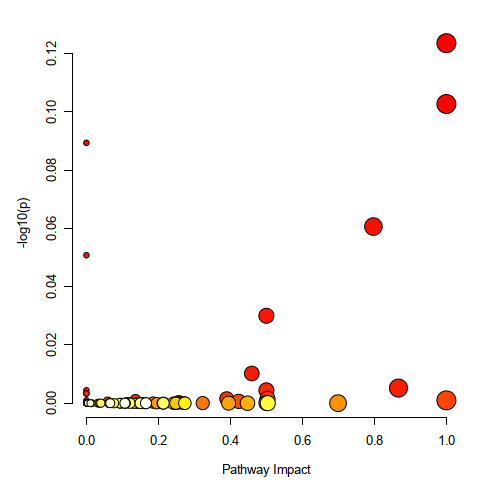
\includegraphics[width=1.0\textwidth]{path_view_0_dpi72.png}
\caption{Summary of Pathway Analysis}
\end{center}
\label{path_view_0_dpi72.png}
\end{figure}
\clearpage


The table below shows the detailed results from the pathway analysis. Since
we are testing many pathways at the same time, the statistical p values from
enrichment analysis are further adjusted for multiple testings. In particular, 
the \textbf{Total} is the total number of compounds in the pathway;
the \textbf{Hits} is the actually matched number from the user uploaded data;
the \textbf{Raw p} is the original p value calculated from the enrichment analysis;
the \textbf{Holm p} is the p value adjusted by Holm-Bonferroni method;
the \textbf{FDR p} is the p value adjusted using False Discovery Rate;
the \textbf{Impact} is the pathway impact value calculated from pathway topology analysis.


